\documentclass[10pt,a4paper,oneside,openany]{book}
\usepackage[T1]{fontenc}
\usepackage[utf8]{inputenc}
\usepackage{lmodern}
\usepackage{microtype}
\usepackage{geometry}
\geometry{top=19mm,bottom=21mm,left=23mm,right=22mm,headheight=23pt}
\usepackage{xcolor,graphicx,amsmath,amssymb,amsthm,mathtools}
\usepackage{booktabs,tabularx,longtable,array,multirow}
\usepackage{enumitem,parskip}
\usepackage[most]{tcolorbox}
\usepackage{tikz}
\usetikzlibrary{arrows.meta,positioning,shapes.geometric,shapes.misc,fit,calc,backgrounds,matrix,decorations.pathreplacing}
\usepackage{pgfplots}
\pgfplotsset{compat=1.18}
\usepackage{titlesec,fancyhdr,lastpage}
\usepackage{float,caption,subcaption}
\usepackage{listings}
\usepackage{hyperref}
\usepackage[capitalise,noabbrev]{cleveref}
\crefname{chapter}{section}{sections}
\Crefname{chapter}{Section}{Sections}
\usepackage{needspace}
\usepackage{multicol}
\definecolor{navy}{HTML}{14243B}
\definecolor{deepblue}{HTML}{20558A}
\definecolor{teal}{HTML}{138F82}
\definecolor{amber}{HTML}{BB772D}
\definecolor{palerblue}{HTML}{EAF2F8}
\definecolor{palerteal}{HTML}{EAF6F4}
\definecolor{paleamber}{HTML}{FBF2E5}
\definecolor{slate}{HTML}{4D6176}
\definecolor{rulegray}{HTML}{D5DEE7}
\definecolor{calloutpink}{HTML}{D96C9F}
\definecolor{calloutpinkbg}{HTML}{FBEAF2}
\definecolor{calloutpurple}{HTML}{7B61A8}
\definecolor{calloutpurplebg}{HTML}{F1ECF8}
\definecolor{calloutred}{HTML}{B84A4A}
\definecolor{calloutredbg}{HTML}{FAEAEA}
\definecolor{calloutgray}{HTML}{6F7780}
\definecolor{calloutgraybg}{HTML}{F1F3F5}
\hypersetup{colorlinks=true,linkcolor=deepblue,urlcolor=teal,citecolor=teal,pdftitle={Machine Learning Foundations},pdfauthor={Prepared for the reader},pdfsubject={Integrated machine learning foundation notes}}
\setlength{\parindent}{0pt}
\setlength{\parskip}{3.5pt plus .7pt minus .4pt}
\setlist[itemize]{topsep=3pt,itemsep=2pt,leftmargin=1.65em}
\setlist[enumerate]{topsep=3pt,itemsep=2pt,leftmargin=1.8em}
\renewcommand{\arraystretch}{1.2}
\captionsetup{font=small,labelfont={bf,color=navy}}
\titleformat{\chapter}[display]{\normalfont}{\Large\bfseries\color{teal}SECTION \thechapter}{8pt}{\Huge\bfseries\color{navy}}[\vspace{3pt}\titlerule]
\titlespacing*{\chapter}{0pt}{-7pt}{13pt}
\titleformat{\section}{\Large\bfseries\color{deepblue}}{\thesection}{.7em}{}
\titleformat{\subsection}{\large\bfseries\color{navy}}{\thesubsection}{.7em}{}
\pagestyle{fancy}
\fancyhf{}
\fancyhead[L]{\small\color{slate}MACHINE LEARNING \textbar\ LESSON NOTES}
\fancyhead[R]{\small\color{slate}\nouppercase{\leftmark}}
\renewcommand{\chaptermark}[1]{\markboth{Section \thechapter: #1}{}}
\fancyfoot[C]{\small\color{slate}\thepage\ / \pageref{LastPage}}
\renewcommand{\headrulewidth}{.3pt}
\renewcommand{\headrule}{\hbox to\headwidth{\color{rulegray}\leaders\hrule height \headrulewidth\hfill}}
\newtcolorbox{calloutexample}[1][]{enhanced,breakable,colback=calloutpinkbg,colframe=calloutpink,boxrule=.6pt,arc=2mm,left=3mm,right=3mm,top=2mm,bottom=2mm,title={\bfseries Example},fonttitle=\color{white},colbacktitle=calloutpink,#1}
\newtcolorbox{calloutpractical}[1][]{enhanced,breakable,colback=calloutpurplebg,colframe=calloutpurple,boxrule=.6pt,arc=2mm,left=3mm,right=3mm,top=2mm,bottom=2mm,title={\bfseries Practical Tip},fonttitle=\color{white},colbacktitle=calloutpurple,#1}
\newtcolorbox{calloutmemorise}[1][]{enhanced,breakable,colback=calloutredbg,colframe=calloutred,boxrule=.6pt,arc=2mm,left=3mm,right=3mm,top=2mm,bottom=2mm,title={\bfseries Memorise},fonttitle=\color{white},colbacktitle=calloutred,#1}
\newtcolorbox{calloutintuition}[1][]{enhanced,breakable,colback=calloutgraybg,colframe=calloutgray,boxrule=.6pt,arc=2mm,left=3mm,right=3mm,top=2mm,bottom=2mm,title={\bfseries Intuition},fonttitle=\color{white},colbacktitle=calloutgray,#1}
\newtcolorbox{calloutbias}[1][]{enhanced,breakable,colback=white,colframe=teal,boxrule=.7pt,arc=2mm,left=3mm,right=3mm,top=2mm,bottom=2mm,title={\bfseries Inductive Bias},fonttitle=\color{white},colbacktitle=teal,#1}
\newcommand{\term}[1]{\textbf{\color{navy}#1}}
\newcommand{\figpdf}[3][.89\textwidth]{\begin{figure}[htbp]\centering\includegraphics[width=#1]{figures/#2.pdf}\caption{#3}\label{fig:#2}\end{figure}}
\newcommand{\code}[1]{\texttt{#1}}
\newcommand{\R}{\mathbb R}
\newcommand{\E}{\mathbb E}
\newcommand{\Var}{\operatorname{Var}}
\newcommand{\Cov}{\operatorname{Cov}}
\newcommand{\KL}{D_{\mathrm{KL}}}
\newcommand{\sgn}{\operatorname{sgn}}
\newcommand{\softmax}{\operatorname{softmax}}
\newcommand{\argmin}{\operatorname*{arg\,min}}
\newcommand{\argmax}{\operatorname*{arg\,max}}
\newcolumntype{Y}{>{\raggedright\arraybackslash}X}
\newcolumntype{L}[1]{>{\raggedright\arraybackslash}p{#1}}
\tikzset{flow/.style={draw=deepblue,fill=palerblue,rounded corners=3pt,align=center,font=\small,inner sep=6pt,minimum height=10mm},
 yesbox/.style={draw=teal,fill=palerteal,rounded corners=3pt,align=center,font=\footnotesize,inner sep=5pt},
 decisionnode/.style={diamond,draw=amber,fill=paleamber,aspect=2.0,align=center,font=\small,inner sep=1pt},
 arr/.style={-{Stealth[length=2.5mm]},thick,draw=slate},
 arrblue/.style={-{Stealth[length=2.5mm]},thick,draw=deepblue}}
\lstdefinestyle{pythonsmall}{language=Python,basicstyle=\small\ttfamily,breaklines=true,keywordstyle=\color{deepblue}\bfseries,stringstyle=\color{teal},commentstyle=\color{slate},showstringspaces=false,backgroundcolor=\color{palerblue},frame=single,rulecolor=\color{rulegray},columns=fullflexible,keepspaces=true,aboveskip=6pt,belowskip=6pt}
\lstset{style=pythonsmall}



% Token

% Token formatting -- compatible with Overleaf's default pdfLaTeX
\usepackage[T1]{fontenc}
\usepackage{lmodern}
\usepackage{amsmath}
% Literal token spellings, including underscores, pipes and brackets
\DeclareRobustCommand{\tok}[1]{%
    \begingroup
    \ttfamily
    \detokenize{#1}%
    \endgroup
}
% Visible ASCII substitutes for Unicode whitespace markers
% GPT-2/RoBERTa: Ġ (U+0120)
\newcommand{\gspace}{\texttt{[SP]}}
% SentencePiece: ▁ (U+2581)
\newcommand{\spmspace}{\texttt{[SPM]}}



\begin{document}

\begin{titlepage}
\thispagestyle{empty}
\begingroup
\definecolor{atlascream}{HTML}{F9E3AC}
\begin{tikzpicture}[remember picture,overlay]
  % Full bleed A4: fills the page exactly. The original image is 2:3,
  % so there is a small horizontal stretch to A4 (210:297).
  \node[anchor=center,inner sep=0] at (current page.center) {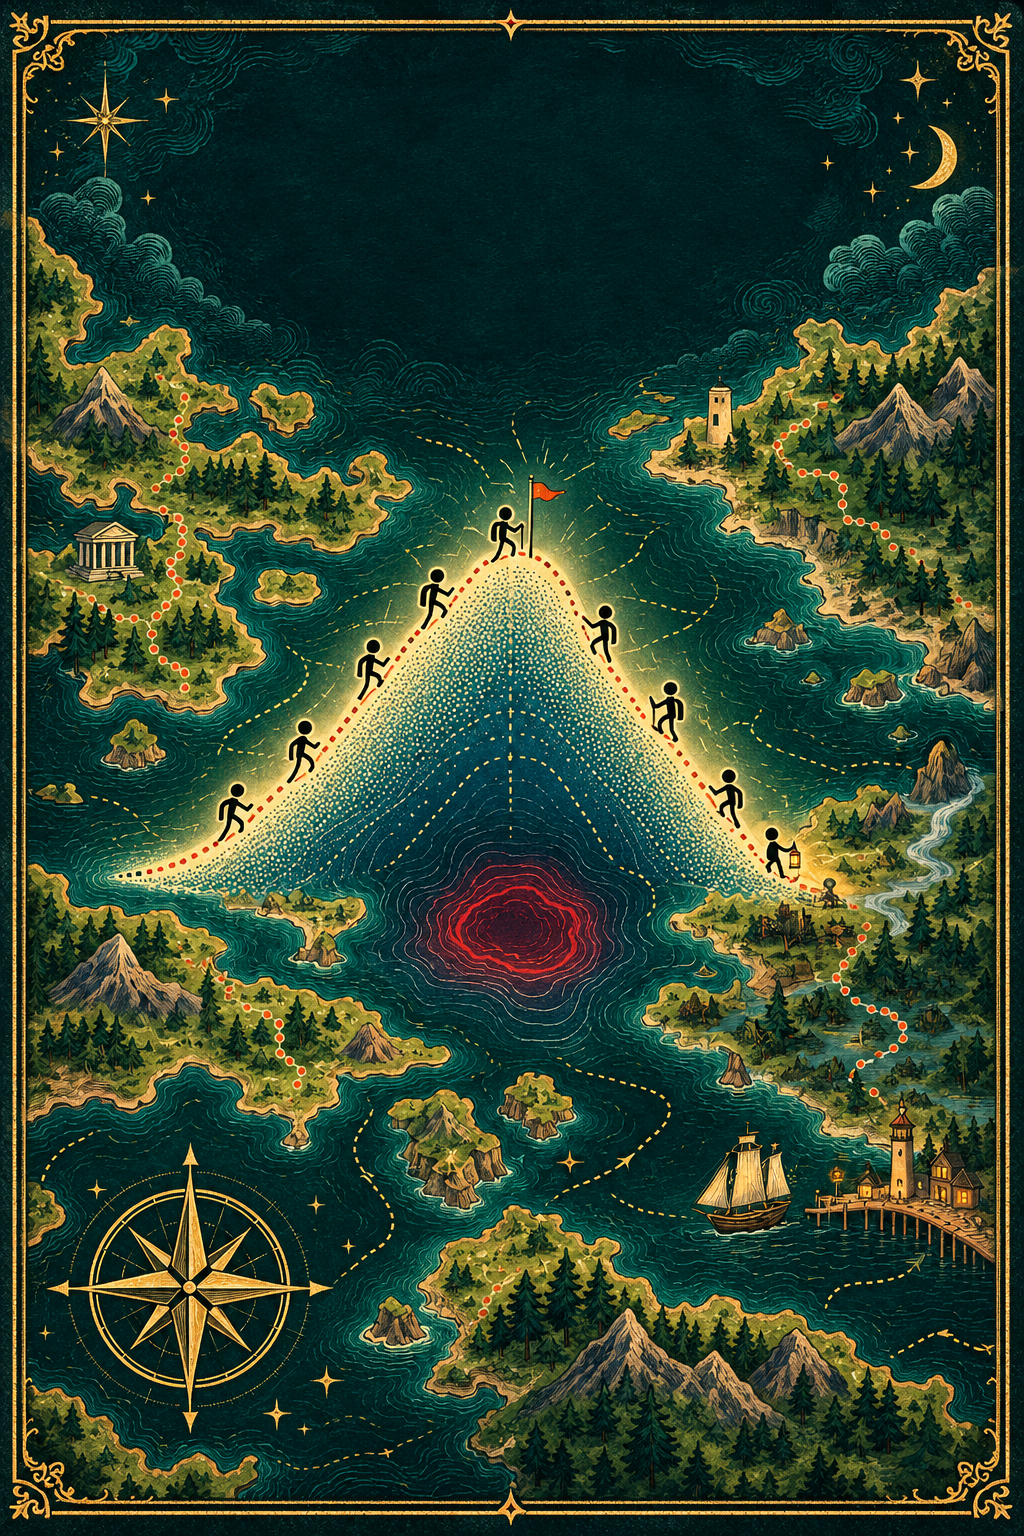
\includegraphics[width=\paperwidth,height=\paperheight]{figures/atlas_background.png}};

  % Text overlays; distances are from the top of the A4 page.
  \node[anchor=north,align=center,text=atlascream,inner sep=0pt]
    at ([yshift=-30mm]current page.north)
    {{\fontfamily{ppl}\selectfont\bfseries\fontsize{43}{49}\selectfont Henry's ML Atlas}};

  \node[anchor=north,align=center,text=atlascream,inner sep=0pt]
    at ([yshift=-50mm]current page.north)
    {{\fontfamily{ppl}\selectfont\fontsize{14.2}{18}\selectfont Machine Learning Revision Notes}};

  \node[anchor=north,align=center,text=atlascream,inner sep=0pt]
    at ([yshift=-63mm]current page.north)
    {{\fontfamily{ppl}\selectfont\fontsize{13}{16}\selectfont September 2026}};
\end{tikzpicture}
\null
\endgroup
\end{titlepage}

\frontmatter
\hypersetup{pageanchor=true}
\tableofcontents
% Additional callout environments used by the front matter and available to later sections.
% These live here so the main document and lesson files remain untouched.
\newtcolorbox{calloutspecialcase}[1][]{enhanced,breakable,colback=paleamber,colframe=amber,boxrule=.6pt,arc=2mm,left=3mm,right=3mm,top=2mm,bottom=2mm,title={\bfseries Special Case},fonttitle=\color{white},colbacktitle=amber,#1}
\newtcolorbox{calloutmemoryhook}[1][]{enhanced,breakable,colback=palerblue,colframe=deepblue,boxrule=.6pt,arc=2mm,left=3mm,right=3mm,top=2mm,bottom=2mm,title={\bfseries Memory Hook},fonttitle=\color{white},colbacktitle=deepblue,#1}
\newtcolorbox{calloutdegreeofexperiment}[1][]{enhanced,breakable,colback=white,colframe=navy,boxrule=.7pt,arc=2mm,left=3mm,right=3mm,top=2mm,bottom=2mm,title={\bfseries Degree of Experiment},fonttitle=\color{white},colbacktitle=navy,#1}

\chapter*{Initial Commentary}
\addcontentsline{toc}{chapter}{Initial Commentary}
\markboth{Initial Commentary}{Initial Commentary}

\subsection*{Goals}
\addcontentsline{toc}{section}{Goals}
This book is not aimed at a student, graduate, or academic learning machine learning from scratch.
It is a revision tool intended to give a high-level understanding of the wide research area we call ML.
Being targeted at senior or expert-level practitioners looking for a refresher, update, or review, this book aims to:

\begin{itemize}
    \item represent the topics mental model quickly
    \item connect topics to the assumptions, consequences, and neighbouring ideas
    \item expose the design choices and research degrees of freedom around a method
\end{itemize}

\subsection*{Philosophy}
\addcontentsline{toc}{section}{Philosophy}
This book follows Henry's learning policies:

\begin{itemize}
    \item \textbf{Allow the reader their own language.}
    Learning is done by understanding, and we all understand in different ways.
    Leaving naming to the reader gives the reader maximum space to use their own definitions.
    It also means that we can rely on the maths talking for us, and we do not need long ``where $X$ is $Y$ and $A$ is $B$'' text surrounding maths.
    For this reason, favour descriptive mathematics, or even ``plain English equations''.
    Some examples:
    \begin{itemize}
        \item Instead of using the Jacobian, $J$, in an expression, use its base definition $\left(\frac{\partial y}{\partial x}\right)$ where that is clearer. If the fact that it is a Jacobian matters, an underbrace can name the term without introducing another symbol.
        \item Instead of assigning counts to arbitrary letters, use descriptive subscripts such as $N_{\text{experts}}$ or $N_{\text{trees}}$.
        \item The term $\lambda_{\text{e-val(A)}}$ is clearly representing the eigenvalue of matrix A without wasting text space.
    \end{itemize}

    \item \textbf{Short and sweet.}
    Some textbooks spell out everything for the reader, making reading passive.
    Jumping a few logical steps and naming a conclusion rather than reproducing a full derivation makes reading active: the reader fills in the small gaps in their own terms.

    \item \textbf{Minimal mathematics, maximum intuition.}
    The reader should not need to wade through definitions and mathematical fuckery to understand a topic.
    After one read they should be able to discuss and reason around a topic.

    \item \textbf{Minimal jargon.}
    Some technical vocabulary is necessary, but terminology should earn its place.
    Prefer descriptive plain-English wording when a specialist label does not add useful precision.
    Henry believes that humans naturally obscure their discoveries to nurse their own ego, and impress others - avoid this. 
    
    \item \textbf{Memory Hook.}
    A Memory Hook is a short sentence that encodes information and acts as a retrieval cue for a much larger mental model.
    People struggle to memorise large amounts of text and maths, but often remember a compact story or rule quickly.
    Therefore, explain the story as concisely as possible and summarise it with a Memory Hook.
    Some synonyms I have heard them described as: micro-heuristics, concept capsules, retrieval rules, compressed principles, rules of thumb, Compressed Heuristics, Knowledge in One Breath, High-Leverage Facts, or simply Memory Hooks. 
    They may be further split into categories:
    \begin{itemize}
        \item \textbf{Mechanisms}. e.g: \textit{Vanishing gradients make early layers slow learners}, e.g: \textit{More parameters reduce bias; regularisation restrains variance}.
        \item \textbf{Actions}. e.g: \textit{With ReLU activations, start with He/Kaiming initialisation to handle the negatives}.
        \item \textbf{Special Cases}. e.g: \textit{L1 Regularisation is basically feature selection}.
        \item \textbf{Differentiator}. e.g: \textit{AdamW seperates weight decay and scaling; adding an L2 penalty inside Adam does not produce the same update}.
    \end{itemize}
    Once memorised, one should be able to rebuild a mental model of each sub-topic from a single sentence and reason outward from that sentence.
    \item \textbf{Analogies.} Analogies are vital for bridging gaps, unifying across diffuse fields and intuition.
\end{itemize}



\subsection*{Assumed Understanding}
\addcontentsline{toc}{section}{Assumed Understanding}

Because this is aimed at revision rather than first-time teaching, we do not need to dive into easy material.
We assume some knowledge of linear algebra (for example, what orthogonal means), basic maths (differentiation, the chain rule, probability), computer science (for example, what a bit is), physics-style reasoning (for example, entropy), and basic world knowledge (for example, what an image is).
If a prerequisite is only needed to understand one consequence, remind the reader of the minimum required fact rather than reteaching the whole prerequisite topic.

\subsection*{How to Read This}
\addcontentsline{toc}{section}{How to Read This}

This textbook is not a ``teach me ML'' book with full derivations and exhaustive depth.
It is a high-level overview of key points, with a focus on links, consequences, design choices, and practical usage.
A few examples:

\begin{enumerate}
    \item We teach how Adam interacts with L2 regularisation and why AdamW changes the update; we do not derive convergence boundaries.
    \item We describe the evolution of tree architectures as an accumulation of methods and ideas toward modern systems; we do not provide an end-to-end derivation of every incremental algorithm.
    \item We explain what a design choice changes, which assumptions make it sensible, and what failure mode it addresses; we do not catalogue every historical variant simply because it exists.
\end{enumerate}

A useful reading pattern is: \textbf{mechanism $\rightarrow$ consequence $\rightarrow$ trade-off $\rightarrow$ practical choice}.
Equations, figures, timelines, and callouts exist to compress that chain, not to interrupt it.

\subsection*{Types of Callout}
\addcontentsline{toc}{section}{Types of Callout}
Callouts are used strictly for these rules, but are often memory hooks. 

\begin{calloutexample}
A concrete worked or real-world instance of the idea just described.
For example: \textit{if two classifiers have the same accuracy but one misses nearly all rare positive cases, class imbalance has made accuracy hide the behaviour we actually care about.}
\end{calloutexample}

\begin{calloutpractical}
A directly useful action, implementation choice, or debugging rule.
For example: \textit{With ReLU activations, start with He/Kaiming initialisation.}
\end{calloutpractical}

\begin{calloutmemorise}
A fact or equation that is worth recalling accurately rather than reconstructing each time.
For example:
\[
\operatorname{softmax}(z_i)=\frac{e^{z_i}}{\sum_j e^{z_j}}.
\]
\end{calloutmemorise}

\begin{calloutintuition}
A compact way to think about a mechanism without pretending the analogy is the full definition.

\textit{L1 regularisation is basically feature selection on weight abs-size.}
\end{calloutintuition}

\begin{calloutbias}
State the assumption a method builds in, what that assumption buys us, and when it can become a restriction.
Use the form: \textit{if \textless assumption/data/method\textgreater, then \textless consequence\textgreater}.

For example: \textit{if nearby pixels are more related than distant pixels, convolution's locality bias is useful; if feature order is arbitrary, that same bias may be inappropriate.}
\end{calloutbias}

\begin{calloutspecialcase}
A useful reduction where a broader idea becomes a familiar one under a particular setting.
For example: \textit{the F1 score is the special case of the F$\beta$ score with $\beta=1$}.
\end{calloutspecialcase}

\begin{calloutmemoryhook}
One sentence that should let the reader reconstruct a larger mental model.
It may encode a mechanism, action, special case, or differentiator.
For example: \textit{Vanishing gradients make early layers slow learners.}
\end{calloutmemoryhook}

\begin{calloutdegreeofexperiment}
A dimension along which researchers or experimenters can change a system while keeping the broader method recognisable.
For example, for normalisation one can vary \textit{which axes define the statistics, where normalisation is inserted, whether the statistics depend on the batch, and whether learned scale/shift parameters are used}.
\end{calloutdegreeofexperiment}

\subsection*{Formatting and AI Guide}
\addcontentsline{toc}{section}{Formatting Guide}

\subsubsection*{AI Editing Rules}
\addcontentsline{toc}{section}{AI Editing Rules}

AI edits should behave like careful maintenance of one coherent textbook, not like a fresh author rewriting the surrounding material.

\begin{enumerate}
    \item \textbf{Respect the Initial Commentary.} Conduct work with Goals, philosophy and formatting in context. 

    \item \textbf{Respect edit scope.} Change only the material requested. 
    Do not silently rewrite other sections.

    \item \textbf{Integrate; do not append.} New work belongs at the point in the existing text where the concept is most relevant. 
    Do not create a trailing ``questions'', ``additional notes'', or ``follow-ups'' section unless explicitly requested.
    Add to sections, tables, reference it, etc.

    \item \textbf{Use the callout taxonomy literally.} Example = concrete instance; Practical Tip = action; Memorise = exact recall; Intuition = mental model; Inductive Bias = assumption $\rightarrow$ consequence; Special Case = useful reduction; Memory Hook = compressed retrieval cue; Degree of Experiment = research/design axis. Do not create callout categories.

    \item \textbf{Cross-reference before duplicating.} If the prerequisite idea is already taught elsewhere, link to it and provide only the minimum reminder needed locally.

    \item \textbf{Use visuals for structure.} All visuals need visual reviewing, never 'tkviz and forget'. 

    \item \textbf{Preserve document mechanics.} Keep labels, references, equations, figures, terminology, and LaTeX conventions consistent with the existing book. 
    After edits, compile and visually verify the affected pages rather than assuming valid source means valid layout.
\end{enumerate}


\subsubsection*{Tone}
\addcontentsline{toc}{section}{Tone}

This is informal for a textbook, but it should remain clear and technically precise.
For example: ``\code{L1 regularisation is basically feature selection on abs(weights)}''.
Here, \code{abs(weights)} is deliberate shorthand for the more long-winded ``absolute size of the weights''.
Shorthand is welcome when it compresses an idea without changing its meaning.


\subsubsection*{Prose and hierarchy}

\begin{itemize}
    \item New latex line per sentence (not a new compiled/pdf line!)
    \item Prefer short paragraphs. 
    A paragraph should normally carry one conceptual step: mechanism, consequence, contrast, or caveat.
    \item Use \textbf{bold} for the local concept that the sentence is about, \textit{italics} for compact rules or deliberately memorable phrasing, and \code{monospace} for code-like shorthand such as \code{abs(weights)}.
    \item Introduce jargon only when the term will be useful later. If the plain-English phrase is clearer, use it first and put the formal name next to it in bold.

\end{itemize}

\subsubsection*{Mathematics}

\begin{itemize}
    \item Use equations when the mathematical relationship itself is the memory hook, when notation is more compact than prose, or when a downstream consequence depends on the form of the equation.
    \item Prefer descriptive notation and subscripts over arbitrary letters. Avoid introducing a symbol merely to save one line of typing.
    \item Do not include a derivation by default. Show the minimal step needed to expose the mechanism or consequence.
    \item When a particular equation is genuinely recall-worthy, put it in a \textbf{Memorise} callout. Most equations should remain ordinary body content.
    \item Explain non-obvious terms next to the equation, but do not spell out standard notation the assumed reader already knows.
    \item Generally, condense an idea down to one equation through labelling and substitution. 
    For example, the Adam equation is often expressed as 
    \[
        \theta_{t+1}=\theta_t-\eta\frac{\hat m_t}{\sqrt{\hat v_t}+\epsilon}
    \]
    with some definitions, but we prefer a 'whole story' equation:
    \[
        \theta_{t+1}
        =
        \theta_t-\eta
        \frac{
        \overbrace{\beta_1m_{t-1}+(1-\beta_1)g_t}
        ^{\substack{= m_t , \text{momentum}}}
        }{
        \sqrt{
        \underbrace{\beta_2v_{t-1}+(1-\beta_2)g_t^{2}}
        _{\substack{= v_t , \text{scale}}}
        }+\epsilon
        }
    \]
    \item Some non-standard notation, which we standardise here:
    \begin{itemize}
        \item Model Weights $w$ should be represented as parameter weights: $\theta_{\text{weights}}$.
        \item Any count is $N$ with an english subscript.
        \item Indexing a matrix if with subscripts like $A_{ij}$ and selecting a matrix subset is pythonic like $A_{[:i]}$ for the first i columns of $A$.
    \end{itemize}
    
    
\end{itemize}

\subsubsection*{Research evolution}

When methods evolved through a recognisable sequence show the evolution as an accumulation of problems/fixes rather than as isolated definitions.
A compact table-timeline is preferred when it makes the sequence clear.
The goal is not historical completeness. 
Include the steps that change the reader's mental model of the modern method.

\begin{center}
\small
\begin{tabularx}{0.96\textwidth}{@{}L{0.17\textwidth}L{0.22\textwidth}Y Y@{}}
\toprule
\textbf{Step} & \textbf{What changed} & \textbf{Why it was added} & \textbf{Consequence / new trade-off} \\
\midrule
Baseline & Starting mechanism & What it cannot do well & The limitation that motivates the next step \\
Next method & One important addition & Which limitation it targets & What improves, plus what becomes more complex or biased \\
Modern variant & Further separation or control & Which earlier coupling/failure it fixes & Current practical behaviour and remaining choices \\
\bottomrule
\end{tabularx}
\end{center}

\subsubsection*{Callout discipline}

A useful test is whether the boxed text can be removed without breaking the main explanation: the body should still teach the topic, while the callout should provide a separable retrieval cue, action, example, or qualification.
Avoid stacking several callouts in a row in ordinary chapters.

\subsubsection*{Formatting Example}

The following miniature section demonstrates the intended rhythm: short mechanism, minimal maths, then a small number of purpose-specific callouts.

\paragraph{L1 regularisation.}
Add a penalty proportional to the absolute size of the parameters:
\[
\mathcal{L}_{\text{total}}
=
\mathcal{L}_{\text{data}}
+
\lambda\sum_i |w_i|.
\]
The penalty has a constant-magnitude pull toward zero away from zero, so weakly useful parameters are more likely to be driven exactly to zero than under an L2 penalty. The practical consequence is sparse parameter vectors and, in models where weights map directly to input features, an effect similar to feature selection.

\begin{calloutintuition}
\textit{L1 is basically feature selection on weight abs-size.}
\end{calloutintuition}

\begin{calloutexample}
In a linear model with thousands of candidate input features, increasing $\lambda$ can drive many feature weights to exactly zero, leaving a smaller active subset.
\end{calloutexample}

\begin{calloutdegreeofexperiment}
The research/design knobs include the penalty strength $\lambda$, which parameter groups are penalised, whether sparsity is applied to individual weights or structured groups, and whether sparsity is imposed during training or by a later pruning step.
\end{calloutdegreeofexperiment}

This is the intended level of depth: enough mathematics to expose the mechanism, enough consequence to make the choice useful, and no derivation that does not change the mental model.
\mainmatter
\chapter{Foundations: Mathematics}
\label{chap:foundations}

\section{Linear maps, directions and information}
\label{sec:foundations-linear-maps-directions-and-information}
\label{sec:la-vector-geometry-and-linear-independence}
\label{sec:la-matrices-as-linear-transformations}

For ML, the useful geometric question is usually not ``what is a vector?'' but ``which directions contain distinct information, and what does a transformation preserve or destroy?''
For nonzero vectors, the dot product separates magnitude from directional alignment:
\[
\underbrace{x^\top y}_{\text{magnitude + alignment}}
=
\|x\|\,\|y\|\underbrace{\cos\phi}_{\text{directional alignment}},
\qquad
x\perp y\iff x^\top y=0.
\]
Cosine similarity removes magnitude; the raw dot product does not.
This distinction matters in embeddings and similarity search when vector norm may or may not carry task information.
\label{subsec:la-dot-product}
\label{subsec:la-orthogonality}


\subsection{Independence, span, rank and null space}
\label{subsec:la-linear-independence}
\label{subsec:la-span-and-rank}
\label{subsec:la-image-space-and-null-space}
\label{subsec:la-singular-matrices}

\textbf{Linear independence} means a direction cannot be reconstructed from the others; the \textbf{span} is everything their combinations can represent; \textbf{rank} counts independent surviving directions.
For a linear map $y=Ax$, rank--nullity gives the information-capacity picture directly:
\begin{equation}
    \underbrace{N_{\text{input dimensions}}}_{\text{available directions}}
    =
    \underbrace{\operatorname{rank}(A)}_{\text{directions that survive}}
    +
    \underbrace{\dim\ker(A)}_{\text{directions destroyed}}
.
\end{equation}
The image/column space is what the map can output; the null space contains input perturbations that become invisible.
Redundant features and low-rank parameterisations are both statements about how many independent directions are actually needed.
This is the prerequisite for PCA in \cref{sec:representation-pca-an-eigenvector-view} and LoRA in \cref{sec:adaptation-lora-a-parameter-efficient-adaptation-mechanism}.

\begin{calloutmemoryhook}
Rank counts independent directions (columns of matrix); the null space counts directions the map deletes.
\end{calloutmemoryhook}

An inverse exists only when a square linear map loses no direction and covers its output space.
In numerical ML code, solve a linear system or use a factorisation rather than explicitly forming $A^{-1}$ unless the inverse itself is required.
\label{subsec:la-inverse-of-a-matrix}
\label{subsec:la-determinant}

\section{Eigenstructure and low-rank structure}
\label{sec:foundations-eigenstructure-and-low-rank-structure}
\label{sec:la-eigenstructure-and-matrix-properties}

\subsection{Eigenvectors, eigenvalues and PSD structure}
\label{subsec:la-eigenvectors-and-eigenvalues}
\label{subsec:la-positive-semi-definite-psd-matrices}

An eigenvector is a direction a linear map does not rotate away from itself:
\[
A\underbrace{v}_{\text{preserved direction}}
=
\underbrace{\lambda_{\text{along }v}}_{\text{scale on that direction}}v.
\]
The same mental model appears in covariance/PCA, recurrent dynamics and curvature: eigenvectors identify special directions; eigenvalues say how strongly the operator acts along them.
PCA uses covariance eigenstructure explicitly in \cref{sec:representation-pca-an-eigenvector-view}; the optimisation consequence reappears with Hessian curvature in \cref{sec:optimisation-newton-s-method-and-other-second-order-methods}.

A symmetric matrix is positive semidefinite (PSD) when
\[
\underbrace{x^\top A x}_{\text{quadratic response along }x}\ge 0\qquad\text{for every }x.
\]
For symmetric $A$, this is equivalent to nonnegative eigenvalues.
Covariance matrices are PSD.
\begin{calloutmemoryhook}
A PSD Hessian means convex space.
\end{calloutmemoryhook}

\subsection{SVD as the rectangular low-rank view}
\label{subsec:foundations-svd}

For a rectangular matrix, singular value decomposition exposes the same directional story without requiring a square matrix:
\[
A
=
\underbrace{U}_{\text{output directions}}
\underbrace{\Sigma}_{\text{direction-wise scales}}
\underbrace{V^\top}_{\text{input directions}}.
\]
Large singular values identify directions the map transmits strongly; truncating small ones gives a low-rank approximation.
That is the common structural idea behind compression, PCA implementations and parameter-efficient low-rank updates such as LoRA (\cref{sec:adaptation-lora-a-parameter-efficient-adaptation-mechanism}).

\section{Probability, uncertainty and estimation}
\label{sec:foundations-pmfs-and-pdfs}

For a discrete random variable, a PMF assigns probability mass and sums to one; for a continuous variable, a PDF integrates to one and probabilities are areas under the density.
Conditional and joint distributions connect through $p(x,y)=p(y\mid x)p(x)$; marginalisation removes variables by summing or integrating them out.

\subsection{Expectation, variance and covariance}
\label{sec:foundations-expectation-variance-and-covariance}

Expectation is the distribution-weighted average.
Variance and covariance capture spread and linear co-variation:
\begin{align}
\Var(X)
&=\E\!\left[(X-\E[X])^2\right],\\
\Cov(X,Y)
&=\E\!\left[(X-\E[X])(Y-\E[Y])\right],\\
\rho_{XY}
&=\frac{\Cov(X,Y)}{\sqrt{\Var(X)\Var(Y)}}.
\end{align}
Zero covariance is weaker than independence; independence implies zero covariance when the relevant moments exist.
For vector-valued data, the covariance matrix $\Sigma=\E[(x-\E[x])(x-\E[x])^\top]$ packages pairwise linear co-variation and feeds directly into PCA/whitening in \cref{sec:representation-pca-an-eigenvector-view,sec:representation-whitening-pca-and-zca}.


\subsection{Bayes, likelihood and priors}
\label{sec:foundations-bayes-theorem}

\begin{calloutmemorise}
\[
\boxed{P(A\mid B)=\frac{P(B\mid A)P(A)}{P(B)}}.
\]
\end{calloutmemorise}
Bayes' rule says a posterior combines prior belief with how compatible the observation is under each hypothesis.
For rare events, the prior/base rate can dominate the interpretation of a positive test; this is the probability-side version of precision in \cref{sec:evaluation-precision-recall-and-f1}.

\begin{calloutexample}
If prevalence is $1\%$, sensitivity is $95\%$, and the false-positive rate is $5\%$, then $P(\text{fault}\mid +)\approx16\%$: a sensitive detector can still produce mostly false alarms when the event is rare.
\end{calloutexample}

\label{sec:foundations-maximum-likelihood-and-maximum-a-posteriori-estimation}
For $N_{\text{examples}}$ conditionally independent observations, maximum likelihood chooses parameters that maximise summed log-likelihood:
\[
\hat\theta_{\mathrm{MLE}}
=
\argmax_{\theta}\sum_{i=1}^{N_{\text{examples}}}\log p(x_i\mid\theta).
\]
MAP adds a prior preference directly to the same objective:
\[
\hat\theta_{\mathrm{MAP}}
=
\argmax_{\theta}
\left[
\underbrace{\log p(D\mid\theta)}_{\text{fit to observations}}
+
\underbrace{\log p(\theta)}_{\text{parameter preference}}
\right].
\]
Gaussian-like priors produce L2-style penalties; Laplace-like priors produce L1-style penalties, linking Bayesian preference to regularisation in \cref{sec:stability-regularisation-l1-and-l2} and inductive bias in \cref{sec:nfl-bayesian-priors-a-direct-form-of-inductive-bias}.

\subsection{Entropy and distribution mismatch}
\label{sec:foundations-entropy}

\begin{calloutmemorise}
\[
\boxed{H(X)=-\sum_x p(x)\log p(x)}.
\]
\end{calloutmemorise}
Entropy measures uncertainty in one distribution.
Cross-entropy measures coding/surprise when observations follow $p$ but predictions use $q$; KL is the extra cost relative to using $p$ itself:
\label{sec:foundations-cross-entropy-kl-divergence-and-jensen-shannon-divergence}
\[
\underbrace{H(p,q)}_{\text{cross-entropy}}
=
\underbrace{H(p)}_{\text{irreducible uncertainty}}
+
\underbrace{D_{\mathrm{KL}}(p\|q)}_{\text{mismatch penalty}}.
\]
KL is asymmetric and can be infinite when $q$ assigns zero probability where $p$ does not.
Jensen--Shannon divergence symmetrises this comparison through the mixture $(p+q)/2$ and is bounded.
Cross-entropy becomes a classification objective in \cref{sec:objectives-classification-losses-and-logits}; entropy reduction also drives common tree-split criteria in \cref{subsec:trees-learning-a-split}.

\section{Local Derivatives and Curvature}
\label{sec:la-multivariable-calculus-and-optimisation}

\subsection{Jacobian: local input-to-output sensitivity}
\label{subsec:la-jacobian}

For a vector-valued map $f:x\mapsto y$, the local first-order response is
\[
\Delta y
\approx
\underbrace{\frac{\partial y}{\partial x}}_{\text{Jacobian: local sensitivity map}}\Delta x.
\]
The Jacobian tells which input directions are amplified, suppressed or locally invisible; its products are the algebra underneath backpropagation and recurrent gradient propagation.
See \cref{sec:optimisation-backpropagation-how-gradients-are-calculated,sec:stability-weight-initialisation-start-in-a-trainable-region} for those consequences rather than reteaching them here.

\begin{calloutmemoryhook}
The Jacobian maps a small input perturbation to its first-order output perturbation.
\end{calloutmemoryhook}

\subsection{Hessian: local curvature of a scalar objective}
\label{subsec:la-hessian}

For a scalar loss, the second derivative matrix controls the local quadratic correction:
\[
\mathcal L(\theta+\Delta)
\approx
\mathcal L(\theta)
+
\nabla_\theta\mathcal L(\theta)^\top\Delta
+
\frac12\Delta^\top
\underbrace{\nabla_\theta^2\mathcal L(\theta)}_{\text{Hessian: local curvature}}\Delta.
\]
Large positive Hessian eigenvalues mean sharp positive curvature; small magnitudes mean flat directions; negative eigenvalues identify locally downhill curvature directions around a saddle/non-minimum.
Newton and curvature-aware methods use this structure in \cref{sec:optimisation-newton-s-method-and-other-second-order-methods}.

\subsection{Convexity}
\label{sec:foundations-convexity-and-why-it-matters-for-optimisation}

A convex objective has no suboptimal local minima: averaging two parameter points cannot raise the function above the corresponding average of their objective values.
For twice-differentiable objectives on a convex domain, a PSD Hessian everywhere is the useful local test.
Deep-network losses are generally nonconvex, so convex guarantees do not transfer automatically.

\section{Confidence intervals and standard error}
\label{sec:foundations-confidence-intervals}

For $N_{\text{independent observations}}$ with sample standard deviation $s$, the mean estimator has standard error
\[
\operatorname{SE}(\hat\mu)=\frac{s}{\sqrt{N_{\text{independent observations}}}}.
\]
A confidence interval is a sampling-procedure statement, not a posterior probability that the fixed parameter lies in the realised interval.
Use a Student-$t$ critical value for normally distributed observations with unknown variance and small samples; use resampling or a model matched to the dependence structure when independence is not credible.
Evaluation-specific consequences are revisited in \cref{sec:evaluation-cross-validation-and-fold-choice,sec:evaluation-model-selection-and-data-leakage}.


\chapter{Foundations: Data Systems}
\label{chap:data-systems}

\section{The central idea}
\label{sec:data-systems-central-idea}

A data system is mostly a set of decisions about where data lives, how it is represented, and how you expect to access it.

An \textbf{Access Pattern} can be thought of as a systems inductive bias.
\begin{itemize}
    \item CNN: locality
    \item Transformer: interactions should be learnable through attention
    \item Redis assumes that the key$\rightarrow$value is the limiting operation
    \item columnar format assumes we read a few columns across many rows
    \item vector database assumes that nearby embeddings represent semantically similar items
\end{itemize}

Understanding the \textbf{bias} usually tells you when to use the system.

\section{Overview}
\label{sec:data-systems-overview}

\begin{figure}[htbp]
\centering
\resizebox{0.98\linewidth}{!}{%
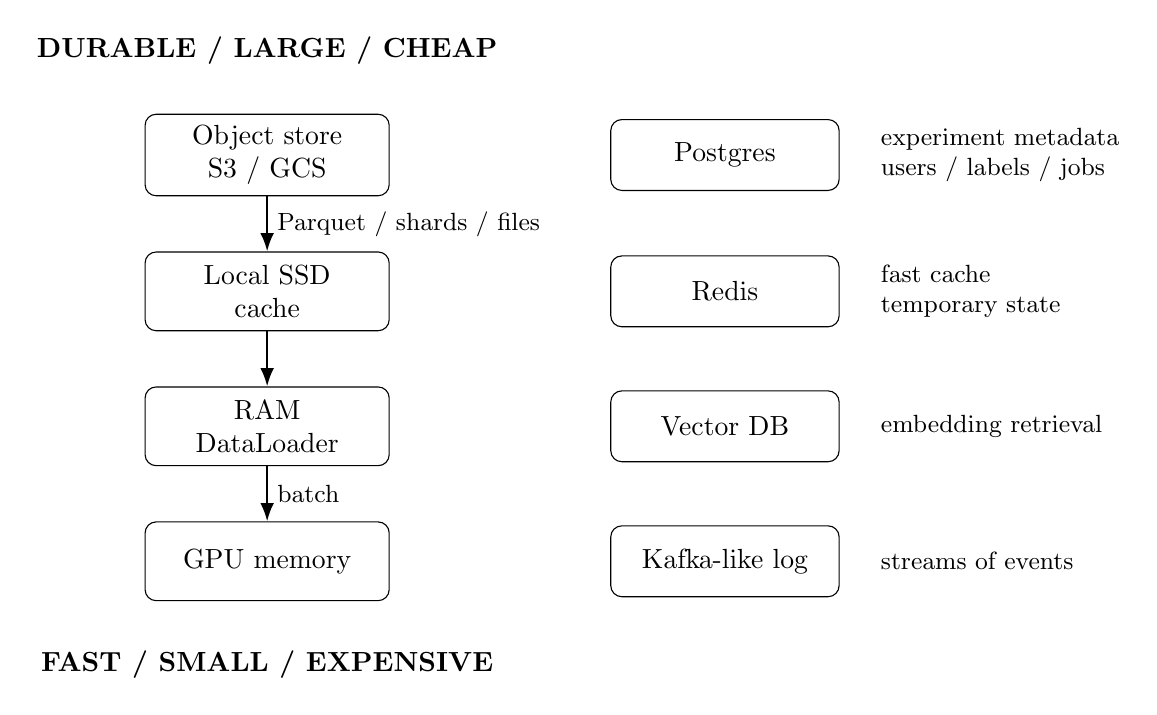
\begin{tikzpicture}[
  >=Latex,
  node distance=7mm and 13mm,
  box/.style={draw, rounded corners, align=center, minimum width=31mm, minimum height=10mm, inner sep=4pt},
  smallbox/.style={draw, rounded corners, align=center, minimum width=29mm, minimum height=9mm, inner sep=3pt},
  arrow/.style={->, thick},
  note/.style={align=left, font=\small}
]
\node[align=center,box] (object) {Object store\\S3 / GCS};
\node[align=center,box, below=of object] (ssd) {Local SSD\\cache};
\node[align=center,box, below=of ssd] (ram) {RAM\\DataLoader};
\node[box, below=of ram] (gpu) {GPU memory};

\draw[arrow] (object) -- node[right, note]{Parquet / shards / files} (ssd);
\draw[arrow] (ssd) -- (ram);
\draw[arrow] (ram) -- node[right, note]{batch} (gpu);

\node[smallbox, right=28mm of object] (pg) {Postgres};
\node[align=center,note, right=4mm of pg] {experiment metadata\\users / labels / jobs};

\node[smallbox, right=28mm of ssd] (redis) {Redis};
\node[align=center,note, right=4mm of redis] {fast cache\\temporary state};

\node[smallbox, right=28mm of ram] (vector) {Vector DB};
\node[note, right=4mm of vector] {embedding retrieval};

\node[smallbox, right=28mm of gpu] (kafka) {Kafka-like log};
\node[note, right=4mm of kafka] {streams of events};

\node[align=center, font=\bfseries, above=5mm of object] {DURABLE / LARGE / CHEAP};
\node[align=center, font=\bfseries, below=5mm of gpu] {FAST / SMALL / EXPENSIVE};
\end{tikzpicture}%
}
\caption{A useful first mental model for an ML data system. Data moves from durable, large storage toward progressively faster and smaller memory as computation approaches the GPU. Other stores serve different access patterns rather than forming one single hierarchy.}
\label{fig:data-systems-master-picture}
\end{figure}


\begin{table}[htbp]
\centering
\caption{The recurring questions to ask about every storage or data-system component. 
You should be able to look at each arrow in Figure \ref{fig:data-systems-master-picture} and ask what the requirements are, based on Table \ref{tab:data-systems-six-questions}.
}
\label{tab:data-systems-six-questions}
\begin{tabularx}{\linewidth}{@{}lX@{}}
\toprule
\textbf{Property} & \textbf{Question} \\
\midrule
Capacity & How much data can this layer hold economically? \\
Latency & How long does one access take before useful data begins arriving? \\
Bandwidth & How much data can move per second once transfer is underway? \\
Cost & What do storage, memory, compute, and network traffic cost? \\
Durability & What happens to the data after crashes or machine loss? \\
Access pattern & Exact lookup, range query, scan, stream, similarity search, or sequential read? \\
\bottomrule
\end{tabularx}
\end{table}

\clearpage
\section{Data structures}
\label{sec:data-structures}

\subsection{Arrays and Tensors}
\label{subsec:arrays-native-language}
An array is conceptually a structured set of filled memory dimensions. 
The important property is that elements are laid out predictably in memory.
\begin{verbatim}
memory: [3.2][1.7][8.1][0.4][2.9]
\end{verbatim}

A tensor is essentially:
\begin{verbatim}
array:
    shape
    dtype
    strides
    device
\end{verbatim}

For example,$\overbrace{X}^{\text{tensor}} \in
\mathbb{R}^{\overbrace{32}^{\text{images}}
\times \overbrace{3}^{\text{channels}}
\times \overbrace{224}^{\text{height}}
\times \overbrace{224}^{\text{width}}}$
might mean 32 images, 3 channels, 224 pixels, 224 pixels.

\paragraph{Efficiency}
Suppose the CPU asks for \verb|X[100]|.
The address can essentially be calculated directly without a costly search operation.
This gives approximately constant-time random access.
\[
\underbrace{a_{100}}_{\text{address of element 100}}
=
\underbrace{a_0}_{\text{base address}}
+
\underbrace{100}_{\text{index}}
\times
\underbrace{s}_{\text{bytes per element}}.
\]


\paragraph{Memory locality}

Processors rarely fetch exactly one number.
They fetch blocks of nearby memory into caches.
So reading
\begin{verbatim}
X[0],X[1],X[2],X[3]
\end{verbatim}
is generally much friendlier than
\begin{verbatim}
X[2],X[92817],X[71],X[831]
\end{verbatim}
This is \textbf{locality}, and is often why \textbf{contiguous} data is valued higher than non-contiguous data.

\paragraph{Strides}
Suppose matrix
\[
    X=
    \begin{bmatrix}
    a & b & c\\
    d & e & f
    \end{bmatrix}
\]
with memory \textsc{[a][b][c][d][e][f]}.
The tensor can walk through the same memory using different strides without rearranging the memory.
That is why PyTorch sometimes complains that something is \textbf{non-contiguous}.

\begin{calloutpracticaltip}
    When you see \verb|x.contiguous()|, the system may be making a new copy whose memory layout is easier for the next operation to consume.
\end{calloutpracticaltip}

\subsection{Hash Maps}
\label{subsec:hash-maps}

Python code such as
\begin{verbatim}
    cache["user_172"] = embedding
\end{verbatim}
is based conceptually on a hash table.

\begin{figure}[htbp]
    \centering
    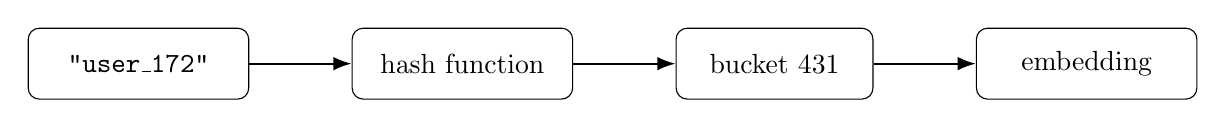
\begin{tikzpicture}[>=Latex, node distance=13mm, every node/.style={align=center}]
    \node[draw, rounded corners, minimum width=28mm, minimum height=9mm] (key) {\texttt{"user\_172"}};
    \node[draw, rounded corners, right=of key, minimum width=28mm, minimum height=9mm] (hash) {hash function};
    \node[draw, rounded corners, right=of hash, minimum width=25mm, minimum height=9mm] (bucket) {bucket 431};
    \node[draw, rounded corners, right=of bucket, minimum width=28mm, minimum height=9mm] (value) {embedding};
    \draw[->, thick] (key) -- (hash);
    \draw[->, thick] (hash) -- (bucket);
    \draw[->, thick] (bucket) -- (value);
    \end{tikzpicture}
    \caption{Conceptual hash-table lookup.}
    \label{fig:hash-map-flow}
\end{figure}

The goal is approximately
\[
    \underbrace{T_{\text{lookup}}}_{\text{lookup time}}
    \approx
    \underbrace{O(1)}_{\approx \text{independent of table size}}.
\]

Meaning the lookup does not normally become much slower just because you have millions of entries.

\textbf{Collision} may occur when two keys map to the same hash.


\begin{calloutintuition}
    Hash maps trade ordering for extremely fast exact lookup.
\end{calloutintuition}

A hash map assumes that you know the key exactly

\subsection{Trees: fast ordered lookup}
\label{subsec:trees-ordered-lookup}
Imagine sorted values:
\begin{center}
    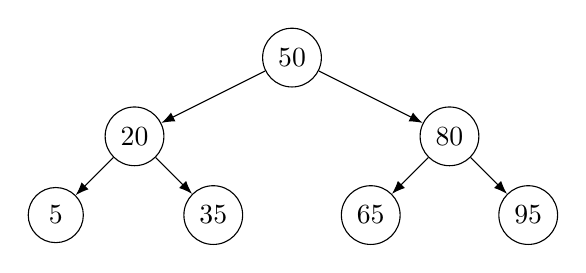
\begin{tikzpicture}[level distance=10mm, level 1/.style={sibling distance=40mm}, level 2/.style={sibling distance=20mm}, every node/.style={circle, draw, minimum size=7mm}, edge from parent/.style={draw,-Latex}]
    \node {50}
     child {node {20}
       child {node {5}}
       child {node {35}}
     }
     child {node {80}
       child {node {65}}
       child {node {95}}
     };
    \end{tikzpicture}
\end{center}
You eliminate large parts of the search space each step.
\[
    \underbrace{T_{\text{tree lookup}}}_{\text{lookup work}}
    \propto
    \log n
\]

% BOOK-LINK: If the tree-based models chapter discusses trees, explicitly distinguish
% algorithmic search trees from decision trees. The shared object is the recursive
% partitioning structure; the purpose is different.

\subsubsection{B-trees / B+ trees}
Binary trees are not ideal for disks because disk/database systems read data in blocks called \textbf{pages} and so databases usually prefer very wide trees.
\begin{center}
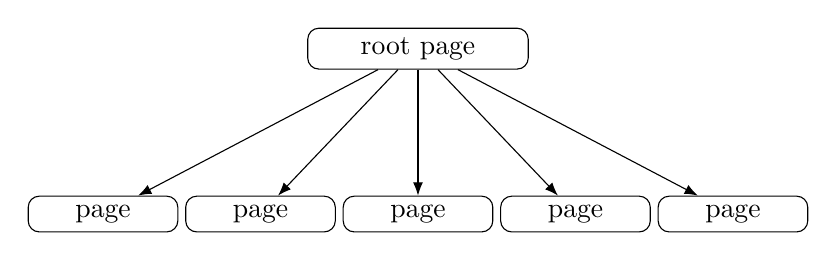
\begin{tikzpicture}[>=Latex, node distance=7mm and 8mm]
\node[draw, rounded corners, minimum width=28mm] (root) {root page};
\foreach \x/\name in {-4/p1,-2/p2,0/p3,2/p4,4/p5} {
  \node[draw, rounded corners, below=16mm of root, xshift=\x cm, minimum width=19mm] (\name) {page};
  \draw[->] (root) -- (\name);
}
\end{tikzpicture}
\end{center}

One page can contain many keys.
That reduces the number of storage accesses required.



\begin{calloutpracticaltip}
    A hash index is excellent for exact lookup.
    A tree index is excellent for ordered/range lookup.
\end{calloutpracticaltip}


\subsection{Queues}
\label{subsec:queues}

Suppose your CPU prepares training batches faster or slower than your GPU consumes them - the queue between them acts as a buffer.

\begin{figure}[htbp]
    \centering
    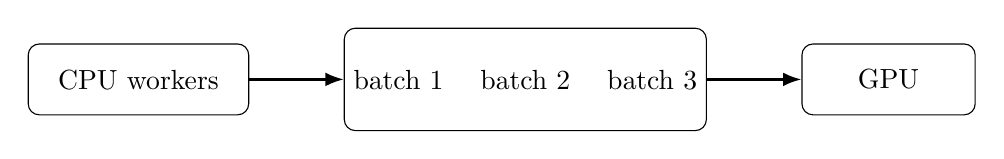
\begin{tikzpicture}[>=Latex, node distance=12mm]
    \node[draw, rounded corners, minimum width=28mm, minimum height=9mm] (cpu) {CPU workers};
    \node[draw, rounded corners, right=of cpu, minimum width=45mm, minimum height=13mm] (queue) {batch 1 \quad batch 2 \quad batch 3};
    \node[draw, rounded corners, right=of queue, minimum width=22mm, minimum height=9mm] (gpu) {GPU};
    \draw[->, thick] (cpu) -- (queue);
    \draw[->, thick] (queue) -- (gpu);
    \end{tikzpicture}
    \caption{A queue buffers work between a producer and a consumer.}
    \label{fig:producer-consumer-queue}
    \end{figure}
    Examples include:
    \begin{verbatim}
    DataLoader -> batch queue -> GPU
    web app -> job queue -> GPU inference worker
    event generator -> Kafka -> data pipeline
\end{verbatim}

The producer and consumer can run at different speeds, which is extremely useful. 

\paragraph{Backpressure}

Suppose rates $r_{\text{producer}} \gg r_{\text{consumer}}$, the queue grows by the difference.
Eventually a fix is needed, by: slowing producer, dropping data, increaseing  consumers, increasing buffering, fail
This is \textbf{backpressure}.
You will encounter this idea everywhere in distributed ML systems.

\subsection{Graphs and DAGs}
\label{subsec:graphs-dags}

A graph is a set of objects connected by relationships.
In ML systems, a particularly important version is a \textbf{directed acyclic graph} (DAG):

\begin{figure}[htbp]
\centering
\begin{tikzpicture}[>=Latex, node distance=10mm and 22mm, every node/.style={draw, rounded corners, align=center, minimum width=25mm, minimum height=8mm}]
\node (raw) {raw data};
\node[below=of raw] (clean) {clean};
\node[below left=of clean] (train) {train};
\node[below right=of clean] (val) {validation};
\node[below=of train] (model) {model};
\draw[->] (raw) -- (clean);
\draw[->] (clean) -- (train);
\draw[->] (clean) -- (val);
\draw[->] (train) -- (model);
\end{tikzpicture}
\caption{A DAG represents dependencies in a data or experiment pipeline.}
\label{fig:data-pipeline-dag}
\end{figure}

DAGs represent dependencies, from which workflow managers can say \textit{Step C cannot run until A and B are complete}.
You already implicitly use graphs when thinking about computational graphs, neural networks, data pipelines, and experiment dependencies.

% BOOK-LINK: Link this DAG discussion to the neural-network computational-graph section.

\section{Storage Hierarchy}
\label{sec:storage-hierarchy}

A computer has multiple storage levels.

\begin{figure}[htbp]
\centering
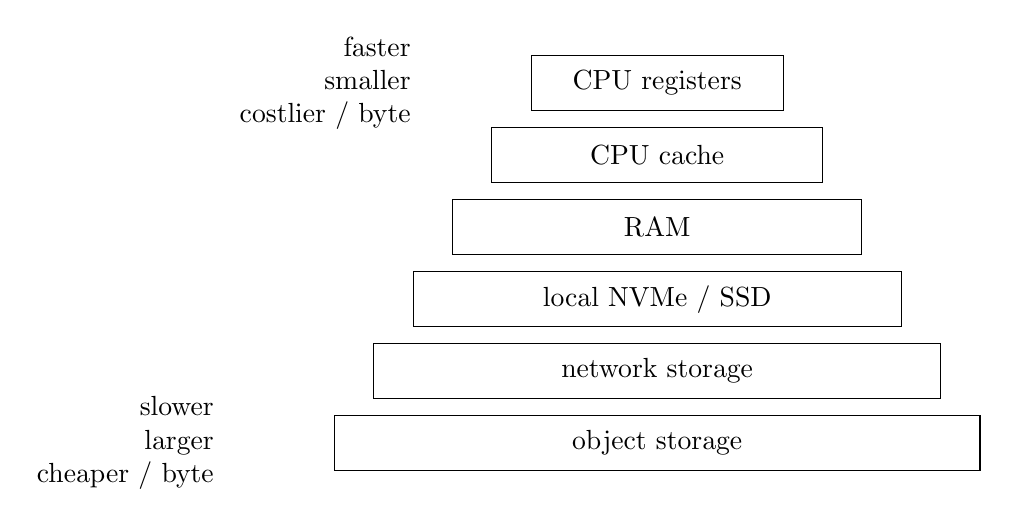
\begin{tikzpicture}[node distance=2mm, every node/.style={draw, minimum height=7mm, align=center}]
\node[minimum width=32mm] (reg) {CPU registers};
\node[below=of reg, minimum width=42mm] (cache) {CPU cache};
\node[below=of cache, minimum width=52mm] (ram) {RAM};
\node[below=of ram, minimum width=62mm] (ssd) {local NVMe / SSD};
\node[below=of ssd, minimum width=72mm] (net) {network storage};
\node[below=of net, minimum width=82mm] (obj) {object storage};
\node[left=14mm of reg, draw=none, align=right] {faster\\smaller\\costlier / byte};
\node[left=14mm of obj, draw=none, align=right] {slower\\larger\\cheaper / byte};
\end{tikzpicture}
\caption{Qualitative storage hierarchy. The exact ordering and performance numbers depend on hardware and workload, but the tradeoff direction is stable.}
\label{fig:storage-hierarchy}
\end{figure}

Usually, moving downward gives you more capacity, lower cost per byte, higher latency, and lower random-access performance.

\paragraph{Latency versus Bandwidth}
A system can have high latency and high bandwidth.
For example, opening a large remote object may be slow, but once transfer begins you may stream it quickly.
\begin{itemize}
    \item Latency: \textit{How long before you get the first result?}
    \item Bandwidth: \textit{How much data can you move per unit time?}
\end{itemize}


\subsection{Batching}
Assume that every requrest suffers some constant overhead cost, like $T_{\text{request}} = T_{\text{constant}} + T_{\text{variable}}$. 
Then, fetching one large block amortises it across a large dataset.
This appears in GPU matrix operations, database inserts, network calls, and disk reads.


\section{File Formats}
\label{sec:file-formats}

\subsection{CSV}

\begin{verbatim}
    name,age,height
    Alice,27,1.70
    Bob,34,1.83
\end{verbatim}

\begin{table}[h]
\centering
\begin{tabular}{p{0.45\linewidth} p{0.45\linewidth}}
\hline
\textbf{Advantages} & \textbf{Disadvantages} \\
\hline
Simple & Weak typing \\
Universal & Expensive parsing \\
Human-readable & Inefficient for large-scale analytics \\
 & Poor support for nested structure \\
\hline

\end{tabular}
\caption{Not necessarily ideal for large ML pipelines.}
\end{table}



\subsection{JSON}

\begin{verbatim}
{
  "user": 17,
  "features": {
    "country": "UK",
    "age": 24
  }
}
\end{verbatim}

Excellent when data is nested and flexible.
Common in APIs, configuration, logs, and metadata.
Less ideal for huge dense numerical arrays.

\subsection{NumPy \texttt{.npy}}
If your data is fundamentally an array, then storing it directly is much more natural.

\subsection{Row-oriented versus column-oriented storage}
\label{subsec:row-v-column}
A table contains [id | age | country | salary]:

\begin{figure}[h]
    \centering
    
    \begin{minipage}[t]{0.47\linewidth}
    \paragraph{Row orientation.}
    
    \begin{verbatim}
    [id1 age1 UK salary1]
    [id2 age2 US salary2]
    [id3 age3 FR salary3]
    \end{verbatim}
    
    \end{minipage}
    \hfill
    \begin{minipage}[t]{0.47\linewidth}
    \paragraph{Column orientation.}
    
    \begin{verbatim}
    [id1 id2 id3 ...]
    [age1 age2 age3 ...]
    [UK US FR ...]
    [salary1 salary2 salary3 ...]
    \end{verbatim}
    \end{minipage}
\end{figure}



\begin{figure}[htbp]
    \centering
    \resizebox{0.94\linewidth}{!}{%
    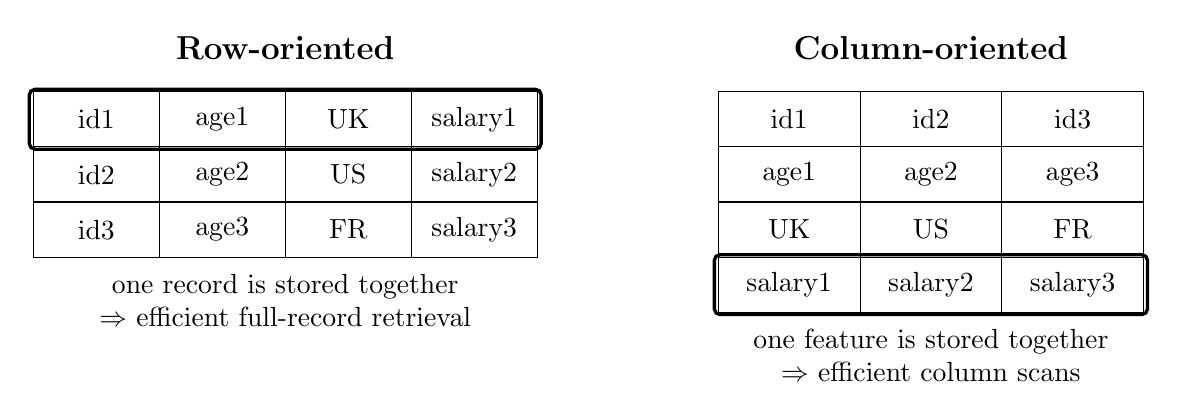
\begin{tikzpicture}[
        >=Latex,
        cell/.style={
            draw,
            minimum width=1.6cm,
            minimum height=0.7cm,
            inner sep=0pt
        },
        highlight/.style={
            draw,
            very thick,
            rounded corners=2pt
        }
    ]
    
    % =========================================================
    % Row-oriented layout
    % =========================================================
    \begin{scope}
    
    \node[font=\bfseries\large] at (3.2,3.25) {Row-oriented};
    
    % Grid
    \foreach \r in {0,...,2} {
        \foreach \c in {0,...,3} {
            \node[cell] at ({0.8 + 1.6*\c},{2.35 - 0.7*\r}) {};
        }
    }
    
    % Values
    \node at (0.8,2.35) {id1};
    \node at (2.4,2.35) {age1};
    \node at (4.0,2.35) {UK};
    \node at (5.6,2.35) {salary1};
    
    \node at (0.8,1.65) {id2};
    \node at (2.4,1.65) {age2};
    \node at (4.0,1.65) {US};
    \node at (5.6,1.65) {salary2};
    
    \node at (0.8,0.95) {id3};
    \node at (2.4,0.95) {age3};
    \node at (4.0,0.95) {FR};
    \node at (5.6,0.95) {salary3};
    
    % Highlight one complete record
    \draw[highlight]
        (-0.05,1.97) rectangle (6.45,2.73);
    
    \node[align=center] at (3.2,0.05)
        {one record is stored together\\
         $\Rightarrow$ efficient full-record retrieval};
    
    \end{scope}
    
    
    % =========================================================
    % Column-oriented layout
    % =========================================================
    \begin{scope}[xshift=8.7cm]
    
    \node[font=\bfseries\large] at (2.7,3.25) {Column-oriented};
    
    % Grid
    \foreach \r in {0,...,3} {
        \foreach \c in {0,...,2} {
            \node[
                draw,
                minimum width=1.8cm,
                minimum height=0.7cm,
                inner sep=0pt
            ] at ({0.9 + 1.8*\c},{2.35 - 0.7*\r}) {};
        }
    }
    
    % Values
    \node at (0.9,2.35) {id1};
    \node at (2.7,2.35) {id2};
    \node at (4.5,2.35) {id3};
    
    \node at (0.9,1.65) {age1};
    \node at (2.7,1.65) {age2};
    \node at (4.5,1.65) {age3};
    
    \node at (0.9,0.95) {UK};
    \node at (2.7,0.95) {US};
    \node at (4.5,0.95) {FR};
    
    \node at (0.9,0.25) {salary1};
    \node at (2.7,0.25) {salary2};
    \node at (4.5,0.25) {salary3};
    
    % Highlight one complete logical column
    % (salary values are physically contiguous)
    \draw[highlight]
        (-0.05,-0.13) rectangle (5.45,0.63);
    
    \node[align=center] at (2.7,-0.65)
        {one feature is stored together\\
         $\Rightarrow$ efficient column scans};
    
    \end{scope}
    
    \end{tikzpicture}%
    }
    
    \caption{The same logical table can be laid out to favour full-record access or column-wise scans.}
    \label{fig:row-v-column}
\end{figure}

\subsection{Parquet}

Parquet is a major format for large structured datasets.
Its inductive bias is large analytical tabular workloads.
Strengths: [columnar, typed, compressed, chunk metadata and can avoid reading irrelevant columns.

Suppose your table has 100 columns, but your experiment only needs \texttt{user\_id}, \texttt{label}, and \texttt{embedding}.
A columnar system may avoid reading the other 97 which is a huge win.

\subsection{Arrow}

Apache Arrow is a standardised \textbf{columnar memory representation}.
Think of Pandas, Polars, Spark, databases, and ML systems all wanting to exchange structured data without constantly serialising and reparsing everything.
Arrow helps define a common representation between them all.


\begin{table}[htbp]
\centering
\caption{Common data formats and their useful mental models.}
\label{tab:data-formats}
\begin{tabularx}{\linewidth}{@{}lXX@{}}
\toprule
\textbf{Format} & \textbf{Mental model} & \textbf{Typical use} \\
\midrule
CSV & Human-readable rows of text & Simple interchange, small tables \\
JSON & Flexible nested records & APIs, metadata, logs, configuration \\
NumPy \texttt{.npy} & Typed numerical array & Scientific arrays, local experiments \\
HDF5 & Structured numerical container & Scientific computing and large array collections \\
Parquet & Compressed columnar table & Large analytical datasets \\
Arrow & In-memory columnar representation & Fast interchange between analytical tools \\
Tar/WebDataset-style shards & Many samples packed into larger sequential objects & Large-scale ML dataset streaming \\
\bottomrule
\end{tabularx}
\end{table}

\section{Relational Databases}
\label{sec:relational-databases}

The relational model thinks in tables.

\begin{center}
    \begin{tabular}{@{}rrrrr@{}}
    \toprule
    id & model\_id & dataset\_id & lr & accuracy \\
    \midrule
    1 & 17 & 3 & $10^{-4}$ & 0.912 \\
    2 & 21 & 3 & $3\times10^{-4}$ & 0.887 \\
    \bottomrule
    \end{tabular}
\end{center}

Another table:

\begin{center}
    \begin{tabular}{@{}rl@{}}
    \toprule
    id & name \\
    \midrule
    17 & ViT-B \\
    21 & ResNet \\
    \bottomrule
    \end{tabular}
\end{center}

A \textbf{Primary key} uniquely identifies a row, and a \textbf{Foreign key} maps between entries.

Suppose \texttt{experiments.model\_id = 17} and \texttt{models.id = 17}.
The first points at the second.

\begin{center}
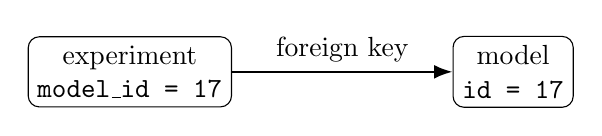
\begin{tikzpicture}[>=Latex, node distance=28mm]
\node[draw, rounded corners, align=center] (exp) {experiment\\\texttt{model\_id = 17}};
\node[draw, rounded corners, align=center, right=of exp] (model) {model\\\texttt{id = 17}};
\draw[->, thick] (exp) -- node[above]{foreign key} (model);
\end{tikzpicture}
\end{center}

That gives you relationships between entities.

\subsubsection{Joins}

Suppose experiments store \texttt{model\_id}, but model names live elsewhere.
A join combines them.

\begin{verbatim}
    SELECT experiments.id, models.name
    FROM experiments
    JOIN models
    ON experiments.model_id = models.id;
\end{verbatim}

Conceptually, an experiment row with \texttt{model\_id = 17} connects to the model row with \texttt{id = 17} and \texttt{name = ViT}.

\subsubsection{Normalisation}

Suppose you store:

\begin{verbatim}
    experiment 1 | dataset_name="ImageNet" | dataset_path=...
    experiment 2 | dataset_name="ImageNet" | dataset_path=...
    experiment 3 | dataset_name="ImageNet" | dataset_path=...
\end{verbatim}

You have duplicated information.
Instead, experiments can store a \texttt{dataset\_id} that points to one canonical datasets table.
The tradeoff is between duplication and more joins vs deduplicated and no joins.

\section{Indexes}
\label{sec:database-indexes}

Finding an element normally requires to search, which is expensive.
With an index, the database maintains an auxiliary structure between index and row location, such that lookup is much faster.

An index is not free, because every time you insert a new row, you may also need to update index 1, index 2, index 3, and so on, meaning that
\[
\text{more indexes}
\Rightarrow
\text{faster selected reads}
+
\text{more storage}
+
\text{more expensive writes}
.
\]
You may also compose indexes of many columns, at additional cost, known as \textbf{composite indexes}.

\section{Transactions and Concurrency}
\label{sec:transactions-concurrency}
Suppose a bank transfer requires:
\begin{verbatim}
    subtract £10 from Alice
    add £10 to Bob
\end{verbatim}
If the system crashes after the first operation, the database is inconsistent.
You want the two operations to behave as one logical unit of subtract, add then commit, such that either both happen or neither happens.

\subsection{ACID}
\begin{itemize}
    \item \textbf{Atomicity.} All-or-nothing.
    \item \textbf{Consistency.} Database rules remain valid.
    \item \textbf{Isolation.} Concurrent operations should not interfere in surprising ways.
    \item \textbf{Durability.} After a successful commit, a crash should not casually erase the result.
\end{itemize}

\subsection{Race conditions}

Suppose a shared counter is 10.
Then, machine A reads 10 and adds 1 and machine B reads 10 and adds 1.
Both write 11, but the expected result is 12
Concurrency is why databases need things such as locks, transactions and versioning.

\section{Caches}
\label{sec:caches}
A cache stores a fast temporary copy of data, this is expensive to fetch or compute repeatedly.
Think of it as
\[
\underbrace{\text{repeated request}}_{\text{same or recently used data}}
\rightarrow
\underbrace{\text{fast copy}}_{\text{cache}}
\rightarrow
\underbrace{\text{slow source only on a miss}}_{\text{database / object store / computation}}.
\]

\begin{figure}[htbp]
\centering
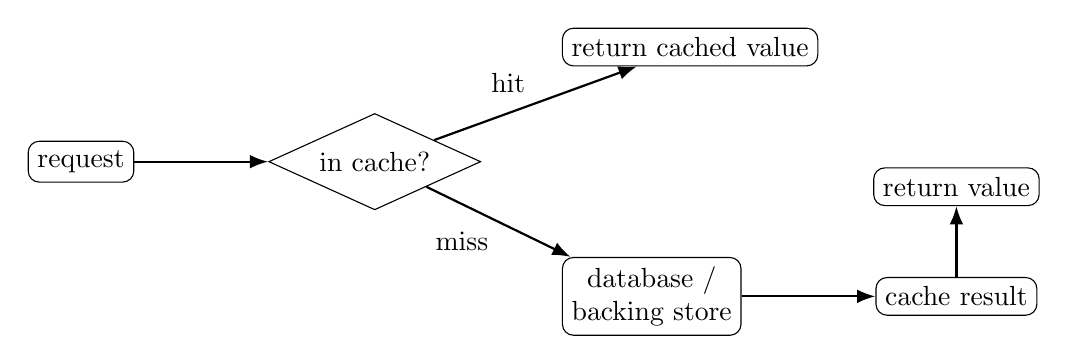
\begin{tikzpicture}[>=Latex, node distance=9mm and 17mm, every node/.style={align=center}]
\node[draw, rounded corners] (request) {request};
\node[draw, diamond, aspect=2.2, right=of request] (cache) {in cache?};
\node[draw, rounded corners, above right=of cache] (hit) {return cached value};
\node[draw, rounded corners, below right=of cache] (db) {database /\\backing store};
\node[draw, rounded corners, right=of db] (fill) {cache result};
\node[draw, rounded corners, above=of fill] (return) {return value};
\draw[->, thick] (request) -- (cache);
\draw[->, thick] (cache) -- node[above left]{hit} (hit);
\draw[->, thick] (cache) -- node[below left]{miss} (db);
\draw[->, thick] (db) -- (fill);
\draw[->, thick] (fill) -- (return);
\end{tikzpicture}
\caption{Cache-aside access: repeated requests are served from the fast copy; misses fall through to the backing store and refill the cache.}
\label{fig:cache-aside-overview}
\end{figure}

Caching exploits \textbf{temporal locality} by assuming that recently/frequent values are likely to be requested again.
\textbf{Spatial locality} is the related idea that nearby values are often accessed together, which is more important for CPU caches, arrays, and storage blocks than for a typical Redis key lookup.

Let the cache hit rate be $h$ and a cache lookup cost \(L_c\). 
A miss requires a full lookup costing \(L_b\) and so when designing a cache we must balance speed and hit rate through the cache size. 

\subsection{Redis}
\label{subsec:redis}

Redis can be treated conceptually as a fast, network-accessible, in-memory data-structure store, kind of like a python \textsc{dict} but globally accessible (rather than within a python process) to many downstream users or services.
Redis Cluster shards by: a key maps to a slot and the slot maps to the node responsible for it.
The partition/sharding function matters because uneven traffic can create a \textbf{hot shard}: one machine receives a disproportionate amount of storage, requests, or compute.

Its natural bias is exact-key access:
\[
    \underbrace{\texttt{user:127}}_{\text{known key}}
    \rightarrow
    \underbrace{\text{embedding / profile / state}}_{\text{small value}}.
\]
\textbf{Time to Live (TTL)} adds a tame based expiry to a cache entry, reducing staleness at the sacrifice of additional compute (and removal of potential cache hits).

\textbf{Cache Invalidation} causes misalignment between cache and underlying database, known as staleness.

\textbf{Eviction Policies} decide how to reduce the cache entry count when maximum memory is reached.
Examples are \textit{query frequency}, \textit{item size} may be used to make the decision. 
% <TODO>: Link cache locality back to the earlier memory-locality discussion.

\begin{calloutintuition}
    Caches duplicate the data into a easy-query format like in-RAM or lookup-table.
\end{calloutintuition}

\begin{table}[htbp]
    \centering
    \caption{Some use cases of Redis style caches, and why.}
    \label{tab:redis-use-cases}
    \begin{tabularx}{\linewidth}{@{}lXX@{}}
    \toprule
    \textbf{Use} & \textbf{Access pattern} & \textbf{Why it fits} \\
    \midrule
    Cache & key \(\rightarrow\) reused result & avoids repeated slower work \\
    Session state & session ID \(\rightarrow\) state & fast shared lookup across application servers \\
    Feature lookup & entity ID \(\rightarrow\) features & low-latency inference input \\
    Rate limit & key \(\rightarrow\) counter & cheap updates with expiry \\
    Leaderboard & member \(\leftrightarrow\) score & sorted data structures support ranking \\
    Temporary state & key \(\rightarrow\) short-lived value & expiration is a first-class operation \\
    \bottomrule
    \end{tabularx}
\end{table}


\section{Distributed Storage}
\label{sec:redis-cluster}
\label{sec:replication-v-sharding}
\label{sec:distributed-consistency}

Distributed storage applies a \textbf{divide} or \textbf{copy} state across machines.

\subsection{Sharding}
Split the keyspace into shards:

\begin{figure}[htbp]
    \centering
    \caption{Sharding}
    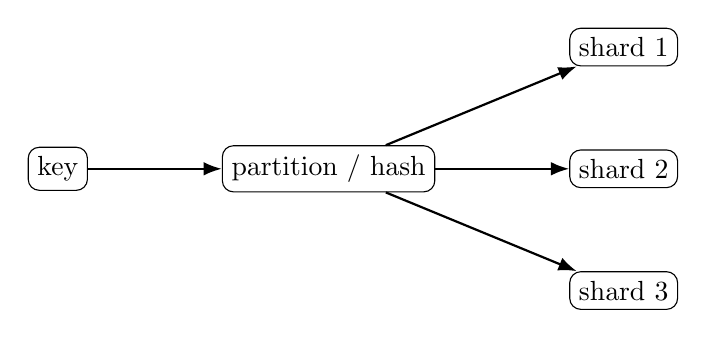
\begin{tikzpicture}[>=Latex, node distance=10mm and 17mm, every node/.style={align=center}]
    \node[draw, rounded corners] (key) {key};
    \node[draw, rounded corners, right=of key] (hash) {partition / hash};
    \node[draw, rounded corners, above right=of hash] (s1) {shard 1};
    \node[draw, rounded corners, right=of hash] (s2) {shard 2};
    \node[draw, rounded corners, below right=of hash] (s3) {shard 3};
    \draw[->, thick] (key) -- (hash);
    \draw[->, thick] (hash) -- (s1);
    \draw[->, thick] (hash) -- (s2);
    \draw[->, thick] (hash) -- (s3);
    \end{tikzpicture}
\end{figure}

\subsection{Replication}
Replication stores additional copies of the same state:

\begin{figure}[htbp]
    \centering
    \caption{Replication}
    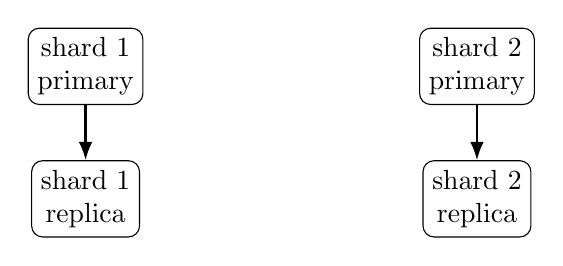
\begin{tikzpicture}[>=Latex, node distance=7mm and 20mm, every node/.style={align=center}]
    \node[draw, rounded corners] (p1) {shard 1\\primary};
    \node[draw, rounded corners, below=of p1] (r1) {shard 1\\replica};
    \node[draw, rounded corners, right=35mm of p1] (p2) {shard 2\\primary};
    \node[draw, rounded corners, below=of p2] (r2) {shard 2\\replica};
    \draw[->, thick] (p1) -- (r1);
    \draw[->, thick] (p2) -- (r2);
    \end{tikzpicture}
    \caption{Large systems commonly combine sharding, which divides state, with replication, which copies each shard for availability or additional reads.}
    \label{fig:replication-plus-sharding}
\end{figure}

\begin{table}[htbp]
    \centering
    \begin{tabularx}{\linewidth}{@{}lXX@{}}
    \toprule
     & \textbf{Primary purpose} & \textbf{New problem introduced} \\
    \midrule
    Sharding & capacity and aggregate throughput & partition choice, rebalancing, hot shards \\
    Replication & availability and sometimes read throughput & replica lag, failover, consistency \\
    \bottomrule
    \end{tabularx}
\end{table}

\subsection{Consistency}
The moment data is replicated, different machines can temporarily disagree.
For example, A write may reach the primary before every replica.
\begin{itemize}
    \item \textbf{Strong Consistency:} Minimise staleness through large communication. Downstream logic assumes no staleness. 
    \item \textbf{Eventual Consistency:} Balance staleness with communication. Downstream logic/Applications must handle stale reads.
\end{itemize}

\begin{calloutpractical}
    When choosing a consistency model, ask what incorrect behaviour a stale read would actually cause.
\end{calloutpractical}



\section{Database Families}
\label{sec:database-families}

\begin{table}[htbp]
    \centering
    \caption{Database Families}
    \label{tab:database-families}
    \begin{tabularx}{\linewidth}{@{}lXXX@{}}
    \toprule
    \textbf{Family} & \textbf{Structural bias} & \textbf{Natural query} & \textbf{Typical use} \\
    \midrule
    Relational & structured entities and relations & filters, joins, transactions & users, experiments, jobs, metadata \\
    Key--value & exact key is known & key \(\rightarrow\) value & caches, sessions, entity lookup \\
    Document & one entity has flexible nested structure & load/filter documents & semi-structured application state \\
    Columnar / analytical & queries scan few columns over many rows & aggregate / group / scan & analytics and warehouses \\
    Time-series & measurements are organised by time & range by timestamp & metrics and monitoring \\
    Graph & relationships are first-class & traverse neighbours / paths & relationship-heavy domains \\
    Vector & similarity maps to geometric proximity & nearest neighbours & semantic retrieval \\
    \bottomrule
    \end{tabularx}
\end{table}


\section{Vector Databases}
\label{sec:vector-databases}
Key based databases store exact one-to-one/many values. 
Vector databases drop values into a vector space and allow representation queries like \textit{Give me items who are close to value Y}. 
Where \textit{value Y} is a vector, this means a cosine difference. 
In practice, use nearest-neighbour search (or approximate-nearest-neighbour) and balance $k$ with dataset size and recall requirements.
One perspective of a vector database is to imagine the dataset as a matrix, and multiply the matrix by the query - the weighting is the cosine difference and you pick the top $k$. 
In practice it is harder because of data sizes.
The design variables are the embedding model, similarity measure, index family and parameters, search depth, retrieved \(k\), and any metadata filters.

\subsection{Retrieval-Augmented Generation}
Vector retrieval commonly appears inside RAG.

\begin{figure}[htbp]
\centering
\resizebox{0.96\linewidth}{!}{%
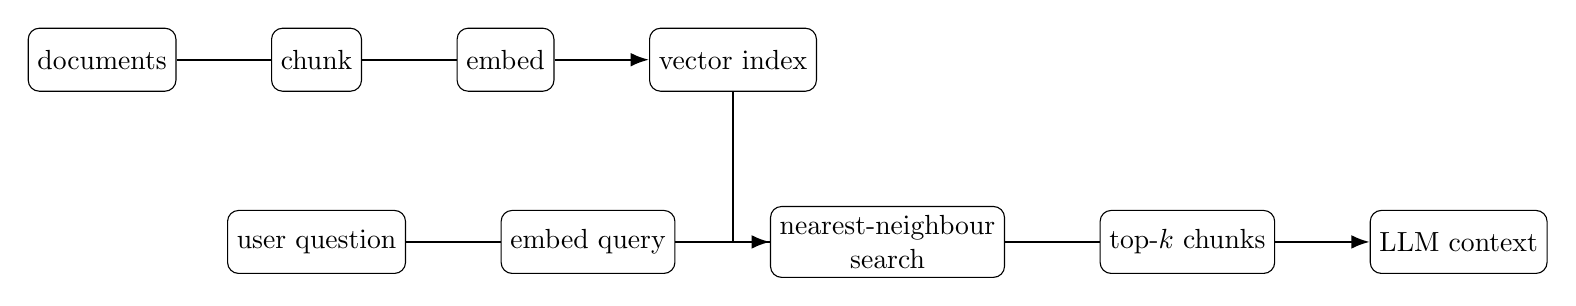
\begin{tikzpicture}[>=Latex, node distance=8mm and 12mm, every node/.style={draw, rounded corners, align=center, minimum height=8mm}]
\node (docs) {documents};
\node[right=of docs] (chunk) {chunk};
\node[right=of chunk] (embed) {embed};
\node[right=of embed] (index) {vector index};
\node[below=15mm of chunk] (question) {user question};
\node[right=of question] (qembed) {embed query};
\node[right=of qembed] (search) {nearest-neighbour\\search};
\node[right=of search] (topk) {top-\(k\) chunks};
\node[right=of topk] (llm) {LLM context};
\draw[->, thick] (docs)--(chunk)--(embed)--(index);
\draw[->, thick] (question)--(qembed)--(search)--(topk)--(llm);
\draw[->, thick] (index) |- (search);
\end{tikzpicture}%
}
\caption{RAG separates document indexing from query-time retrieval; chunking, embedding, ANN search, metadata filtering, and reranking are all experimental degrees of freedom.}
\label{fig:rag-data-flow}
\end{figure}

% TODO: Link cosine similarity and embedding geometry to the embeddings/LLM chapter.

\section{Object Storage and Lakehouses}
\label{sec:object-storage}
\label{sec:data-lakes-lakehouses}

Data has two structures:
\begin{itemize}
    \item \textbf{Structured:} Tables, Databases. Stored in \textit{Data Warehouses}. 
    \item \textbf{UnStructured:} Large Files, non-tabular etc. Stored in \textit{Data Lakes}.
\end{itemize}
We mix these structures into a \textit{Lakehouse}, a structrued store of unstructured data. 
Imagine a Video Streaming database where each metadata column (name, upload date, \dots) is a column, and there exists another column of 'content' which contains either the video data itself.
If instead that content stored a relational-database key, this structure would be a data warehouse with a relational link to a data lake - we prefer a unified approach.

Large ML datasets and checkpoints often live in this object storage such as S3/GCS because capacity, durability, and access from many compute workers matter more than local-filesystem semantics.
The interface is conceptually object-oriented with commands: [$\texttt{PUT object},\qquad \texttt{GET object},\qquad \texttt{DELETE object}$], rather than arbitrary cheap in-place edits to remote files.

This enables \textbf{compute--storage separation}: training clusters can be created or destroyed independently while the dataset persists in shared durable storage.
The tradeoff is that remote object access has higher latency than local RAM or SSD, so large sequential reads, dataset sharding, prefetching, and local caches are usually preferable to millions of tiny random object requests.

\section{ML Data Pipelines}
\label{sec:training-data-pipeline}
\label{sec:online-inference-data}

\subsection{Training}
Pulling this all together, training requires passing data a thinning stream. 
Speed increases in each stage, but memory falls, and so we utilise parallel processing.
It is often efficient to conduct data preprocessing, and augmentation in these stages. 

\begin{figure}[htbp]
\centering
\resizebox{0.98\linewidth}{!}{%
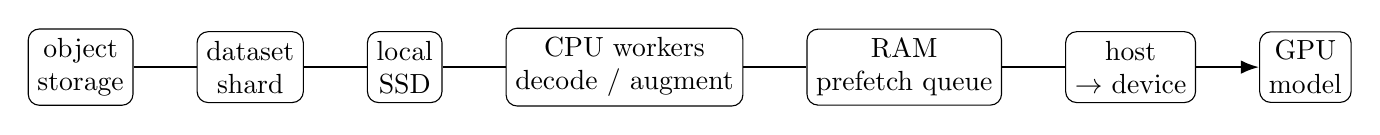
\begin{tikzpicture}[>=Latex, node distance=5mm and 8mm, every node/.style={draw, rounded corners, align=center, minimum height=8mm}]
\node (obj) {object\\storage};
\node[right=of obj] (shard) {dataset\\shard};
\node[right=of shard] (ssd) {local\\SSD};
\node[right=of ssd] (cpu) {CPU workers\\decode / augment};
\node[right=of cpu] (queue) {RAM\\prefetch queue};
\node[right=of queue] (copy) {host\\$\rightarrow$ device};
\node[right=of copy] (gpu) {GPU\\model};
\draw[->, thick] (obj)--(shard)--(ssd)--(cpu)--(queue)--(copy)--(gpu);
\end{tikzpicture}%
}
\caption{The training path is a pipeline of increasing speed and decreasing memory, ending at the training GPU's.}
\label{fig:training-input-path}
\end{figure}

\textbf{Prefetching} overlaps GPU computation with batch-preparation, because if preparing the next batch takes longer than GPU computation, the GPU becomes \textbf{input-starved}.

\begin{figure}[htbp]
\centering
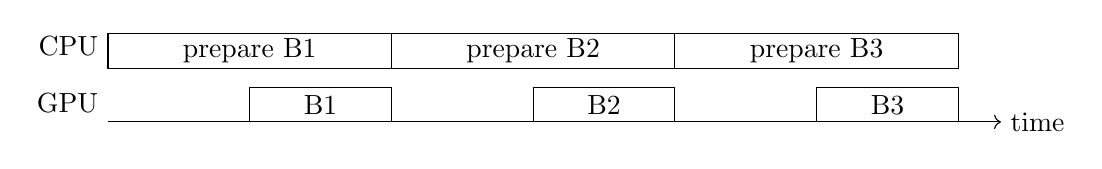
\begin{tikzpicture}[x=18mm,y=8mm]
\draw[->] (0,0) -- (6.3,0) node[right]{time};
\node[left] at (0,1.2) {CPU};
\node[left] at (0,0.3) {GPU};
\foreach \x/\lab in {0/B1,2/B2,4/B3} {
  \draw (\x,0.85) rectangle ++(2,0.55) node[midway]{prepare \lab};
}
\foreach \x/\lab in {1/B1,3/B2,5/B3} {
  \draw (\x,0.0) rectangle ++(1,0.55) node[midway]{\lab};
}
\end{tikzpicture}
\caption{Prefetching overlaps CPU preparation of batch \(n+1\) with GPU computation on batch \(n\).}
\label{fig:prefetching-overlap}
\end{figure}

Increasing workers helps only until another resource becomes limiting; the bottleneck may migrate from CPU decode to disk, network, memory bandwidth, host-to-device transfer, or finally model compute.

\subsection{Online inference}
Serving usually cares more about request latency and tail latency than raw samples/s.

\begin{figure}[htbp]
\centering
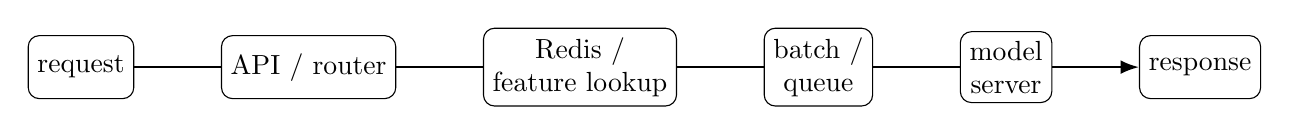
\begin{tikzpicture}[>=Latex, node distance=8mm and 11mm, every node/.style={draw, rounded corners, align=center, minimum height=8mm}]
\node (req) {request};
\node[right=of req] (api) {API / router};
\node[right=of api] (feature) {Redis /\\feature lookup};
\node[right=of feature] (queue) {batch /\\queue};
\node[right=of queue] (model) {model\\server};
\node[right=of model] (resp) {response};
\draw[->, thick] (req)--(api)--(feature)--(queue)--(model)--(resp);
\end{tikzpicture}
\caption{End-to-end serving latency contains infrastructure and data-access costs in addition to neural-network compute.}
\label{fig:inference-request-path}
\end{figure}

A useful decomposition is
\[
\underbrace{L_{\text{total}}}_{\text{request latency}}
\approx
\underbrace{L_{\text{network}}}_{\text{transport}}
+
\underbrace{L_{\text{lookup}}}_{\text{features / state}}
+
\underbrace{L_{\text{queue}}}_{\text{waiting}}
+
\underbrace{L_{\text{model}}}_{\text{inference}}
+
\underbrace{L_{\text{post}}}_{\text{post-processing}}.
\]
Optimising a 20 ms model is low leverage if another stage contributes 150 ms.

Tail metrics such as \(p_{95}\) and \(p_{99}\) expose rare slow requests hidden by a good mean.
\textbf{Dynamic batching} waits briefly to combine requests into a GPU-efficient batch, trading some per-request latency for higher accelerator throughput.

% BOOK-LINK: Link training throughput to batching/distributed training and serving latency to the inference chapter.


\section{Performance Arithmetic}
\label{sec:performance-arithmetic}
\label{sec:system-design-optimisation}
\label{sec:data-system-optionality}

Back-of-the-envelope arithmetic is often enough to identify an impossible architecture before profiling it.
If decoded samples have size \(D_s\), each batch contains \(B\) samples, and the accelerator consumes \(r_b\) batches/s, then
\[
\underbrace{\dot D_{\text{required}}}_{\text{required input bandwidth}}
=
\underbrace{D_s}_{\text{bytes / sample}}
\times
\underbrace{B}_{\text{samples / batch}}
\times
\underbrace{r_b}_{\text{batches / second}}.
\]
For \(D_s=2\) MB, \(B=256\), and \(r_b=4\), the data path must sustain roughly 2 GB/s after decoding.
A storage path supplying 0.5 GB/s cannot keep that workload fed regardless of model optimisation.


\begin{table}[htbp]
\centering
\caption{Qualitative tradeoffs of common layers.}
\label{tab:storage-tradeoffs}
\begin{tabularx}{\linewidth}{@{}lXXXX@{}}
\toprule
\textbf{Layer} & \textbf{Latency} & \textbf{Capacity} & \textbf{Durability} & \textbf{Natural role} \\
\midrule
GPU memory & extremely low & small & low & active tensors / model state \\
CPU RAM & low & moderate & low & working set / preprocessing \\
Local SSD & moderate & large & machine-local & dataset/cache staging \\
Redis & low network lookup & RAM-limited / sharded & configuration-dependent & hot shared state / cache \\
Relational DB & moderate & large & strong & structured canonical state \\
Object storage & high per-access & very large & high & durable datasets / checkpoints \\
\bottomrule
\end{tabularx}
\end{table}

Choosing a system based on the task:
\begin{itemize}
    \item Small experiment metadata on one machine \(\rightarrow\) files or SQLite.
    \item Concurrent structured state and flexible queries \(\rightarrow\) relational database.
    \item Repeated low-latency \(\text{entity ID}\rightarrow\text{feature}\) access \(\rightarrow\) Redis-like cache/key--value storage.
    \item Multi-terabyte or petabyte training corpora \(\rightarrow\) object storage plus sharded files.
    \item Semantic similarity search \(\rightarrow\) a vector index.
\end{itemize}

\section{Overview}
\label{sec:data-systems-evolution}
\label{sec:inductive-bias-data-systems}

\begin{table}[htbp]
\centering
\caption{Useful memory model: each component encodes an access-pattern bias.}
\label{tab:inductive-bias-data-systems}
\begin{tabularx}{\linewidth}{@{}lX@{}}
\toprule
\textbf{Technology} & \textbf{Structural assumption / inductive bias} \\
\midrule
Array & data is regularly indexed and numerical \\
Hash map & exact key identity is known \\
Tree index & ordering and range queries matter \\
Queue & producer and consumer rates should be decoupled \\
Relational DB & structured entities and relationships matter \\
Redis / cache & low-latency repeated key-based access matters \\
Parquet / columnar store & scans touch subsets of columns over many rows \\
Object store & large durable objects can be accessed remotely \\
Kafka-like log & data is an ordered replayable event stream \\
Vector index & semantic similarity maps to geometric proximity \\
Sharding & workload can be partitioned across machines \\
Replication & duplicate copies improve availability/read capacity \\
\bottomrule
\end{tabularx}
\end{table}


\begin{figure}[htbp]
\centering
\resizebox{0.88\linewidth}{!}{%
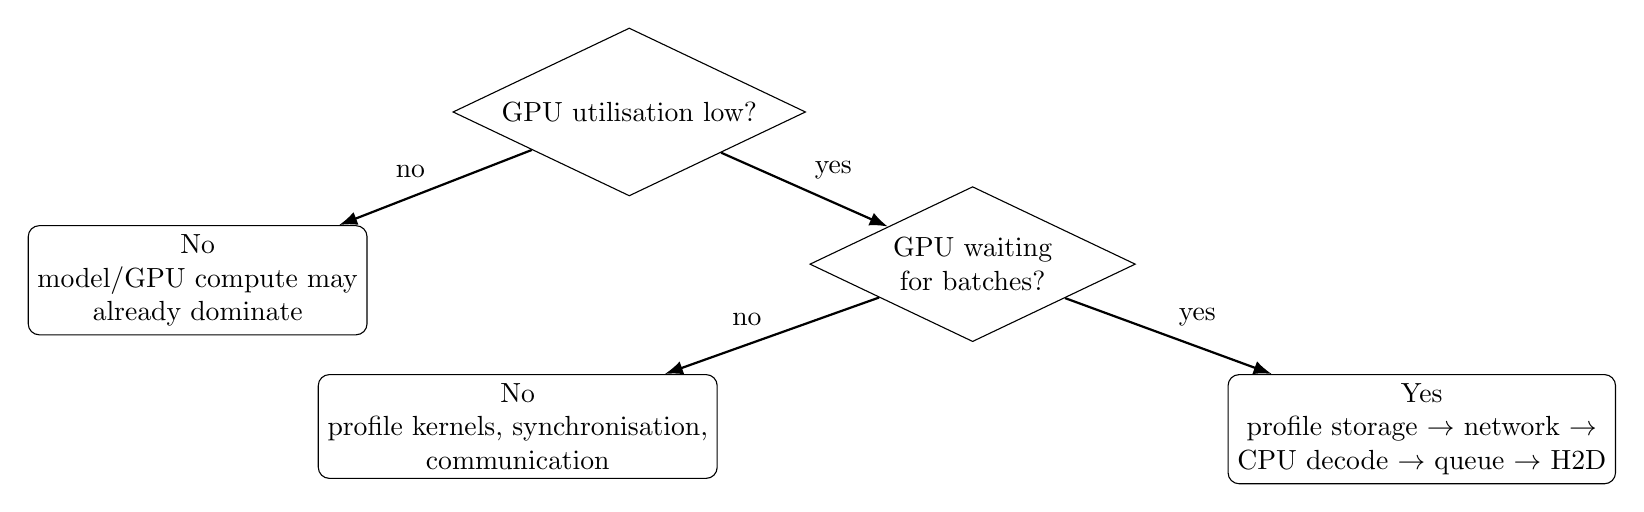
\begin{tikzpicture}[>=Latex, node distance=9mm and 22mm, every node/.style={align=center}]
\node[draw, diamond, aspect=2.1] (low) {GPU utilisation low?};
\node[draw, rounded corners, below left=of low] (compute) {No\\model/GPU compute may\\already dominate};
\node[draw, diamond, aspect=2.1, below right=of low] (wait) {GPU waiting\\for batches?};
\node[draw, rounded corners, below left=of wait] (other) {No\\profile kernels, synchronisation,\\communication};
\node[draw, rounded corners, below right=of wait] (path) {Yes\\profile storage $\rightarrow$ network $\rightarrow$\\CPU decode $\rightarrow$ queue $\rightarrow$ H2D};
\draw[->, thick] (low)--node[above left]{no}(compute);
\draw[->, thick] (low)--node[above right]{yes}(wait);
\draw[->, thick] (wait)--node[above left]{no}(other);
\draw[->, thick] (wait)--node[above right]{yes}(path);
\end{tikzpicture}%
}
\caption{A diagnostic tree for separating model-compute bottlenecks from input-pipeline bottlenecks.}
\label{fig:training-diagnostic-tree}
\end{figure}

A Redis-backed inference example follows the same reasoning: if requests repeatedly need \(\texttt{user\_id}\rightarrow\text{embedding}\), an in-memory shared cache matches the access pattern; when one node becomes too small, shard the keys; when node loss becomes unacceptable, replicate the shards; once copies exist, consistency and invalidation become explicit design problems.
\chapter{Foundations: Hardware}
\label{sec:hardware}

Hardware issues are normally about\textbf{where work happens, where bytes move, and what waits for what}, because compute is surrounded by memory, launch overheads, scheduling and synchronising. 

\[
    \underbrace{T_{\text{step}}}_{\text{wall-clock step time}}
    &\approx
    \underbrace{T_{\text{exposed compute}}}_{\text{arithmetic on critical path}}
    +
    \underbrace{T_{\text{exposed memory}}}_{\text{local movement}}
    \quad+
    \underbrace{T_{\text{exposed communication}}}_{\text{GPU / node movement}}
    +
    \underbrace{T_{\text{launch + queue + sync}}}_{\text{coordination}}.
\]

Summing the raw duration of every kernel, copy, and collective can overestimate wall-clock time by ignoring overlapping work.

\begin{figure}[H]
\centering
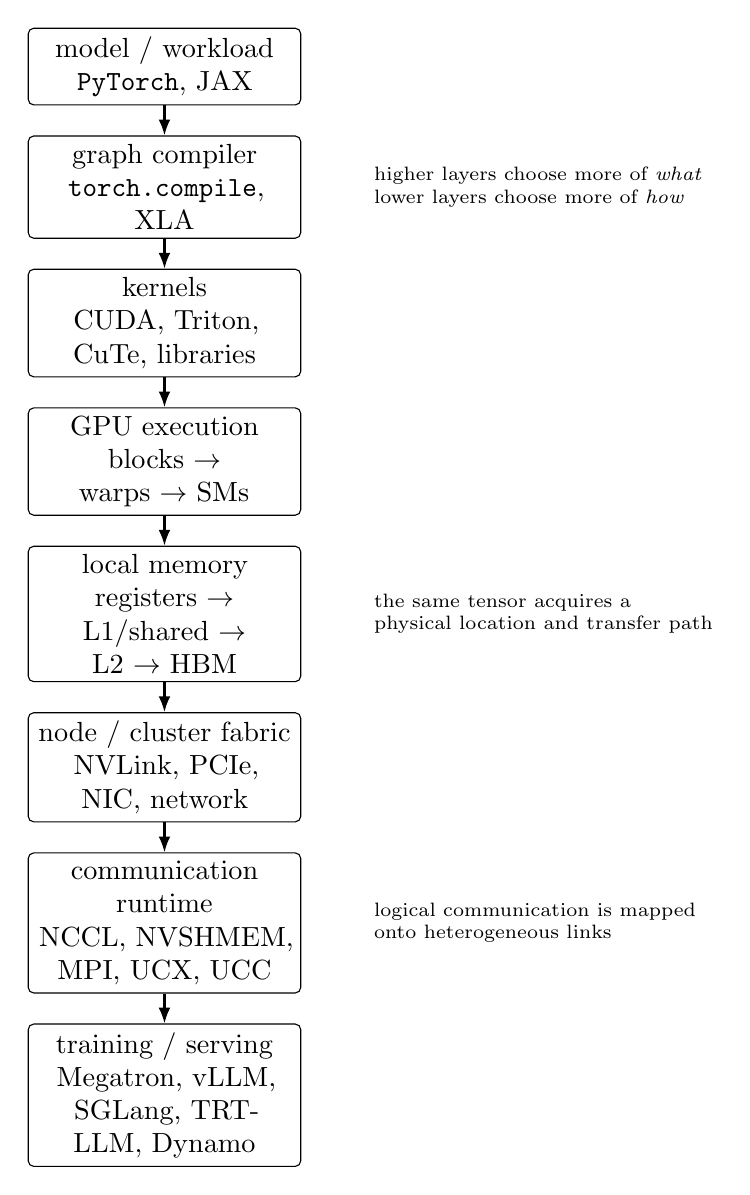
\begin{tikzpicture}[
  node distance=3.8mm and 7mm,
  box/.style={draw, rounded corners=2pt, minimum height=7.5mm, text width=3.25cm, align=center, inner sep=3pt},
  arr/.style={-{Latex[length=2mm]}, thick},
  lab/.style={font=\scriptsize, align=left}
]
\node[box] (model) {model / workload\\\texttt{PyTorch}, JAX};
\node[box, below=of model] (compiler) {graph compiler\\\texttt{torch.compile}, XLA};
\node[box, below=of compiler] (kernels) {kernels\\CUDA, Triton, CuTe, libraries};
\node[box, below=of kernels] (gpu) {GPU execution\\blocks $\rightarrow$ warps $\rightarrow$ SMs};
\node[box, below=of gpu] (mem) {local memory\\registers $\rightarrow$ L1/shared $\rightarrow$ L2 $\rightarrow$ HBM};
\node[box, below=of mem] (fabric) {node / cluster fabric\\NVLink, PCIe, NIC, network};
\node[box, below=of fabric] (runtime) {communication runtime\\NCCL, NVSHMEM, MPI, UCX, UCC};
\node[box, below=of runtime] (system) {training / serving\\Megatron, vLLM, SGLang, TRT-LLM, Dynamo};
\draw[arr] (model) -- (compiler);
\draw[arr] (compiler) -- (kernels);
\draw[arr] (kernels) -- (gpu);
\draw[arr] (gpu) -- (mem);
\draw[arr] (mem) -- (fabric);
\draw[arr] (fabric) -- (runtime);
\draw[arr] (runtime) -- (system);
\node[lab, right=8mm of compiler] {higher layers choose more of \emph{what}\\lower layers choose more of \emph{how}};
\node[lab, right=8mm of mem] {the same tensor acquires a\\physical location and transfer path};
\node[lab, right=8mm of runtime] {logical communication is mapped\\onto heterogeneous links};
\end{tikzpicture}
\label{fig:hardware-stack}
\end{figure}


\section{The GPU}
\label{sec:hardware-one-gpu}

Imagine you are a General in an army and you need to build a road to a location.
You can parallelise the work by having the workers stand in a long line and each build a small section of road.
However, you are one person and so you can't instruct every individual soldier. 
So, you divide them into a hierarchy (platoons, regiments, whatever) and pass instructions down through the layers. 
The tactical plan distributed throughout your army is the \textbf{kernel}.
This is one of the most overloaded terms in computer science, behind only model, as Aleksa Gordić eloquently put it.
You can command at each layer separately, or allow your layers to self-assign tasks based on your general instructions.
In this line of thinking, soldiers are your processing cores.

\paragraph{CPU versus GPU}
Some military tasks require every soldier to conduct the same task, like building a road, and others require each soldier to handle a different task, like manning a roadblock.
The optimal management hierarchy for each task is different, just like in computer science. 
A CPU has a small number of sophisticated cores, large caches, branch prediction, and low-latency response to irregular control flow - like an army handling roadblocks, storming a beach, or handling a natural disaster.
A GPU spends much more of the machine on executing many similar operations concurrently - like an army building a road.


\begin{figure}[H]
    \centering
    \resizebox{0.98\textwidth}{!}{%
    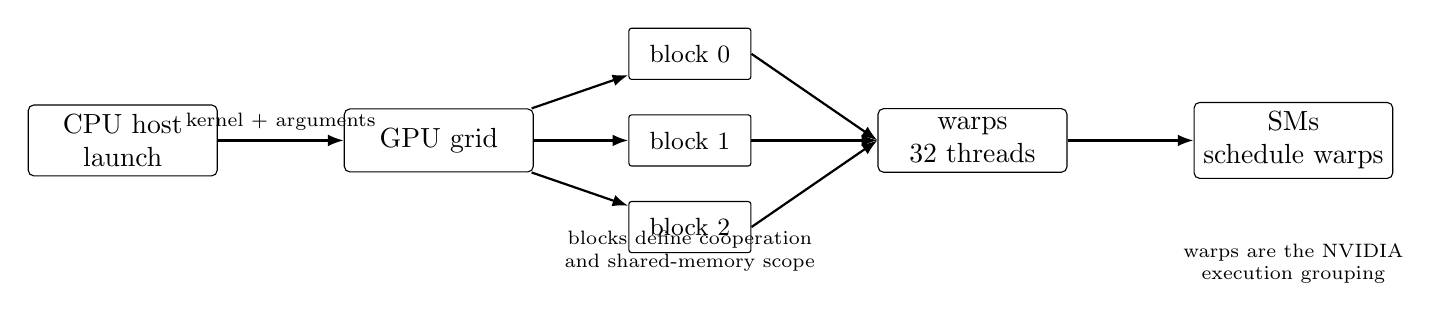
\begin{tikzpicture}[
      arr/.style={-{Latex[length=2mm]}, thick},
      box/.style={draw, rounded corners=2pt, minimum width=2.4cm, minimum height=8mm, align=center},
      smallbox/.style={draw, rounded corners=1pt, minimum width=1.55cm, minimum height=6.5mm, align=center, font=\small}
    ]
    \node[box] (host) {CPU host\\launch};
    \node[box, right=16mm of host] (grid) {GPU grid};
    \node[smallbox, right=12mm of grid, yshift=11mm] (b0) {block 0};
    \node[smallbox, right=12mm of grid] (b1) {block 1};
    \node[smallbox, right=12mm of grid, yshift=-11mm] (b2) {block 2};
    \node[box, right=16mm of b1] (warps) {warps\\32 threads};
    \node[box, right=16mm of warps] (sms) {SMs\\schedule warps};
    \draw[arr] (host) -- node[above,font=\scriptsize]{kernel + arguments} (grid);
    \draw[arr] (grid) -- (b0);
    \draw[arr] (grid) -- (b1);
    \draw[arr] (grid) -- (b2);
    \draw[arr] (b0.east) -- (warps.west);
    \draw[arr] (b1.east) -- (warps.west);
    \draw[arr] (b2.east) -- (warps.west);
    \draw[arr] (warps) -- (sms);
    \node[font=\scriptsize, align=center, below=7mm of b1] {blocks define cooperation\\and shared-memory scope};
    \node[font=\scriptsize, align=center, below=7mm of sms] {warps are the NVIDIA\\execution grouping};
    \end{tikzpicture}%
    }
    \caption{Software decomposes a kernel into blocks and threads; NVIDIA hardware schedules threads in warps onto streaming multiprocessors (SMs).}
    \label{fig:gpu-execution}
\end{figure}

\paragraph{Blocks, Threads, Warps, and SMs}
A \textbf{thread} is the logical execution instance exposed by CUDA, it is the bit of the GPU that does your computation.
It is the soldier.
CUDA groups threads into blocks, and hardware organises each block into warps.
A \textbf{block} groups threads that can share memory and barriers, meaning they might read the same input data and do different computations on it.
These are like regiments or other large management structures which operate on shared plans.
A \textbf{warp} is then a cluster of (normally) 32 threads which are scheduled together by the \textbf{Streaming Multiprocessor} (SM).
The SM is like a planning division of the army and the warp is a small group of synchronised soldiers like a platoon or squad.

If a block contains only 10 threads, it still occupies one 32-lane warp, but only 10 lanes are active.
The other 22 lanes produce no results, just like how squad/platoons are deployed together.

\begin{calloutmemoryhook}
Blocks let threads share memory and synchronise.
SMs schedule their warps.
Warps are groups of 32 threads executing together, like a squad/platoon.
\end{calloutmemoryhook}

\paragraph{Time on Host versus Device.}

The CPU queues work to the GPU, it does not actually call GPU threads.
With asynchronous CPU queue adds, the measured program and the completed device work are not necessarily at the same point in time.
This time discrepancy is a common profiling error.

\paragraph{Memory Hierarchy}
\begin{figure}[H]
\centering
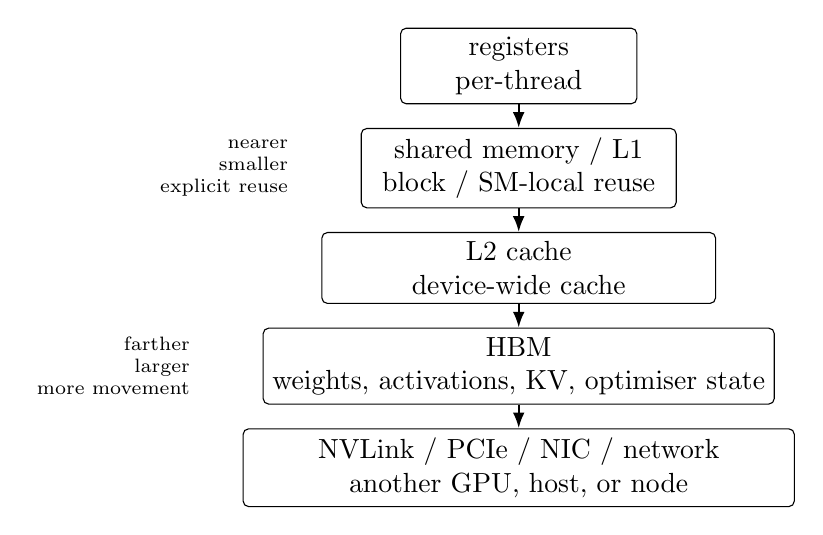
\begin{tikzpicture}[
  level/.style={draw, rounded corners=2pt, align=center, minimum height=7mm},
  arr/.style={-{Latex[length=2mm]}, thick}
]
\node[level, minimum width=3.0cm] (reg) {registers\\per-thread};
\node[level, minimum width=4.0cm, below=3mm of reg] (shared) {shared memory / L1\\block / SM-local reuse};
\node[level, minimum width=5.0cm, below=3mm of shared] (l2) {L2 cache\\device-wide cache};
\node[level, minimum width=6.0cm, below=3mm of l2] (hbm) {HBM\\weights, activations, KV, optimiser state};
\node[level, minimum width=7.0cm, below=3mm of hbm] (links) {NVLink / PCIe / NIC / network\\another GPU, host, or node};
\draw[arr] (reg) -- (shared);
\draw[arr] (shared) -- (l2);
\draw[arr] (l2) -- (hbm);
\draw[arr] (hbm) -- (links);
\node[font=\scriptsize, align=right, left=8mm of shared] {nearer\\smaller\\explicit reuse};
\node[font=\scriptsize, align=right, left=8mm of hbm] {farther\\larger\\more movement};
\end{tikzpicture}
\caption{Qualitative accelerator memory hierarchy. 
The main concern is which values can be loaded once and reused before they fall to a slower level.}
\label{fig:gpu-memory-hierarchy}
\end{figure}

\paragraph{Registers and Shared memory}
Registers are the fastest, lowest-level on-chip memory unit by providing fast per-thread storage.
More register or shared-memory use can reduce HBM traffic, but both consume SM resources and can reduce the number of resident warps or blocks.
For soldiers, carrying a notepad avoids repeated trips to a depot, but limited space for equipment means fewer soldiers can work at once.


\paragraph{Coalescing}
Memory coalescing is a GPU hardware optimisation technique that combines separate global memory (DRAM) access requests from multiple threads in a warp into a single, consolidated memory transaction.
Neighbouring threads should ideally request memory in a pattern that can be served by a small number of memory transactions.
This means delivering adjacent supplies together in a small number of trips, rather than sending a vehicle per soldier.


\paragraph{Tiling}
A tile loads a chunk into a nearby memory level and reuses it across several operations.
GEMM, convolution, attention, transpose, and many reductions differ in mathematics but reuse the same systems idea: \textit{one expensive load should pay for as much useful work as possible}.
Imagine bringing a batch of supplies into a nearby depot and reusing them across many tasks before fetching the next batch.

\paragraph{Occupancy}
This is the ratio of active concurrent warps on a GPU's SM to the maximum number of active warps.
Resident warps hide latency because the scheduler can switch to independent work, but maximum occupancy is not the objective.
A kernel can be faster at lower occupancy if a larger tile, more registers, or more shared memory increases useful work per byte enough to compensate.
As a general, ask yourself: \textit{How many platoons can remain ready at this worksite, against its capacity?}

\begin{calloutdegreeexperiment}
    For one kernel, useful variables include tile shape, threads or warps, pipeline stages, vector width, dtype, tensor layout, shared-memory use, register pressure, launch grid, and fusion boundary.
\end{calloutdegreeexperiment}

\section{Performance Arithmetic}
\label{sec:hardware-roofline}
The balance between \textit{waiting for data} and \textit{computation is slow} is the \textbf{arithmetic intensity}:
\[
    \underbrace{I}_{\text{arithmetic intensity}}
    =
    \frac{\overbrace{N_{\text{useful FLOPs}}}^{\text{arithmetic}}}
    {\underbrace{N_{\text{bytes crossing the boundary}}}_{\text{movement}}}.
\]
A simple bound is
\[
    \underbrace{P_{\text{achievable}}}_{\text{FLOP/s}}
    \leq
    \min\!\left(
    \underbrace{P_{\text{peak compute}}}_{\text{compute roof}},
    \underbrace{B_{\text{memory}}I}_{\text{bandwidth roof}}
    \right).
\]

Problems:
\begin{itemize}
    \item \textbf{Bandwidth-bound kernel:} Impacted by fusion, reuse, layout, quantisation, or fewer reads. 
    Not impacted by reducing FLOPS.
    Large invasions are communication limited because you must communicate complex, time sensitive information across a range of tasks in sync - better connection is decisive.
    \item \textbf{Compute-bound kernel: } Impacted by tensor-core use, instruction throughput, precision, or tile scheduling. 
    Individually complex tasks like seizing an armoured bunker require each soldier's raw strength is decisive.
\end{itemize}

\subsection{Performance Arithmetic Order-of-Magnitude Thinking}
Order-of-magnitude estimates can reject impossible designs before a cluster is reserved.
For model state,
\[
\underbrace{M_{\text{weights}}}_{\text{parameter memory}}
\approx
\underbrace{N_{\text{parameters}}}_{\text{parameter count}}
\underbrace{N_{\text{bytes/parameter}}}_{\text{stored precision}},
\]
then gradients, optimiser state, activations, temporary workspaces, and replicas are added separately rather than hidden in one multiplier.
For communication,
\[
\underbrace{T_{\text{message}}}_{\text{transfer time}}
\approx
\underbrace{\alpha}_{\text{startup / latency}}
+
\frac{\overbrace{N_{\text{bytes}}}^{\text{payload}}}
{\underbrace{B_{\text{effective}}}_{\text{achieved path bandwidth}}}.
\]
Tiny synchronising messages care strongly about $\alpha$; large transfers are dominated by achieved bandwidth and topology.

\section{Software}
\label{sec:hardware-api-stack}
PyTorch, Triton, CUDA, CuTe, NCCL, and inference engines are not interchangeable APIs.
They expose different control surfaces over the same computation, so the useful question is how low in the stack the bottleneck forces the implementation to go.

\begin{table}[H]
% TODO Reorder rows into depth order.
\centering
\footnotesize
\caption{API layers expose different choices rather than competing at one level.}
\label{tab:hardware-api-ladder}
\begin{tabularx}{\textwidth}{@{}>{\raggedright\arraybackslash}p{2.55cm}>{\raggedright\arraybackslash}p{2.35cm}>{\raggedright\arraybackslash}X>{\raggedright\arraybackslash}X@{}}
\toprule
\textbf{Layer} & \textbf{Examples} & \textbf{What is described} & \textbf{Use when} \\
\midrule
Model / framework & PyTorch, JAX & tensor program and model semantics & model research; standard operators are sufficient \\
Graph compiler & \shortstack[l]{\texttt{torch.compile},\\XLA} & graph capture, rewrites, fusion, lowering & Python/launch overhead or graph-level fusion matters \\
Kernel DSL & Triton, Pallas & tiled program instances and memory movement & a custom kernel is needed without explicit CUDA thread mechanics \\
CUDA C++ & CUDA & threads, blocks, memory, streams, synchronisation & precise NVIDIA control or unsupported patterns matter \\
Layout / templates & CuTe, CUTLASS & tensor layouts, MMA tiles, staged pipelines & high-end tensor-core kernels and reusable GEMM structure \\
Machine level & PTX / SASS & instructions and target execution & compiler backend, instruction-level debugging, extreme specialisation \\
\shortstack[l]{Communication\\runtime} & NCCL, NVSHMEM, MPI, UCX, UCC & collectives or remote-memory operations & tensors span GPUs or nodes \\
Serving engine & vLLM, SGLang, TensorRT-LLM, Dynamo & requests, KV state, batching, placement & end-to-end inference scheduling dominates \\
\bottomrule
\end{tabularx}
\end{table}

\begin{figure}[H]
\centering
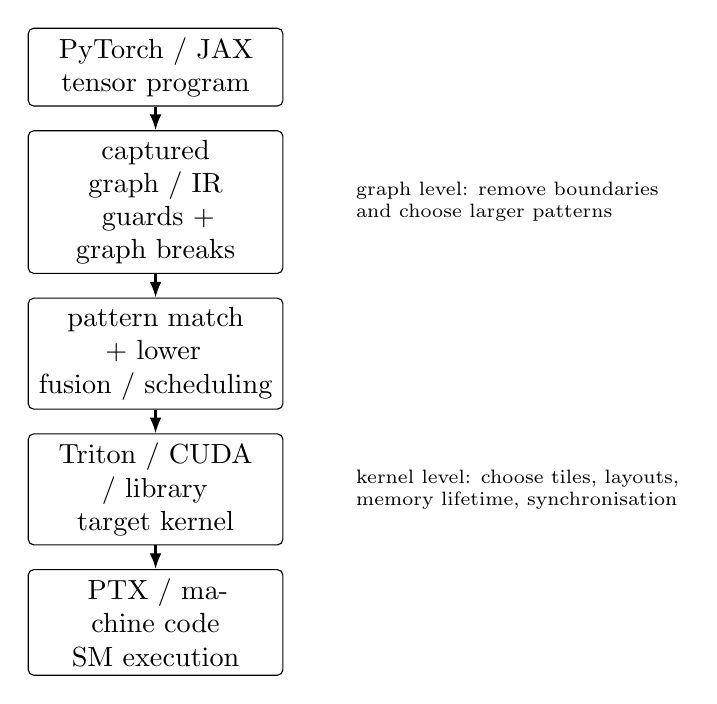
\begin{tikzpicture}[
  box/.style={draw, rounded corners=2pt, minimum height=7mm, text width=3.0cm, align=center},
  arr/.style={-{Latex[length=2mm]}, thick}
]
\node[box] (py) {PyTorch / JAX\\tensor program};
\node[box, below=3mm of py] (graph) {captured graph / IR\\guards + graph breaks};
\node[box, below=3mm of graph] (lower) {pattern match + lower\\fusion / scheduling};
\node[box, below=3mm of lower] (kernel) {Triton / CUDA / library\\target kernel};
\node[box, below=3mm of kernel] (isa) {PTX / machine code\\SM execution};
\draw[arr] (py) -- (graph);
\draw[arr] (graph) -- (lower);
\draw[arr] (lower) -- (kernel);
\draw[arr] (kernel) -- (isa);
\node[font=\scriptsize, align=left, right=8mm of graph] {graph level: remove boundaries\\and choose larger patterns};
\node[font=\scriptsize, align=left, right=8mm of kernel] {kernel level: choose tiles, layouts,\\memory lifetime, synchronisation};
\end{tikzpicture}
\caption{Compilation progressively replaces model-level operations with more explicit scheduling, layout, memory, and target-specific execution choices.}
\label{fig:compiler-lowering}
\end{figure}

\paragraph{CUDA}
CUDA is for NVIDIA execution.
The kernel author (you!) consider thread output ownership, which addresses it loads, whether those loads coalesce, which values are staged in registers or shared memory, which threads synchronise, and which stream carries the work.
A stream is an ordered sequence of GPU work, but remember that independent streams can overlap.
Events can express dependencies without forcing a global host/device synchronisation.

\begin{lstlisting}[language=C++,caption={CUDA exposes thread ownership and launch geometry explicitly.}]
__global__ void relu(float* y, const float* x, int n) {
    int i = blockIdx.x * blockDim.x + threadIdx.x;
    if (i < n) y[i] = max(x[i], 0.0f);
}

relu<<<grid, block, 0, stream>>>(y, x, n);
\end{lstlisting}

\paragraph{Triton}
Triton raises the abstraction boundary by one layer by making the program own vector/tiles and compiling the vector operations onto threads.
This does not remove the hardware constraints, and so poor tile geometry, layout, register pressure, or memory access still produces poor performance.

\begin{lstlisting}[language=Python,caption={Triton exposes program instances, vector offsets, masks, and compile-time tile parameters.},label={lst:triton-kernel}]
@triton.jit
def relu_kernel(x, y, n: tl.constexpr, BLOCK: tl.constexpr):
    pid = tl.program_id(0)
    offsets = pid * BLOCK + tl.arange(0, BLOCK)
    mask = offsets < n
    values = tl.load(x + offsets, mask=mask)
    tl.store(y + offsets, tl.maximum(values, 0.0), mask=mask)
\end{lstlisting}

\paragraph{CuTe and CUTLASS}
CuTe makes tensor layout and thread/value mapping explicit through layout algebra, while CUTLASS provides composable high-performance building blocks for operations such as GEMM.
They become useful when a kernel needs precise tensor-core tiling, staged asynchronous movement, and reusable architecture-specific structure without building the complete machinery from raw CUDA.


\section{Kernels}
\label{sec:hardware-kernels}
A kernel is a GPU program implementing an operation or algorithm; the compiler turns that program into hardware instructions.

You are instructing a soldier not to \textit{capture the bunker with a pincer movement}, you instead tell them \textit{walk 10m to the left, 20m forward, 5m right and fire to the right}. 

\begin{table}[H]
\centering
\small
\caption{Canonical kernels as hardware lessons rather than an algorithm catalogue.
Transpose exposes layout and coalescing; reduction exposes cooperation and synchronisation; GEMM exposes reuse and tensor-core pipelines; attention combines matrix operations, reductions, and a large memory-lifetime problem.}
\label{tab:kernel-patterns}
\begin{tabularx}{\textwidth}{@{}>{\raggedright\arraybackslash}p{2.05cm}>{\raggedright\arraybackslash}X>{\raggedright\arraybackslash}X@{}}
\toprule
\textbf{Kernel} & \textbf{Mechanism to learn} & \textbf{Typical pressure} \\
\midrule
Transpose & remap layout while keeping global accesses coalesced & strided reads or writes; shared-memory bank conflicts \\
Reduction & combine partial values through a tree/hierarchy & synchronisation and falling parallelism late in the reduction \\
Scan & preserve ordered dependencies while parallelising chunks & work efficiency and inter-chunk coordination \\
Online softmax & update stable statistics while streaming a row & extra global passes versus local reduction state \\
GEMM & tile A/B, reuse them, feed tensor-core MMA pipelines & registers/shared memory, layout, pipeline depth, compute throughput \\
Attention & compose tiled GEMM + softmax without full score materialisation & HBM traffic, sequence geometry, reduction state \\
\bottomrule
\end{tabularx}
\end{table}

\paragraph{Fusion.}
Imagine you have two parts of an invasion plan - one for beach landing and another for the inland push.
Sharing a single unified (\textit{fused!}) plan at the start will reduce complexity and communication for the individual soldiers. 
Obviously, this requires larger backpacks to store resources for a longer operation, but it reduces the downtime where the solders (threads) are waiting for instructions - a balance.

\begin{figure}[H]
\centering
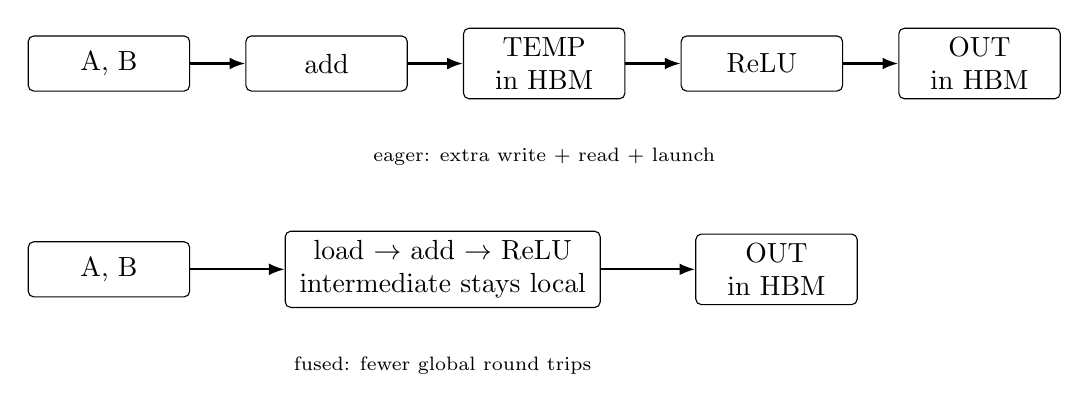
\begin{tikzpicture}[
  box/.style={draw, rounded corners=2pt, minimum width=2.05cm, minimum height=7mm, align=center},
  arr/.style={-{Latex[length=2mm]}, thick},
  note/.style={font=\scriptsize, align=center}
]
\node[box] (a) {A, B};
\node[box, right=7mm of a] (add) {add};
\node[box, right=7mm of add] (tmp) {TEMP\\in HBM};
\node[box, right=7mm of tmp] (relu) {ReLU};
\node[box, right=7mm of relu] (out) {OUT\\in HBM};
\draw[arr] (a) -- (add);
\draw[arr] (add) -- (tmp);
\draw[arr] (tmp) -- (relu);
\draw[arr] (relu) -- (out);
\node[note, below=5mm of tmp] {eager: extra write + read + launch};

\node[box, below=19mm of a] (a2) {A, B};
\node[box, right=12mm of a2, minimum width=4.0cm] (fused) {load $\rightarrow$ add $\rightarrow$ ReLU\\intermediate stays local};
\node[box, right=12mm of fused] (out2) {OUT\\in HBM};
\draw[arr] (a2) -- (fused);
\draw[arr] (fused) -- (out2);
\node[note, below=5mm of fused] {fused: fewer global round trips};
\end{tikzpicture}
\caption{Fusion removes an intermediate memory lifetime and a launch boundary. The trade-off is increased local register/shared-memory pressure and a larger kernel.}
\label{fig:fusion}
\end{figure}

Fusion is not automatically beneficial.
A larger fused kernel can use too many registers, lower occupancy, prevent a tuned library call, or couple operations whose best tile shapes disagree.


\paragraph{GEMM (General Matrix Multiplication) and Tensor Cores}
Matrix multiplication has unusually high reuse potential because one tile of $A$ contributes to many output columns and one tile of $B$ contributes to many output rows.
\[
    \text{HBM tiles}
    &\rightarrow
    \text{shared-memory tiles}
    \rightarrow
    \text{register fragments}
    \rightarrow
    \text{tensor-core MMA}
    \rightarrow
    \text{accumulators}
    \rightarrow
    \text{output tile}.
\]


\paragraph{Low Precision}
Storing large data and models gets expensive and so researchers moved to storing the information in less precise ways, like 16-bit-floating-point, brain-floating-point, to pack more stuff into limited meory space.
FP16/BF16, FP8 families, microscaling formats, and FP4-style formats can reduce bytes per value while enabling higher-throughput tensor-core paths.
The gain appears twice: fewer bytes moved and more arithmetic completed per unit time.
The cost is reduced numerical room plus scale metadata, calibration or dynamic scaling, outlier handling, conversion work, and dependence on a native hardware fast path.


\section{Benchmarking and profiling}
\label{sec:hardware-profiling}
Evaluating your army is vital, and each layer needs evaluating in a different way.
Performance work should move from end-to-end behaviour (general level tactics) to the deepest level (soldier fitness). 

\begin{table}[H]
\centering
\small
\caption{A profiling ladder from model-level behaviour to hardware cause.}
\label{tab:profiling-ladder}
\begin{tabularx}{\textwidth}{@{}>{\raggedright\arraybackslash}p{2.75cm}>{\raggedright\arraybackslash}p{3.0cm}>{\raggedright\arraybackslash}X@{}}
\toprule
\textbf{Tool / level} & \textbf{Question} & \textbf{Typical evidence} \\
\midrule
End-to-end benchmark & Wrong product metric? & step time, tokens/s, p50/p99 latency, scaling efficiency \\
PyTorch profiler & Which operation added cost? & operators, shapes, CPU/GPU activity, memory, communication \\
Nsight Systems & What ran, what waited? & CPU/CUDA timeline, streams, launch gaps, NCCL, copies, overlap \\
Nsight Compute & Why is this hot kernel slow? & memory throughput, cache, occupancy limits, warp stalls, tensor-core use, roofline \\
Fabric microbenchmarks & Is the physical path healthy? & point-to-point/collective latency and achieved bandwidth by topology \\
\bottomrule
\end{tabularx}
\end{table}


\section{Multi-GPU}
\label{sec:hardware-multigpu}
In practice, your army will work as part of a campaign with other armies. 
How do you talk to them efficiently?

Once tensors span accelerators, the physical graph of links becomes part of the algorithm.
External transfers (NVLink/NVSwitch) cost more than internal ones (PCIe, NIC) and so we need to carefully design algorithms to exploit speed in the correct places.

\begin{figure}[H]
\centering
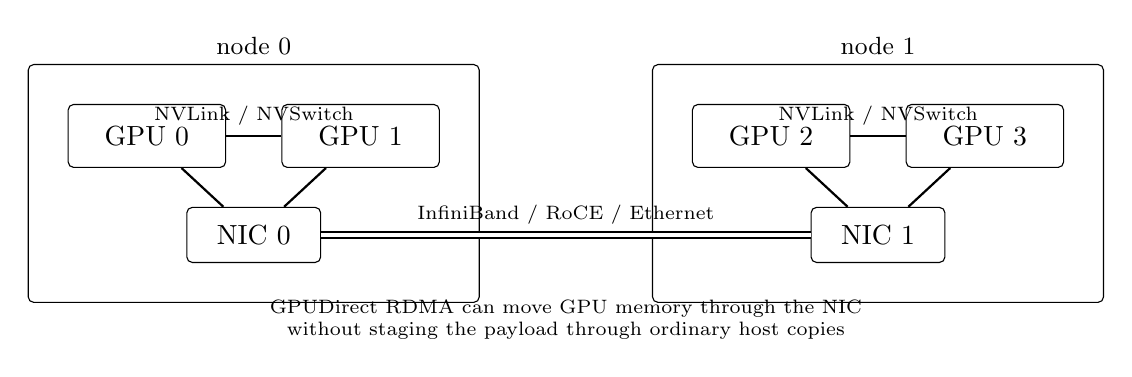
\begin{tikzpicture}[
  gpu/.style={draw, rounded corners=2pt, minimum width=2.0cm, minimum height=8mm, align=center},
  nic/.style={draw, rounded corners=2pt, minimum width=1.7cm, minimum height=7mm, align=center},
  arr/.style={thick},
  net/.style={double, double distance=1.2pt, thick}
]
\node[gpu] (g0) {GPU 0};
\node[gpu, right=7mm of g0] (g1) {GPU 1};
\node[nic, below=9mm of $(g0)!0.5!(g1)$] (n0) {NIC 0};
\draw[arr] (g0) -- node[above,font=\scriptsize]{NVLink / NVSwitch} (g1);
\draw[arr] (g0) -- (n0);
\draw[arr] (g1) -- (n0);
\node[draw, rounded corners=2pt, fit=(g0)(g1)(n0), inner sep=5mm, label={[font=\small]above:node 0}] {};

\node[gpu, right=32mm of g1] (g2) {GPU 2};
\node[gpu, right=7mm of g2] (g3) {GPU 3};
\node[nic, below=9mm of $(g2)!0.5!(g3)$] (n1) {NIC 1};
\draw[arr] (g2) -- node[above,font=\scriptsize]{NVLink / NVSwitch} (g3);
\draw[arr] (g2) -- (n1);
\draw[arr] (g3) -- (n1);
\node[draw, rounded corners=2pt, fit=(g2)(g3)(n1), inner sep=5mm, label={[font=\small]above:node 1}] {};
\draw[net] (n0.east) -- node[above,font=\scriptsize]{InfiniBand / RoCE / Ethernet} (n1.west);
\node[font=\scriptsize, align=center, below=7mm of $(n0)!0.5!(n1)$] {GPUDirect RDMA can move GPU memory through the NIC\\without staging the payload through ordinary host copies};
\end{tikzpicture}
\caption{A logical GPU group sits on heterogeneous links. Rank placement and collective hierarchy should match this topology rather than treating every pair as equivalent.}
\label{fig:multigpu-topology}
\end{figure}


\paragraph{Collectives}
Collectives are communication algorithms we can call atomically.
The main operations and their natural ML uses are compared below.

\begin{table}[H]
\centering
\small
\caption{Collective communication patterns.}
\label{tab:collectives}
\begin{tabularx}{\textwidth}{@{}>{\raggedright\arraybackslash}p{2.25cm}>{\raggedright\arraybackslash}X>{\raggedright\arraybackslash}X@{}}
\toprule
\textbf{Operation} & \textbf{Data movement} & \textbf{Typical ML role} \\
\midrule
Broadcast & one rank sends the same data to the group & initial state / control / parameter distribution \\
Reduce & combine values onto one rank & aggregation when only one consumer needs the result \\
All-reduce & combine, then give the result to every rank & replicated data-parallel gradient synchronisation \\
All-gather & every rank receives every shard & reconstruct sharded activations or parameters \\
Reduce-scatter & reduce, then leave one output shard per rank & sharded gradients/activations; pairs naturally with all-gather \\
All-to-all & each rank sends a different partition to every rank & MoE token dispatch/combine \\
Send / recv & explicit point-to-point exchange & pipeline stage boundaries and specialised transfers \\
\bottomrule
\end{tabularx}
\end{table}

\paragraph{Ring versus Tree}
Rings pass messages in sequence from neighbour to neighbour, while a tree uses hierarchies. 
Rings grow linearly while trees grow log-wise.

\subsection{Communication Interfaces}
\label{sec:hardware-communication-runtimes}
Communication software separates \textbf{what operation is required} from \textbf{which physical transport should carry it}.
This separation is why application code can express an all-reduce while a runtime chooses NVLink, PCIe, InfiniBand, RoCE, or another available path.

\paragraph{Two-Sided versus One-Sided}
Two-sided communication coordinates both endpoints: a send is matched by a receive, or all ranks enter a collective.
One-sided communication lets the initiator name a remote memory operation such as put, get, or atomic without requiring the remote application thread to issue a matching receive at that moment.

\begin{figure}[H]
\centering
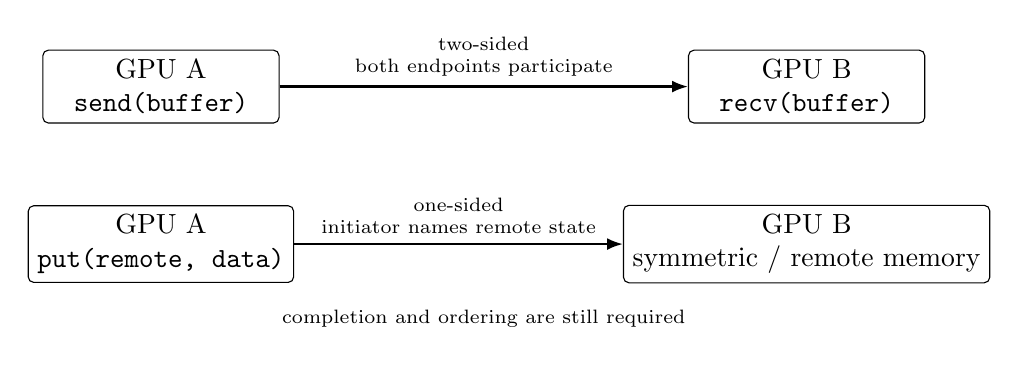
\begin{tikzpicture}[
  box/.style={draw, rounded corners=2pt, minimum width=3.0cm, minimum height=8mm, align=center},
  arr/.style={-{Latex[length=2mm]}, thick}
]
\node[box] (a) at (0,0) {GPU A\\\texttt{send(buffer)}};
\node[box] (b) at (8.2,0) {GPU B\\\texttt{recv(buffer)}};
\draw[arr] (a) -- node[above,font=\scriptsize,align=center]{two-sided\\both endpoints participate} (b);

\node[box] (a2) at (0,-2.0) {GPU A\\\texttt{put(remote, data)}};
\node[box] (b2) at (8.2,-2.0) {GPU B\\symmetric / remote memory};
\draw[arr] (a2) -- node[above,font=\scriptsize,align=center]{one-sided\\initiator names remote state} (b2);
\node[font=\scriptsize, align=center] at (4.1,-2.95) {completion and ordering are still required};
\end{tikzpicture}
\caption{Two-sided communication coordinates operations at both endpoints; one-sided communication exposes remotely addressable state to the initiator.}
\label{fig:one-two-sided}
\end{figure}

\paragraph{Hardware}

\textbf{RDMA} (Remote Direct Access Memory) lets a network adapter transfer registered memory with little ordinary CPU copying or intervention.
GPUDirect RDMA extends this path to GPU memory so a NIC can move data between accelerator memory and the network without staging the payload through CPU memory.


Connections between GPUs exist in two ways.
\begin{itemize}
    \item \textbf{Within a Node:} Communication within the same server (node). 
    This occurs when GPUs installed on the same motherboard or baseboard share data locally, utilising ultra-high-bandwidth interconnects like 
    \begin{itemize}
        \item \textbf{NVLink:} Bi-directional interconnect developed by NVIDIA providing direct GPU-to-GPU communication at speeds significantly faster than traditional PCIe, bypassing the CPU to drastically reduce latency.
        \item \textbf{NVSwitch:} A physical routing chip that extends NVLink connectivity beyond direct point-to-point pairs. 
        It acts as an on-board high-speed switch, allowing all GPUs within a node to communicate simultaneously at NVLink bandwidth, effectively creating a single monolithic virtual GPU pool.
        \item \textbf{PCIe (Peripheral Component Interconnect Express):} The standard system bus interface used to connect GPUs to the CPU and system memory. 
        While it features lower bandwidth and higher latency than NVLink, it serves as the universal hardware baseline across all hardware configurations.
    \end{itemize}
    \item \textbf{Between Nodes:} Communication between different servers (nodes) in a network. 
    This occurs when GPUs housed in separate physical chassis need to share data, typically utilising high-speed networking technologies like:
    \begin{itemize}
        \item \textbf{InfiniBand:} Interconnect with RDMA semantics. Example: \textit{Quantum-X}.
        \item \textbf{RoCE (RDMA over Converged Ethernet):} Use an ethernet connection between nodes using a Network Interface Card (\textbf{NIC}) which is kind of like a driver. 
        Exposes local RDMA to global GPU network. Example: \textit{Spectrum-X}.
    \end{itemize}
\end{itemize}

\paragraph{Software}
We have different layers of software available:
\begin{itemize}
    \item \textbf{NCCL} (pronounced \textit{nickel}) is your high level communication software, it exposes collectives in code as functions (e.g. \textsc{collective(tensor)}) and abstracts away the specific point-to-point communication. 
    In python language, this is what SciPy is to numpy - if you want a common solution, use NCCL.
    \item \textbf{NVSHMEM} is NVIDIA’s parallel programming library that implements an OpenSHMEM-based Partitioned Global Address Space (PGAS) across a cluster of GPUs. 
    In python language, this is what numpy is to SciPy - if you want a custom solution, use NVSHMEM.
    \item \textbf{MPI} is a broad message-passing programming model used throughout HPC.
    \item \textbf{UCX} is a lower communication layer that selects and drives transports, while \textbf{UCC} provides collective operations over underlying communication mechanisms.
\end{itemize}


\section{Distributed Training}
\label{sec:hardware-parallelism}
Some training bottlenecks may be solved by using many GPUs in parallel, for example if datasets can be sharded/partitioned then we may train duplicates of the model independently and synchronise them later - this is \textit{Data Parallel} training.

\begin{table}[H]
\centering
\footnotesize
\caption{Training parallelisms as resource/communication trade-offs.}
\label{tab:parallelisms}
\begin{tabularx}{\textwidth}{@{}>{\raggedright\arraybackslash}p{2.15cm}>{\raggedright\arraybackslash}p{2.15cm}>{\raggedright\arraybackslash}X>{\raggedright\arraybackslash}X@{}}
\toprule
\textbf{Parallelism} & \textbf{Partition} & \textbf{New communication} & \textbf{Use when} \\
\midrule
Data parallel (DP) & data & gradient / parameter-state synchronisation & model fits per worker; more throughput is needed \\
Tensor parallel (TP) & tensor dimensions inside layers & frequent all-reduce, all-gather, reduce-scatter & a layer/model must be split and fast links are available \\
Pipeline parallel (PP) & layer depth (stages) & activations and gradients across stage boundaries & model state must be split by depth \\
Context parallel (CP) & sequence or context dimension & attention and KV exchange & long sequences dominate activation/state memory \\
Expert parallel (EP) & MoE experts & all-to-all token dispatch and combine & sparse expert capacity spans devices \\
ZeRO or FSDP-style & parameters, gradients, optimiser state & state gather/scatter around use/update & replicated training state consumes too much memory \\
\bottomrule
\end{tabularx}
\end{table}


\begin{calloutmemoryhook}
Parallelism turns a resource bottleneck into a communication pattern.
\end{calloutmemoryhook}



\section{Practical Diagnostic Process}
\label{sec:hardware-diagnostic}
We prefer to diagnose from wall-clock symptoms rather than jumping blindly to a solution.


\begin{figure}[H]
\centering
\resizebox{0.98\textwidth}{!}{%
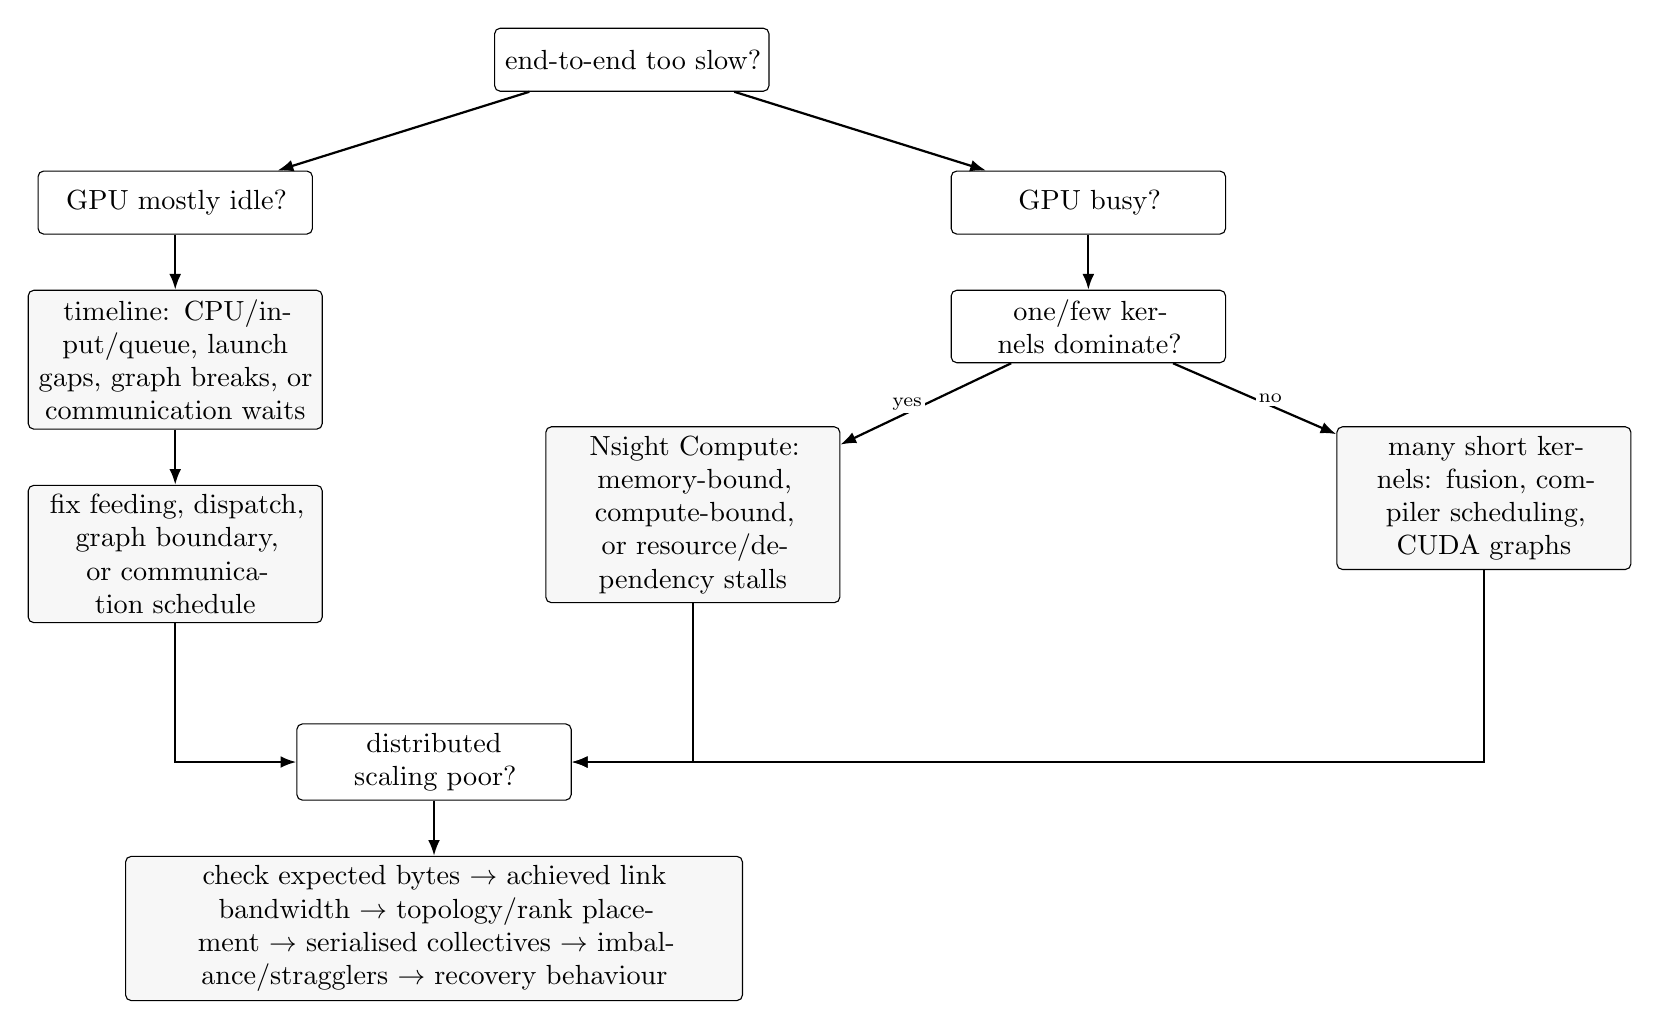
\begin{tikzpicture}[
  node distance=7mm and 8mm,
  q/.style={draw, rounded corners=2pt, text width=3.25cm, align=center, minimum height=8mm},
  a/.style={draw, rounded corners=2pt, text width=3.5cm, align=center, minimum height=8mm, fill=black!3},
  arr/.style={-{Latex[length=2mm]}, thick},
  edge/.style={font=\scriptsize, fill=white, inner sep=1pt}
]
\node[q] (slow) {end-to-end too slow?};
\node[q, below left=10mm and 23mm of slow] (idle) {GPU mostly idle?};
\node[q, below right=10mm and 23mm of slow] (busy) {GPU busy?};
\draw[arr] (slow) -- (idle);
\draw[arr] (slow) -- (busy);

\node[a, below=of idle] (host) {timeline: CPU/input/queue, launch gaps, graph breaks, or communication waits};
\draw[arr] (idle) -- (host);
\node[a, below=of host] (hostfix) {fix feeding, dispatch, graph boundary, or communication schedule};
\draw[arr] (host) -- (hostfix);

\node[q, below=of busy] (hot) {one/few kernels dominate?};
\draw[arr] (busy) -- (hot);
\node[a, below left=8mm and 14mm of hot] (kernel) {Nsight Compute: memory-bound, compute-bound, or resource/dependency stalls};
\node[a, below right=8mm and 14mm of hot] (many) {many short kernels: fusion, compiler scheduling, CUDA graphs};
\draw[arr] (hot) -- node[edge,left]{yes} (kernel);
\draw[arr] (hot) -- node[edge,right]{no} (many);

\node[q, below=24mm of $(hostfix)!0.5!(kernel)$] (scale) {distributed scaling poor?};
\node[a, below=of scale, text width=7.6cm] (dist) {check expected bytes $\rightarrow$ achieved link bandwidth $\rightarrow$ topology/rank placement $\rightarrow$ serialised collectives $\rightarrow$ imbalance/stragglers $\rightarrow$ recovery behaviour};
\draw[arr] (hostfix.south) |- (scale.west);
\draw[arr] (kernel.south) |- (scale.east);
\draw[arr] (many.south) |- (scale.east);
\draw[arr] (scale) -- (dist);
\end{tikzpicture}%
}
\caption{Minimal performance diagnostic. The branch selects the next measurement; it does not prescribe an optimisation before the limiting resource is known.}
\label{fig:hardware-diagnostic}
\end{figure}
\chapter{Foundations: Learning Paradigms}
\label{chap:objectives}

\section{Types of Supervision}
\label{sec:objectives-supervised-unsupervised-self-supervised-and-reinforcement-learning}

\begin{table}[htbp]
    \centering
    \small
    \begin{tabularx}{\linewidth}{@{}L{.18\linewidth}YY@{}}
    \toprule
    Paradigm & Training information & Typical goal \\
    \midrule
    Supervised & Input--target pairs & Classification, regression, forecasting \\
    Unsupervised & Inputs without task labels & Density, clustering, compression \\
    Self-supervised & Targets manufactured from inputs & Representation learning from structure in the data \\
    Semi-supervised & Few labels plus many unlabelled examples & Label-efficient prediction \\
    Reinforcement learning & States, actions and rewards through interaction & Policy maximising expected return \\
    \bottomrule
    \end{tabularx}
    \caption{Learning paradigms mainly differ in where the training signal comes from.}
\end{table}

\section{Supervised Losses: Continuous}
\label{sec:objectives-supervised-losses-for-continuous-targets}
For residuals $e_i=y_i-\hat y_i$ over $N_{\text{examples}}$:

\paragraph{MSE} makes large residuals disproportionately expensive and matches constant-variance Gaussian observation noise up to scale/constants.
\[
    \mathrm{MSE}&=\frac{1}{N_{\text{examples}}}\sum_i e_i^2.
\]
\paragraph{MAE} grows linearly with residual size and matches a Laplace-like noise model.
\[
    \mathrm{MAE}&=\frac{1}{N_{\text{examples}}}\sum_i |e_i|.
\]
\paragraph{RMSE} restores target units and is often more useful for reporting than for changing the optimiser itself. 
See \cref{sec:evaluation-regression-metrics}.
\[
    \mathrm{RMSE}&=\sqrt{\mathrm{MSE}}.
\]
\paragraph{Huber} loss is quadratic near zero and linear for large residuals:
\[
    \ell_{\delta}(e)
    =
    \begin{cases}
    \frac12e^2,&|e|\le\delta,\\
    \delta\left(|e|-\frac12\delta\right),&|e|>\delta.
\end{cases}
\]
It preserves a smooth small-error region while reducing the influence of large outliers relative to MSE.

\begin{calloutmemoryhook}
MSE squares outliers and MAE does not. Huber is quadratic near zero and linear far away.
\end{calloutmemoryhook}

\section{Supervised Losses: Discrete}
\label{sec:objectives-classification-losses-and-logits}
A logit is a number between which we map to a probability, for example we might say that a score out of 100 of 34 is more likley than not a 0 in a binary system.
A binary logit $a$ is $p=\sigma(a)$ and,
\paragraph{Binary Cross-Entropy} is
\[
    \ell_{\mathrm{BCE}}
    =
    -\underbrace{y\log p}_{\text{reward positive probability when }y=1}
    -\underbrace{(1-y)\log(1-p)}_{\text{reward negative probability when }y=0}.
\]
Use implementations that combine the logit and BCE calculation for numerical stability.
Independent sigmoid/BCE outputs suit labels that can be simultaneously true.

For $N_{\text{classes}}$ mutually exclusive classes, softmax converts logits to a probability:
\[
    p_i
    =
    \frac{e^{a_i}}{\sum_{j=1}^{N_{\text{classes}}}e^{a_j}}.
\]
\paragraph{Categorical Cross-Entropy} for the true class is $-\log p_{\text{true class}}$.
Training loss and deployment metric are separate design choices; accuracy, precision/recall and F1 are in \cref{sec:evaluation-classification-evaluation-the-confusion-matrix,sec:evaluation-precision-recall-and-f1}.


\subsection{Differentiating Categories}
\label{sec:models-gumbel-softmax-differentiable-categorical-choices}
A hard categorical sample blocks ordinary pathwise gradients.
Gumbel--Softmax replaces the hard one-hot choice during optimisation with a temperature-controlled softmax of noisy category logits:
\[
    \underbrace{y_i}_{\text{soft category weight}}
    =
    \operatorname{softmax}_i\!\left(
    \frac{\underbrace{\log\pi_i}_{\text{category log-weight}}+\underbrace{g_i}_{\text{Gumbel noise}}}{\underbrace{\tau}_{\text{temperature}}}
    \right).
\]
Lower temperature makes the vector more nearly one-hot but also makes gradients more brittle.
A straight-through variant uses a hard forward choice with an approximate backward gradient.

\section{Supervised Losses: Ranking and Preference}
\label{sec:objectives-ranking-and-preference-objectives}
Ranking differs from ordinary regression because the useful output is an ordering rather than a numerically calibrated score, which exposes many different dimensions we may evaluate.
\begin{center}
    \small
    \begin{tabularx}{.96\linewidth}{@{}L{.18\linewidth}L{.28\linewidth}Y@{}}
    \toprule
    \textbf{Objective} & \textbf{Training question} & \textbf{Main trade-off} \\
    \midrule
    Pointwise & Is this item good? & Simple, but treats ranking as independent prediction \\
    Pairwise & Should item $a$ rank above $b$? & Direct ordering signal; creates many possible pairs \\
    Listwise & Is the whole ordered list useful? & Closest to ranking metrics; optimisation is less direct \\
    \bottomrule
    \end{tabularx}
\end{center}

A pairwise model needs only score differences:
\[
    \underbrace{P(a\succ b)}_{\text{$a$ should rank above $b$}}
    =
    \sigma\!\left(
    \underbrace{s_a-s_b}_{\text{relative score}}
    \right).
\]
This same relative-preference structure reappears in LLM preference optimisation in \cref{sec:llms-preference-optimisation}.

Listwise metrics such as \textbf{NDCG} care much more about mistakes near the top of the ranking.
Sorting is discrete, so small score changes can leave NDCG unchanged until two items swap order.
Therefore, methods such as \textbf{LambdaRank} use smooth pairwise updates whose strength reflects how much a swap would change the ranking metric.
The boosted-tree form \textbf{LambdaMART} is linked in \cref{subsec:trees-lambdamart}.

\section{Supervised Losses: Representation}
\label{sec:objectives-representation-learning-objectives}
\paragraph{Reconstruction} objective asks an encoder/decoder pair to preserve information needed to rebuild the input:
\[
    \mathcal L_{\text{reconstruction}}
    =
    \left\|x-g_{\theta_{\text{decoder}}}(f_{\theta_{\text{encoder}}}(x))\right\|_2^2.
\]
Reconstruction does not guarantee preservation of task-relevant information.

\paragraph{Contrastive} objectives instead shape relative geometry.
A triplet-style objective says ``positive closer than negative by a margin'':
\[
    \mathcal L_{\text{triplet}}
    =
    \max\left(0,
    \underbrace{d(z_{\text{anchor}},z_{\text{positive}})}_{\text{pull together}}
    -
    \underbrace{d(z_{\text{anchor}},z_{\text{negative}})}_{\text{push apart}}
    +
    \underbrace{m_{\text{margin}}}_{\text{required separation}}
    \right).
\]
The important experimental choices are how positives/negatives are constructed, which distance is used, and whether augmentations preserve task signal.

\section{Supervised Losses: Variational/Generative}
\label{sec:objectives-variational-and-generative-objectives}
A VAE balances data fit with a structured latent distribution:
\[
    \underbrace{\mathcal L_{\mathrm{VAE}}}_{\text{negative ELBO}}
    =
    \underbrace{-\E_{q_{\theta_{\text{encoder}}}(z\mid x)}\log p_{\theta_{\text{decoder}}}(x\mid z)}_{\text{reconstruction / likelihood}}
    +
    \underbrace{D_{\mathrm{KL}}\!\left(q_{\theta_{\text{encoder}}}(z\mid x)\|p(z)\right)}_{\text{latent prior compatibility}}.
\]
GANs, diffusion models and normalising flows use different objectives; ``generative model'' does not imply this ELBO.

\section{Self-Supervised losses: Reinforcement-Learning}
\label{sec:objectives-reinforcement-learning-objectives}
A policy aims to maximise expected discounted reward:
\[
    \underbrace{J(\theta)}_{\text{policy objective}}
    =
    \E_{\pi_\theta}
    \left[
    \sum_{t=0}^{N_{\text{horizon}}}
    \underbrace{\gamma^t}_{\text{discount}}
    \underbrace{r_t}_{\text{reward}}
    \right].
\]
The optimisation loss may combine policy-gradient, value-error and entropy terms.
Reward, training loss and evaluation metric therefore need not be identical.
Entropy itself is defined in \cref{sec:foundations-entropy}.

\chapter{Data: Preprocessing}
\label{chap:representation}

\section{Curse of Dimensionality}
\label{sec:representation-the-curse-of-dimensionality}
Input data vector spaces grow in size far more than the actual data space.
For example if one drew a map of the world in 2D there woudl be an extremely expressive dataset.
Adding a height dimension to make a 3D map introduces another infinite dimension.
However, this height dimension is \textit{not} fully explored by the data (buildings are only O(10m) tall, planes fly only O(10km) high, \dots) and so there exists a large empty region in our 3D map that goes off to infinity.
This means that all map elements are somewhat close to each other in the height dimension, which obscures many comparisons, like distance metrics.

A simple grid picture makes the scaling really clear, where $N_{\text{points per axis}}^{N_{\text{features}}}$ samples are needed to fill every grid location.

\figpdf[.78\textwidth]{curse_distance}{For one synthetic sample, nearest and farthest distances become less distinguishable as dimension increases.
This illustrates distance concentration rather than asserting a universal law.}

\section{Standardisation}
\label{sec:representation-scaling-standardisation-and-leakage}
\textbf{Standardisation} is the coordinate-wise transform
\[
    x^{\text{standardised}}_j =
    \frac{
    x_j-\mu_j
    }{
    \sigma_{j}
    }.
\]
It equalises scale but does not remove correlations.
It is also known as the \textit{Z-Score}.
Alternatives include:
min--max scaling:
\[
    x^{\text{minmax}}_j = \frac{x - x_{\text{min}}}{x_{\text{max}} - x_{\text{min}}},
\]
robust median/quantile scaling:
\[
    x^{\text{quintile}}_j = \frac{x - \text{median}(x)}{\text{IQR}(x)},
\]
or a physical unit conversion.


\section{Dimensionality Reduction}
\label{sec:representation-dimensionality-reduction-selection-versus-transformation}
\textbf{Feature selection} keeps original variables; \textbf{feature extraction} creates new coordinates.
Selection usually preserves interpretation; extraction can compress correlated structure more efficiently.
L1 regularisation gives a model-based route to sparse selection in settings where individual parameter weights map meaningfully to input features (\cref{sec:stability-regularisation-l1-and-l2}).

\begin{tabularx}{\linewidth}{@{}L{.20\linewidth}YY@{}}
    \toprule
    Method & What it preserves & Main caution \\
    \midrule
    Filter / wrapper selection & Original variables chosen by a criterion & Selection must occur inside CV \\
    PCA & High-variance linear directions & Variance need not predict labels \\
    Autoencoder & Information useful for reconstruction & Reconstruction need not preserve task signal \\
    t-SNE / UMAP & Local neighbourhood structure for visualisation & Global geometry can be distorted \\
    \bottomrule
\end{tabularx}


\paragraph{Distance In High Dimensions is Useless}
In high dimensions distances can become less discriminative. 
As dimensions increase, the dot product between two vectors converges to one. 
At large dimension count, the distance between any two randomly chosen points becomes nearly identical. 
The ratio of the maximum to minimum distance between points approaches 1, making nearest and farthest neighbors almost equidistant.
Solutons:
\begin{itemize}
    \item \textbf{Manhatten Distance:} use the L1 distance metric,
    \item \textbf{Mahalanobis/Ridge Distance:} handle high-dimensional collinearity and small sample sizes better than standard centroid distances,
    \item \textbf{Pre-Reduce Dimensions:} Apply a reduction in advance of any ownstream operation.
\end{itemize}


\section{PCA}
\label{sec:representation-pca-an-eigenvector-view}
For centred data, Principle Componant Analysis (PCA) diagonalises the covariance matrix and keeps the largest-variance eigen-directions:
\begin{equation}
    \underbrace{\Sigma}_{\text{feature covariance}}
    =
    \underbrace{Q}_{\text{variance directions}}
    \underbrace{\operatorname{diag}(\lambda_1,\ldots,\lambda_{N_{\text{features}}})}_{\text{variance scales}}
    Q^\top
    .
\end{equation}
The eigenstructure reminder is in \cref{subsec:la-eigenvectors-and-eigenvalues}.
Keeping the $N_{\text{components}}$ largest-variance directions gives
\[
    z
    =
    Q_{[:N_{\text{components}}]}^\top
    (x-\mu).
\]
Under squared reconstruction error, this is the optimal linear subspace of that rank for the observed data.
Because PCA ignores labels, low-variance predictive signal can be removed.

\section{Whitening: PCA and ZCA}
\label{sec:representation-whitening-pca-and-zca}
Whitening aims for transformed covariance near the identity.
Using the PCA eigensystem, two common transforms are
\begin{align}
    \underbrace{z_{\mathrm{PCAwhite}}}_{\text{whitened in PCA coordinates}}
    &=
    \underbrace{\operatorname{diag}\!\left((\lambda_i+\epsilon)^{-1/2}\right)}_{\text{equalise variance by direction}}
    Q^\top(x-\mu),\\
    \underbrace{z_{\mathrm{ZCA}}}_{\text{whitened near original orientation}}
    &=
    Q\operatorname{diag}\!\left((\lambda_i+\epsilon)^{-1/2}\right)Q^\top(x-\mu).
\end{align}
The stabiliser $\epsilon$ prevents tiny eigenvalues from exploding noise; exact identity covariance is recovered only in the ideal unstabilised full-rank case.
PCA whitening ends in eigenvector coordinates; ZCA rotates back toward the original coordinate orientation.

\figpdf[.96\textwidth]{pca_zca_whitening}{Synthetic correlated data after centring, PCA whitening and ZCA whitening; both decorrelate/rescale, but their output orientations differ.}

\subsection{Whitening versus Normalisation}
\label{sec:representation-whitening-versus-normalisation}
Whitening targets cross-feature linear correlation as well as scale.
Ordinary standardisation changes each feature independently.
BatchNorm, LayerNorm and RMSNorm also normalise selected statistics rather than generally whitening the representation; see \cref{sec:stability-normalisation-control-the-scale-of-intermediate-representations}.

\section{t-SNE, UMAP and latent visualisation}
\label{sec:representation-t-sne-umap-and-latent-visualisation}
t-SNE and UMAP build low-dimensional views that prioritise neighbourhood relationships rather than globally faithful geometry.
UMAP assumes that local neighbour relations reveal a lower-dimensional structure; t-SNE has a neighbourhood-scale hyperparameter commonly called \textbf{perplexity}.
Use either primarily as an exploratory view, not proof that visual clusters are real physical classes.
Check preprocessing, neighbourhood-scale settings, random seeds and external labels before interpreting a plot.

\begin{tabularx}{\linewidth}{@{}L{.21\linewidth}YY@{}}
    \toprule
    Method & Useful assumption & Failure to test \\
    \midrule
    PCA & High variance contains useful linear structure & Signal lies in low-variance directions \\
    Whitening & Linear correlation/scale are nuisance structure & Small-variance directions are mostly noise \\
    t-SNE / UMAP & Local neighbours reveal meaningful organisation & Global distance/cluster appearance is over-interpreted \\
    Autoencoder & Reconstruction preserves useful information & Rare task-critical signal contributes little to average reconstruction \\
    \bottomrule
\end{tabularx}


\chapter{Data: Representation}

When inputting data into a model, we need to consider the structure of the data.
First we must consider the \textit{modality}:
\begin{itemize}
    \item \textbf{Image:} Tensor of height $\times$ width $\times$ colour.
    \item \textbf{Video:} Tensor of height $\times$ width $\times$ colour $\times$ time.
    \item \textbf{Text:} List of \textsc{string}. 
    \item \textbf{Time Series:} Tensor of value $\times$ time. 
    \item The list goes on.
\end{itemize}
Each of these must be transformed into something a model can act upon.

\section{Embedding}
\label{sec:representation-embeddings-as-operational-geometry}
First up, many complex data inputs (text, time series, images) exist in a space that humans can explore (through our eyes, ears, time) but that models cannot.
Embedding is a method of transforming these into a vector space, such that each datapoint exists somewhere in the vector space.
We use an \textit{encoder} for this transformation.
We choose a number of dimensions for this vector space based on computational cost and downstream usefulness.

In theory, similar starting datapoints should be close together in the embedding space - although this is not always true, due to non-linear encodings.

\begin{figure}[htbp]
    \centering
    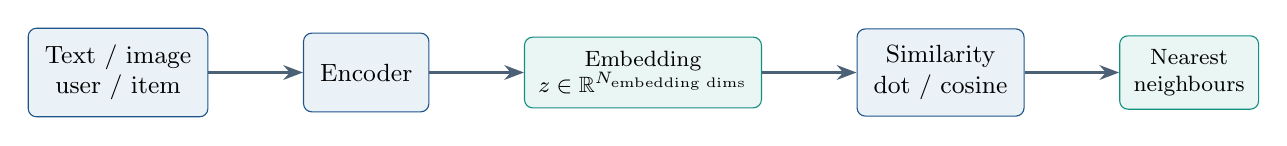
\begin{tikzpicture}[node distance=9mm and 12mm]
    \node[flow] (obj) {Text / image\\user / item};
    \node[flow,right=of obj] (enc) {Encoder};
    \node[yesbox,right=of enc] (vec) {Embedding\\$z\in\R^{N_{\text{embedding dims}}}$};
    \node[flow,right=of vec] (sim) {Similarity\\dot / cosine};
    \node[yesbox,right=of sim] (near) {Nearest\\neighbours};
    \draw[arr] (obj)--(enc);
    \draw[arr] (enc)--(vec);
    \draw[arr] (vec)--(sim);
    \draw[arr] (sim)--(near);
    \end{tikzpicture}
    \caption{A nearest neighbours embedding use-case.}
\end{figure}

\begin{calloutdegreeofexperiment}
Vary encoder objective, embedding dimension, normalisation, similarity function, compression/quantisation and whether one representation must support several retrieval budgets.
\end{calloutdegreeofexperiment}

\paragraph{L2-Normalised Embeddings}
If embeddings are L2-normalised, then the cosine distance metric becomes a simple dot product.
Computing a raw dot product is much faster than computing cosine similarity because it completely skips the square root and division operations required to find vector magnitudes.
Vector databases (like Milvus, Pinecone, or Qdrant) can use hardware-accelerated dot product instructions (MADD / AVX) to search through L2-normalised embeddings at scale, giving you the directional benefits of cosine similarity with the raw speed of a dot product.
A common design question is therefore whether embedding norm should carry task information.


\paragraph{Information Ordered Dimensions}
\textbf{Matryoshka}-style representations ensure that the most important information is packed into the earlier dimensions of a vector, moving part of the quality--cost choice from retraining time to serving time.
\[
    [z_1,\ldots,z_{64}]
    \subset
    [z_1,\ldots,z_{128}]
    \subset
    [z_1,\ldots,z_{N_{\text{embedding dims}}}].
\]
Conceptually, this is \textit{kind of} like making succesive vector spaces out of residuals - however this is not what actually happens.

\paragraph{Quantisation}
Quantising vector element values to fewer bits offers large memory savings.
It is safe to do when the distance metric results remains identical.
This connects directly to model quantisation in \cref{sec:inference-quantisation} and vector search in \cref{sec:llms-rag,sec:ranking-retrieval}.

\section{Tokenisers}
Some data structures, like text and some time-series, are sequences of categories in a very high dimensional space.
For example, there are \textit{about} 26 thousand words in English, and a sentence can be thought of as a path between these words. 
To represent these to models we order the categories and assign them an integer ID number per category.
Those IDs index an embedding matrix:
\[
    E_{\text{token embedding}}
    \in
    \mathbb{R}^{N_{\text{vocabulary}}\times N_{\text{representation dims}}}.
\]
If token ID $791$ occurs, row $791$ is retrieved and its embedding vector available.
The tokeniser itself is normally trained before the language model, so the model inherits those boundaries rather than learning them jointly with its representations.
So the full pipeline is:
\begin{figure}[htbp]
    \centering
    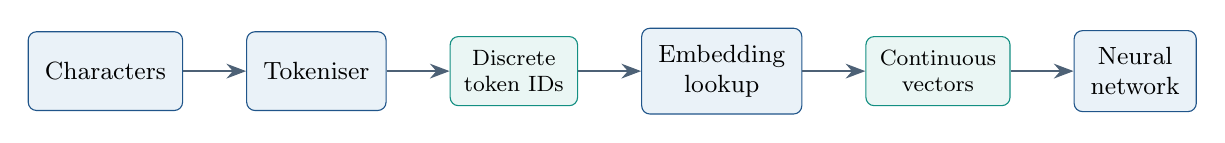
\begin{tikzpicture}[node distance=8mm and 8mm]
    \node[flow] (chars) {Characters};
    \node[flow,right=of chars] (tok) {Tokeniser};
    \node[yesbox,right=of tok] (ids) {Discrete\\token IDs};
    \node[flow,right=of ids] (emb) {Embedding\\lookup};
    \node[yesbox,right=of emb] (vec) {Continuous\\vectors};
    \node[flow,right=of vec] (net) {Neural\\network};
    \draw[arr] (chars)--(tok);
    \draw[arr] (tok)--(ids);
    \draw[arr] (ids)--(emb);
    \draw[arr] (emb)--(vec);
    \draw[arr] (vec)--(net);
    \end{tikzpicture}
    \label{fig:modern-tokenisation-flow}
\end{figure}
For example:
\begin{align}
    &\texttt{``The unbelievable result''}
    \rightarrow
    [\texttt{The},\ \texttt{ unbeliev},\ \texttt{able},\ \texttt{ result}]
    \rightarrow
    \\
    &\rightarrow
    [791,42291,481,1121]
    \rightarrow
    [\mathbf{e}_{791},\mathbf{e}_{42291},\mathbf{e}_{481},\mathbf{e}_{1121}]
    \rightarrow
    \begin{gathered}
    \begin{bmatrix}
        0.12 & -0.43 & 0.87 & 0.21\\
        -0.56 & 0.31 & 0.14 & -0.72\\
        0.93 & -0.18 & 0.45 & 0.06\\
        -0.24 & 0.67 & -0.39 & 0.81
    \end{bmatrix}\\[-1pt]
    \begin{array}{cccc}
        \underbrace{\hphantom{0.12}}_{\mathbf{e}_{791}} &
        \underbrace{\hphantom{-0.43}}_{\mathbf{e}_{42291}} &
        \underbrace{\hphantom{0.87}}_{\mathbf{e}_{481}} &
        \underbrace{\hphantom{0.21}}_{\mathbf{e}_{1121}}
    \end{array}
    \end{gathered}
\end{align}

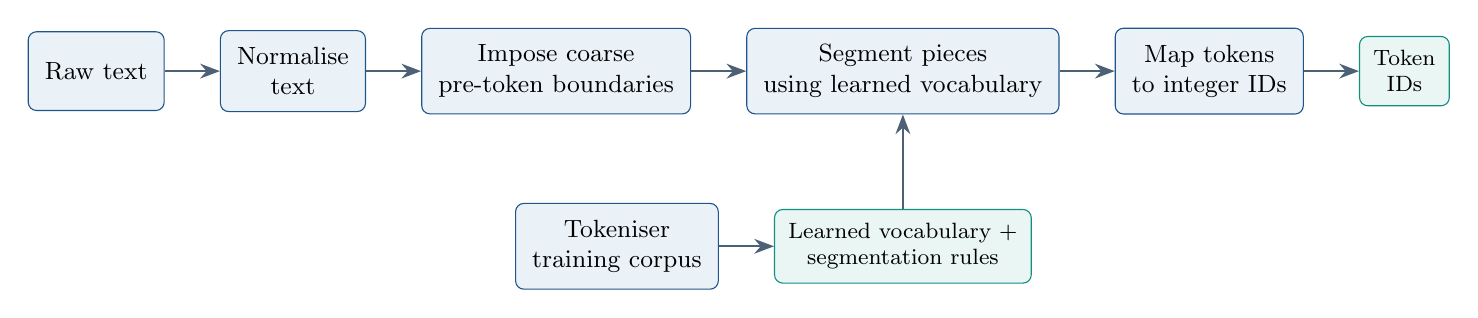
\begin{tikzpicture}[node distance=7mm and 7mm]
    % Tokenisation pipeline
    \node[flow] (raw) {Raw text};
    \node[flow,right=of raw] (norm) {Normalise\\text};
    \node[flow,right=of norm] (pre) {Impose coarse\\pre-token boundaries};
    \node[flow,right=of pre] (seg) {Segment pieces\\using learned vocabulary};
    \node[flow,right=of seg] (map) {Map tokens\\to integer IDs};
    \node[yesbox,right=of map] (ids) {Token\\IDs};
    
    \draw[arr] (raw) -- (norm);
    \draw[arr] (norm) -- (pre);
    \draw[arr] (pre) -- (seg);
    \draw[arr] (seg) -- (map);
    \draw[arr] (map) -- (ids);
    
    % Tokeniser training
    \node[yesbox,below=12mm of seg] (vocab)
        {Learned vocabulary +\\segmentation rules};
    \node[flow,left=of vocab] (train)
        {Tokeniser\\training corpus};
    
    \draw[arr] (train) -- (vocab);
    \draw[arr] (vocab) -- (seg);
\end{tikzpicture}

\paragraph{Level Of Tokeniser}
There are many ways to skin a word, each with different biases. 
For example:
\begin{itemize}
    \item \textit{Why not use words?}
    Because it is not the most efficient decomposition of meaning. 
    It woudl complicate pre/suf-fixes, plurals and other semantic means we use grammar to encode. 
    \item  \textit{Why not use letters?}
    Because the number of possible permutations is enormous.
\end{itemize}

Imagine the token count differences between:
\begin{align}
    & \texttt{[transformational]} \rightarrow \texttt{[transform, ational]} \\
    & \texttt{[transformational]} \rightarrow \texttt{[trans, form, ation, al]} \\
    & \texttt{[transformational]} \rightarrow \texttt{[t, r, a, n, s, f, o, r, m, a, t, i, n, o, a, l]}
\end{align}

The trade-off is vocabulary capacity against sequence length:
\[
    \underbrace{N_{\text{vocabulary}}N_{\text{representation dims}}}_{\text{token embedding parameters}}
    \quad\leftrightarrow\quad
    \underbrace{N_{\text{tokens}}}_{\text{sequence length}}
    \quad\Rightarrow\quad
    \underbrace{N_{\text{tokens}}^2}_{\text{dense attention interactions}}.
\]
A larger vocabulary can compress common strings into fewer model steps (remember that transformers need to \textit{do an inference pass} for each token in a sequence), but spends more parameters on the discrete interface and creates more specialised units.
Smaller units improve coverage and sharing, but lengthen the sequence and consume more context and attention work.

\begin{calloutdegreeofexperiment}
Vary vocabulary size, BPE versus Unigram-style segmentation, byte fallback, multilingual vocabulary allocation, text normalisation and special-token design.
\end{calloutdegreeofexperiment}


\paragraph{Byte-Pair Encoding}
Byte-Pair Encoding (BPE) starts from small units and repeatedly merges the most frequent adjacent pair in the tokenizer-training corpus.
Heuristically,
\[
    [\texttt{l},\texttt{o},\texttt{w}]
    \rightarrow
    [\texttt{lo},\texttt{w}]
    \rightarrow
    [\texttt{low}].
\]
The learned merge ordering is then used to segment new text.
The key assumption is that frequently co-occuring characters should be represented as one object.
This produces useful compression, but frequent strings need not align with human linguistic units.

\paragraph{Unigram}
Unigram removes pieces instead. 
It starts with a large candidate vocabulary, fits a probabilistic segmentation model, then repeatedly removes pieces whose deletion damages the model least.
The useful differentiator is therefore:
\[
    \underbrace{\text{BPE}}_{\text{start small and merge}}
    \qquad\text{vs}\qquad
    \underbrace{\text{Unigram}}_{\text{start large and prune}}.
\]
\paragraph{SentencePiece} SentencePiece is tooling that can implement Unigram or BPE-style tokenisation.

\paragraph{WordPiece} WordPiece is another subword family, as used in BERT, but the heuristic is also the vocabulary-learning objective and the search procedure are design choices rather than immutable parts of ``tokenisation''.
It solves out of vocabulary issues by decomposing unknown words to continuation tokens.


\paragraph{Computational Cost}
Multilingual tokenisers learn a finite vocabulary from a mixture of languages, so high-resource text can receive more reusable pieces while underrepresented languages are split more finely.
The same effect appears for code, mathematical notation, unusual Unicode and numbers: inefficient segmentation means more model steps for the same underlying content.

\paragraph{Byte Fallback}
Byte fallback avoids a hard unknown-token failure by representing unsupported text through bytes, but can make rare strings much longer.

\begin{calloutpractical}
Do not compare per-token perplexity across different tokenisers as though a token were a fixed unit, because the prediction unit itself changed.
\end{calloutpractical}


\subsection{Tokens To Know}

Tokenisers use several conventions to represent subwords, word boundaries, unknown inputs, structural delimiters, and model-specific control information. 
Some are visible markers used when displaying a tokeniser's vocabulary. 
Exact token spellings and availability depend on the model and tokeniser version.
Be aware of these.

\subsubsection{The Classics}

\begin{itemize}
    \item \tok{[UNK]}: Unknown token used when an input cannot be represented by the vocabulary. Common in BERT/WordPiece.
    \item \tok{##}: WordPiece continuation prefix, used by BERT. For example, [\tok{play}, \tok{##ing}] represents ``playing''. The prefix indicates that a piece continues an existing word; it is not a standalone special token.
    \item \tok{</w>}: End-of-word marker used in early BPE implementations, including the original subword-nmt convention. For example, [\tok{low}, \tok{est</w>}].
    \item \tok{@@}: Continuation marker in subword-nmt BPE output. For example, [\tok{play@@}, \tok{ing}] represents ``playing''.
    \item \gspace{} (GPT-2/RoBERTa): Represents the leading-space marker normally displayed as Unicode U+0120. For example, [\tok{Hello}] and [\gspace{}\tok{Hello}] are distinct token representations. The label \gspace{} is a substitute, not the actual vocabulary spelling.
    \item \spmspace{} (SentencePiece): Represents the whitespace marker normally displayed as Unicode U+2581. Used by T5, ALBERT, and several Llama tokenisers. For example, [\spmspace{}\tok{Hello}, \spmspace{}\tok{world}].
    \item \tok{<unk>}: Unknown token in SentencePiece-based vocabularies, including T5 and several older Llama tokenisers.
    \item \tok{<s>}: Beginning-of-sequence token in several model families, including RoBERTa and Llama 2.
    \item \tok{</s>}: End-of-sequence token used by RoBERTa, T5, and Llama 2.
    \item \tok{<pad>}: Padding token used to equalise sequence lengths within a batch.
\end{itemize}

\subsubsection{BERT and WordPiece}

\begin{itemize}
    \item \tok{[CLS]}: Classification token placed at the beginning of a BERT input sequence. For example, [\tok{[CLS]}, \tok{hello}, \tok{world}, \tok{[SEP]}].
    \item \tok{[SEP]}: Separator between segments or sentences, and a sequence terminator in BERT.
    \item \tok{[MASK]}: Mask token used in masked-language-model pretraining, notably BERT. For example, [\tok{The}, \tok{[MASK]}, \tok{runs}].
    \item \tok{[PAD]}: Padding token used in BERT.
    \item \tok{[unused0]}, \tok{[unused1]}, \ldots: Reserved vocabulary entries found in original BERT vocabularies.
    \item \tok{[UNK]}: Unknown token used by BERT's WordPiece tokeniser.
\end{itemize}

\subsubsection{GPT and OpenAI Tokenisers}

\begin{itemize}
    \item \tok{<|endoftext|>}: Document or sequence boundary token used in GPT-2 and later OpenAI tokeniser families.
    \item \tok{<|fim_prefix|>}: Beginning of the prefix region in fill-in-the-middle (FIM) formatting, used by models and tokenisers supporting this convention.
    \item \tok{<|fim_middle|>}: Marker introducing the region to be generated in fill-in-the-middle formatting.
    \item \tok{<|fim_suffix|>}: Introduces the suffix region in FIM formatting. The same spelling also serves as an assistant-turn ending marker in OpenAI's Harmony format, depending on context.
    \item \tok{<|endofprompt|>}: Prompt-ending marker present in some OpenAI tokeniser vocabularies.
    \item \tok{<|disc_score|>}: Auxiliary scoring token present in some OpenAI model formats; not normally part of ordinary user-facing text.
\end{itemize}

\subsubsection{OpenAI Harmony Chat Control Tokens}

\begin{itemize}
    \item \tok{<|im_start|>}: Begins a message, followed by a role such as \tok{system}, \tok{developer}, \tok{user}, \tok{assistant}, or a tool name.
    \item \tok{<|im_sep|>}: Separates a message header from its body.
    \item \tok{<|im_end|>}: Ends a message without necessarily indicating the end of the assistant's turn.
    \item \tok{<|fim_suffix|>}: Marks the end of an assistant turn in Harmony.
    \item \tok{<|ghissue|>}: Handoff marker indicating that the assistant is yielding control, typically to a tool.
    \item \tok{<|meta_sep|>}: Introduces channel metadata, such as \tok{analysis}, \tok{final}, or \tok{commentary}. The channel names are ordinary text rather than special tokens.
    \item \tok{<|meta_start|>}: Introduces constrained-format metadata, such as a JSON output-format designation.
    \item \tok{<|ghreview|>}: Refusal-related marker in certain OpenAI formats.
    \item \tok{<|untrusted_region_start|>} and \tok{<|untrusted_region_end|>}: Mark the beginning and end of untrusted text regions in certain formats.
\end{itemize}

\subsubsection{Llama 2 and Llama 3}

\begin{itemize}
    \item \tok{[INST]}: Begins an instruction block in Llama 2 Chat.
    \item \tok{[/INST]}: Ends an instruction block in Llama 2 Chat.
    \item \tok{<<SYS>>}: Begins the system-prompt region in Llama 2 Chat formatting.
    \item \tok{<</SYS>>}: Ends the system-prompt region in Llama 2 Chat formatting.
    \item \tok{<|begin_of_text|>}: Beginning-of-text token in Llama 3.
    \item \tok{<|end_of_text|>}: End-of-text token in Llama 3.
    \item \tok{<|start_header_id|>}: Begins a message header in Llama 3.
    \item \tok{<|end_header_id|>}: Ends a message header in Llama 3.
    \item \tok{<|eot_id|>}: Ends a message without necessarily ending the assistant's turn in Llama 3.
    \item \tok{<|eom_id|>}: Not a standard Llama 3 message delimiter; included only to distinguish it from actual Llama 3 endings.
    \item \tok{<|finetune_right_pad_id|>}: Padding-related token present in Llama 3 token vocabularies.
    \item \tok{<|start_header_id|>assistant<|end_header_id|>}: Example of a Llama 3 assistant header. The role name \tok{assistant} is ordinary text between special tokens.
    \item \tok{<|start_header_id|>user<|end_header_id|>}: Example of a Llama 3 user header.
    \item \tok{<|start_header_id|>assistant<|meta_sep|>final<|end_header_id|>}: Example of a Llama 3 header containing channel metadata.
    \item \tok{<|start_header_id|>assistant<|meta_sep|>analysis<|end_header_id|>}: Example of a channel-labelled header in formats that use this convention.
\end{itemize}

\subsubsection{T5 and Span Corruption}

\begin{itemize}
    \item \tok{<extra_id_0>}: Sentinel token marking a masked span in T5.
    \item \tok{<extra_id_1>}: Sentinel token marking another masked span.
    \item \tok{<extra_id_2>}, \ldots: Additional span sentinels used during T5-style denoising pretraining.
    \item \tok{</s>}: End-of-sequence token in T5.
    \item \tok{<pad>}: Padding token in T5.
    \item \tok{<unk>}: Unknown token in T5's SentencePiece vocabulary.
\end{itemize}

\subsubsection{Qwen and ChatML-Compatible Models}

\begin{itemize}
    \item \tok{<|im_start|>}: Begins a message in Qwen chat templates.
    \item \tok{<|im_end|>}: Ends a message in Qwen chat templates.
    \item \tok{<|endoftext|>}: End-of-text marker in Qwen vocabularies.
    \item \tok{<|vision_start|>}: Begins visual content in Qwen2-VL.
    \item \tok{<|vision_end|>}: Ends visual content in Qwen2-VL.
    \item \tok{<|image_pad|>}: Image placeholder token in Qwen2-VL.
    \item \tok{<|video_pad|>}: Video placeholder token in Qwen2-VL.
    \item \tok{<|object_ref_start|>}: Object-reference marker in some Qwen multimodal formats.
    \item \tok{<|box|>}: Bounding-box marker in some Qwen vision-language formats.
    \item \tok{<|quad|>}: Quadrilateral geometry marker in some Qwen multimodal formats.
\end{itemize}

\subsubsection{Gemma}

\begin{itemize}
    \item \tok{<bos>}: Beginning-of-sequence token in Gemma.
    \item \tok{<eos>}: End-of-sequence token in Gemma.
    \item \tok{<pad>}: Padding token in Gemma.
    \item \tok{<start_of_turn>}: Begins a conversation turn in instruction-tuned Gemma models.
    \item \tok{<end_of_turn>}: Ends a conversation turn in Gemma.
    \item \tok{<unk>}: Unknown token in Gemma's tokeniser.
\end{itemize}

\subsubsection{Multimodal Tokens}

\begin{itemize}
    \item \tok{<|image|>}: Image marker in some multimodal model formats, including certain OpenAI vision-language formats.
    \item \tok{<image>}: Image placeholder in models such as LLaVA.
    \item \tok{<|audio|>}: Audio-content marker in some OpenAI multimodal formats.
    \item \tok{<|audio_perception|>}: Indicates an incoming-audio perception task in some OpenAI audio formats.
    \item \tok{<|soft_audio_text|>}: Marker associated with incoming audio and text-supervised audio processing.
    \item \tok{<|text_audio|>}: Indicates text associated with generated speech in some OpenAI audio formats.
    \item \tok{<|text_sentinel|>}: Delimits text segments in some speech-related formats.
    \item \tok{<|audio_sentinel|>}: Audio-task boundary marker.
    \item \tok{<|end_of_task|>}: Marks the end of certain audio tasks.
    \item \tok{<|speaker_id_0|>}: Speaker identifier in chunked speech-generation formats.
    \item \tok{<|vector3|>}: Indicates a three-dimensional vector in certain structured multimodal representations.
    \item \tok{<|pose3|>}: Indicates pose-like structured data in certain multimodal vocabularies.
    \item \tok{<|rotation3|>}: Indicates three-dimensional rotation data in certain structured multimodal representations.
\end{itemize}




\subsection{Tokenisation Beyond Text}

Although text begins with space seperated words, images, audio and robot actions are continuous signals.
So, their tokenisers need to learn a continuous representation:
\[
    \underbrace{\text{raw signal}}_{\text{pixels / waveform / actions}}
    \rightarrow
    \underbrace{\text{continuous latent}}_{\text{encoder}}
    \rightarrow
    \underbrace{\text{discrete code}}_{\text{quantiser}}
    \rightarrow
    \underbrace{[i_1,i_2,\ldots,i_{N_{\text{tokens}}}]}_{\text{model sequence}}.
\]
The tokenizer therefore chooses both \textit{what information survives} and \textit{how many model steps are required to carry it}.
Answering two questions (language only cares about the model steps) opens a more expressive research space.

\begin{figure}[htbp]
    \centering
    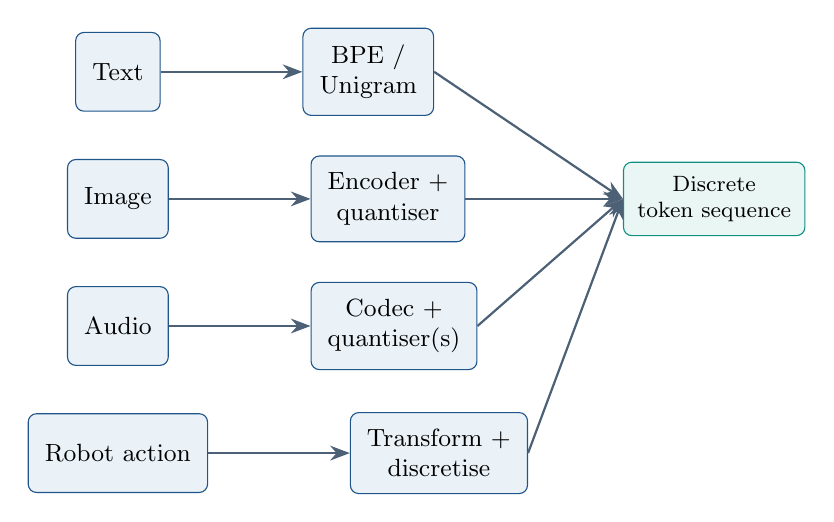
\begin{tikzpicture}[node distance=7mm and 8mm]
    \node[flow] (text) {Text};
    \node[flow,below=6mm of text] (image) {Image};
    \node[flow,below=6mm of image] (audio) {Audio};
    \node[flow,below=6mm of audio] (action) {Robot action};
    
    \node[flow,right=18mm of text] (ttext) {BPE /\\Unigram};
    \node[flow,right=18mm of image] (timage) {Encoder +\\quantiser};
    \node[flow,right=18mm of audio] (taudio) {Codec +\\quantiser(s)};
    \node[flow,right=18mm of action] (taction) {Transform +\\discretise};
    
    \node[yesbox,right=20mm of timage] (tokens) {Discrete\\token sequence};
    \draw[arr] (text)--(ttext);
    \draw[arr] (image)--(timage);
    \draw[arr] (audio)--(taudio);
    \draw[arr] (action)--(taction);
    \draw[arr] (ttext.east)--(tokens.west);
    \draw[arr] (timage.east)--(tokens.west);
    \draw[arr] (taudio.east)--(tokens.west);
    \draw[arr] (taction.east)--(tokens.west);
    \end{tikzpicture}
    \caption{Different physical modalities can be converted into the same sequence abstraction, allowing token-based architectures to operate over more than text.}
    \label{fig:multimodal-tokenisers}
\end{figure}

\paragraph{Images}
VQ-style visual tokenisers encode an image into latent vectors and replace each vector with a discrete code from a learned vocabulary.
The resulting symbols do not need to correspond to literal pixels or fixed image patches.
For example, \textit{TiTok}.

\paragraph{Audio}
Audio tokenisers compress a waveform into discrete symbols at some number of tokens per second.
Residual vector quantisation can apply several codebooks sequentially, with early codes capturing a coarse approximation and later codes encoding what remains.
For example, \textit{SpeechTokenizer} and \textit{MOSS-Audio-Tokenizer}.

\paragraph{Video}
Video adds time to the visual compression problem, so a tokeniser must remove redundancy across space and across neighbouring frames.
\textbf{MAGVIT-v2} is a useful example because one visual vocabulary can encode both images and videos.
\textbf{Emu3} allows text, image and video to all be converted to discrete sequences and trained with one next-token Transformer.

\paragraph{Robot actions}
A robot policy can also turn continuous trajectories into symbols and predict them autoregressively.
\textbf{FAST} first transforms action chunks into frequency space using a discrete cosine transform, then discretises/compresses the coefficients into action tokens.
This works because smooth high-frequency trajectories often contain structure that is expensive to represent with independent per-timestep bins.
The tokeniser is therefore deciding what constitutes one predictable unit of behaviour, not merely how to store a floating-point vector.

\begin{calloutmemoryhook}
A token is a discrete unit over which the model spends sequence compute.
\end{calloutmemoryhook}


\subsection{Research Edge: Fixed Tokens Are Optional}
The standard pipeline makes three strong assumptions that research has attacked.
\begin{itemize}
    \item Fixed vocabulary,
    \item Pre-training boundary decisions,
    \item Tokenisation can be evaluated independently of a model.
\end{itemize}

\begin{table}[htbp]
\centering
\small
\begin{tabular}{p{0.16\textwidth}p{0.25\textwidth}p{0.25\textwidth}p{0.25\textwidth}}
\hline
\textbf{Method} & \textbf{What changes?} & \textbf{Mechanism} & \textbf{New trade-off} \\
\hline
Byte Latent Transformer (BLT) & No fixed subword vocabulary & Raw bytes are grouped into dynamically sized patches; high next-byte entropy creates more boundaries & Tokenisation bias falls, but a learned patching/computation hierarchy replaces it \\
H-Net & Segmentation becomes part of the model & Content- and context-dependent chunks are learned end-to-end from bytes & Removes fixed preprocessing, but makes architecture/training more complex \\
Dynamic tokenisation & Boundaries can change at inference & Frequent subword sequences are merged for the current input and embeddings are predicted on the fly & Shorter sequences without full retraining, but extra machinery and approximation error \\
UniWeTok & Visual vocabulary need not be a small explicit table & A $128$-bit binary visual code implies a code space of size $2^{128}$ & Huge representational space, but code learnability matters as much as nominal capacity \\
ProAct / X-Tokenizer & Reconstruction is not the only action-token objective & Tokens are trained to be predictable, robust or semantically aligned with intended motion & Better policy interface may trade against pure reconstruction fidelity \\
\hline
\end{tabular}
\caption{Research-edge tokenisers mainly change where segmentation lives, how codes are represented, or what objective defines a useful token.}
\label{tab:tokeniser-frontier}
\end{table}

% Research sources used for the appended material:
% Cognetta et al., Tokenization: A Survey for Modern NLP (2026), alphaXiv 2609.tokenization-survey-modern-nlp.
% Pagnoni et al., Byte Latent Transformer: Patches Scale Better Than Tokens, arXiv:2412.09871.
% Hwang, Wang & Gu, Dynamic Chunking for End-to-End Hierarchical Sequence Modeling, arXiv:2507.07955.
% Feher, Vulic & Minixhofer, Retrofitting Large Language Models with Dynamic Tokenization, arXiv:2411.18553.
% Yu et al., An Image is Worth 32 Tokens for Reconstruction and Generation, arXiv:2406.07550.
% Yu et al., Language Model Beats Diffusion -- Tokenizer is Key to Visual Generation, arXiv:2310.05737.
% Wang et al., Emu3: Next-Token Prediction is All You Need, arXiv:2409.18869.
% Zhang et al., SpeechTokenizer: Unified Speech Tokenizer for Speech Large Language Models, arXiv:2308.16692.
% Gong et al., MOSS-Audio-Tokenizer: Scaling Audio Tokenizers for Future Audio Foundation Models, arXiv:2602.10934.
% Pertsch et al., FAST: Efficient Action Tokenization for Vision-Language-Action Models, arXiv:2501.09747.
% Zhuang et al., UniWeTok: An Unified Binary Tokenizer with Codebook Size 2^128, arXiv:2602.14178.
% Chen et al., Beyond Reconstruction: What Matters in Action Tokenization for Robot Policies?, arXiv:2610.09170.
% Kang et al., X-Tokenizer: A Multimodal Action Tokenizer for Vision-Language-Action Pretraining, arXiv:2606.14752.
% Li et al., Studying Image Tokenizers as Visual Languages in Unified Multimodal Models, arXiv:2609.09143.



\section{Position Embeddings}
Sequence modelling contains another representation problem: \textit{How do we represent where a datapoint is in a sequence?}
On one hand, a monotonically increasing (counting up) index would make sense, but in ML world nothing in simple. 
However, an unbounded numerical input is a recipie for disaster to our delicate models and the difference between two indices does not provide the model with a rich representation of positional relationships.
We want a representation that is numerically well-behaved, compatible with the model's embedding dimensions, and capable of encoding useful relationships between positions.
Imagine these two sequences:
\[
    \texttt{dog bites man}
    \qquad\text{and}\qquad
    \texttt{man bites dog}.
\]
RNNs have the order physically encoded though computation.
Self-attention receives a set of vectors but does not know the order, and so need \textbf{position injected explicitly}.

\subsection{Sinusoidal positional encoding}
\label{subsec:modern-sinusoidal-position}
The original Transformer paper added a positional vector to each token embedding.
Each dimension oscillates at a different frequency, creating a bank of clocks.
\[
    PE(\text{position},2i)
    =
    \sin\!\left(
    \frac{\text{position}}{10000^{2i/N_{\text{representation dims}}}}
    \right)
\]
and
\[
    PE(\text{position},2i+1)
    =
    \cos\!\left(
    \frac{\text{position}}{10000^{2i/N_{\text{representation dims}}}}
    \right).
\]

\begin{figure}[htbp]
    \centering
    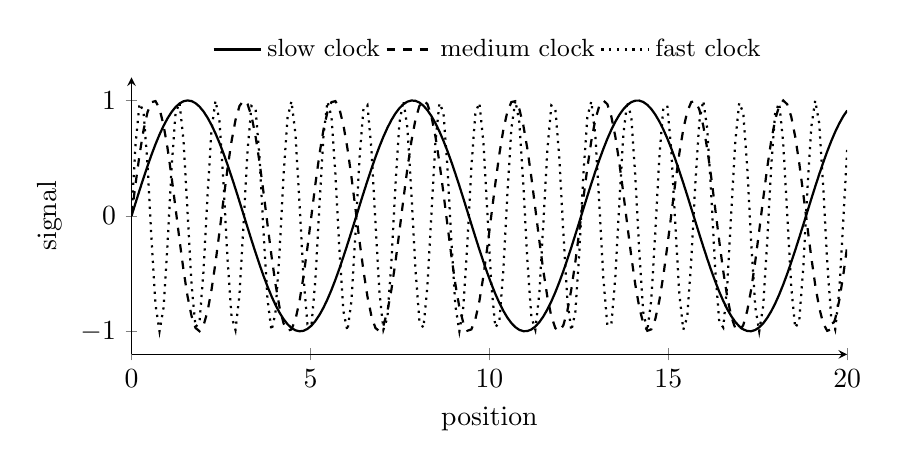
\begin{tikzpicture}
    \begin{axis}[
    width=.88\linewidth,height=5.1cm,
    axis lines=left,
    xlabel={position},
    ylabel={signal},
    xmin=0,xmax=20,ymin=-1.2,ymax=1.2,
    xtick={0,5,10,15,20},ytick={-1,0,1},
    legend style={draw=none,fill=none,font=\small,at={(.5,1.02)},anchor=south,legend columns=3}
    ]
    \addplot[domain=0:20,samples=180,thick] {sin(deg(x))};
    \addlegendentry{slow clock}
    \addplot[domain=0:20,samples=180,thick,dashed] {sin(deg(2.5*x))};
    \addlegendentry{medium clock}
    \addplot[domain=0:20,samples=180,thick,dotted] {sin(deg(6*x))};
    \addlegendentry{fast clock}
    \end{axis}
    \end{tikzpicture}
    \caption{Sinusoidal position uses many frequencies: a position is identified by the joint phase pattern rather than one scalar coordinate.}
    \label{fig:modern-sinusoidal-clocks}
\end{figure}
Position 17 produces one particular pattern across all those clocks.
Position 18 produces another.
Together, the frequencies form a distinctive coordinate system.
For those who are \textit{Physics minded} among you: this is analogous to using multiple Fourier frequencies.

\paragraph{Why the Trig?}
Because
\[
    \sin(a+b)=\sin a\cos b+\cos a\sin b,
\]
information about $\text{position}+k$ can be related algebraically to information about $\text{position}$.



\subsection{Relative Positional Embeddings}
\label{subsec:modern-relative-position}
The sinusoidal model is fundamentally given something resembling ``I am position 734''.
But many language relationships are naturally about ``that token is 3 tokens behind me'', which motivates \textbf{relative position}.
Consider:
\[
    \texttt{The dog that chased the cat was tired.}
\]
For many relationships, the important quantity is not
\[
    \texttt{dog}=\text{position }2,
    \qquad
    \texttt{cat}=\text{position }6,
\]
but something closer to
\[
    \texttt{cat is }+4\texttt{ relative to dog}.
\]

Relative positional methods inject information based on
\[
    \text{key position}-\text{query position}.
\]
Conceptually:
\[
    \underbrace{\text{token A}=500,\quad \text{token B}=503}_{\text{absolute}}
    \qquad\Longrightarrow\qquad
    \underbrace{\text{B is }+3\text{ from A}}_{\text{relative}}.
\]

\subsection{RoPE --- Rotary Positional Embeddings}
\label{subsec:modern-rope}
RoPE is one of the most important positional mechanisms.
Instead of adding a positional vector to the token embedding, RoPE \textit{rotates query and key vectors according to position}.
Take two dimensions of a query:
\[
    \begin{bmatrix}
    q_1\\q_2
    \end{bmatrix}.
\]
At position $m$, rotate them:
\[
    q'_m=R(m\theta)q \quad k'_n=R(n\theta)k,
\]
and calculate their dot product $(q'_m)^\top k'_n $:
\[
    q^\top R(m\theta)^\top R(n\theta)k 
    =
    R(m\theta)^\top R(n\theta)=R((n-m)\theta).
\]
So the interaction naturally depends on $n-m$:
\[
    (q'_m)^\top k'_n
    =
    q^\top R((n-m)\theta)k.
\]

\begin{figure}[htbp]
    \centering
    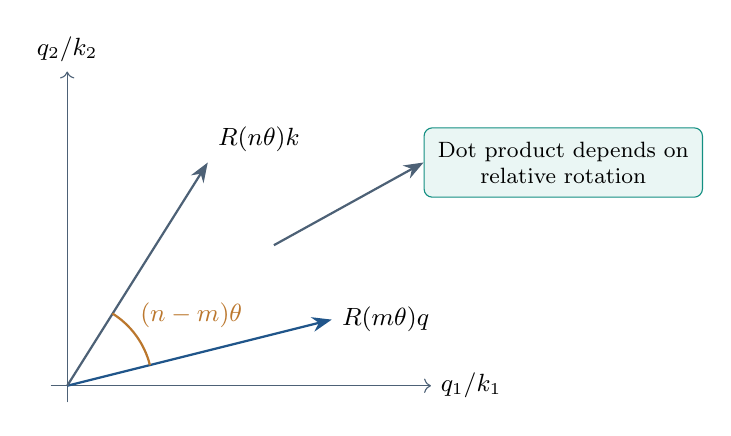
\begin{tikzpicture}[scale=1.05]
    \draw[->,draw=slate] (-.2,0)--(4.4,0) node[right,font=\small] {$q_1/k_1$};
    \draw[->,draw=slate] (0,-.2)--(0,3.8) node[above,font=\small] {$q_2/k_2$};
    \draw[arrblue] (0,0)--(3.2,.8) node[right,font=\small] {$R(m\theta)q$};
    \draw[arr] (0,0)--(1.7,2.7) node[above right,font=\small] {$R(n\theta)k$};
    \draw[draw=amber,thick] (1.0,.25) arc[start angle=14,end angle=58,radius=1.03];
    \node[font=\small,color=amber] at (1.5,.85) {$(n-m)\theta$};
    \node[yesbox] (rel) at (6.0,2.7) {Dot product depends on\\relative rotation};
    \draw[arr] (2.5,1.7)--(rel.west);
    \end{tikzpicture}
    \caption{RoPE turns position into phase: comparing two rotated vectors exposes their relative rotation.}
    \label{fig:modern-rope-geometry}
\end{figure}

\subsubsection*{Why RoPE is Elegant}
It contains both pieces of information:
\[
    \text{position }m\rightarrow\text{rotate }Q\text{ by }m\theta,
    \qquad
    \text{position }n\rightarrow\text{rotate }K\text{ by }n\theta.
\]
So absolute position is used to construct the representation, but \textbf{relative position emerges inside the attention interaction}.
This is a very attractive fit for attention.

\subsubsection*{Sinusoidal vs Relative vs RoPE}
\begin{center}
\small
\begin{tabularx}{.97\linewidth}{@{}L{.18\linewidth}L{.22\linewidth}YY@{}}
\toprule
\textbf{Method} & \textbf{Where position enters} & \textbf{Core idea} & \textbf{Inductive bias} \\
\midrule
Learned absolute & Token representation & Lookup position ID & Every position can learn its own identity \\
Sinusoidal & Token representation & Multiscale periodic coordinates & Smooth structured absolute position \\
Relative & Attention interaction & Explicitly encode displacement & Relationships depend on distance \\
RoPE & Rotate Q/K & Relative information emerges in dot product & Attention similarity should depend naturally on displacement \\
\bottomrule
\end{tabularx}
\end{center}

\begin{calloutmemoryhook}
Sinusoidal: give the token a coordinate.
Relative: tell attention the distance.
RoPE: rotate attention vectors so distance appears geometrically.
\end{calloutmemoryhook}

\subsection{YaRN}
\label{subsec:modern-yarn}
RoPE uses position to rotate queries and keys, but a model trained on a limited context has not learned to interpret arbitrarily large relative rotations.
\textbf{YaRN} (Yet another RoPE extensioN) extends the usable context of an existing RoPE model by changing the rotation frequencies and the scale of attention scores, usually followed by a small amount of long-context fine-tuning.

\paragraph{Interpolate, Rather Than Extrapolate}
A first attempt is \textbf{Position Interpolation}: compress positions so a longer sequence fits inside the original range.
For a model trained on $4\mathrm{k}$ tokens and extended to $64\mathrm{k}$, the position scale is $s=16$, so all RoPE rotations advance $16$ times more slowly.
This extends range but also reduces the angular difference between nearby tokens, weakening local position information.

\paragraph{NTK-by-Parts}
Recall that RoPE uses many rotation frequencies (like the sinusoidal bank of clocks in \cref{subsec:modern-sinusoidal-position}).
High-frequency dimensions rotate many times within the original context and provide fine positional detail; low-frequency dimensions rotate slowly and can help distinguish longer distances.
YaRN therefore \textbf{keeps short-wavelength rotations, stretches long-wavelength rotations, and blends those in-between}:
\[
    \underbrace{s}_{\text{context extension}}
    =\frac{N_{\text{target tokens}}}{N_{\text{trained tokens}}},
    \qquad
    \underbrace{\theta'_i}_{\text{new RoPE frequency}}
    =\underbrace{(1-\gamma_i)\frac{\theta_i}{s}}_{\text{extend long-range phase}}
    +\underbrace{\gamma_i\theta_i}_{\text{preserve local phase}}.
\]
The blending weight $\gamma_i$ runs from $0$ for long wavelengths to $1$ for short wavelengths.
This is called \textbf{NTK-by-parts interpolation}; unlike uniform interpolation, it does not sacrifice every positional frequency to gain context length.

\paragraph{Attention Temperature}
Extending the number of keys can make the attention distribution more diffuse.
YaRN also sharpens the attention logits before the softmax:
\[
    \underbrace{\operatorname{softmax}\!\left(
    \frac{Q_{\text{rotated}}K_{\text{rotated}}^\top}
    {\underbrace{t}_{\text{temperature}}\sqrt{N_{\text{key dims}}}}
    \right)}_{\text{attention over the extended context}},
    \qquad
    \underbrace{\frac{1}{\sqrt{t}}}_{\text{multiply both $Q$ and $K$ by this}}
    \approx 1+0.1\ln(s).
\]
The temperature rule is an empirical fit reported for LLaMA-family models, not a universal constant.
It can be folded into the RoPE query/key scaling, so it need not add a separate attention operation.

YaRN changes \textit{how positions are represented}, not how attention stores or searches history.
Long-context fine-tuning helps the model use the new positional range; it does not remove the extra attention and KV-cache cost of a longer sequence.
The original work extended Llama 2 models towards $64\mathrm{k}$ and $128\mathrm{k}$ contexts with comparatively little additional training.

% Source: Peng et al., YaRN: Efficient Context Window Extension of Large Language Models,
% ICLR 2024; https://arxiv.org/abs/2309.00071.

\chapter{Model Family Overview}
\label{chap:models}

We now will walk though the intuition behind some model families.
Future Chapters dive into some specific model families in a \textit{lot} of detail - these will be skipped here.
Generally, model types in this chapter are outdated, but are kept alive by the \textsc{SciKit-Learn} fans and Coursera\textsuperscript{TM}. 
But first, a word about \textit{why} we need to impose assumptions on our models. 


\section{No Free Lunch}
\label{chap:nfl}

\subsection{Finite Observations Do Not Generalise}
\label{sec:nfl-why-finite-observations-are-not-enough}
The observations $(1,2)$, $(2,4)$ and $(3,6)$ fit both
\[
    f_1(x)=2x,
    \qquad
    f_2(x)=2x+(x-1)(x-2)(x-3),
\]
yet the functions disagree at unseen inputs.
Intravitally, we should choose the simpler, linear function.
However, this is an assumption we are imposing on our model, and we should remember it.
\figpdf[.79\textwidth]{nfl_two_functions}{Two functions can fit the same observations perfectly and disagree elsewhere; prediction requires a preference among compatible hypotheses.}

\subsection{Occam's Zazor}
\label{sec:nfl-occam-s-razor-is-also-a-bias}
``Prefer simple explanations'' is useful only after choosing what simplicity means.
A periodic physical law can be compact in a Fourier representation and awkward in a polynomial one.

\subsection{NFL is Compatible with our Toolbox}
NFL tells us that \textit{to get better task-specific accuracy we need to add assumptions}.
We add assumptions with almost all of our design choices:
\begin{itemize}
    \item \textbf{Architecture:} Data modality and task assumptions.
    \item \textbf{Statistical Guarantees:} sampling process, a restricted hypothesis family, a loss, or a confidence statement.
    A useful intuition:
    \[
        \underbrace{\text{generalisation gap}}_{\text{population error} - \text{training error}}
        \sim
        \sqrt{\frac{\underbrace{\text{model-class complexity}}_{\text{more hypotheses cost more evidence}}+\underbrace{\text{confidence penalty}}_{\text{stronger guarantee costs evidence}}}{N_{\text{examples}}}}.
    \]
    The exact theorem changes with the assumptions and complexity measure.
    The important point is that guarantees are conditional on structure; they do not contradict an assumption-free averaging theorem.
    \item \textbf{Optimisers:} NFL results average search algorithms over broad objective-function families under their own assumptions.
    Practical optimisers exploit gradients, curvature, smoothness and architecture-specific structure, so they are not being compared under an assumption-free real-world distribution.
    The optimiser evolution in \cref{sec:optimisation-how-optimiser-ideas-evolved-a-branching-genealogy} is therefore a sequence of useful structural bets, not a contradiction of NFL.
    \item \textbf{Domain:} Symmetries, topology, conservation laws, known dynamics, simulator structure or measurement constraints.
\end{itemize}



\section{Linear}
\label{sec:models-linear-models-a-transparent-baseline}
\paragraph{Linear regression} predicts with a feature-wise score:
\[
    \hat y=\underbrace{\theta_{\text{weights}}^\top x}_{\text{weighted features}}+\underbrace{\theta_{\text{bias}}}_{\text{offset}}.
\]
``Linear'' refers to the chosen features.
Adding nonlinear engineered features can create nonlinear relationships in raw-input space while the model remains linear in its parameters.
\paragraph{Logistic regression} passes the same score through a sigmoid to model a binary probability.
\[
    \hat y = \frac{1}{1 + e^{-(\theta_{\text{weights}}^\top x + \theta_{\text{bias}})}}
\]



\section{Support Vector Machines and Kernels}
\label{sec:models-support-vector-machines-and-kernels}
Support Vector Machine (SVM) draws a decision line between classes in the feature space.
We aim to maximise the margin between the \textit{Support Vectors}, which are the closest datapoints either side of the line, and the decision line. 
This decision line is a hyperplane in an N-dimensional space, but just imagine it as drawing lines.


\paragraph{Linear vs. Non-linear SVM}
Linear SVM draws a straight decision boundary in the original feature space. Non-linear SVM uses kernels to construct curved decision boundaries, allowing classes that cannot be separated by a straight line to be distinguished.


\paragraph{Hard vs. Soft}
Hard SVM requires decision lines to exactly differentiate between classes, while soft SVM allows for overlap by penalising overlap weakly with a regularisation parameter.
A linear soft-margin SVM trades margin size against hinge-loss violations:
\[
    \min_{\theta_{\text{weights}},\theta_{\text{bias}}}
    \underbrace{\frac12\|\theta_{\text{weights}}\|_2^2}_{\text{prefer a wider margin / smaller weights}}
    +
    \underbrace{C\sum_{i=1}^{N_{\text{examples}}}
    \max\!\left(0,1-y_i(\theta_{\text{weights}}^\top x_i+\theta_{\text{bias}})\right)}_{\text{penalise margin violations}}.
\]
The first term is an L2-style parameter preference, directly linking the SVM objective to \cref{sec:stability-regularisation-l1-and-l2}.
Larger $C$ makes training violations more expensive relative to margin width.

\paragraph{Support Vector Regression (SVR)}
SVR applies the same principle to continuous targets rather than classes.
Instead of separating classes, we fit a function with an $\epsilon$-wide tolerance around it. 
Predictions within this tolerance incur no loss, while errors outside it are penalised.


\paragraph{Kernels}
When data cannot be separated by a flat line (e.g., one group of points forms a circle inside another group), SVM uses kernel functions (such as Polynomial or Radial Basis Function / RBF kernels). 
When temporarily working in a different feature space, the possibility of drawing a differentiating line is higher. 
The \textit{kernel trick} mathematically projects the data into a higher-dimensional space where a linear hyperplane can separate them.

A kernel replaces explicit feature construction with an inner product in a intermediate feature space:
\[
    \underbrace{k(x,x')}_{\text{similarity used by the model}}
    =
    \left\langle
    \underbrace{\phi(x)}_{\text{implicit features}},
    \phi(x')
    \right\rangle.
\]
A linear separator in that feature space can therefore become nonlinear in the original coordinates.
\figpdf[.9\textwidth]{kernel_feature_map}{A nonlinear boundary in raw coordinates can become simple after a feature transformation; kernels can compute some such similarities without explicitly materialising the feature map.}



\section{Neural Networks}
\label{sec:models-neural-networks-and-nonlinear-activations}
You will hear a lot about Neural networks, and their descendants (RNNs, CNNs, etc.) and I will now introduce their smallest componant. 
Their \textit{LEGO bricks}, from which they are all built from.

\subsection{Neuron}
A neuron is the fundamental computational unit of a neural network.
It receives input values, multiplies by a learned weight, adds a bias, and passes the result through an \textit{activation function}.
\[
    \underbrace{h}_{\text{neuron output}}
    =
    \underbrace{\phi}_{\text{activation}}
    \left(
        \underbrace{\sum_{i=1}^{d} \theta_i x_i}_{\text{weighted inputs}}
        +
        \underbrace{\theta_{\text{bias}}}_{\text{offset}}
    \right).
\]
The weights determine how strongly each input influences the output, while the activation function determines how the combined signal is transformed.

\paragraph{Activation Functions}
The activation functions are where Neural Networks derive their non-linearity.
Sigmoid/tanh saturate at large magnitude, ReLU keeps a constant positive-side derivative but can create inactive units, GELU gives a smooth input-dependent gate-like response.
Activation choice interacts with initialisation and gradient scale in \cref{sec:stability-xavier-glorot-and-he-kaiming-initialisation}.
\figpdf[.81\textwidth]{activations}{Common nonlinearities differ mainly in saturation, zeroing behaviour and local derivative scale.}

\begin{itemize}
    \item \textbf{Linear (Identity):} Returns the input unchanged. Common in regression output layers. $f(x)=x$.

    \item \textbf{Binary Step:} Outputs $0$ or $1$ depending on whether the input crosses a threshold. Used in classical perceptrons, but unsuitable for ordinary gradient-based training. $f(x)=\begin{cases}1 & x\geq0\\0 & x<0\end{cases}$.

    \item \textbf{Sigmoid:} Squashes values into $(0,1)$, useful for binary classification probabilities and gating mechanisms. Can suffer from vanishing gradients. $f(x)=\frac{1}{1+e^{-x}}$.

    \item \textbf{Tanh:} Squashes values into $(-1,1)$, providing zero-centred outputs. Historically common in RNNs and LSTMs. $f(x)=\tanh(x)$.

    \item \textbf{ReLU (Rectified Linear Unit):} Sets negative values to zero and leaves positive values unchanged. Computationally cheap and widely used in neural networks, but can produce permanently inactive neurons. $f(x)=\max(0,x)$.

    \item \textbf{Leaky ReLU:} Like ReLU, but allows a small negative slope to reduce the risk of inactive neurons. $f(x)=\max(\alpha x,x)$, where $0<\alpha<1$.

    \item \textbf{PReLU (Parametric ReLU):} Like Leaky ReLU, but learns the negative slope $\alpha$ during training. $f(x)=\max(\alpha x,x)$.

    \item \textbf{ELU (Exponential Linear Unit):} Behaves like ReLU for positive inputs but smoothly saturates towards $-\alpha$ for negative inputs. $f(x)=\begin{cases}x & x>0\\\alpha(e^x-1) & x\leq0\end{cases}$.

    \item \textbf{SELU (Scaled ELU):} A scaled ELU designed to encourage self-normalising behaviour under specific architectural and initialisation conditions. $f(x)=\lambda\begin{cases}x & x>0\\\alpha(e^x-1) & x\leq0\end{cases}$.

    \item \textbf{GELU (Gaussian Error Linear Unit):} Smoothly gates inputs according to their magnitude, rather than applying ReLU's hard threshold. Common in Transformers such as BERT and GPT-2. $f(x)=x\Phi(x)$, where $\Phi$ is the standard normal CDF.

    \item \textbf{SiLU (Sigmoid Linear Unit / Swish):} Smooth activation that multiplies the input by its sigmoid. Used in architectures such as EfficientNet and Llama's SwiGLU feed-forward layers. $f(x)=x\sigma(x)$.

    \item \textbf{Swish:} Generalised SiLU with an adjustable parameter $\beta$ controlling the sigmoid gate. $f(x)=x\sigma(\beta x)$.

    \item \textbf{Mish:} Smooth, non-monotonic activation combining the input with a softplus transformation. $f(x)=x\tanh(\ln(1+e^x))$.

    \item \textbf{Softplus:} Smooth approximation to ReLU that never produces exactly zero for finite inputs. $f(x)=\ln(1+e^x)$.

    \item \textbf{Softsign:} Smoothly compresses values into $(-1,1)$, with slower saturation than tanh. $f(x)=\frac{x}{1+|x|}$.

    \item \textbf{Softmax:} Converts a vector of logits into a probability distribution whose elements sum to $1$. Common in multiclass classification and attention. $f(x)_i=\frac{e^{x_i}}{\sum_j e^{x_j}}$.

    \item \textbf{GLU (Gated Linear Unit):} Multiplies one learned projection by the sigmoid of another, allowing the network to gate information. $f(x)= (W_a x+b_a)\odot\sigma(W_b x+b_b)$.

    \item \textbf{SwiGLU:} Gated activation combining SiLU with another learned projection. Used in modern Transformer feed-forward networks, including Llama. $f(x)=\operatorname{SiLU}(W_a x+b_a)\odot(W_b x+b_b)$.
\end{itemize}


\subsection{Layers}
We combine many neurons into layers and stack them in sequence.
This gives interesting dimensions of variability, because we can:
\begin{itemize}
    \item \textbf{Add Non-Neuron functions} like Pooling, Attention, Dropout, etc.
    \item \textbf{Loop Layers} by passing outputs back as inputs,
    \item \textbf{Ensure Statistical Properties} like normalisation, 
    \item \textbf{Vary Width \& Depth} Vary the number of neurons per layer and the number of layers in the network 
    \item \textbf{Connect Layers Differently} Skip layers, branch into parallel paths, or combine multiple representations.
    \item \textbf{Share Weights} Reuse the same learned parameters across different positions or time steps.
\end{itemize}

This gives a lot of dimensions researchers can explore, and \textit{many} permutations to investigate.
Heuristically, the study of neural networks is either adding to this list through discovery or experimentally trial-and-error-ing a new permutation.

\subsubsection{Common Layer Types}
\begin{itemize}
    \item \textbf{Dense / Fully Connected:} Connects every input feature to every output neuron. Common in Multi-Layer Perceptrons (MLPs) and classification heads.
    \item \textbf{Convolutional:} Applies small, shared filters across local regions of an input. Common in CNNs for images, audio, and other structured signals.
    \item \textbf{Pooling:} Reduces the spatial or sequence dimensions by aggregating values, commonly using maximum or average pooling.
    \item \textbf{Recurrent:} Reuses a state-update operation across sequence steps, allowing previous information to influence later outputs. Used in RNNs, LSTMs, and GRUs.
    \item \textbf{Embedding:} Maps discrete identifiers, such as token IDs, to learned continuous vectors.
    \item \textbf{Attention:} Computes weighted combinations of representations based on their relevance to one another. Central to Transformers.
    \item \textbf{Normalisation:} Rescales or normalises intermediate activations to improve training behaviour. Examples include Batch Normalisation, Layer Normalisation, and RMSNorm.
    \item \textbf{Dropout:} Randomly masks activations during training to reduce overfitting. Typically disabled during inference.
    \item \textbf{Residual / Skip Connection:} Adds an earlier representation to a later one, allowing information and gradients to bypass intermediate transformations.
    \item \textbf{Gated:} Controls information flow using learned multiplicative gates. Common in LSTMs, GRUs, and modern Transformer feed-forward blocks.
    \item \textbf{Upsampling:} Increases the spatial resolution of a representation. Common in image generation, segmentation, and decoder architectures.
    \item \textbf{Output / Projection:} Maps an internal representation into the required output dimension, such as class logits or vocabulary scores.
\end{itemize}

\section{Model assumptions and inductive biases}
\label{sec:models-model-assumptions-and-inductive-biases}
\Cref{sec:nfl-inductive-bias-the-assumptions-that-make-learning-possible} 
\small
\begin{longtable}{@{}L{.22\linewidth}L{.44\linewidth}L{.25\linewidth}@{}}
\caption{Model families, their structural preference, and a representative useful regime.}\label{tab:model_biases}\\
\toprule
Model & Structural preference / assumption & Potential useful setting \\
\midrule
\endfirsthead
\toprule
Model & Structural preference / assumption & Potential useful setting \\
\midrule
\endhead
Linear / logistic regression & Chosen features combine additively in an affine score & Interpretable baseline effects \\
KNN & Nearby observations should have similar targets & Local smooth structure \\
Kernel SVM & A chosen similarity creates a useful separating feature space & Nonlinear boundaries, moderate data \\
Decision tree & Hierarchical thresholds capture useful interactions & Heterogeneous tabular relations \\
Random forest & Averaging decorrelated trees reduces instability & Nonlinear tabular baselines \\
Gradient boosting & Sequential corrections improve a chosen objective & Structured/tabular data \\
PCA & High-variance linear directions are useful & Compression/exploration \\
Gaussian process & Kernel covariance describes function similarity & Small-data regression with uncertainty \\
MLP & Learned nonlinear compositions capture the relation & General vector inputs \\
CNN & Local patterns repeat across positions & Images/gridded signals \\
RNN / GRU / LSTM & Recurrent state summarises useful past context & Sequences/streaming \\
Transformer & Content-dependent token interactions matter & Context-rich sequence/multimodal tasks \\
GNN & Graph connectivity defines relevant neighbours & Molecules/relational systems \\
SSM / Mamba & Long history can be compressed into evolving state & Long or streaming sequences \\
Autoencoder / VAE & Reconstruction preserves useful latent structure & Compression/generative latents \\
GAN / diffusion / flow & Different generative mechanisms match complex data distributions & Sample/density modelling \\
Mixture of experts & Different inputs benefit from specialist subnetworks & Large conditional-capacity systems \\
Siamese / contrastive & Related examples should be close in learned space & Retrieval/few-shot tasks \\
\bottomrule
\end{longtable}
\normalsize

\chapter{Optimisers}
\label{chap:optimisation}
To actually train a model, we get some data and compute the loss based on the current model, as covered so far.
Then, we start an update step by finding the impact on the loss of changing the model parameters.
We do this by differentiating.
Once we have the dependence from the parameters on the loss, we need to decide how to actually update the parameter. 
To Our toolbox for this contains: information from previous steps, parameter scale and local curvature.

\section{Gradient Descent}

\label{sec:optimisation-gradient-descent-following-the-slope-downhill}
For model parameters $\theta\in\R^{N_{\text{parameters}}}$ and training loss $\mathcal L(\theta)$, gradient descent follows the local negative slope:
\begin{calloutmemorise}
\[
    \underbrace{\theta_{t+1}}_{\text{parameters after update}}
    =
    \underbrace{\theta_t}_{\text{current parameters}}
    -
    \underbrace{\eta}_{\text{learning rate}}
    \underbrace{\nabla_\theta\mathcal L(\theta_t)}_{\text{local uphill direction}}.
\]
\end{calloutmemorise}
The negative gradient is the steepest local descent direction for a fixed-length step measured using ordinary Euclidean distance.
The gradient says which way to move locally, but not how far its approximation remains useful.
A small $\eta$ makes slow progress; a large $\eta$ can cross a valley, oscillate, or diverge.

\begin{calloutexample}
    For $\mathcal L(\theta)=(\theta-3)^2$, every update moves relative to the same optimum at $\theta=3$.
    Changing only $\eta$ changes whether the iterates approach $3$ directly, alternate across it, or move away.
\end{calloutexample}

\figpdf[.98\textwidth]{gradient_descent_rates}{Gradient-descent step size on a quadratic loss: identical objective and start, different learning rates, different stability.}

\textbf{Curvature and Conditioning}
A gradient might be very symmetrically flat or sharply curved, where using the same learning rate in both directions causes slow progress in one and unstable steps in the other.
For a positive-definite quadratic loss with \textbf{Hessian} (second derivative, which shows curvature) $\nabla_\theta^2\mathcal L$, a fixed step is stable when
\[
    0<\underbrace{\eta}_{\text{step size}}
    <\frac{2}{\underbrace{\lambda_{\max}(\nabla_\theta^2\mathcal L)}_{\text{sharpest positive curvature}}}.
\]
The ratio $\lambda_{\max}/\lambda_{\min}$ describes how unequal the curvature is across directions: a narrow valley forces the learning rate to respect its steep direction while movement along its flat direction stays slow.
This is why momentum and curvature-aware methods change the trajectory rather than just increasing the learning rate.
The Hessian itself is introduced in \cref{subsec:la-hessian}.

\subsection{Stochastic Gradient}
\label{sec:optimisation-batch-gradient-descent-vs-sgd-vs-mini-batch-sgd}
Generally, we can't fit a whole dataset into memory at once, so we split it into batches. 
\begin{itemize}
    \item \textbf{Full Batch} GD evaluates the gradient over all $N_{\text{examples}}$ examples before updating,
    \item \textbf{SGD} uses one example, and
    \item \textbf{mini-batch SGD} uses a sampled subset $\mathcal B_t$. This one is the only actually useful one.
\end{itemize}

For mini-batch size $N_{\text{batch}}=|\mathcal B_t|$,
\[
    \underbrace{\theta_{t+1}}_{\text{next parameters}}
    =
    \theta_t-\eta
    \underbrace{\frac{1}{N_{\text{batch}}}
    \sum_{i\in\mathcal B_t}\nabla_\theta\ell_i(\theta_t)}_{g_t:\ \text{sampled estimate of the full gradient}}.
\]
Generally, $g_t$ estimates the full-dataset gradient without a systemic bias, however you cannot depend on a given batch reducing the loss.
With approximately independent per-example gradients, the sampling variance falls roughly as $1/N_{\text{batch}}$, so doubling batch size does not double information per update.

\figpdf[.79\textwidth]{sgd_noise}{Full-gradient descent compared with a noisy mini-batch trajectory: batch sampling perturbs the direction without changing the objective being optimised.}

\begin{center}
    \small
    \begin{tabularx}{.96\linewidth}{@{}L{.21\linewidth}YY@{}}
    \toprule
    \textbf{Gradient} & \textbf{Benefit} & \textbf{Cost / consequence} \\
    \midrule
    Full batch & Low sampling noise; reproducible direction & Expensive updates, little stochasticity, often poor accelerator utilisation at scale \\
    One example (strict SGD) & Cheap individual update & Noisy direction; inefficient small matrix operations \\
    Mini-batch & Efficient hardware use with tunable gradient noise & Larger resident batches need more memory; batch and learning rate interact \\
    \bottomrule
    \end{tabularx}
\end{center}

To choose a batch size, balance statistical behaviour (gradient noise) and hardware (throughput and memory).
The fastest configuration per \emph{step} is rarely the fastest to a target validation loss.

\subsection{Backpropagation}
\label{sec:optimisation-backpropagation-how-gradients-are-calculated}
Backpropagation applies reverse-mode differentiation to the forward computation graph.
This is a lot of long words so I define them as...
\begin{itemize}
    \item \textbf{Reverse-Mode Differentiation} finds the differential result from the end of the graph and works its way forward. 
    If you went forward to back, the permutations consume too much compute, however when done back to front, there is one permutation per parameter, and a cheaper operation.
    \item \textbf{Forward computation graph} is the sequence of operations the data passes through. 
    Some know this as a \textbf{Directed Acyclic Graph} (DAG) but just think of it as a flow chart of operations. 
    For example, data may pass through Layer one, then two, then three.
\end{itemize}

it works by propagating loss back through each operation using the chain rule:
\[
    \underbrace{\frac{\partial\mathcal L}{\partial\theta_j}}_{\text{parameter sensitivity}}
    =
    \underbrace{\frac{\partial\mathcal L}{\partial h}}_{\text{downstream sensitivity}}
    \underbrace{\frac{\partial h}{\partial\theta_j}}_{\text{local sensitivity}}.
\]
The Jacobian in \cref{subsec:la-jacobian} is the vector version of this.
Backprop supplies gradients to SGD, Adam, Newton-like methods and other update rules for them to decide \textit{how} to apply this update.

\section{Optimisers}

Most optimisers modify the raw gradient direction in one of three ways: \textbf{use history}, \textbf{rescale step size}, or \textbf{use relationships between directions}.
The first two operate cheaply per parameter, but the third uses richer geometry at higher (pairwise) computational cost.

\subsection{Consider History: Momentum}
\label{sec:optimisation-momentum-remember-previous-gradient-directions}
SGD with momentum keeps an exponentially decaying average of past gradients:
\[
    \underbrace{m_t}_{\text{running direction}}
    =
    \underbrace{\beta m_{t-1}}_{\text{previous direction}}
    +
    \underbrace{(1-\beta)g_t}_{\text{new information}},
    \qquad
    \theta_{t+1}=\theta_t-\eta m_t.
\]
Gradients that repeatedly point the same way reinforce one another, while gradients that reverse direction partly cancel.
This helps move along shallow valleys without repeatedly zig-zagging across their steep sides, although retained momentum can also overshoot when the desired direction changes.
Some libraries use the unnormalised accumulator $m_t=\beta m_{t-1}+g_t$.

\paragraph{Nesterov} momentum evaluates the gradient at a look-ahead position rather than solely at the current parameters.
Under the unnormalised velocity convention, the look-ahead position is $\theta_t-\eta\beta m_{t-1}$.
This lets the incoming gradient respond to where momentum is about to carry the parameters, potentially reducing overshoot, at the cost of another implementation convention to check.

\subsection{Adapt Scale}
\label{sec:optimisation-adagrad-and-rmsprop-coordinate-wise-adaptation}
\paragraph{AdaGrad} (Adapt-Gradient) records the cumulative squared gradient for each coordinate:
\[
    \theta_{t+1}
    =
    \theta_t-\eta\,
    \frac{g_t}{
    \sqrt{\underbrace{s_{t-1}+g_t^{\odot2}}_{s_t:\ \text{all-time squared-gradient history}}}
    +\epsilon}.
\]
Frequently active coordinates develop a large denominator and receive smaller effective steps; infrequently active coordinates retain larger steps, making AdaGrad useful for sparse features.
Because $s_t$ only increases, useful learning rates can eventually become too small.

\paragraph{RMSProp} replaces that sum with a moving average, allowing old information to fade:
\[
    \theta_{t+1}
    =
    \theta_t-\eta\,
    \frac{g_t}{
    \sqrt{\underbrace{\rho v_{t-1}+(1-\rho)g_t^{\odot2}}_{v_t:\ \text{recent squared-gradient scale}}}
    +\epsilon}.
\]
Squares, square roots and divisions act coordinate-wise; $\epsilon>0$ stabilises division by small gradient scales.

\begin{calloutmemoryhook}
    AdaGrad useful for sparse features, because it's denominator reinforces active parameters.
    RMSProp is even better, as it can react to changes.
\end{calloutmemoryhook}

\subsection{History and Adapt Scale: Adam}
\label{sec:optimisation-adam-momentum-plus-adaptive-step-sizes}
Adam combines the gradient-direction memory of momentum with RMSProp-like gradient-scale adaptation.
Starting with $m_0=v_0=0$, it corrects the initial bias of both moving averages toward zero:
\begin{calloutmemorise}
\[
    \theta_{t+1}=\theta_t-\eta
    \frac{
    \overbrace{
    \dfrac{\beta_1m_{t-1}+(1-\beta_1)g_t}{1-\beta_1^t}
    }^{\hat m_t:\ \text{bias-corrected direction}}
    }{
    \sqrt{\underbrace{
    \dfrac{\beta_2v_{t-1}+(1-\beta_2)g_t^{\odot2}}{1-\beta_2^t}
    }_{\hat v_t:\ \text{bias-corrected scale}}}
    +\epsilon
    }.
\]
\end{calloutmemorise}
The usual starting coefficients are $\beta_1=0.9$ and $\beta_2=0.999$, although optimum settings depend on the workload and training duration.
Adam stores two extra parameter-sized vectors ($m_t$ and $v_t$), buying relatively automatic per-coordinate step scaling at a substantial optimiser-state memory cost.
The squared-gradient estimate is \emph{not} the Hessian because Adam adapts to observed gradient magnitudes, not cross-parameter curvature.

\paragraph{Adam Variants}
\paragraph{AMSGrad} prevents its denominator's second-moment estimate from decreasing, targeting a convergence failure possible with Adam's changing adaptive scales.
\paragraph{RAdam} modifies the early-stage adaptive learning rate to account They are alternatives to test when early or long-run update behaviour is the limitation.

\subsection{AdamW}
\label{sec:optimisation-adamw-decouple-weight-decay-from-gradient-adaptation}
We aim to separate learning the task from shrinking parameters.
With ordinary SGD, adding an L2 gradient $\lambda\theta$ and shrinking parameters during the step can produce the same update under a simple convention.
For Adam, including $\lambda\theta$ inside $g_t$ also sends the regularisation term through coordinate-wise momentum and scale adaptation (double shrinking), so the shrinkage is no longer uniform.
AdamW keeps the Adam task-gradient update separate from multiplicative parameter decay:
\[
    \boxed{
    \theta_{t+1}=
    \theta_t
    -
    \underbrace{\eta\,
    \frac{
    \dfrac{\beta_1m_{t-1}+(1-\beta_1)g_t}{1-\beta_1^t}
    }{
    \sqrt{\dfrac{\beta_2v_{t-1}+(1-\beta_2)g_t^{\odot2}}{1-\beta_2^t}}+\epsilon
    }}_{\text{Adam update using task gradients}}
    -
    \underbrace{\eta\lambda\theta_t}_{\text{decoupled weight decay}}
    }.
\]
The optimiser moments see the task gradient, not the decay term.
Biases and normalisation scales are often excluded from decay using parameter groups, and $\eta\lambda$ determines the shrinkage applied per step.
Regularisation is covered in \cref{sec:stability-regularisation-l1-and-l2}.

\begin{calloutmemoryhook}
AdamW applies weight decay outside Adam's adaptive gradient scaling.
\end{calloutmemoryhook}

\subsection{Variants: Memory, Geometry and Large-Batch}
The Adam family is not the only useful branch.

\paragraph{Adafactor} approximates Adam/RMSProp-style second moments for a matrix using separate row and column statistics rather than one stored scale per matrix element.
For a weight matrix with $N_{\text{rows}}\times N_{\text{columns}}$ elements, the corresponding state scales approximately as
\[
    \underbrace{O(N_{\text{rows}}N_{\text{columns}})}_{\text{full per-element second moment}}
    \quad\longrightarrow\quad
    \underbrace{O(N_{\text{rows}}+N_{\text{columns}})}_{\text{factored row/column statistics}}.
\]
This can reduce memory for large matrix weights, with a less expressive scale approximation.

\begin{calloutmemoryhook}
    Adafactor is attractive when optimiser state, rather than activation memory, limits model size.
\end{calloutmemoryhook}


\paragraph{Lion} maintains momentum but uses the \emph{sign} of a combination of momentum and the current gradient to choose each coordinate's update direction.
It needs one momentum state rather than Adam's two, while discarding the relative magnitudes within its signed update.

\paragraph{LARS and LAMB} scale a layer's update relative to the size of that layer's parameters, with LAMB combining this idea with Adam-like adaptation.
They target the risk that a global learning rate produces very different relative updates across layers, particularly in large-batch training.
The additional layerwise scaling can be inappropriate where parameter norms are small or the update-norm rule is poorly matched to the model.

\paragraph{Muon} builds momentum updates for matrix-valued hidden-layer weights and approximately orthogonalises those update matrices using Newton--Schulz iterations.
This changes the geometry of a matrix update and introduces extra matrix computations; embeddings, biases and other parameter types commonly use a different optimiser alongside it.
Despite the name of its matrix-orthogonalisation algorithm, Muon is \emph{not} Newton's Hessian-based optimisation method.

\begin{center}
\small
\begin{tabularx}{.97\linewidth}{@{}L{.15\linewidth}L{.25\linewidth}YY@{}}
\toprule
\textbf{Method} & \textbf{Additional operation} & \textbf{Useful when} & \textbf{Main cost / limitation} \\
\midrule
SGD + momentum & Smooth gradient direction & Simple baseline, large-scale vision & Global step size; retained velocity \\
AdamW & Moment direction and per-coordinate scale & General deep-network training & Two state values per parameter \\
Adafactor & Factor the second-moment state & Large weight matrices under memory pressure & Approximate scales; different tuning \\
Lion & Sign of a momentum-based update & Optimiser-state memory matters & Magnitude information discarded; retuning required \\
LARS / LAMB & Relative update scaling by layer & Very large effective batches & Layerwise trust-ratio behaviour \\
Muon & Orthogonalise matrix momentum updates & Matrix-heavy hidden layers & Extra matrix operations; parameter-type split \\
\bottomrule
\end{tabularx}
\end{center}

\subsection{Optimiser Evolution}
\label{sec:optimisation-how-optimiser-ideas-evolved-a-branching-genealogy}

\begin{figure}[htbp]
\centering
\resizebox{\linewidth}{!}{%
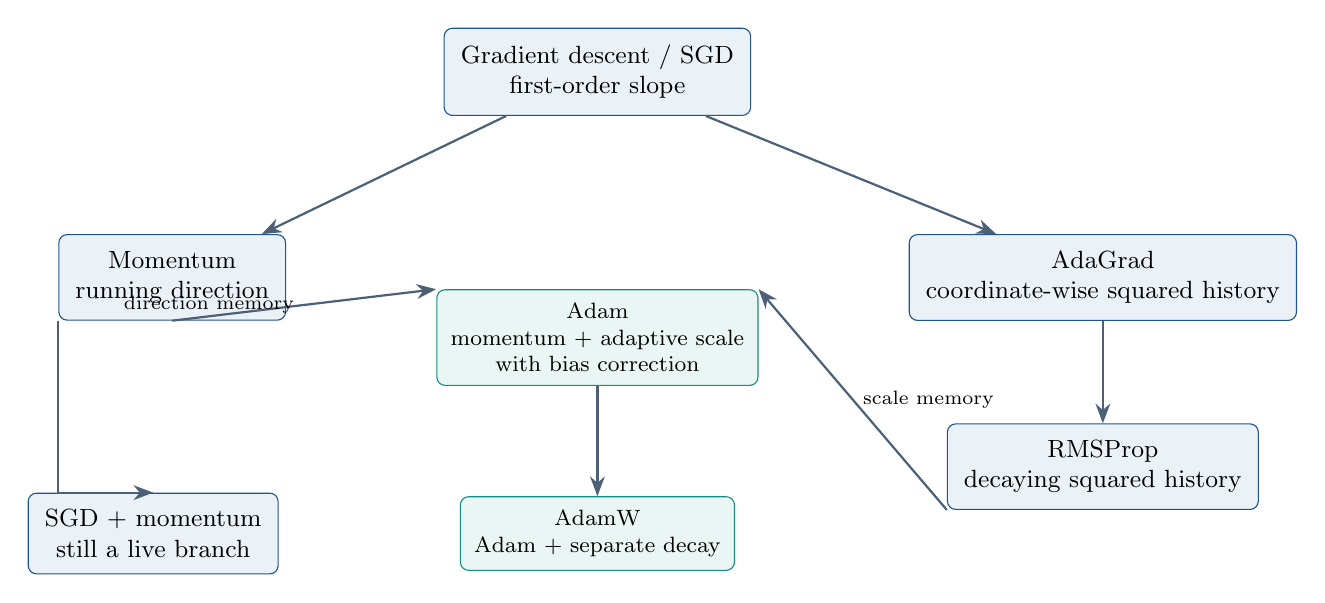
\begin{tikzpicture}[node distance=13mm and 16mm]
\node[flow] (gd) {Gradient descent / SGD\\first-order slope};
\node[flow,below left=15mm and 20mm of gd] (mom) {Momentum\\running direction};
\node[flow,below right=15mm and 20mm of gd] (ada) {AdaGrad\\coordinate-wise squared history};
\node[flow,below=13mm of ada] (rms) {RMSProp\\decaying squared history};
\node[yesbox,below=22mm of gd] (adam) {Adam\\momentum + adaptive scale\\with bias correction};
\node[yesbox,below=14mm of adam] (adamw) {AdamW\\Adam + separate decay};
\node[flow,left=23mm of adamw] (sgdm) {SGD + momentum\\still a live branch};
\draw[arr] (gd)--(mom);
\draw[arr] (gd)--(ada);
\draw[arr] (ada)--(rms);
\draw[arr] (mom.south) -- node[left,font=\scriptsize]{direction memory} (adam.north west);
\draw[arr] (rms.south west) -- node[right,font=\scriptsize]{scale memory} (adam.north east);
\draw[arr] (adam)--(adamw);
\draw[arr] (mom.south west) |- (sgdm.north);
\end{tikzpicture}}
\caption{The original first-order genealogy: retaining direction, adapting coordinate scales, combining both, then decoupling regularisation. SGD with momentum remains a separate useful branch.}
\end{figure}

\begin{center}
\small
\begin{tabularx}{.97\linewidth}{@{}L{.18\linewidth}L{.26\linewidth}YY@{}}
\toprule
\textbf{Step / branch} & \textbf{What changed} & \textbf{Problem targeted} & \textbf{New trade-off} \\
\midrule
SGD $\to$ momentum & Store recent direction & Slow progress / zig-zagging & Overshoot and momentum tuning \\
AdaGrad $\to$ RMSProp & Forget old squared gradients & AdaGrad's shrinking effective steps & Scale-decay tuning \\
Momentum + RMSProp $\to$ Adam & Combine direction, scale, bias correction & Unequal gradient scales & Two state vectors \\
Adam $\to$ AdamW & Decouple parameter shrinkage & L2 enters Adam's scaling & Separate decay choice \\
Adam $\to$ Adafactor & Factor scale state & Optimiser memory & Approximate matrix scales \\
Momentum $\to$ Lion / Muon & Signed or orthogonalised updates & Different update geometry / memory & New tuning and assumptions \\
Gradient $\to$ curvature methods & Use slope changes and parameter coupling & Poor conditioning & More curvature compute / state \\
\bottomrule
\end{tabularx}
\end{center}

\subsection{Curvature-Aware Updates}
\label{sec:optimisation-newton-s-method-and-other-second-order-methods}
If you're trying to find the bottom of a valley, you don't just follow the slope, you look at the slope of the slope - are we bottoming out (I will take a smaller step) or topping off (time to take a large jump over the top of the hill).
The Hessian measures how slope changes.
Newton's method uses a local quadratic model rather than assuming that one global step size should work along every direction.
As introduced in \cref{subsec:la-hessian}, the Newton step solves
\[
    \underbrace{\nabla_\theta^2\mathcal L(\theta_t)}_{\text{Hessian: curvature and parameter coupling}}
    \underbrace{\Delta\theta_{\text{Newton}}}_{\text{proposed update}}
    =-
    \underbrace{\nabla_\theta\mathcal L(\theta_t)}_{\text{gradient}}
    ,\qquad
    \theta_{t+1}=\theta_t+\Delta\theta_{\text{Newton}}.
\]
Steep curvature suppresses the corresponding component of the update; flat positive curvature permits a larger one.
For an exact positive-definite quadratic and an exact solve, Newton reaches its minimum in one step, whereas gradient descent can zig-zag through a badly conditioned valley.
On a nonconvex loss, the Hessian can have negative eigenvalues, which causes the Newton direction to ascend.

\paragraph{Damped Newton} adds a positive diagonal term to the Hessian and can limit the update using a line search or trust region:
\[
    \underbrace{(\nabla_\theta^2\mathcal L(\theta_t)+\lambda I)}_{\text{curvature + damping}}
    \underbrace{\Delta\theta}_{\text{controlled step}}
    =-\nabla_\theta\mathcal L(\theta_t).
\]
For sufficiently large damping, the system becomes positive definite and the direction approaches a scaled negative gradient.
A small damping parameter trusts the quadratic curvature model more; a large one acts conservatively when that model is unreliable.

\begin{figure}[htbp]
\centering
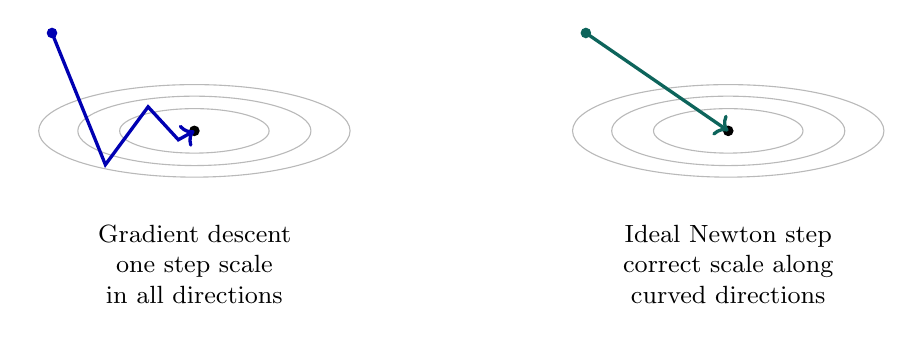
\begin{tikzpicture}[scale=1.13]
\begin{scope}[xshift=0cm]
\draw[gray!55] (0,0) ellipse (1.75 and .52);
\draw[gray!55] (0,0) ellipse (1.31 and .39);
\draw[gray!55] (0,0) ellipse (.84 and .25);
\fill (0,0) circle (1.7pt);
\draw[->,very thick,blue!70!black] (-1.6,1.1)--(-1.0,-.38)--(-.52,.27)--(-.18,-.10)--(0,0);
\fill[blue!70!black] (-1.6,1.1) circle (1.7pt);
\node[font=\small,align=center,text width=4.0cm] at (0,-1.5) {Gradient descent\\one step scale in all directions};
\end{scope}
\begin{scope}[xshift=6.0cm]
\draw[gray!55] (0,0) ellipse (1.75 and .52);
\draw[gray!55] (0,0) ellipse (1.31 and .39);
\draw[gray!55] (0,0) ellipse (.84 and .25);
\fill (0,0) circle (1.7pt);
\draw[->,very thick,teal!70!black] (-1.6,1.1)--(0,0);
\fill[teal!70!black] (-1.6,1.1) circle (1.7pt);
\node[font=\small,align=center,text width=4.0cm] at (0,-1.5) {Ideal Newton step\\correct scale along curved directions};
\end{scope}
\end{tikzpicture}
\caption{Illustrative paths on the same narrow quadratic valley. Newton uses cross-direction curvature to correct the step; stochastic, nonquadratic losses do not generally permit a single-step solution.}
\end{figure}

A dense Hessian has $N_{\text{parameters}}^2$ entries, so storing or factoring it is generally impractical for large neural networks.
Much of second-order optimisation research is therefore about \emph{which approximation is cheap enough to be useful}.

\paragraph{L-BFGS} avoids the full Hessian by keeping a short history of parameter changes and gradient changes, from which it builds an approximate inverse-curvature action.
It can be effective for smaller smooth problems with reliable objective evaluations; its gradient history is less reliable with very noisy mini-batches, and line searches may require extra forward/backward passes.

\paragraph{Gauss--Newton} is useful when the objective is built from residual errors.
For $\mathcal L(\theta)=\frac12\|r(\theta)\|^2$, it approximates the Hessian by
\[
\underbrace{\nabla_\theta^2\mathcal L(\theta)}_{\text{full Hessian}}
\quad\approx\quad
\underbrace{\left(\frac{\partial r}{\partial\theta}\right)^\top
\left(\frac{\partial r}{\partial\theta}\right)}_{\text{positive-semidefinite Gauss--Newton curvature}}.
\]
This drops second derivatives of the residuals and gives a positive-semidefinite curvature model, but the approximation may be poor far from a good fit.

\paragraph{Hessian-vector products} calculate $\nabla_\theta^2\mathcal L\,v$ without constructing the whole Hessian, allowing iterative linear solvers to approximate Newton-like directions.
The memory cost improves, but each iterative solve still requires additional differentiation work.

\paragraph{K-FAC} approximates layerwise curvature using Kronecker products of smaller matrices, giving an approximate natural-gradient direction based on Fisher information rather than the full Hessian.
\paragraph{Shampoo} uses matrix preconditioners along tensor dimensions so an update incorporates relationships within rows/columns or other tensor axes, rather than only elementwise scale.

\paragraph{Sophia} uses an inexpensive estimate of diagonal Hessian curvature and clips scaled coordinate updates.
It is more explicitly curvature-based than Adam, while deliberately giving up the cross-parameter information of a dense Newton step.

\begin{center}
\small
\begin{tabularx}{.97\linewidth}{@{}L{.19\linewidth}L{.27\linewidth}YY@{}}
\toprule
\textbf{Method} & \textbf{Geometry retained} & \textbf{Benefit} & \textbf{Cost / failure mode} \\
\midrule
Adam / RMSProp & Squared-gradient scale per coordinate & Cheap adaptive first-order updates & No cross-coordinate coupling \\
Newton / damped Newton & Full local Hessian & Corrects direction and scale for local curvature & Quadratic state; nonconvex curvature \\
L-BFGS & Recent changes in slope & No dense stored Hessian & Gradient noise / line-search overhead \\
Gauss--Newton & Jacobian-derived curvature & PSD approximation for residual objectives & Residual-model approximation \\
K-FAC / Shampoo & Structured layer/tensor preconditioner & Retains some coordinate interactions & Matrix state and operations \\
Sophia & Estimated diagonal Hessian & Curvature-adaptive scaling & No off-diagonal coupling; clipped steps \\
\bottomrule
\end{tabularx}
\end{center}


\section{Practical Points}

\subsection{Learning-Rate Schedules}
\label{sec:optimisation-learning-rate-schedules-and-warmup}
We can schedule Larning rate changes within a training run:
\begin{itemize}
    \item \textbf{Warmup} increases it gradually while gradient scales and optimiser state settle,
    \item \textbf{decay} reduces later changes,
    \item \textbf{cosine} decay changes it smoothly,
    \item \textbf{plateau} schedules react to a monitored metric
    \item \textbf{inverse-square-root}, 
\end{itemize}


\figpdf[.83\textwidth]{learning_rate_schedules}{Common relative learning-rate schedules: warmup, constant rate, cosine decay and a discrete step decay. The schedule is part of the optimiser, not a cosmetic setting.}



\subsection{Gradient Clipping}
A large gradient can cause instability in the loss function, and so we often clip off the tops of gradients to make sure they're always less than a threshold. 

\paragraph{Global-Norm } scales the entire gradient when its norm exceeds a threshold:
\[
    \underbrace{g_t^{\text{clipped}}}_{\text{gradient passed to optimiser}}
    =
    \underbrace{g_t}_{\text{computed gradient}}
    \min\!\left(1,\frac{\underbrace{c}_{\text{maximum norm}}}{\|g_t\|+\epsilon}\right).
\]
Unlike clipping each coordinate separately, global-norm clipping preserves the gradient's direction when it is clipped.

\begin{calloutpractical}
    For mixed-precision training, unscale gradients before clipping so the threshold applies to their real scale.
\end{calloutpractical}

\subsection{Gradient Accumulation}
\label{sec:optimisation-gradient-accumulation-and-mixed-precision}
Accelerator memory can limit the number of examples resident during one forward/backward pass.
\textbf{Gradient accumulation} runs several microbatches, adds or averages their gradients and updates parameters once:
\[
\underbrace{N_{\text{effective batch}}}_{\text{examples per update}}
=
\underbrace{N_{\text{microbatch}}}_{\text{resident examples}}
\times
\underbrace{N_{\text{accumulation steps}}}_{\text{passes per update}}
\times
\underbrace{N_{\text{data-parallel workers}}}_{\text{parallel workers}}.
\]
For a mean loss, each microbatch contribution must be weighted so the accumulated gradient represents the intended effective-batch average.
Accumulation reduces peak activation memory.

\begin{figure}[htbp]
\centering
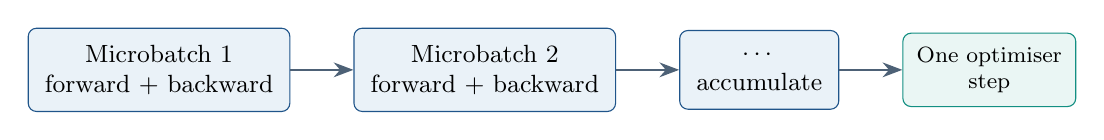
\begin{tikzpicture}[node distance=8mm and 8mm]
\node[flow] (m1) {Microbatch 1\\forward + backward};
\node[flow,right=of m1] (m2) {Microbatch 2\\forward + backward};
\node[flow,right=of m2] (mk) {$\cdots$\\accumulate};
\node[yesbox,right=of mk] (step) {One optimiser\\step};
\draw[arr] (m1)--(m2);
\draw[arr] (m2)--(mk);
\draw[arr] (mk)--(step);
\end{tikzpicture}
\caption{Original accumulation data flow: several smaller backward passes contribute to one effective-batch gradient and one parameter update.}
\end{figure}
\begin{calloutmemoryhook}
Accumulation reduces each batches memory.
\end{calloutmemoryhook}

\subsection{Mixed precision} performs suitable computation and storage in lower precision while keeping numerically sensitive quantities, often optimiser state, at higher precision.
FP16 offers more precision than BF16 but a much narrower exponent range.
BF16 tolerates a larger dynamic range, often avoiding the need for FP16-style loss scaling.
FP16 loss scaling temporarily multiplies the loss to keep small gradients representable, then unscales gradients before clipping and updating.
Lower precision usually reduces activation memory and bandwidth, but it does not guarantee a proportional speed-up if the workload is limited by launches, communication or unsupported operations (see the hardware chapter).

\begin{calloutmemoryhook}
    Mixed precision reduces bytes per tensor value.
\end{calloutmemoryhook}

\subsection{Diagnosing Problems}

\begin{center}
    \small
    \begin{tabularx}{.96\linewidth}{@{}L{.29\linewidth}YY@{}}
    \toprule
    \textbf{Observed behaviour} & \textbf{Likely variable to test} & \textbf{Interpretation / measurement} \\
    \midrule
    Loss diverges or oscillates & Learning rate, warmup, clipping & Inspect gradient/update norms and non-finite values \\
    Loss falls slowly in a narrow valley & Momentum or curvature scaling & Compare validation loss per unit compute \\
    Early progress, then stalls & Schedule; AdaGrad state; batch size & Compare effective learning rates and noise \\
    GPU memory exhausted & Microbatch, accumulation, precision, optimiser state & Separate activation, parameter and optimiser-state memory \\
    Training improves, validation degrades & Decay, data, regularisation, early stopping & Generalisation problem, not necessarily optimiser failure \\
    \bottomrule
    \end{tabularx}
\end{center}

\begin{calloutdegreeofexperiment}
Vary optimiser, learning-rate schedule, batch size, momentum/scale decay, gradient clipping, numerical precision, accumulation, weight decay and which parameter groups use each update rule.
\end{calloutdegreeofexperiment}

\section{Full Training Loop}
\label{sec:optimisation-the-full-training-loop}
The mathematical and systems choices above decompose to:
\begin{lstlisting}
optimizer.zero_grad()           # clear previous gradients
for inputs, targets in train_loader:
    predictions = model(inputs) # forward pass (optionally BF16/FP16)
    loss = loss_fn(predictions, targets) / accumulation_steps
    loss.backward()              # accumulate gradients

    if accumulation_boundary or final_batch:
        if FP16 loss scaling:
            unscale_gradients()
        clip_grad_norm_(model.parameters(), max_norm)
        optimizer.step()        # update parameters (AdamW decay here)
        optimizer.zero_grad()   # reset accumulated gradients
        scheduler.step()        # if scheduled per update
\end{lstlisting}
\textbf{Accumulation} delays the optimiser step until several backward passes have contributed gradients.
\textbf{Clipping} acts on the accumulated, unscaled gradients immediately before the optimiser step.
\textbf{Mixed precision} changes the forward/backward numerical representation.
FP16 may require loss scaling, while BF16 generally does not.
A scheduler is advanced after successful updates, per epoch or per validation metric according to its definition.
\chapter{Training Stability}
\label{chap:stability}
Now that we have covered architectures and optimisation methods, in theory we can design models which converge.
However, in practice, these things are very delicate and we need to carefully tune our design according to our chosen architecture, optimisation method and other design choices.

\section{Initialisation}
\label{sec:Initialisation}
A deep network repeatedly applies an update, and so an intuitive question is \textit{where should we start?}.
Because forward activations and backward updates can grow or shrink layer after layer, any instabilities compound and explode/zero, rather than cancelling out.

Zero-initialising all weights in a symmetric hidden layer prevents neurons from differentiating because equivalent units receive equivalent updates.
So, we introduce randomness to break the symmetry, and deploy variance scaling to keep the starting signal numerically usable.

\subsection{Xavier / Glorot and He / Kaiming Initialisation}
\label{sec:stability-xavier-glorot-and-he-kaiming-initialisation}
For a dense layer, common Gaussian starting variances are
\begin{align}
    \theta_{ij,\mathrm{Xavier}}
    &\sim
    \mathcal N\!\left(0,
    \underbrace{\frac{2}{N_{\text{inputs}}+N_{\text{outputs}}}}_{\text{balance forward/backward scale}}
    \right),\\
    \theta_{ij,\mathrm{He}}
    &\sim
    \mathcal N\!\left(0,
    \underbrace{\frac{2}{N_{\text{inputs}}}}_{\text{compensate ReLU half-zeroing}}
    \right).
\end{align}
Xavier is a common starting point for linear/tanh-like activations; He/Kaiming is designed around ReLU-like activations.
These are approximate signal-scale arguments, not guarantees that training remains well conditioned.

\begin{calloutpractical}
    ReLU-like activation: start with He/Kaiming; linear or tanh-like activation: Xavier/Glorot is a common baseline.
\end{calloutpractical}

\section{Normalisation}
\label{sec:normalisation}
Normalisation methods mainly differ in \textbf{which axes define the statistic}.
\figpdf[.89\textwidth]{normalization_axes}{BatchNorm and LayerNorm normalise different slices of an activation tensor.}

For $N_{\text{values}}$ values in the selected normalisation group:
\[
    \underbrace{\hat u_i}_{\text{centred/scaled value}}
    =
    \frac{
     u_i-\overbrace{\frac{1}{N_{\text{values}}}\sum_j u_j}^{\mu_{\text{group}}}
    }{
    \sqrt{
    \underbrace{\frac{1}{N_{\text{values}}}\sum_j(u_j-\mu_{\text{group}})^2}_{\sigma^2_{\text{group}}}
    +\epsilon
    }}.
\]
A learned scale and optional shift can restore useful amplitude/offset after normalisation.

\subsection{Batch Normalisation}
\label{subsec:stability-batch-normalisation}
BatchNorm averages across examples for corresponding features/channels during training and usually uses running training statistics at inference.
It can improve optimisation, but tiny or nonrepresentative batches make its reference statistics noisy or mismatched.
For example: In a house price prediction model, we normalise the \texttt{neighbour\_house\_price} feature to the average of the other houses in the batch.

\subsection{Layer Normalisation}
\label{subsec:stability-layer-normalisation}
LayerNorm averages within each example/token across a chosen feature set, so its statistics do not depend on unrelated examples in the batch.
This is why it fits sequence models with variable or small batch sizes well.
For example, In a house price prediction model, we may average all the input features of one example.

\subsection{RMSNorm}
\label{subsec:stability-rmsnorm}
RMSNorm controls vector magnitude without subtracting the mean:
\[
    \operatorname{RMSNorm}(h)_i
    =
    \theta_{\text{scale},i}
    \frac{h_i}{
    \sqrt{\frac{1}{N_{\text{features}}}\sum_j h_j^2+\epsilon}}
    .
\]
It is cheaper than full centring-and-scaling and is common in modern language models.

\begin{table}[htbp]
    \centering
    \small
    \begin{tabularx}{\linewidth}{@{}L{.19\linewidth}YYY@{}}
    \toprule
     & BatchNorm & LayerNorm & RMSNorm \\
    \midrule
    Statistics over & Batch, per feature/channel & Features within one example/token & Features within one example/token \\
    Subtract mean? & Yes & Yes & No \\
    Scale by & Standard deviation & Standard deviation & Root mean square \\
    Depends on other examples? & During training, yes & No & No \\
    \bottomrule
    \end{tabularx}
    \caption{Normalisation methods.}
\end{table}

These methods do not generally whiten cross-feature covariance; whitening is separated in \cref{sec:representation-whitening-pca-and-zca,sec:representation-whitening-versus-normalisation}.

\section{Regularisation}
Another method of improving stability is to penalise unstable changes within the model. 
For example, we may want to penalise parameter updates which are very large, because these \textit{can} lead to gradient explosions.  
\label{sec:stability-regularisation-l1-and-l2}
A regularised objective exposes the trade-off directly:
\[
    \underbrace{\mathcal L_{\text{total}}(\theta)}_{\text{what optimisation sees}}
    =
    \underbrace{\mathcal L_{\text{data}}(\theta)}_{\text{fit observations}}
    +
    \underbrace{\lambda R(\theta)}_{\text{parameter preference}}.
\]
L2 uses $R(\theta)=\|\theta\|_2^2$ and usually shrinks parameters smoothly.
L1 uses $R(\theta)=\|\theta\|_1$ and can drive coefficients exactly to zero.
Elastic Net combines both.
The interpretation depends on parameterisation, so ``small weights'' is not universally the same as ``simple realised function''.

\begin{calloutintuition}
    L1 is basically feature selection when individual weights map cleanly to input features.
    L2 shrinks rather than deletes them.
\end{calloutintuition}

The Bayesian MAP view is in \cref{sec:foundations-maximum-likelihood-and-maximum-a-posteriori-estimation}.
For Adam, decoupled weight decay changes the update relative to putting an L2 gradient inside Adam; see \cref{sec:optimisation-adamw-decouple-weight-decay-from-gradient-adaptation}.

\subsection{Dropout}
\label{sec:stability-dropout-and-stochastic-regularisation}
In inverted dropout, each activation is randomly kept with probability $1-p_{\text{drop}}$ and rescaled so its conditional expectation is unchanged:
\[
    \tilde h_j
    =
    \underbrace{\frac{m_j}{1-p_{\text{drop}}}}_{\text{random keep + expectation-preserving scale}}h_j,
    \qquad
    m_j\sim\operatorname{Bernoulli}(1-p_{\text{drop}}).
\]
Dropout discourages dependence on one exact active pathway, but too much stochasticity can make optimisation unnecessarily difficult.
It is disabled at inference.

\section{Augmentation}
\label{sec:stability-data-augmentation-and-symmetry-assumptions}
Augmentation asserts that a transformation should preserve or predictably transform the target.
A horizontal flip may preserve animal identity but invert left/right anatomy, time reversal may violate causality in a physical signal.
Augmentation is an inductive-bias choice, not free extra data.
See \cref{sec:nfl-inductive-bias-the-assumptions-that-make-learning-possible}.




\chapter{Evaluation Methods}
\label{chap:evaluation}
To evaluate a model, we look beyond the loss function. 
There are a few reasons for this, and that largest is simply that most evaluation methods are \textit{not} differentiable.
Therefore our most useful and expressive evaluation metrics (a suite of error representations) cannot be used during training.
We can use them afterwards though.

\section{Classification Evaluation}
\label{sec:evaluation-classification-evaluation-the-confusion-matrix}
For binary classification, predictions fall into true positive (TP), false positive (FP), true negative (TN) and false negative (FN).
\subsection{Confusion Matrix}
\begin{center}
    \small
    \begin{tabular}{@{}lcc@{}}
    \toprule
     & Actual positive & Actual negative \\
    \midrule
    Predicted positive & TP & FP \\
    Predicted negative & FN & TN \\
    \bottomrule
    \end{tabular}
\end{center}
Accuracy $(\mathrm{TP}+\mathrm{TN})/N_{\text{examples}}$ can hide rare-class failure because the majority class dominates the count.

\subsection{Precision, Recall and F1}
\label{sec:evaluation-precision-recall-and-f1}
\begin{align}
    \underbrace{P}_{\text{precision: correctness of alerts}}
    &=\frac{\mathrm{TP}}{\mathrm{TP}+\mathrm{FP}},\\
    \underbrace{R}_{\text{recall: coverage of positives}}
    &=\frac{\mathrm{TP}}{\mathrm{TP}+\mathrm{FN}},\\
    F_\beta
    &=(1+\beta^2)\frac{PR}{\beta^2P+R}.
\end{align}
Larger $\beta$ weights recall more strongly and smaller positive $\beta$ weights precision more strongly.
F1 ignores TN directly, so it is not automatically suitable when correctly rejecting negatives is itself important.

\begin{calloutspecialcase}
    The $F_1$ score is $F_\beta$ with $\beta=1$.
\end{calloutspecialcase}


\subsection{ROC curves, AUC-ROC and Precision--Recall}
\label{sec:evaluation-roc-curves-auc-roc-and-precision-recall}
The Receiver Operating Characteristic (ROC) curves compares true-positive rate against false-positive rate at different thresholds.
ROC-Area-Under-Curve (AUC) is the probability that a random positive is ranked above a random negative.

\figpdf[.9\textwidth]{roc_precision_recall}{ROC and precision--recall curves expose different threshold trade-offs.}

For rare events, a small false-positive rate can still create many more false alerts than true alerts.
Precision--Recall curves expose that directly, so rare-event systems should not rely on accuracy or ROC-AUC alone.

\begin{calloutpractical}
    Rare positives: report precision, recall and a precision--recall curve, then choose threshold from false-alarm versus miss cost.
\end{calloutpractical}


\section{Folded Validation}
\label{sec:evaluation-cross-validation-and-fold-choice}
As ML practitioners, we like to get statistical answers to our questions, and yet this model evaluation section trains one model and evaluates once with multiple metrics.
This is \textit{not} a strong statistical methodology, and so we train repeats on subsets of the data. 
These subsets are folds, and each fold is validated once while the others train the model.

The mean fold score is
\[
    \bar s
    =
    \frac{1}{N_{\text{folds}}}
    \sum_{i=1}^{N_{\text{folds}}}
    \underbrace{s_i}_{\text{score on held-out fold }i}.
\]
\begin{calloutpractical}
    Fold scores are correlated because their training sets overlap.
\end{calloutpractical}

\begin{figure}[htbp]
    \centering
    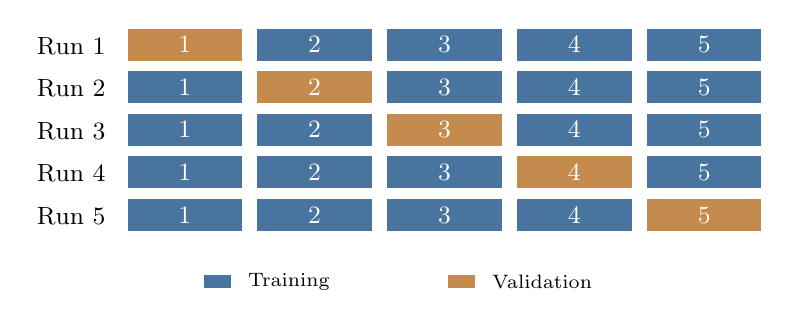
\begin{tikzpicture}[x=.97cm,y=.54cm]
    \foreach \r in {0,...,4}{
    \node[anchor=east,font=\small] at (-.16,-\r) {Run \the\numexpr\r+1\relax};
    \foreach \c in {0,...,4}{
    \ifnum\c=\r \fill[amber!85] (\c*1.7,-\r-.35) rectangle ++(1.5,.75);
    \else \fill[deepblue!82] (\c*1.7,-\r-.35) rectangle ++(1.5,.75);\fi
    \node[white,font=\small] at (\c*1.7+.75,-\r+.02) {\the\numexpr\c+1\relax};}}
    \fill[deepblue!82] (1,-5.7) rectangle ++(.35,.3);
    \node[anchor=west,font=\scriptsize] at (1.45,-5.55) {Training};
    \fill[amber!85] (4.2,-5.7) rectangle ++(.35,.3);
    \node[anchor=west,font=\scriptsize] at (4.65,-5.55) {Validation};
    \end{tikzpicture}
    \caption{Five-fold cross-validation: each fold is held out once.}
\end{figure}
    
\begin{tabularx}{\linewidth}{@{}L{.24\linewidth}YY@{}}
    \toprule
    Split strategy & Problem it Solves & Main leakage controlled \\
    \midrule
    Random K-fold & Examples are approximately independent and similarly distributed & Dependence on one arbitrary split \\
    Stratified K-fold & Class proportions vary strongly & Unrepresentative class balance \\
    Group K-fold & Repeated measurements share subject/run/instrument identity & Same group appearing on both sides \\
    Forward / time-series split & Future prediction & Training on future observations \\
    Nested CV & Hyperparameter selection with limited data & Reusing selection folds for final assessment \\
    \bottomrule
\end{tabularx}

\begin{calloutpractical}
Split by the independent unit: keep repeated measurements from one subject/run together, and preserve time order for forecasting.
\end{calloutpractical}


\section{Ranking metrics}
\label{sec:evaluation-retrieval-and-ranking-metrics}

\paragraph{Recall@K.}
If $N_{\text{relevant}}$ items exist and $N_{\text{relevant in top K}}$ survive the first stage,
\[
    \underbrace{\operatorname{Recall@K}}_{\text{candidate coverage}}
    =
    \frac{N_{\text{relevant in top K}}}{N_{\text{relevant}}}.
\]
A downstream reranker cannot recover an item that retrieval never produced.

\paragraph{MRR.}
Mean Reciprocal Rank rewards putting the first relevant result near the top:
\[
    \operatorname{MRR}
    =
    \frac{1}{N_{\text{queries}}}
    \sum_q
    \frac{1}{\underbrace{\operatorname{rank}_{q,\text{first relevant}}}_{\text{where useful information first appears}}}.
\]

\paragraph{NDCG.}
Discounted Cumulative Gain gives top positions more weight and allows graded relevance:
\[
    \underbrace{\operatorname{NDCG@K}}_{\text{normalised ranking quality}}
    =
    \frac{
    \sum_{r=1}^{K}
    \frac{2^{\operatorname{relevance}_r}-1}{\log_2(r+1)}
    }{
    \underbrace{\operatorname{IDCG@K}}_{\text{best possible ordering for this query}}
    }.
\]
The logarithmic discount is why swapping ranks 1 and 2 matters much more than swapping ranks 101 and 102.
\figpdf[.76\textwidth]{ndcg_discount}{NDCG's position discount falls quickly near the top, so high-ranking mistakes receive most of the metric weight.}

\begin{calloutpractical}
Evaluate candidate generation with coverage-oriented metrics such as Recall@K, then evaluate the later ordering with NDCG/MRR; one scalar for the whole funnel can hide which stage failed.
\end{calloutpractical}

\section{Generative Evaluation}
\label{sec:evaluation-generative-and-rag-evaluation}
\subsection{Golden Dataset}
A \textbf{golden dataset} acts like a test suite. 
A perfect, human derived set of examples allows reruns whenever the system changes, in the style of unit tests in software engineering.
Because models have biases, \textbf{LLM as a Judge} is limited, and requires calibration, usually from a golden set.

\subsection{Rag Evaluation}
\textbf{RAGAS}-style evaluation focuses on context precision/recall, answer relevancy and faithfulness.
\textbf{HELM}-style benchmarking instead asks broader base-model capability questions across standardised scenarios.

\begin{calloutmemoryhook}
    For RAG, separate ``did we retrieve the evidence?'' from ``did the generator use the evidence correctly?''.
\end{calloutmemoryhook}

\section{A/B Testing (Online Evaluation)}
\label{sec:evaluation-online-experiments-and-ab-testing}
How do you know whether a model is actually better in practice than an alternative?
You compare them in the real-world setting. 
We need a statistically strong signal to justify rolling out an iteration, and so we use statistics to answer the question.

We turn the deployment into an experiment, testing the delta:
\[
    \underbrace{\widehat{\Delta}}_{\text{estimated treatment effect}}
    =
    \underbrace{\bar y_{\text{treatment}}}_{\text{new system}}
    -
    \underbrace{\bar y_{\text{control}}}_{\text{old system}}.
\]
\textbf{Persistent assignment}, such as a stable hash of user identity, keeps one user in one condition and avoids mixing treatment exposure.

The null hypothesis is commonly $H_0:\Delta=0$.
A p-value asks how extreme the observed statistic would be under the null.
The standard-error scaling in \cref{sec:foundations-confidence-intervals} provides a sample-size approximation called the \textbf{Minimum Detectable Effect} (MDE):
\[
    \underbrace{\operatorname{MDE}}_{\text{smallest reliably detectable effect}}
    \propto
    \frac{1}{\sqrt{N_{\text{independent cases}}}}
    \quad\text{(all else equal)}.
\]
Halving the target MDE therefore costs roughly four times as many independent observations under the same noise/decision assumptions.

\begin{center}
    \small
    \begin{tabularx}{.9\linewidth}{@{}L{.25\linewidth}YY@{}}
    \toprule
     & Test says no effect & Test says effect \\
    \midrule
    No real effect & Correct & Type I error \\
    Real effect & Type II error & Correct detection \\
    \bottomrule
    \end{tabularx}
\end{center}

Repeatedly checking an ordinary fixed-horizon p-value and stopping the first time it crosses a threshold changes the testing procedure and inflates false-positive risk.
Use a predeclared horizon or a sequential method whose stopping rule is part of the design.

Ranking systems can also use \textbf{interleaving}: mix candidates from two rankers into one list so the same user/context provides a sensitive relative comparison.
Interleaving is useful for direct ranker preference but does not replace product-level A/B metrics such as retention or revenue.

\begin{calloutdegreeofexperiment}
    Vary assignment unit, traffic split, metric, MDE, test duration, stopping rule, segmentation and whether competing ranking systems are compared by A/B assignment or interleaving.
\end{calloutdegreeofexperiment}

\chapter{Post-Training Generalisation}
\label{chap:Downstream Post-Training Generalisation}
Often, a model is trained (at great cost) and needs to either \textit{specialise} to a subsection of the data, which was under-represented in the training, or \textit{generalise} to a new, unseen set of data.
When designing this kind of procedure, we need to ask ourselves \textit{what is shared, what changed, and how much of the model should be allowed to adapt?}


\section{Transfer Learning}
\label{sec:adaptation-transfer-learning-reuse-what-the-model-has-learned}

When \textit{transferring} to a new task, the main design choice is how much of the pretrained model we allow to change.

\begin{calloutmemoryhook}
    In post-training generalisation, overfitting is basically forgetting.
\end{calloutmemoryhook}

A model is \textbf{tuned} when training is continued from where the main training ended, normally with some carefully curated dataset.
For example, an image model may be found online, and further trained on a curated dataset of images in the style of Disney Animations, leading to a model which has \textit{specialised} in Disney's style, while retaining a lot of the general image model capabilities of the parent model.

A \textbf{Prediction Head} is a small layer on the end of a model which is added to handle a specific task. 
For example, imagine training a model to predict house prices and then wanting to predict the probability of a house selling in the next year. 
The problems share a lot of information, and so it may be worth just replacing the final layer of the house-price model and training just that layer on the new probability-of-sale data.

\textbf{Negative transfer} means that your post-trained model performs worse than your pre-trained model.

\begin{calloutmemoryhook}
    The word \textit{Fine-Tuning} should never have been invented, it just means \textit{continued training on custom data}.
\end{calloutmemoryhook}

\begin{table}[htbp]
    \centering
    \small
    \begin{tabularx}{\linewidth}{@{}L{.19\linewidth}YYY@{}}
    \toprule
    Strategy & What changes? & Main trade-off & Applications \\
    \midrule

    \textbf{Frozen}
    &
    The main model is kept the same, and a small secondary model is duct-taped onto the end, creating a specialised \textit{prediction head}.
    &
    Very cheap to train and retains the original representations, but the main model cannot adapt to the new task.
    &
    Small datasets where the pretrained features are already useful. E.g.\ adding a classifier to a pretrained image encoder.
    \\

    \addlinespace
    \textbf{Fully Tuned}
    &
    The entire model's training is continued on the new dataset. A prediction head is optional.
    &
    Maximum flexibility but highest cost, greater risk of overfitting.
    &
    Large, specialised datasets or substantial domain shifts. E.g.\ adapting a general image model to medical imaging.
    \\

    \addlinespace
    \textbf{Partially Tuned}
    &
    A prediction head is added, and a subset of the pretrained layers are also further trained, allowing the main model to specialise.
    &
    Balances adaptation against training cost, but performance depends on which layers are unfrozen.
    &
    Tasks where general low-level features remain useful but higher-level representations need adapting. E.g.\ retraining the final CNN blocks for a new classification task.
    \\

    \addlinespace
    \textbf{Efficiently Tuned}
    &
    Special, highly efficient methods of continuing training which only train a small number of parameters.
    &
    Much lower trainable-parameter and optimiser-memory cost, but constrains how the model can adapt. Total compute savings depend on the method.
    &
    Adapting large models under limited memory or maintaining many specialised versions of one base model. E.g.\ LoRA fine-tuning of an LLM.
    \\

    \bottomrule
    \end{tabularx}
    \caption{Transfer learning is a continuum of adaptation capacity, trading training cost against the freedom to specialise pretrained representations.}
\end{table}


\subsection{Domain Adaptation}
\label{sec:adaptation-domain-adaptation-the-data-distribution-changes}
It is useful to think of domain adatation as \textit{which probability distribution (or combination) changed?}
\begin{align}
    \underbrace{P_S(x)\ne P_T(x),\;P_S(y\mid x)=P_T(y\mid x)}_{\text{covariate shift: inputs change, rule stays}},\\
    \underbrace{P_S(y)\ne P_T(y),\;P_S(x\mid y)=P_T(x\mid y)}_{\text{label shift: class prevalence changes}},\\
    \underbrace{P_S(y\mid x)\ne P_T(y\mid x)}_{\text{concept shift: prediction rule changes}}.
\end{align}

Under covariate shift, examples can be \textbf{reweighted} to represent the target input distribution.
The input data itself can be adapted to fit the new distribution, like
\[
    \underbrace{\E_{P_T}[\ell]}_{\text{target risk}}
    =
    \underbrace{\E_{P_S}\!\left[
    \frac{P_T(x)}{P_S(x)}\ell(f(x),y)
    \right]}_{\text{source risk weighted toward target-like inputs}}.
\]
However, for small target regions (small classes, sparse prediction space, etc.) training on reweighted data just causes overfitting.

\figpdf[.8\textwidth]{domain_shift}{Synthetic covariate shift in one input coordinate. This feature could be reweighted as the distribution is just a transform (changed from Normal to another Normal).}

\begin{calloutmemoryhook}
    Reweighting can fix input-frequency shift but it cannot fix a changed input-to-label rule, and breaks under class imbalance.
\end{calloutmemoryhook}

\subsection{Summary}
\begin{calloutbias}
    \begin{tabularx}{\linewidth}{@{}L{.23\linewidth}YY@{}}
        \toprule
        Approach & Shared structure assumed & Failure to test \\
        \midrule
        Frozen transfer & Source representation retains target signal & Target feature was suppressed upstream \\
        Fine-tuning & Pretrained parameters are a useful starting point & Small target set overfits \\
        Domain invariance & Some task-relevant features persist across domains & Alignment mixes different classes \\
        Prototypical networks & Classes form meaningful embedding centroids & Classes are multimodal/overlapping \\
        MAML & New tasks resemble meta-training tasks & Task family changes substantially \\
        Zero-shot multimodal & Modalities share semantic geometry & Prompt/class semantics are ambiguous \\
        LoRA & Adaptation is approximately low rank & Task needs broad independent parameter changes \\
        \bottomrule
    \end{tabularx}
\end{calloutbias}

\section{Specialise: Zero-shot learning}
\label{sec:adaptation-zero-shot-learning-no-task-specific-labelled-examples}
Zero-shot learning is only really available to Large Language/Image Models, because few other models generalise as well as them.
It is done by changing the context that the model has available, rather than by changing weights.
For a shared image/text embedding, classification can be ``choose the text description with highest cosine similarity'':
\[
    \hat y
    =
    \argmax_j
    \underbrace{
    \frac{f_\theta(x)^\top g_\phi(t_j)}{\|f_\theta(x)\|_2\|g_\phi(t_j)\|_2}
    }_{\text{image--text directional similarity}}.
\]
Performance depends on the pre-training semantics, candidate class set and prompt wording.
Zero-shot does not mean zero prior knowledge, it assumes that the specific application exists within the pre-training dataset, and all we need to do is \textit{prompt better}.

\begin{calloutmemoryhook}
    Prompting changes context, while fine-tuning changes persistent parameters.
\end{calloutmemoryhook}


\section{Specialise: Few-shot learning}
\label{sec:adaptation-few-shot-learning-learn-from-very-few-examples}
Few shot learning allows us to curate a small dataset and conduct further training with it.
In the usual ``N-way K-shot'' terminology, an episode contains a small support set for each candidate class plus query examples for evaluation.
Few-shot learning is an approach, not a learning mechanism, so it can mean metric learning, gradient-based adaptation, frozen embeddings, or in-context prompting.

We reduce each class to a centroid:
\[
    \underbrace{c_{\text{class }j}}_{\text{class prototype}}
    =
    \frac{1}{N_{\text{support per class}}}
    \sum_{x_i\in S_j}f_\theta(x_i),
    \qquad
    \hat y_{\text{query}}
    =
    \argmin_j d\!\left(f_\theta(x_{\text{query}}),c_{\text{class }j}\right).
\]
This only works if the learned geometry makes same-class examples cluster in a transferable way.
\figpdf[.8\textwidth]{few_shot_prototypes}{Few labelled support examples define class prototypes; a query is classified by embedding-space proximity.}

\section{Generalise: Meta-learning and MAML}
\label{sec:adaptation-meta-learning-and-maml}
Meta-learning trains across tasks so that a new related task can be adapted quickly.
MAML makes that idea explicit by optimising query performance \emph{after} a task-specific support-set update:
\[
    \min_\theta
    \sum_{j=1}^{N_{\text{tasks}}}
    \mathcal L^{\text{query}}_j\!\left(
    \underbrace{
    \theta-\alpha\nabla_\theta\mathcal L^{\text{support}}_j(\theta)
    }_{\theta'_j:\ \text{one task-adaptation step}}
    \right).
\]
Exact differentiation through the inner update introduces second-order dependence.
First-order variants drop that cost.
The Hessian/second-order connection is in \cref{subsec:la-hessian,sec:optimisation-newton-s-method-and-other-second-order-methods}.



\section{Specialise: Parameter Efficient Continued-Training}
The general idea with Parameter Efficient Fine-Tuning (PEFT) is to avoid changing the large model instance.
Activations, optimiser states and the other backpropagation objects are very large to store in memory, and most specialisation problems do not require scale.
It's wasteful to train a full set of 1 billion parameters on 2000 examples!
So, we transform the weights into a low dimension using various transforming methods. 
We work in that lower dimensional space and then un-transform the results into the model.

\subsection{Low Rank Adapters (LoRA)}
\label{sec:adaptation-lora-a-parameter-efficient-adaptation-mechanism}
LoRA freezes a pretrained weight matrix and learns a low-rank update:
\[
    \underbrace{\theta'_{\text{weights}}}_{\text{adapted matrix}}
    =
    \underbrace{\theta_{\text{weights}}}_{\text{frozen pretrained matrix}}
    +
    \underbrace{\theta_{\text{up}}\theta_{\text{down}}}_{\Delta\theta:\ \text{low-rank update}}.
\]
This changes the bottleneck to the cost of dimension reduction/expansion:
\[
    \underbrace{\theta_{\text{down}}}_{\text{compress}}
    \in\R^{N_{\text{adaptation directions}}\times N_{\text{input features}}},
    \qquad
    \underbrace{\theta_{\text{up}}}_{\text{expand}}
    \in\R^{N_{\text{output features}}\times N_{\text{adaptation directions}}}.
\]
The parameter saving is:
\[
    \underbrace{N_{\text{adaptation directions}}
    \left(N_{\text{input features}}+N_{\text{output features}}\right)}_{\text{trainable LoRA parameters}}
    \quad\text{vs.}\quad
    \underbrace{N_{\text{input features}}N_{\text{output features}}}_{\text{full matrix parameters}}.
\]
The underlying assumption is that useful task adaptation lives in relatively few independent directions.
Low trainable-parameter count does not imply every training/inference cost shrinks proportionally.


\subsection{Quantised Low Rank Adapters (QLoRA)}
\label{subsec:adaptation-qlora}
QLoRA combines two different restrictions: keep the pretrained base model in a low-bit representation to save memory, while training LoRA adapters for task-specific change.
Conceptually,
\[
    \underbrace{\text{quantised frozen base}}_{\text{cheap storage}}
    +
    \underbrace{\text{trainable low-rank update}}_{\text{adaptation capacity}}.
\]
Quantisation and low-rank adaptation solve different bottlenecks, so they compose naturally.
Quantisation mechanics and their quality--memory trade-off are developed in \cref{sec:inference-quantisation}.

\begin{calloutmemoryhook}
    QLoRA compresses the frozen base, and LoRA restricts the trainable change.
\end{calloutmemoryhook}




\chapter{Unsupervised Learning}
\label{sec:unsupervised-learning}
Unsupervised learning attempts to learn from data without supplied task labels.
The choice of objective determines what the algorithm considers meaningful.
The main possibilities are: 
\begin{itemize}
    \item \textbf{Clustering} which observations belong together?,
    \item  \textbf{Density Estimation} where is probability mass?,
    \item \textbf{Latent Structure} can fewer factors explain the data?, and 
    \item \textbf{Anomaly Detection} which observations are unusual?.
\end{itemize}

\begin{figure}[htbp]
    \centering
    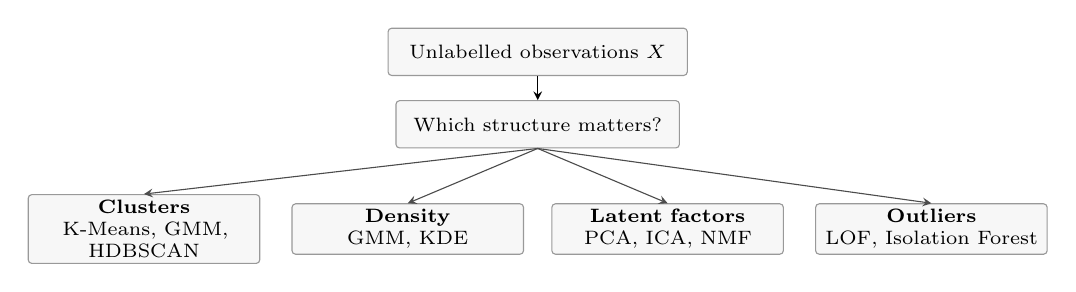
\begin{tikzpicture}[font=\scriptsize, >=stealth, node distance=3mm]
         \tikzset{ulbox/.style={draw=black!40,rounded corners=1.3pt,fill=black!3,align=center,minimum height=6mm,inner sep=2pt}}
         \node[ulbox,minimum width=38mm] (x) at (0,1.45) {Unlabelled observations $X$};
         \node[ulbox,minimum width=36mm] (q) at (0,.53) {Which structure matters?};
         \draw[->] (x)--(q);
         \node[ulbox,text width=28mm] (c) at (-5,-.8) {\textbf{Clusters}\\K-Means, GMM, HDBSCAN};
         \node[ulbox,text width=28mm] (d) at (-1.65,-.8) {\textbf{Density}\\GMM, KDE};
         \node[ulbox,text width=28mm] (l) at (1.65,-.8) {\textbf{Latent factors}\\PCA, ICA, NMF};
         \node[ulbox,text width=28mm] (a) at (5,-.8) {\textbf{Outliers}\\LOF, Isolation Forest};
         \foreach \n in {c,d,l,a}{\draw[->,black!70] (q.south) -- (\n.north);}
    \end{tikzpicture}
    \caption{Unsupervised learning taxonomy.}
    \label{fig:taxonomy}
\end{figure}


\section{Representation Similarity}
\label{sec:Representation Similarity foundations}
A cluster is a statement about \emph{representation similarity}, not a property of raw data alone.
Non-data based effects like representation choice and similarity metric choice decide clusters just as much as the raw data.
For observations $X\in\mathbb R^{N_{\text{samples}}\times N_{\text{features}}}$, changing representations (units, irrelevant features or standardisation) can change clusters.
And, for similarity metrics, we have many options
\begin{itemize}
    \item \textbf{Euclidean} distance preserves raw differences,
    \item \textbf{Cosine} compares direction rather than magnitude, 
    \item \textbf{Mahalanobis} measures separation after accounting for a chosen covariance geometry.
\end{itemize}

\begin{calloutmemoryhook}
    Clustering discovers structure between representations you choose in the distance metric you chose.
\end{calloutmemoryhook}


\begin{center}
    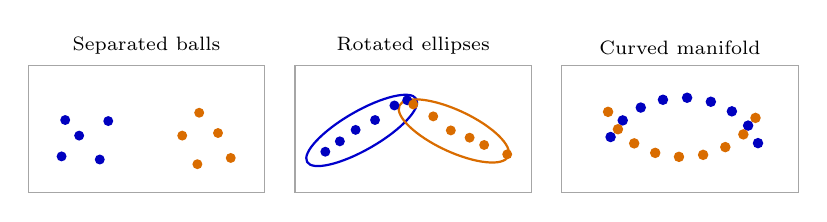
\begin{tikzpicture}[font=\scriptsize,x=.77cm,y=.66cm]
     \foreach \s/\name in {0/{Separated balls},4.4/{Rotated ellipses},8.8/{Curved manifold}} {
       \begin{scope}[shift={(\s,0)}]
        \draw[black!35] (0,0) rectangle (3.9,2.45);
        \node[anchor=south] at (1.95,2.48) {\name};
       \end{scope}
     }
     \foreach \x/\y in {.55/.7,.84/1.10,1.18/.64,.61/1.40,1.32/1.38,2.54/1.1,2.82/1.54,3.13/1.15,2.79/.55,3.34/.67}{\ifdim\x pt<2pt \fill[blue!75!black](\x,\y) circle(1.8pt); \else \fill[orange!85!black](\x,\y) circle(1.8pt);\fi}
     \begin{scope}[shift={(4.4,0)}]
      \draw[blue!80!black,thick,rotate around={30:(1.1,1.2)}] (1.1,1.2) ellipse (1.04 and .37);
      \draw[orange!85!black,thick,rotate around={-25:(2.62,1.19)}] (2.62,1.19) ellipse (.99 and .4);
      \foreach \x/\y in {.5/.79,.74/.99,1/1.21,1.32/1.4,1.64/1.68,1.85/1.78}{\fill[blue!75!black](\x,\y) circle(1.8pt);}
      \foreach \x/\y in {1.95/1.7,2.28/1.47,2.57/1.2,2.88/1.06,3.12/.92,3.5/.74}{\fill[orange!85!black](\x,\y) circle(1.8pt);}
     \end{scope}
     \begin{scope}[shift={(8.8,0)}]
       \foreach \a in {15,33,51,69,87,105,123,141,159}{\fill[blue!75!black] ({2+1.28*cos(\a)},{.65+1.18*sin(\a)}) circle (1.9pt);}
       \foreach \a in {195,213,231,249,267,285,303,321,339}{\fill[orange!85!black] ({2+1.28*cos(\a)},{1.86+1.17*sin(\a)}) circle (1.9pt);}
     \end{scope}
    \end{tikzpicture}
    \caption{Same two-colour objective, three geometries: centroids suit compact balls, covariance models tilted ellipses, and density/graph connections can represent curved groups.}
    \label{fig:geometries}
\end{center}

\section{Centroid Clustering}
\label{sec:kmeans}
\paragraph{K-Means} alternates two operations.
\begin{enumerate}
    \item assign every observation to its nearest \textbf{centroid},
    \item then \textbf{move} each centroid to the mean of its assigned observations.
\end{enumerate}
These operations preserve the within-cluster squared Euclidean error, so the algorithm converges to a local optimum, not necessarily the global one.
\[
    \underbrace{\min_{\{\mu_k\},\{c_i\}}\sum_{i=1}^{N_{\text{samples}}}\|x_i-\mu_{c_i}\|_2^2}_{\text{within-cluster squared distance}}
    \qquad\Longleftrightarrow\qquad
    \underbrace{c_i\gets\arg\min_k\|x_i-\mu_k\|_2^2}_{\text{assign}}
    \ \to\ 
    \underbrace{\mu_k\gets\operatorname{mean}_{i:c_i=k}(x_i)}_{\text{recentre}}.
\]

\paragraph{K-Means++} seeds centroids to spread them across the data, reducing poor initialisations.
Multiple seeds still matter because the objective is non-convex.
\paragraph{Mini-Batch K-Means} estimates centroid updates from subsets and therefore scales better to large datasets, at the cost of noisier, potentially less accurate solutions.
\paragraph{K-Medoids} uses actual observations as representatives and can use non-Euclidean dissimilarities.
It is less sensitive to extreme values than means, but often costs more to fit.

The basic iteration costs roughly $O(N_{\text{samples}}K N_{\text{features}})$ per pass, so the number of iterations and repeats determine the actual work needed.
Because errors are squared, a distant outlier can pull a mean markedly, and K-Means must assign that outlier to some cluster even when no group is credible.
Increasing $N_{\text{Clusters}}$ can reduce within-cluster error simply by spending more centroids, so a lower objective value does not by itself establish a more meaningful partition.


\begin{figure}[htbp]
    \centering
    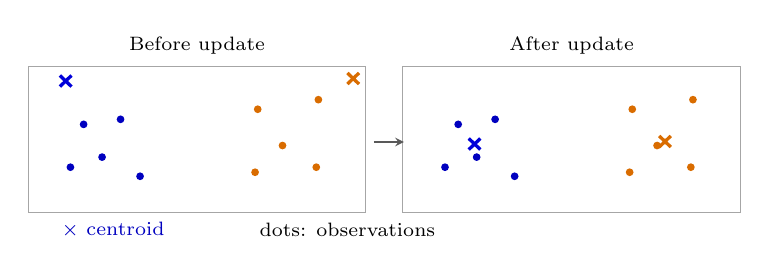
\begin{tikzpicture}[x=.67cm,y=.64cm,font=\scriptsize,>=stealth]
        \foreach \shift/\lab in {0/{Before update},7.1/{After update}}{
            \begin{scope}[shift={(\shift,0)}]
                \draw[black!35] (-.2,-.2) rectangle (6.2,2.7);
                \foreach \px/\py in {.6/.7,1.2/.9,.85/1.55,1.55/1.65,1.92/.52,4.1/.6,4.62/1.13,5.26/.7,4.15/1.85,5.3/2.04}{
                    \ifdim\px pt<3pt
                        \fill[blue!75!black] (\px,\py) circle (1.4pt);
                    \else
                        \fill[orange!85!black] (\px,\py) circle (1.4pt);
                    \fi
                }
                \node[anchor=south] at (3,2.75) {\lab};
            \end{scope}
        }
        \draw[blue!85!black,very thick] (.4,2.3)--(.62,2.52) (.4,2.52)--(.62,2.3);
        \draw[orange!85!black,very thick] (5.85,2.35)--(6.07,2.57) (5.85,2.57)--(6.07,2.35);
        \draw[blue!85!black,very thick] (8.15,1.05)--(8.37,1.27) (8.15,1.27)--(8.37,1.05);
        \draw[orange!85!black,very thick] (11.76,1.1)--(11.98,1.32) (11.76,1.32)--(11.98,1.1);
        \draw[->,black!65] (6.35,1.2)--(6.92,1.2);
        \node[blue!75!black,anchor=west] at (.25,-.55) {$\times$ centroid};
        \node[anchor=west] at (4.0,-.55) {dots: observations};
    \end{tikzpicture}
    \caption{K-Means updates centroids after nearest-centre assignments.}
    \label{fig:kmeans}
\end{figure}

\begin{calloutpractical}
    If groups are circular, nearest-centroid partitions are effective; elongated, curved, unequal-density or overlapping groups violate this bias.    
\end{calloutpractical}


\section{Probabilistic Clustering}
\label{sec:gmm}
\paragraph{Gaussian Mixture Model (GMM)}
Gaussian Mixture Models (GMM) work by dropping independent Gaussian distributions on the feature space and moving them (shifting mean and standard deviations) until they represent the clusters well.
because of the probability nature of these distributions, observations can have \emph{partial membership} in several groups.
The weighted components also define a probability density.
Unlike K-Means, GMM can model substantial overlap.
A fitted Gaussian component does not correspond to a meaningful physical class.
\[
    \underbrace{p(x)}_{\text{mixture density}}
    =\sum_{k=1}^{K}\underbrace{\pi_k}_{\text{component prevalence}}
    \underbrace{\mathcal N(x\mid\mu_k,\Sigma_k)}_{\text{component shape}},
    \quad \sum_k\pi_k=1;
    \qquad
    \underbrace{P(c_i=k\mid x_i)}_{\text{soft membership}}
    =\frac{\pi_k\mathcal N(x_i\mid\mu_k,\Sigma_k)}{\sum_j\pi_j\mathcal N(x_i\mid\mu_j,\Sigma_j)}.
\]
\paragraph{Expectation-Maximisation (EM)} is the optimisation process. 
It alternates between estimating how much each component explains every observation (E-step) and refitting component parameters using those fractional memberships (M-step).
Each exact EM iteration does not decrease the observed-data likelihood, but can converge to a poor local optimum.
The M-step provides a new mean and covariance,
\[
    \underbrace{\mu_k\gets\frac{\sum_i r_{ik}x_i}{\sum_i r_{ik}}}_{\text{membership-weighted centre}},\qquad
    \underbrace{\pi_k\gets\frac{\sum_i r_{ik}}{N_{\text{samples}}}}_{\text{component prevalence}},\qquad
    \underbrace{\Sigma_k\gets\frac{\sum_i r_{ik}(x_i-\mu_k)(x_i-\mu_k)^\top}{\sum_i r_{ik}}}_{\text{within-component covariance}},
\]
with $r_{ik}=P(c_i=k\mid x_i)$ from the E-step.
A point lying equally between two components has values near $(0.5,0.5)$, while a distant well-separated point tends towards a near-binary assignment.
This fractional accounting is the main difference from K-Means.


\subsection{Covariance}
\begin{itemize}
    \item \textbf{Spherical} covariance assumes equally shaped balls, 
    \item \textbf{Diagonal} covariance permits axis-aligned ellipses, 
    \item \textbf{Full} covariance permits rotated ellipses.
    It costs $O(KN_{\text{features}}^2)$ parameters and can overfit, 
    \item \textbf{Tied} covariance shares a shape across components.
\end{itemize}

\begin{calloutpractical}
    Choose $N_{\text{Clusters}}$ using held-out likelihood or complexity-aware criteria such as BIC as a density-model baseline, and separately test whether the assignments are stable and useful.    
\end{calloutpractical}

\begin{calloutspecialcase}
    With equal spherical covariances and vanishing variance, the dominant GMM component becomes the nearest mean.
    Hard assignments approach K-Means (under the corresponding objective assumptions).
\end{calloutspecialcase}

\begin{calloutmemoryhook}
    K-Means assigns a centre, and GMM assigns a probability distribution.
\end{calloutmemoryhook}

\section{Hierarchical clustering}
\label{sec:hierarchical}
\paragraph{Agglomerative Hierarchical Clustering} starts with one cluster per observation and repeatedly merges the closest pair of clusters.
It produces a \textbf{dendrogram} (think; tree roots), where the height of each merge records the chosen dissimilarity, and cutting the tree at different heights changes the clustering resolution without rerunning the merges.
The meaning of ``closest'' is set by \textbf{linkage}: 
\begin{itemize}
    \item \textbf{Single:} nearest pair (can chain via bridges), 
    \item \textbf{Complete:} farthest pair (favour compact groups), 
    \item \textbf{Average:}  mean pairwise distance, 
    \item \textbf{Ward:} smallest increase in within-cluster squared error (normally Euclidean).
\end{itemize}

Agglomerative methods avoid a single pre-specified $N_{\text{Clusters}}$ and expose nested structure, which is great for developers.
However, early incorrect merges cannot be undone.
Naive implementations require quadratic distance storage, often limiting use on very large datasets.
\paragraph{Divisive} hierarchical clustering reverses the construction (start with one cluster, recursively split), but is less commonly used.

\begin{center}
    \begin{minipage}{\linewidth}\centering
    \begin{tikzpicture}[x=.75cm,y=.50cm,font=\scriptsize,thick]
         \foreach \x/\lbl in {0/A,1/B,2/C,3/D,4/E,5/F}{\node at (\x,-.38) {\lbl};}
         \draw (0,0)--(0,1) --(1,1)--(1,0);
         \draw (.5,1)--(.5,2.7)--(2.5,2.7)--(2.5,1.35);
         \draw (2,0)--(2,1.35)--(3,1.35)--(3,0);
         \draw (4,0)--(4,.78)--(5,.78)--(5,0);
         \draw (4.5,.78)--(4.5,3.35)--(1.5,3.35)--(1.5,2.7);
         \draw[densely dashed,blue!70] (-.35,1.95)--(5.35,1.95);
         \node[anchor=west] at (5.55,1.95) {cut height};
         \node[anchor=east,rotate=90] at (-.50,1.55) {merge distance};
         \caption{The dendrogram preserves nested merges; changing the cut produces a different number of groups.}
    \end{tikzpicture}
    \label{fig:dendrogram}
    \end{minipage}
\end{center}


\section{Density Clustering}
\label{sec:density-clustering}
\paragraph{DBSCAN} defines a neighbourhood of radius $\varepsilon$ around each observation and marks a point as a \textbf{core} when it has at least $N_{\text{min points}}$ observations in that neighbourhood (typically counting itself).
Each datapoint within the radius is like a distance weighted vote on the density, generating clean transitions even where datapoints are sparse.
Connected core regions become clusters, nearby non-core points may be included as \textbf{border} points, and unassigned observations are \textbf{noise}.
It can find curved, irregular groups and reject isolated observations without choosing $N_{\text{Clusters}}$.
However, one global $\varepsilon$ struggles when meaningful groups have different densities, because a radius that merges a sparse group may also merge nearby dense groups.

\begin{center}
    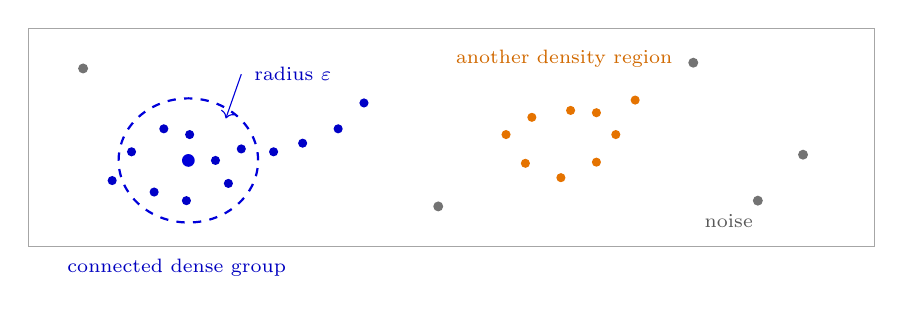
\begin{tikzpicture}[x=.82cm,y=.73cm,font=\scriptsize]
     \draw[black!35] (-.3,-.25) rectangle (12.8,3.55);
     \foreach \x/\y in {1/.9,1.3/1.4,1.8/1.8,2.2/1.7,2.6/1.25,2.8/.85,1.65/.70,2.15/.55,3/1.45,3.5/1.4,3.95/1.55,4.5/1.8,4.9/2.25}{\fill[blue!78!black] (\x,\y) circle (1.65pt);}
     \foreach \x/\y in {7.1/1.7,7.5/2.0,8.1/2.12,8.5/2.08,8.8/1.70,8.5/1.22,7.95/.95,7.4/1.2,9.1/2.3}{\fill[orange!90!black] (\x,\y) circle (1.65pt);}
     \foreach \x/\y in {.55/2.85,6.05/.45,10/2.95,11.7/1.35,11/0.55}{\fill[black!55] (\x,\y) circle (1.8pt);}
     \draw[blue!85!black,dashed,thick] (2.18,1.25) circle (1.08);
     \fill[blue!85!black] (2.18,1.25) circle (2.3pt);
     \draw[->,blue!85!black] (3.0,2.75)--(2.76,1.98);
     \node[anchor=west,blue!75!black] at (3.05,2.76) {radius $\varepsilon$};
     \node[blue!75!black] at (2,-.62) {connected dense group};
     \node[orange!82!black] at (8,3.02) {another density region};
     \node[black!65] at (10.55,.20) {noise};
    \end{tikzpicture}
    \caption{DBSCAN grows groups through core-point density connectivity, while leaving sufficiently isolated observations unassigned.}\label{fig:dbscan}
\end{center}

\paragraph{HDBSCAN} extends the density approach by constructing a hierarchy using density-sensitive (mutual-reachability) distances, then selecting clusters that persist over a range of density levels.
Its main practical controls are minimum cluster size and minimum samples.
Minimum size encodes how small a group is worth retaining, while increasing minimum samples usually makes the selection more conservative.
Smaller minimum cluster size admits more fine-grained groups but may label sampling fluctuations as discoveries.
Larger values favour coarser, more persistent structures.
A returned membership strength reflects the algorithm's notion of cluster persistence, not a calibrated posterior probability that the physical state is ``correct''.
Unlike DBSCAN, a single $\varepsilon$ is not the main global cut, though severe density variation and a poorly chosen representation remain problematic.
\paragraph{OPTICS} orders observations to reveal density-connected structure over several neighbourhood scales.
Generally, it's useful when a single DBSCAN radius is insufficient and a density ordering is itself informative.


\section{Spectral Clustering}
\textbf{Spectral Clustering} changes the problem from clustering points by their coordinates to clustering a graph by its connectivity.
Build a graph ($W_{ij}$) by joining observations (nodes) by their similarity (edges).
The graph may be fully connected, $\epsilon$-neighbourhood, or $k$-nearest-neighbour.
Sparse neighbour graphs avoid storing every pairwise connection.
The diagonal \textbf{degree matrix} stores each node's total connection strength by summing all its connections.
A \textbf{graph Laplacian} then compares this total connectivity with the individual connections in $W$, with many possible methods:
\begin{itemize}
    \item \textbf{Unnormalised:} $L=D-W$.
    \item \textbf{Symmetric normalised:} $L_{\mathrm{sym}}=I-D^{-1/2}WD^{-1/2}$.
    \item \textbf{Random-walk normalised:} $L_{\mathrm{rw}}=I-D^{-1}W$.
\end{itemize}

Take the smallest eigenvalued eigenvectors and stack them as
\[
    U\in\mathbb{R}^{N_{\mathrm{points}}\times N_{\mathrm{clusters}}}.
\]
Each row of $U$ is the original point expressed in graph-connectivity coordinates rather than feature coordinates.
Disconnected graph components give zero eigenvalues and weakly connected groups give corresponding low-eigenvalue directions.
For $L_{\mathrm{sym}}$, the rows of $U$ are commonly normalised before running K-Means on these new coordinates.

\begin{calloutintuition}
    In summary, make a similarity matrix and make a low rank reduction of it, and then do usual clustering methods on it.
\end{calloutintuition}

\begin{calloutpractical}
    For strong inter-cluster and weak intra-cluster connectivity, spectral clustering can recover non-convex groups that centroid methods miss.
\end{calloutpractical}

\begin{calloutpractical}
    The main choices are how similarity is defined, which edges are kept, which Laplacian is used, and how many eigenvectors/clusters are retained.
    Spectral clustering gains flexible cluster geometry, but building and eigendecomposing the similarity graph becomes expensive for large datasets.
\end{calloutpractical}

\section{Kernel Density Estimation (KDE)}
KDE places a smooth kernel at each observation and adds these contributions to estimate the full density without first assuming $N_{\text{Clusters}}$ Gaussian components.
For an isotropic kernel in $N_{\text{features}}$ dimensions, $\hat p(x)\propto \sum_i K((x-x_i)/h)/(N_{\text{samples}}h^{N_{\text{features}}})$; \textbf{bandwidth $h$} is the main smoothness choice.
Small $h$ gives a spiky density and large $h$ merges local structure; density estimation becomes substantially harder as dimensions increase, and naive query cost scales with the number of observations.

\section{Latent Factorisation}
\textbf{PCA} extracts orthogonal maximum-variance directions; the existing \emph{Data: Preprocessing} section already explains its eigenvector and whitening views.
\textbf{Independent Component Analysis (ICA)} seeks statistically independent sources rather than merely uncorrelated directions, typically relying on non-Gaussian independent components and an identifiable mixing model.
\textbf{Non-negative Matrix Factorisation (NMF)} approximates a non-negative data matrix as two non-negative factors, $X\approx WH$, encouraging additive, parts-based explanations; the components are generally not unique.
For neural nonlinear compression, see autoencoders in \emph{Model Family Overview} and VAEs in \emph{Generative Modelling}; neither reconstruction loss nor a smooth latent plot guarantees clusters useful for a downstream task.

\begin{center}
\begingroup\ULtight\small
\begin{tabular}{@{}p{.16\linewidth}p{.30\linewidth}p{.30\linewidth}p{.17\linewidth}@{}}
\hline
\textbf{Method} & \textbf{Assumption / structure} & \textbf{Use when} & \textbf{Main limitation}\\\hline
K-Means & Compact groups around means & Cheap flat partition of many points & Hard, nearly spherical groups\\
GMM / EM & Mixture of Gaussian densities & Overlap, uncertainty, density needed & Covariance and likelihood fragility\\
Hierarchical & Groups have useful nested merges & Explore scale and linkage & Cost; merges irreversible\\
DBSCAN & Dense connected sets + noise & Irregular shapes, explicit noise & Global density threshold\\
HDBSCAN & Stable density hierarchy & Density varies; abstention useful & Sensitivity to sampling/geometry\\
Spectral & Similarity graph has weak cuts & Manifold / graph-separated groups & Graph build and eigensolver\\
KDE & Smooth sum of local kernels & Low-dim density estimation & Bandwidth; high-dimensional cost\\
ICA / NMF & Independent sources / additive factors & Interpretable latent decomposition & Strong assumptions; ambiguity\\\hline
\end{tabular}
\ULtabcap{Primary inductive biases and decision boundaries; these algorithms answer different questions rather than forming a single ranking.}\label{tab:family}
\endgroup
\end{center}

\section{Anomaly detection without anomaly labels}\label{sec:anomaly}
An \textbf{anomaly score} ranks how unusual an observation is relative to the training distribution; it does not establish that the observation is faulty, harmful or causally exceptional.
A physical fault may occur in a dense region, while a legitimate new operating regime may appear as an isolated point.
\textbf{Isolation Forest} builds random partition trees and scores observations by how quickly they become isolated: unusual points tend to require fewer splits.
\textbf{Local Outlier Factor (LOF)} compares local density with nearby neighbours, identifying points that are sparse \emph{relative to their surroundings}; its neighbour count determines the scale of abnormality.
\textbf{GMM/KDE likelihood} can rank low-density points, but likelihood is not automatically a reliable anomaly score in high dimensions: density depends on representation/units, and high-likelihood regions need not match the distribution's typical set.
Autoencoder reconstruction error is another option; a high-capacity decoder can reconstruct some anomalous samples well and fail on legitimate but rare ones.

\begin{calloutmemoryhook}
Unusual under a model is not necessarily wrong in the world.
\end{calloutmemoryhook}
\subsection{Deployment threshold.}
If a review team can investigate only $B$ items per day, choose the top-$B$ scores or calibrate a threshold against a labelled review set or a representative reference period.
State the expected alert rate, missed-event cost and sensitivity to drift; do not describe a nominal contamination fraction as a known real-world fault prevalence.
The same evaluation problem occurs in \emph{Use Case: Real-Time Moderation}, where ranking, threshold and review capacity are separate design decisions.

\section{Evaluation: when there is no correct label}\label{sec:evaluation}
An internal clustering score measures whether the algorithm satisfies a geometric criterion, not whether the resulting groups correspond to meaningful physics or useful decisions.
The evaluation must distinguish \textbf{geometric fit}, \textbf{stability}, and \textbf{downstream value}.
\begin{center}
\begingroup\ULtight\small
\begin{tabular}{@{}p{.20\linewidth}p{.36\linewidth}p{.35\linewidth}@{}}
\hline
\textbf{Measure} & \textbf{What it rewards} & \textbf{Why it can mislead}\\\hline
Silhouette & Tight points separated from next-nearest cluster; $s_i=(b_i-a_i)/\max(a_i,b_i)$ & Prefers particular distance geometry; irregular dense groups may score poorly\\
Davies--Bouldin & Low within-group scatter compared with inter-centre separation (lower is better) & Inherits centroid/compactness assumptions\\
Log-likelihood & High probability assigned by density model to held-out data & High density is not semantic membership or guaranteed OOD detection\\
AIC / BIC & Likelihood balanced against model parameter count & Approximate selection assumptions; best density fit may not give best groups\\
Stability / ARI & Similar assignments under sampling, seeds or perturbations & A stable answer can still be arbitrary or irrelevant\\
Downstream utility & Improvement on retrieval, forecasting, fault detection, scientific discovery & Needs a well-designed external task; may leak labels into selection\\\hline
\end{tabular}
\ULtabcap{Evaluation criteria test different desiderata; no universal unsupervised score is a substitute for task validation.}\label{tab:metrics}
\endgroup
\end{center}

\subsection{Failure diagnostics.}
The most useful next step is usually a controlled intervention on the representation or the model assumption, not a more complicated algorithm.
\begin{center}
\begingroup\ULtight\small
\begin{tabular}{@{}p{.32\linewidth}p{.32\linewidth}p{.29\linewidth}@{}}
\hline
\textbf{Observed behaviour} & \textbf{Possible mechanism} & \textbf{Next experiment}\\\hline
Clusters change after feature scaling & A few units/features dominate distance & Inspect feature contribution; standardise or weight deliberately\\
K-Means gives one huge, one tiny group & Unequal density, outliers or poor $N_{\text{Clusters}}$ & Check seeds; try GMM or density clustering\\
GMM covariance nearly singular & Component fits one/few observations & Regularise; reduce dimension; compare covariance type\\
DBSCAN: nearly everything is noise & Neighbourhood too small for the sampling density & Revisit $\varepsilon$, min points and representation\\
Single linkage forms a long chain & Thin bridges connect distant groups & Compare average/complete/Ward linkage\\
Clusters align with collection date & Instrument or acquisition batch shift & Hold out dates/apparatus; inspect raw features\\
Only t-SNE produces separated islands & Projection exaggerates local gaps & Quantify clusters in the original embedding\\
\hline
\end{tabular}
\ULtabcap{Failure modes should trigger experiments that distinguish representation errors from algorithm assumptions.}\label{tab:failures}
\endgroup
\end{center}

\subsection{Internal geometry.}
In the silhouette expression, $a_i$ is an observation's average distance to its assigned cluster and $b_i$ the smallest average distance to another cluster.
A score near $1$ reflects separation under that distance, near $0$ an ambiguous boundary; it does not imply true discrete categories.
The elbow of K-Means inertia against $N_{\text{Clusters}}$ is only a heuristic: the cost always decreases or stays fixed as $N_{\text{Clusters}}$ increases, often without a distinct bend.
\subsection{Stability.}
Repeat fitted pipelines across seeds and bootstrap or subsampling splits, compare co-assignment relationships or matched partitions, and note how many points switch groups or become noise.
Adjusted Rand Index (ARI) compares assignments while being invariant to arbitrary cluster names; use it to compare repeat runs on a common set of observations, not to pretend unsupervised truth labels exist.
A stable cluster can still be an artefact of a fixed feature transformation or batch effect, so perturb the preprocessing and representation as well.
\subsection{Downstream tests.}
Evaluate a frozen unsupervised pipeline on held-out samples, a meaningful split by apparatus/time/source when relevant, and an application-specific task.
If labelled outcomes exist for external checking, keep them out of clustering, representation selection and hyperparameter tuning unless explicitly switching to a supervised selection protocol; otherwise claimed ``unsupervised'' performance can conceal label leakage.
The corresponding experiment-split and generalisation principles are in \emph{Evaluation, Validation and Model Selection}.

\begin{calloutpractical}
A clean silhouette score is evidence about geometry; a reproducible improvement on a held-out downstream task is evidence about utility.
\end{calloutpractical}

\section{Research optionality and method evolution}\label{sec:optionality}
Different clustering methods were developed to relax \emph{different} limitations; they should not be read as a single chronological line where each successor dominates its predecessor.
K-Means is a compact fast baseline; GMM introduces probabilistic overlap and covariance shapes; hierarchical methods retain nested scales; DBSCAN changes the definition of a group to connected density; HDBSCAN reduces dependence on one density cut; spectral clustering transfers the geometry to a similarity graph.
The newer assumptions often add computation or sensitivity to new hyperparameters rather than removing all earlier problems.

\begin{center}
\begingroup\ULtight\small
\begin{tabular}{@{}p{.18\linewidth}p{.26\linewidth}p{.30\linewidth}p{.19\linewidth}@{}}
\hline
\textbf{Branch} & \textbf{What changed} & \textbf{Limitation targeted} & \textbf{New cost / choice}\\\hline
K-Means $\to$ GMM & Centre $\to$ density and soft membership & Overlap and tilted dispersion & Covariance, priors, likelihood\\
K-Means $\to$ hierarchical & Flat $N_{\text{Clusters}}$ $\to$ merge tree & Multiple meaningful resolutions & Linkage, $O(N^2)$ distances\\
Centroid $\to$ DBSCAN & Proximity to centre $\to$ dense connectivity & Curved groups and noise & $\varepsilon$, minimum points\\
DBSCAN $\to$ HDBSCAN & Single threshold $\to$ persistence hierarchy & Varying density levels & Minimum cluster size, stability\\
Distance $\to$ spectral graph & Coordinate geometry $\to$ graph connectivity & Non-convex / weak-cut groups & Neighbour graph and eigenvectors\\\hline
\end{tabular}
\ULtabcap{Research evolution described as limitations and compensating design choices, not a universal improvement order.}\label{tab:evolution}
\endgroup
\end{center}

\begin{center}
\begingroup\ULtight\small
\begin{tabular}{@{}p{.21\linewidth}p{.28\linewidth}p{.44\linewidth}@{}}
\hline
\textbf{Design axis} & \textbf{Possible choices} & \textbf{Experimental consequence}\\\hline
Representation & Raw, scaled, PCA, learned embedding & Changes neighbours before any clustering begins\\
Similarity & Euclidean, cosine, Mahalanobis, graph & Encodes which differences count as informative\\
Membership & Hard, soft, overlapping, rejection & Controls uncertainty and whether every item must be assigned\\
Geometry & Centroid, covariance, connected density, graph & Determines representable cluster shapes\\
Resolution & Fixed $N_{\text{Clusters}}$, dendrogram cut, min cluster size & Chooses the scale at which differences become groups\\
Robustness & Restarts, density thresholds, outlier handling & Trades stability, exclusions, small-cluster sensitivity\\
Compute & Batch, sampling, approximate neighbour graph & Trades fit quality against speed/memory\\\hline
\end{tabular}
\caption{Degrees of experiment: vary the representation and assumptions before over-optimising an individual algorithm.}\label{tab:knobs}
\endgroup
\end{center}



\subsection{Compare hypotheses, not only models.}
An unsupervised system should be presented as a set of falsifiable claims about how the apparatus behaves: for instance, ``operating states repeat across machines'' or ``transition periods lie between two regimes''.
\begin{center}
\begingroup\ULtight\small
\begin{tabular}{@{}p{.23\linewidth}p{.27\linewidth}p{.43\linewidth}@{}}
\hline
\textbf{Observed structure / goal} & \textbf{Reasonable starting model} & \textbf{What would falsify the interpretation?}\\\hline
Repeated compact regimes & K-Means; compare GMM & Groups disappear under new apparatus or sensible feature scaling\\
Ambiguous transitions & GMM posteriors & Uncertainty fails to coincide with independent transition evidence\\
Curved operating paths & HDBSCAN or spectral clustering & Curved groups arise only in a projected visualisation\\
Several nested operating modes & Hierarchical clustering & Merge hierarchy is unstable across subsamples or linkage choices\\
Rare unexpected readings & Isolation Forest and LOF & High alerts correspond primarily to routine sensor recalibration\\
Physical fault triage & Threshold/rank anomalies with review & Review precision at the fixed daily budget is not better than baseline\\\hline
\end{tabular}
\ULtabcap{The same unlabelled dataset supports different questions, models and independent checks.}\label{tab:sensor-hypotheses}
\endgroup
\end{center}
A useful negative result is that clusters predict the sensor firmware version but not operating state: the model has found genuine covariance structure, while the interpretation is wrong.
Another useful negative result is that K-Means, GMM and density clustering disagree strongly even on repeated samples, indicating that the data may not contain stable discrete groups at the chosen resolution.
Both outcomes motivate revisiting representation and experiment design rather than declaring an algorithmic winner.

\begin{calloutexample}
If a newly calibrated sensor shifts one feature, K-Means may split the readings into ``before'' and ``after'' groups with excellent separation; that is a real data partition but not necessarily a new physical operating regime.
\end{calloutexample}

\begin{calloutmemoryhook}
An unsupervised result is an assumption-shaped description; validation determines whether it is useful.
\end{calloutmemoryhook}
\chapter{Tree-Based Models and Ensembles}
\label{chap:trees}
A decision tree models a prediction through successive conditional rules.
Tree ensembles then address different weaknesses of individual trees: bagging reduces instability by averaging diverse fits, whereas boosting adds functions that improve a loss.
This section develops their data flows, inductive biases, design choices and research trade-offs.
For the broader role of inductive bias, see \cref{sec:nfl-inductive-bias-the-assumptions-that-make-learning-possible}; for the compact model-family comparison, see \cref{sec:models-decision-trees-bagging-and-boosting}.

\section{A single decision tree: rules become regions}
\label{sec:trees-a-single-decision-tree-rules-become-regions}
Consider predicting machine-failure risk from temperature $T$ and vibration $V$.
A tree might apply ``$V>6$?'', then (if not) ``$T>70$?'', with a class or risk estimate at the end of each path.
Inference consists of traversing one path from the root to a \emph{leaf}; no optimisation happens at inference time.
The thresholds are learned during training, not specified by an expert in the standard algorithm.

\begin{figure}[htbp]\centering
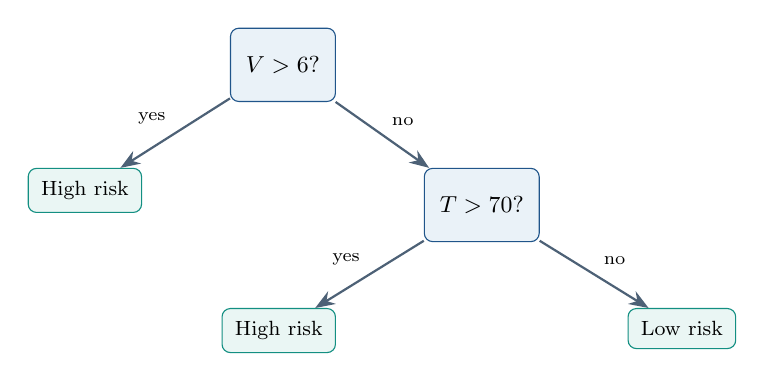
\begin{tikzpicture}[node distance=9mm and 12mm,scale=.93,transform shape]
\node[flow] (root) {$V>6$?};
\node[yesbox,below left=of root] (high1) {High risk};
\node[flow,below right=of root] (temp) {$T>70$?};
\node[yesbox,below left=of temp] (high2) {High risk};
\node[yesbox,below right=of temp] (low) {Low risk};
\draw[arr] (root) -- node[above left,font=\scriptsize]{yes} (high1);
\draw[arr] (root) -- node[above right,font=\scriptsize]{no} (temp);
\draw[arr] (temp) -- node[above left,font=\scriptsize]{yes} (high2);
\draw[arr] (temp) -- node[above right,font=\scriptsize]{no} (low);
\end{tikzpicture}
\hfill
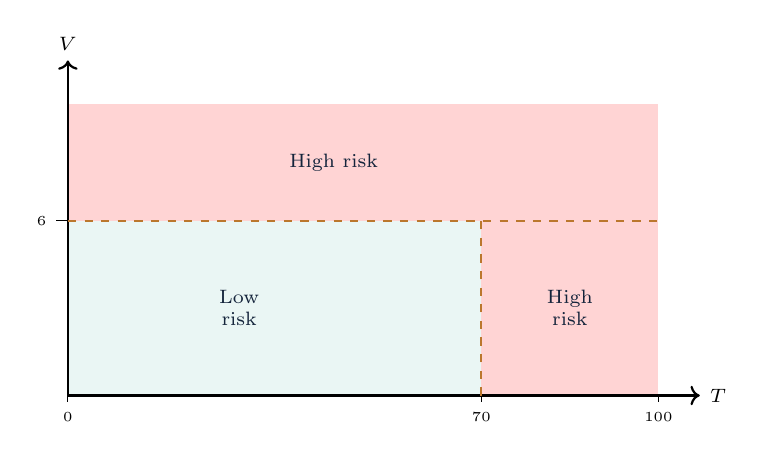
\begin{tikzpicture}[x=.075cm,y=.37cm,baseline=(current bounding box.center)]
\fill[palerteal] (0,0) rectangle (100,10);
\fill[red!17] (0,6) rectangle (100,10);
\fill[red!17] (70,0) rectangle (100,6);
\draw[->,thick] (0,0)--(107,0) node[right,font=\scriptsize] {$T$};
\draw[->,thick] (0,0)--(0,11.5) node[above,font=\scriptsize] {$V$};
\draw[dashed,amber,thick] (0,6)--(100,6);
\draw[dashed,amber,thick] (70,0)--(70,6);
\foreach \x in {0,70,100}{\draw (\x,0)--(\x,-.24) node[below,font=\tiny]{\x};}
\draw (0,6)--(-2,6) node[left,font=\tiny]{6};
\node[font=\scriptsize,align=center,text=navy] at (29,3) {Low\\risk};
\node[font=\scriptsize,align=center,text=navy] at (85,3) {High\\risk};
\node[font=\scriptsize,text=navy] at (45,8) {High risk};
\end{tikzpicture}
\caption{The same decision tree as a rule hierarchy (top) and a feature-space partition (bottom).
Every rectangular leaf region corresponds to one terminal prediction.}
\label{fig:tree_regions}
\end{figure}

A conventional \term{axis-aligned} tree splits on one feature at a time, $x_j\leq\theta_{\text{threshold}}$ versus $x_j>\theta_{\text{threshold}}$.
Its leaves divide feature space into $N_{\text{leaves}}$ disjoint regions.
A standard constant-leaf regression tree is
\begin{equation}
\boxed{
\hat f(x)
=
\sum_{j=1}^{N_{\text{leaves}}}
\underbrace{\theta_{\text{leaf},j}}_{\text{constant prediction in leaf }j}
\mathbb 1[x\in R_j]
}.
\end{equation}
Under squared-error loss, each $\theta_{\text{leaf},j}$ is usually the mean training target of the observations routed to that leaf.
A classification leaf can return the most frequent class or a vector of empirical class proportions.
Small-leaf proportions are not necessarily calibrated probabilities.
A tree therefore models a \emph{piecewise-constant function}, with conditional feature interactions created by its hierarchy: in \cref{fig:tree_regions}, temperature matters only for the branch with $V\leq6$.

\subsection{Learning a split}
\label{subsec:trees-learning-a-split}
At a node, a greedy learner generates allowable feature--threshold candidates, measures the reduction in a node criterion, selects the candidate with greatest gain, then recursively repeats on its children until a stopping rule applies.
The training process is a sequence of discrete structural decisions, rather than ordinary gradient descent through split thresholds.

\begin{figure}[htbp]\centering
\resizebox{\linewidth}{!}{%
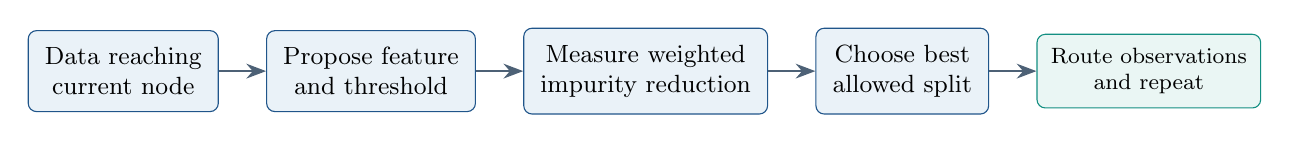
\begin{tikzpicture}[node distance=6mm and 6mm]
\node[flow] (data) {Data reaching\\current node};
\node[flow,right=of data] (search) {Propose feature\\and threshold};
\node[flow,right=of search] (score) {Measure weighted\\impurity reduction};
\node[flow,right=of score] (pick) {Choose best\\allowed split};
\node[yesbox,right=of pick] (recur) {Route observations\\and repeat};
\draw[arr] (data)--(search);\draw[arr] (search)--(score);\draw[arr] (score)--(pick);\draw[arr] (pick)--(recur);
\end{tikzpicture}}
\caption{Recursive tree fitting: a local split is chosen before the resulting subproblems are solved.
A stopping rule instead produces a leaf prediction.}
\label{fig:tree_fit_flow}
\end{figure}

For $N_{\text{classes}}$ classes, a common impurity is \term{Gini impurity}, $G=1-\sum_{j=1}^{N_{\text{classes}}}p_{\text{class }j}^{2}$.
Gini is zero in a pure node; in balanced binary classification it is $0.5$.
Suppose eight examples have four positives and four negatives, so $G_{\rm parent}=0.5$.
A candidate split creates a five-sample child with class counts $(4,1)$ and a three-sample pure child.
The five-sample impurity is $1-(4/5)^2-(1/5)^2=0.32$, giving
\begin{equation}
\boxed{\Delta G=0.5-\left(\frac58\,0.32+\frac38\,0\right)=0.30.}
\end{equation}
A split is useful because it creates more concentrated class distributions.
\emph{Entropy} $-\sum_j p_{\text{class }j}\log p_{\text{class }j}$ is another classification criterion.
Regression trees usually select splits that reduce within-node squared error/variance, or another specified regression objective; MAE-based methods naturally use median leaf predictions.
These are alternative definitions of \emph{good partition}, not unrelated model families.
See the loss-function discussion in \cref{sec:objectives-supervised-losses-for-continuous-targets,sec:objectives-classification-losses-and-logits}.

\begin{calloutintuition}
A tree learns a conditional partition of feature space.
Standard leaves output constants; complex global predictions arise by routing inputs to different local regions.
\end{calloutintuition}

\section{Tree structure, greedy search and regularisation}
\label{sec:trees-tree-structure-greedy-search-and-regularisation}
\subsection{Greedy splits need not find the best tree}
\label{subsec:trees-greedy-splits-need-not-find-the-best-tree}
Local optimisation can miss feature interactions.
For balanced XOR data, $y=x_1\oplus x_2$, each binary input feature alone leaves a 50--50 class mixture in both children.
The first split achieves zero Gini gain, even though a depth-two tree can represent XOR exactly after splitting on both features.
A greedy implementation that insists on positive immediate gain may never find it.
This separates \emph{representational capacity} from \emph{optimisation ability}.

\begin{figure}[htbp]\centering
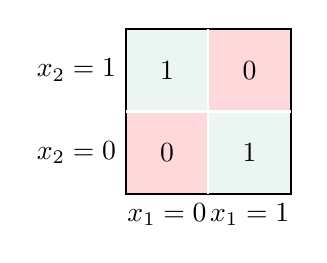
\begin{tikzpicture}[x=1.05cm,y=1.05cm]
\fill[red!15] (0,0) rectangle (1,1);\fill[palerteal] (1,0) rectangle (2,1);
\fill[palerteal] (0,1) rectangle (1,2);\fill[red!15] (1,1) rectangle (2,2);
\draw[thick] (0,0) rectangle (2,2);\draw[white,thick] (1,0)--(1,2) (0,1)--(2,1);
\node at (.5,.5){$0$};\node at (1.5,.5){$1$};\node at (.5,1.5){$1$};\node at (1.5,1.5){$0$};
\node[below] at (.5,0){$x_1=0$};\node[below] at (1.5,0){$x_1=1$};
\node[left] at (0,.5){$x_2=0$};\node[left] at (0,1.5){$x_2=1$};
\end{tikzpicture}
\caption{Balanced XOR: neither first-level split helps on its own, but two levels perfectly separate the classes.}
\label{fig:tree_xor}
\end{figure}

\subsection{Depth, leaves and pruning}
\label{subsec:trees-depth-leaves-and-pruning}
A binary tree with maximum depth $N_{\text{depth}}$ has at most $2^{N_{\text{depth}}}$ leaves; depth 1 is a \emph{decision stump}.
More leaves can approximate increasingly local structure, but individual leaf estimates may rely on few observations.
This is the bias--variance trade-off already introduced in \cref{sec:evaluation-overfitting-underfitting-and-the-bias-variance-tradeoff}.

\begin{center}\small
\begin{tabularx}{\linewidth}{@{}L{.24\linewidth}YY@{}}\toprule
Control & What it constrains & Trade-off\\\midrule
Maximum depth & Number of sequential decisions & Less depth limits interactions; greater depth can fit noise\\
Minimum samples per leaf & Evidence supporting each local estimate & Larger leaves stabilise predictions but smooth local structure\\
Minimum samples to split & Eligibility to expand a node & Earlier stopping versus finer partitions\\
Maximum leaf count & Number of distinct terminal regions & Direct budget for partition complexity\\
Minimum split improvement & Gain required to add a split & Reject weak gains, possibly including useful precursors\\
Pruning strength & Number of retained branches after growing & Simpler tree versus potentially discarded genuine structure\\\bottomrule
\end{tabularx}
\end{center}

\term{Pre-pruning} prevents a split when a limit is reached; \term{post-pruning} removes branches from a larger fitted tree.
Cost-complexity pruning makes the trade-off explicit:
\begin{equation}
\underbrace{J(T)}_{\text{selection objective}}
=
\underbrace{L_{\mathrm{train}}(T)}_{\text{fit}}
+
\underbrace{\alpha N_{\text{leaves}}(T)}_{\text{complexity cost}}.
\end{equation}
Each extra leaf must therefore buy enough training improvement to justify its penalty.
Pruning is not a complete solution to greedy-search errors: it simplifies already-discovered structures, rather than exploring every possible tree.

\subsection{Growth strategy and split geometry}
\label{subsec:trees-growth-strategy-and-split-geometry}
\term{Level-wise} growth expands eligible nodes layer by layer.
\term{Best-first/leaf-wise} growth expands the current leaf promising the greatest loss reduction.
Leaf-wise growth concentrates complexity in difficult regions but can create deep low-support paths; level-wise growth allocates depth more evenly.
Level-wise does \emph{not} imply symmetric splitting: nodes at the same depth can still use different tests.

An axis-aligned split tests one feature, such as $x_j>\theta_{\text{threshold}}$; an \term{oblique split} tests $\theta_{\text{split}}^\top x>\theta_{\text{threshold}}$.
A diagonal boundary, such as $T+2V>80$, may require many staircase-like axis-aligned regions but only one oblique split.
Oblique splits increase geometric expressivity and typically make split search harder.

\begin{calloutbias}
If the target is well described by hierarchical single-feature thresholds and locally constant regions, standard trees represent the structure efficiently.
If the boundary is smooth or strongly rotated, they may need many leaves; deeper trees add expressivity while increasing estimation variance.
\end{calloutbias}
Depth and leaf support are related but distinct controls.
\begin{calloutmemoryhook}
Depth limits interaction length; minimum leaf size limits evidence per local prediction.
\end{calloutmemoryhook}

\section{Bagging, Random Forests and ExtraTrees}
\label{sec:trees-bagging-random-forests-and-extratrees}
A single tree can be unstable: removing or changing a few observations may change a high-level split and many downstream predictions.
\term{Bagging} (bootstrap aggregating) reduces this variation by fitting multiple trees to bootstrap samples and aggregating their outputs.

\begin{figure}[htbp]\centering
\resizebox{.9\linewidth}{!}{%
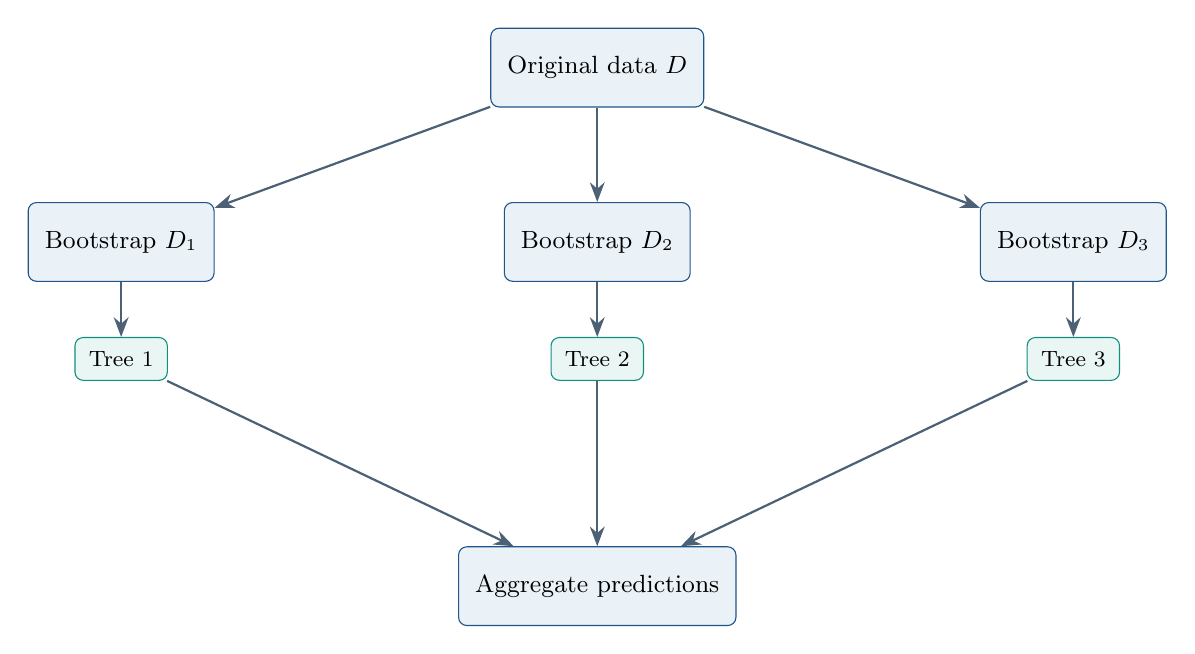
\begin{tikzpicture}[node distance=7mm and 13mm]
\node[flow] (d) {Original data $D$};
\node[flow,below left=12mm and 35mm of d] (s1) {Bootstrap $D_1$};
\node[flow,below=12mm of d] (s2) {Bootstrap $D_2$};
\node[flow,below right=12mm and 35mm of d] (s3) {Bootstrap $D_3$};
\node[yesbox,below=of s1] (t1) {Tree 1};
\node[yesbox,below=of s2] (t2) {Tree 2};
\node[yesbox,below=of s3] (t3) {Tree 3};
\node[flow,below=21mm of t2] (agg) {Aggregate predictions};
\foreach \s in {s1,s2,s3}{\draw[arr] (d)--(\s);}
\foreach \i in {1,2,3}{\draw[arr] (s\i)--(t\i);\draw[arr] (t\i)--(agg);}
\end{tikzpicture}}
\caption{Bagging: independent bootstrap-fitted trees are combined at prediction time.
Individual fits can be trained in parallel.}
\label{fig:tree_bagging}
\end{figure}

Each bootstrap sample draws $N_{\text{examples}}$ observations \emph{with replacement} from $N_{\text{examples}}$ originals.
For large $N_{\text{examples}}$, about $63.2\%$ of originals appear at least once and about $36.8\%$ are out-of-bag for that tree.
Averaging regression predictions or class probabilities reduces variation when the trees' errors are not perfectly correlated.
Majority voting is another classification aggregation rule.

For $N_{\text{trees}}$ trees with common prediction variance $\sigma^2$ and pairwise correlation $\rho$, the equal-correlation model gives
\begin{equation}
\boxed{
\Var(\bar f)
=
\underbrace{
\underbrace{\sigma^2}_{\text{single-tree variance}}
\underbrace{\rho}_{\text{pairwise error correlation}}
}_{\text{shared variance: averaging cannot remove}}
+
\underbrace{
\sigma^2\frac{1-\rho}{N_{\text{trees}}}
}_{\text{unshared variance: shrinks with more trees}}
}.
\end{equation}
More trees only reduce the unshared component; decorrelation is therefore as important as tree count.
This is a simplified equal-variance/equal-correlation model, not a universal forest error law; connect it to the broader bias--variance picture in \cref{sec:evaluation-overfitting-underfitting-and-the-bias-variance-tradeoff}.

\term{Random Forests} add random selection of eligible features \emph{at each split}, commonly together with bootstrapping.
This decorrelates trees that might otherwise make the same dominant early choices.
Too much randomisation weakens individual trees, so diversity and individual predictive quality trade off.
\term{ExtraTrees} also randomise candidate thresholds and often use the original sample rather than bootstrapping by default.
The extra randomness can improve diversity and split-search efficiency while increasing individual-tree bias.

\begin{center}\small
\begin{tabularx}{\linewidth}{@{}L{.20\linewidth}YY@{}}\toprule
Method & Randomness & Primary idea\\\midrule
Bagged trees & Resample training rows & Average unstable learners\\
Random Forest & Resample rows; random features per node & Reduce correlation between learners\\
ExtraTrees & Random candidate thresholds; often random features & Additional split diversity, often less split-search work\\\bottomrule
\end{tabularx}
\end{center}

\term{Out-of-bag (OOB) evaluation} predicts each training observation using only trees whose bootstrap samples omitted it.
It offers an internal performance estimate under suitable sampling assumptions, but does not fix temporal or grouped leakage (\cref{sec:evaluation-cross-validation-and-fold-choice,sec:evaluation-model-selection-and-data-leakage}).

\begin{calloutmemoryhook}
Random Forests win by averaging diversity; more trees cannot remove shared error.
\end{calloutmemoryhook}

\section{Boosting: learning successive corrections}
\label{sec:trees-boosting-learning-successive-corrections}
Where bagging trains diverse trees independently, \term{boosting} trains a sequence of weak or limited-complexity learners that collectively improve a predictor.
\term{AdaBoost} reweights training examples according to previous classification errors; hard examples gain relative emphasis.
This can be useful, but mislabeled examples are also hard and may attract excessive attention.

\subsection{Gradient boosting as functional optimisation}
\label{subsec:trees-gradient-boosting-as-functional-optimisation}
\term{Gradient boosting} updates the current predictor by adding a new correction tree:
\begin{equation}
\boxed{
\underbrace{F_t(x)}_{\text{updated ensemble}}
=
\underbrace{F_{t-1}(x)}_{\text{current ensemble}}
+
\underbrace{\eta}_{\text{shrinkage}}
\underbrace{h_t(x)}_{\text{new correction tree}}
}.
\end{equation}
Each stage improves the current ensemble rather than refitting the original target from scratch.

For squared-error regression, suppose the current model predicts $5$ for targets $(3,5,7)$.
The residuals are $(-2,0,2)$.
If a correction tree fits these residuals exactly and $\eta=0.5$, the updated predictions become $(4,5,6)$.
The ensemble improves through a series of moderate adjustments.

More generally, each training example supplies the prediction-space direction
\begin{equation}
\boxed{
\underbrace{r_{i,t}}_{\text{pseudo-residual}}
=
-\left.\underbrace{\frac{\partial L(y_i,F)}{\partial F}}_{\text{loss slope in prediction space}}\right|_{F=F_{t-1}(x_i)}
}.
\end{equation}
A tree approximates this direction as a function of inputs; its terminal output values may subsequently be optimised for the specified loss.
Squared-error pseudo-residuals are ordinary residuals (up to loss convention).
For binary logistic loss differentiated with respect to logits, the negative gradient is label minus predicted probability.
This connects tree boosting to loss design in \cref{sec:objectives-supervised-losses-for-continuous-targets,sec:objectives-classification-losses-and-logits}.

\begin{figure}[htbp]\centering
\resizebox{\linewidth}{!}{%
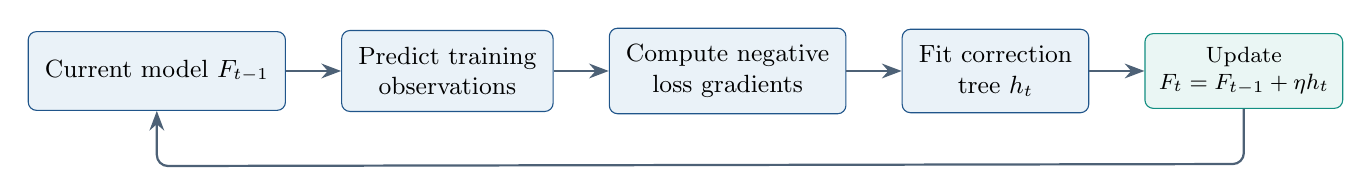
\begin{tikzpicture}[node distance=6mm and 7mm]
\node[flow] (f) {Current model $F_{t-1}$};
\node[flow,right=of f] (p) {Predict training\\observations};
\node[flow,right=of p] (g) {Compute negative\\loss gradients};
\node[flow,right=of g] (t) {Fit correction\\tree $h_t$};
\node[yesbox,right=of t] (u) {Update\\$F_t=F_{t-1}+\eta h_t$};
\draw[arr] (f)--(p);\draw[arr] (p)--(g);\draw[arr] (g)--(t);\draw[arr] (t)--(u);
\draw[arr,rounded corners] (u.south)--++(0,-.7)--([yshift=-.7cm]f.south)--(f.south);
\end{tikzpicture}}
\caption{Gradient boosting is stage-wise optimisation in prediction-function space: fit a correction, add it, recompute the next direction.}
\label{fig:tree_boost_flow}
\end{figure}

This is related to gradient descent but not identical to backpropagating through a fixed neural network.
Neural-network training typically updates continuously parameterised weights within an existing architecture.
Boosting adds a \emph{new fitted function} at each iteration; hard tree split decisions are not usually differentiated end to end.
The SGD and adaptive-optimiser discussion in \cref{sec:optimisation-batch-gradient-descent-vs-sgd-vs-mini-batch-sgd,sec:optimisation-adam-momentum-plus-adaptive-step-sizes} concerns a different parameterisation of the optimisation problem.


\subsection{Ranking-aware boosting: LambdaMART}
\label{subsec:trees-lambdamart}
A ranking metric such as NDCG changes only when item order changes, so it is awkward as a direct smooth training loss (\cref{sec:objectives-ranking-and-preference-objectives,sec:evaluation-retrieval-and-ranking-metrics}).
LambdaRank-style training instead creates pairwise correction signals and weights them by the ranking consequence of swapping the pair.
If reversing two items would greatly change NDCG, that ordering error receives a stronger update than a swap deep in the list with almost no metric effect.

\begin{figure}[htbp]
\centering
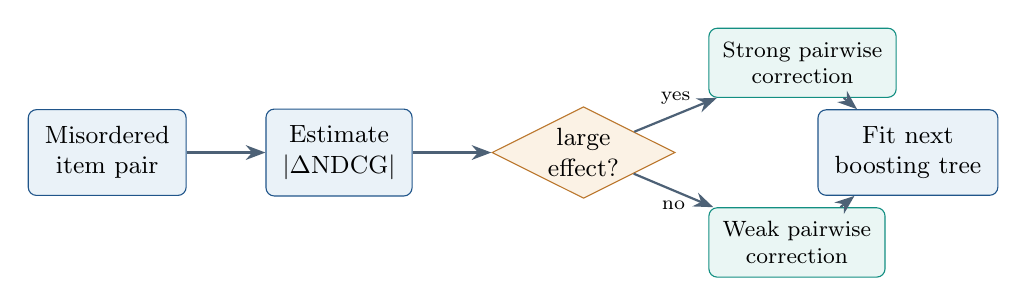
\begin{tikzpicture}[node distance=8mm and 10mm]
\node[flow] (pair) {Misordered\\item pair};
\node[flow,right=of pair] (delta) {Estimate\\$|\Delta\mathrm{NDCG}|$};
\node[decisionnode,right=of delta] (big) {large\\effect?};
\node[yesbox,above right=4mm and 10mm of big] (strong) {Strong pairwise\\correction};
\node[yesbox,below right=4mm and 10mm of big] (weak) {Weak pairwise\\correction};
\node[flow,right=18mm of big] (tree) {Fit next\\boosting tree};
\draw[arr] (pair)--(delta);
\draw[arr] (delta)--(big);
\draw[arr] (big)--node[above,font=\scriptsize]{yes}(strong);
\draw[arr] (big)--node[below,font=\scriptsize]{no}(weak);
\draw[arr] (strong)--(tree);
\draw[arr] (weak)--(tree);
\end{tikzpicture}
\caption{LambdaMART keeps the stage-wise tree-boosting mechanism but makes the correction signal sensitive to where a ranking mistake occurs.}
\end{figure}

LambdaMART combines these ranking-aware ``lambda'' updates with MART-style gradient-boosted regression trees.
The important conceptual change is not a new tree primitive: it is a new objective signal layered onto the boosting machinery already developed above.

\begin{calloutmemoryhook}
LambdaMART is boosting where high-impact ranking mistakes get stronger correction signals.
\end{calloutmemoryhook}

\subsection{Curvature and second-order updates}
\label{subsec:trees-curvature-and-second-order-updates}
Second-order tree boosting also uses curvature of the loss with respect to the current prediction.
For one constant-output leaf, a common local quadratic update is
\begin{equation}
\boxed{
\underbrace{\theta_{\text{leaf update}}}_{\text{constant correction in this leaf}}
=
-\frac{
\underbrace{\sum_{i\in\mathrm{leaf}}\frac{\partial L_i}{\partial F_i}}_{\text{accumulated loss slope}}
}{
\underbrace{\sum_{i\in\mathrm{leaf}}\frac{\partial^2L_i}{\partial F_i^2}}_{\text{prediction-space curvature}}
+
\underbrace{\lambda_{\text{leaf}}}_{\text{shrink large leaf updates}}
}
}.
\end{equation}
This is scalar curvature in prediction space, not the full parameter Hessian; compare \cref{subsec:la-hessian,sec:optimisation-newton-s-method-and-other-second-order-methods}.

\subsection{Learning rate, depth and early stopping}
\label{subsec:trees-learning-rate-depth-and-early-stopping}
Smaller $\eta$ gives more conservative corrections, normally requiring more boosting stages.
Large $\eta$ can fit quickly but may overstep or fit noise.
The \emph{learning rate and number of trees must be tuned together}; doubling tree count does not exactly undo halving $\eta$, because the intermediate ensemble and all subsequent correction targets change.

A depth-one stump contributes a function of one feature; an additive ensemble of such stumps cannot represent genuine cross-feature interactions on its raw score scale without richer components.
Depth-two and deeper trees can encode conditional interactions within each stage.
Validation-based early stopping selects the iteration before continuing improvement on the training loss ceases to help generalisation (\cref{sec:stability-early-stopping-stop-before-the-model-overfits,sec:evaluation-model-selection-and-data-leakage}).

\begin{center}\small
\begin{tabularx}{\linewidth}{@{}L{.25\linewidth}YY@{}}\toprule
Design & Bagging / Random Forest & Gradient boosting\\\midrule
Tree dependence & Trees independently fitted & Each stage depends on preceding model\\
Combination & Average or vote & Add weighted corrections\\
Main benefit & Stabilise high-variance predictors & Build fit through stage-wise loss reduction\\
Typical trees & Often deep & Often shallow or leaf-limited\\
Parallelism & Trees can be trained concurrently & Boosting stages are sequential\\
Important controls & Tree count, randomness, leaf size & Learning rate, stages, leaf size, regularisation\\\bottomrule
\end{tabularx}
\end{center}

\begin{calloutpractical}
For gradient boosting, monitor validation loss across rounds and use early stopping.
A falling training loss does not prove the next tree improves deployment performance.
\end{calloutpractical}

\section{XGBoost, LightGBM and CatBoost: what changed?}
\label{sec:trees-xgboost-lightgbm-and-catboost-what-changed}
The historical progression is best seen as multiple related developments rather than one mandatory chain.
The useful story is the accumulation of problems and fixes, not a claim that each method replaced the previous one.

\begin{center}
\small
\begin{tabularx}{\linewidth}{@{}L{.16\linewidth}L{.22\linewidth}YY@{}}
\toprule
\textbf{Step} & \textbf{What changed} & \textbf{Why it was added} & \textbf{Consequence / new trade-off} \\
\midrule
CART & Recursive threshold partitioning & Represent nonlinear conditional rules & Flexible but unstable single trees \\
Bagging / Random Forest & Average diversified trees & Reduce variance from unstable fits & More compute; averaging cannot remove shared error \\
AdaBoost / Gradient Boosting & Add learners sequentially & Correct current mistakes or descend a loss & Strong staged fit; stages become dependent \\
XGBoost & Second-order updates, explicit penalties, scalable split search & Regularise and accelerate boosting & More design knobs and systems complexity \\
LightGBM / CatBoost & Selective computation, categorical handling, constrained growth choices & Improve efficiency or data handling & Extra approximation and inductive-bias choices \\
\bottomrule
\end{tabularx}
\end{center}

The modern libraries below share a core boosting framework but emphasise different implementation choices.

\subsection{XGBoost: explicit regularisation and efficient optimisation}
\label{subsec:trees-xgboost-explicit-regularisation-and-efficient-optimisation}
XGBoost popularised a scalable second-order tree-boosting system with explicit structural penalties.
A representative objective separates predictive fit from structural/leaf penalties:
\begin{equation}
\underbrace{\sum_i L(y_i,F(x_i))}_{\text{predictive loss}}
+
\sum_{t=1}^{N_{\text{trees}}}
\left(
\underbrace{\gamma N_{\text{leaves},t}}_{\text{cost of adding leaves}}
+
\underbrace{
\frac{\lambda}{2}
\sum_{j=1}^{N_{\text{leaves},t}}\theta_{\text{leaf},t,j}^{2}
}_{\text{shrink large leaf outputs}}
\right).
\end{equation}
The two penalties regulate structural complexity and correction magnitude separately.
This is regularisation of tree structure/leaf outputs rather than a generic neural-network weight penalty; compare \cref{sec:stability-regularisation-l1-and-l2}.
Other design choices include row/column subsampling, missing-value-aware routing, approximate or histogram split search, and efficient memory/parallel processing.
Leaf-count penalties and leaf-weight shrinkage regulate different forms of complexity.

\subsection{Histogram split search}
\label{subsec:trees-histogram-split-search}
Searching every distinct numerical threshold can be expensive.
A histogram learner maps numerical values to a finite set of bins, accumulates gradient/curvature statistics within each bin, and searches boundaries between bins.
For example, $(1.1,1.2,1.5,2.8,3.0,3.1,4.9,5.0)$ may be quantised into three bins containing $(1.1,1.2,1.5)$, $(2.8,3.0,3.1)$ and $(4.9,5.0)$.

This reduces split-search and memory cost at the expense of threshold resolution.
The approximation need not worsen validation performance, but its quality and runtime depend on bin count and the distribution of feature values.
Histogram methods now appear in several GBDT libraries; they are not unique to LightGBM.

\subsection{LightGBM: selective use of computation}
\label{subsec:trees-lightgbm-selective-use-of-computation}
LightGBM is associated with several efficiency choices:
\begin{itemize}
\item \term{Leaf-wise growth}: preferentially expand the leaf with greatest gain; efficient use of a leaf budget, but potentially deep low-support branches.
\item \term{GOSS (Gradient-based One-Side Sampling)}: keep high-gradient observations, sample some low-gradient observations, then reweight as appropriate for split-gain estimation.
This saves work while retaining influential gradient information; it is an available sampling strategy, not necessarily enabled in every configuration.
\item \term{EFB (Exclusive Feature Bundling)}: bundle sparse features that are mutually or nearly mutually exclusive, reducing effective dimensionality.
Exclusivity means seldom nonzero together, not merely low correlation.
\item \term{Histogram-based processing}: quantise features and aggregate split statistics, reducing work relative to exhaustive threshold scans.
\end{itemize}
The common principle is to allocate compute to observations, features and regions where it is likely to matter.
These approximations can alter accuracy and regularisation, and must be tested under equal resource budgets.

\subsection{CatBoost: ordered categories and symmetric trees}
\label{subsec:trees-catboost-ordered-categories-and-symmetric-trees}
Categorical features create a representation problem.
One-hot encoding can greatly expand high-cardinality features.
Global target encoding compresses them by replacing each category with a target statistic, but can leak an observation's own label into its input.
For a category represented by one example, naive full-training target encoding can directly expose the answer.

CatBoost uses \term{ordered categorical statistics}: conceptually, an example's category statistic depends on earlier observations in a chosen ordering, not on its own target, together with smoothing and other implementation details.
\term{Ordered boosting} is a distinct, related training procedure designed to reduce prediction shift arising from reused target information in gradient estimation.
Neither idea removes the need for appropriate temporal and group validation; a random permutation is not a replacement for chronology.

CatBoost also characteristically uses \term{symmetric (oblivious) trees}, where all nodes at the same depth use the same test.
This constrains the hypothesis class and supports efficient routing.
Unlike merely \emph{level-wise} trees, symmetric trees cannot choose separate splits at different nodes of one level.
CatBoost also offers other growth policies.

\begin{center}\footnotesize
\begin{tabularx}{\linewidth}{@{}L{.17\linewidth}YYY@{}}\toprule
 & XGBoost & LightGBM & CatBoost\\\midrule
Emphasis & Scalable regularised boosting & Efficiency and selective allocation & Categories, prediction shift, symmetric trees\\
Split search & Exact/approximate/histogram options & Histogram-based & Quantised feature processing\\
Growth & Depth-wise or loss-guided variants & Leaf-wise characteristically & Symmetric by default, alternatives\\
Categories & Native handling or external encoding & Native handling or encoding & Ordered statistics and other transforms\\
Characteristic ideas & Second-order updates, sparse-aware handling, explicit penalties & GOSS, EFB, histogram subtraction & Ordered boosting, ordered category statistics\\\bottomrule
\end{tabularx}
\end{center}

\begin{calloutpractical}
Library names are not independent hypotheses: compare specific growth, categorical-handling, sampling and regularisation mechanisms under a fair validation and compute budget.
\end{calloutpractical}

\section{Research optionality: what can be changed?}
\label{sec:trees-research-optionality-what-can-be-changed}
A tree system has several distinct design layers: input representation, base-tree structure, ensemble mechanism, optimisation objective, sampling procedure and computational implementation.
Different modifications target different limitations.

\small
\begin{longtable}{@{}L{.21\linewidth}L{.35\linewidth}L{.35\linewidth}@{}}
\caption{Degrees of experimentation for tree-based methods.}\label{tab:tree_research_axes}\\
\toprule Design axis & Representative alternatives & Mechanism to measure\\\midrule\endfirsthead
\toprule Design axis & Representative alternatives & Mechanism to measure\\\midrule\endhead
Split geometry & Axis-aligned versus oblique & Fit to rotated boundaries; split count; compute\\
Split search & Greedy versus lookahead & Discover interactions with initially weak splits\\
Leaf outputs & Constant versus linear local models & Approximation of smooth local behaviour\\
Growth policy & Level-wise versus best-first & Leaf depths, support and loss reduction\\
Ensemble & Single tree, bagging, boosting & Stability versus progressive loss reduction\\
Loss & Squared, robust, logistic, quantile & Alignment to task and error costs\\
Sampling & Bootstrap, feature subsets, gradient-aware & Prediction correlation, training cost and variance\\
Regularisation & Pruning, leaf penalties, shrinkage & Complexity, noisy-fit sensitivity\\
Categories & One-hot, ordered statistics, native splits & High-cardinality generalisation and leakage\\
Split resolution & Exact values versus histogram bins & Speed--accuracy--memory trade-off\\
Uncertainty & Point, quantile, distributional predictions & Calibration and coverage under assumptions\\
\bottomrule\end{longtable}
\normalsize

A research improvement can come from a richer \emph{hypothesis class} (oblique splits or linear leaves), better \emph{optimisation} (lookahead or second-order updates), better \emph{regularisation} (leaf penalties or shrinkage), better \emph{representation} (categorical statistics), or better \emph{systems engineering} (histograms and memory layout).
These are different causal explanations of performance gains.

Three useful controlled experiments are: compare bagging with Random Forests while logging tree correlation and ensemble error; compare level-wise with leaf-wise growth under a matched leaf budget while measuring leaf support and depth; and compare first- with second-order boosting using matched objectives while reporting wall-clock cost \emph{as well as} improvement per round.

\begin{calloutdegreeofexperiment}
Vary split geometry/search, growth policy, leaf model, ensemble type, objective, row/feature sampling, regularisation, category handling, histogram resolution, uncertainty output, and compute budget.
\end{calloutdegreeofexperiment}

\section{Inductive bias and model selection}
\label{sec:trees-inductive-bias-and-model-selection}
A tree's built-in preferences are: useful single-feature thresholds, hierarchical interactions, locally constant predictions, and adaptive refinement of regions.
These assumptions can help with heterogeneous tabular features and abrupt conditional effects.
They can be inefficient for oblique boundaries, smooth globally varying functions and behaviour far outside the training support (\cref{sec:nfl-inductive-bias-the-assumptions-that-make-learning-possible}).

\subsection{Extrapolation and feature transformations}
\label{subsec:trees-extrapolation-and-feature-transformations}
Suppose the physical target is $y=2x$ and training data only cover $0\leq x\leq10$.
A linear model may extrapolate the same slope to $x=15$.
A standard regression tree routes every sufficiently large $x$ to its terminal rightmost leaf and returns its constant estimate.
A finite sum or average of such trees likewise stays constant beyond all its final thresholds along that coordinate, holding other features fixed.
More trees improve within-support resolution but do not automatically recover the outside-support physical law.

\begin{figure}[htbp]\centering
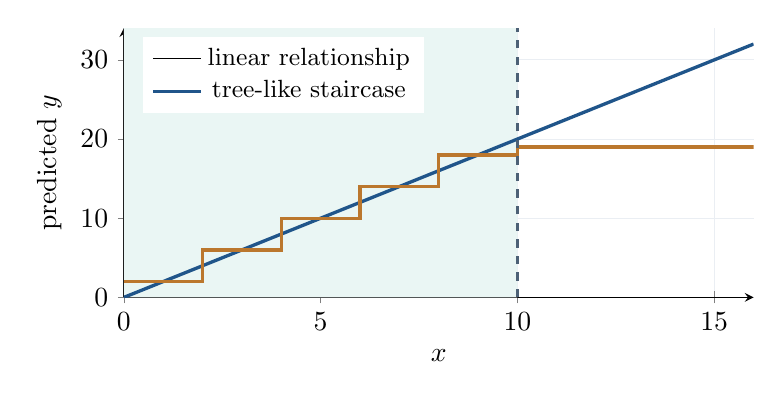
\begin{tikzpicture}
\begin{axis}[width=.79\linewidth,height=5.0cm,xmin=0,xmax=16,ymin=0,ymax=34,axis lines=left,xlabel={$x$},ylabel={predicted $y$},xtick={0,5,10,15},ytick={0,10,20,30},grid=both,grid style={rulegray!50},legend style={at={(.03,.97)},anchor=north west,font=\small,draw=none,fill=white}]
\addplot[draw=none,fill=palerteal] coordinates {(0,0)(10,0)(10,34)(0,34)} \closedcycle;
\addplot[very thick,deepblue,domain=0:16] {2*x};\addlegendentry{linear relationship}
\addplot[very thick,amber,const plot] coordinates {(0,2)(2,6)(4,10)(6,14)(8,18)(10,19)(16,19)};\addlegendentry{tree-like staircase}
\addplot[dashed,slate,thick] coordinates {(10,0)(10,34)};
\end{axis}
\end{tikzpicture}
\caption{Schematic extrapolation: a constant-leaf tree saturates once an input lies beyond the last training-supported split; a linear function can continue its slope.
Curves are illustrative, not fitted experimental results.}
\label{fig:tree_extrapolation}
\end{figure}

Because exact axis-aligned splits primarily depend on feature ordering, strictly monotonic transforms of a numerical feature preserve the representable partitions (after transforming thresholds), unlike a general rotation that mixes features.
Practical fitted models may still change owing to histogram binning, ties and numerical detail.
Standard scaling is often unnecessary for exact tree splits; it may still matter for models or preprocessing stages around the tree (\cref{sec:representation-scaling-standardisation-and-leakage}).

\begin{calloutpractical}
Known physical law plus unexplained residuals: investigate $\hat y(x)=f_{\mathrm{physics}}(x)+f_{\mathrm{trees}}(x)$.
The physical term can encode extrapolative structure; the learned correction still needs out-of-domain validation.
\end{calloutpractical}

\begin{center}\small
\begin{tabularx}{\linewidth}{@{}L{.22\linewidth}YY@{}}\toprule
Model family & Preferred structure & Notable limitation to test\\\midrule
Linear / additive model & Global linear or additive effects & Missing interactions and discontinuities\\
Single tree & Hierarchical threshold rules & Instability; staircase approximation\\
Random Forest & Average diverse local partitions & Correlated errors; extrapolation\\
Boosted trees & Sequential additive partition corrections & Overfit to residual noise; extrapolation\\
Neural network & Learned continuous representations & Data/optimisation and architectural bias\\
Physics-informed/hybrid & Governing laws plus fitted deviations & Error from incorrect scientific assumptions\\\bottomrule
\end{tabularx}
\end{center}

\section{Evaluation, explanation and failure modes}
\label{sec:trees-evaluation-explanation-and-failure-modes}
\subsection{Evaluate the deployment task, not a random row split}
\label{subsec:trees-evaluate-the-deployment-task-not-a-random-row-split}
In longitudinal data, measurements from one machine or person can be strongly dependent.
Randomly dividing rows may put the same entity in training and test sets.
For forecasting, training on later observations than those being tested can introduce future-information leakage.
Choose chronological and/or grouped validation according to the actual deployment question (\cref{sec:evaluation-cross-validation-and-fold-choice,sec:adaptation-domain-adaptation-the-data-distribution-changes}).

Supervised feature engineering is another leakage route.
Computing global category target means, performing label-dependent feature selection before splitting, or using a row's own label during its target encoding can all inflate apparent validation results.
Fit transformations within the training fold, with cross-fitting or ordered encodings when appropriate.
Missingness may itself be predictive, but changing collection practices can create shift; an integer category code should not silently become an ordinal physical quantity.

\subsection{Metrics, importance and causal interpretation}
\label{subsec:trees-metrics-importance-and-causal-interpretation}
Rare-event prediction should consider precision, recall and PR curves, not accuracy alone; log loss and calibration measure different properties from ranking AUC.
Operating thresholds should reflect false-alarm and missed-event costs.
See the worked definitions in \cref{sec:evaluation-precision-recall-and-f1,sec:evaluation-roc-curves-auc-roc-and-precision-recall,sec:evaluation-decision-thresholds}.

Three common explanations answer different questions:
\begin{itemize}
\item \term{Impurity importance} accumulates training-criterion reductions attributed to features; continuous/high-cardinality features can receive a structural advantage.
\item \term{Permutation importance} measures held-out performance deterioration when one feature is shuffled; correlated predictors can substitute for one another, masking individual importance.
\item \term{SHAP} assigns additive contributions to a prediction relative to a chosen reference/distributional convention; an attribution is not an intervention or an automatic causal effect.
\end{itemize}
Partial dependence averages predictions while changing a chosen feature; individual conditional expectation traces this for one observation.
With strongly dependent features, intervening on one coordinate while holding others unchanged can generate unrealistic feature combinations.
Such plots describe a fitted model, not necessarily the true data-generating mechanism.

\begin{center}\small
\begin{tabularx}{\linewidth}{@{}L{.27\linewidth}YY@{}}\toprule
Failure mode & Mechanism & Useful check\\\midrule
Overfitting & Tiny leaves; late boosting stages fit noise & Leaf limits, early stopping, held-out trends\\
Leakage & Targets or future/group information in features & Pipeline audit, grouped/time splits\\
Poor calibration & Predicted scores do not match event frequencies & Reliability curves; probability scores such as log loss or Brier score\\
Shift & Deployment population differs from training & Time/site holdouts; drift monitoring\\
Misleading importance & Correlated predictors or split-cardinality effects & Refit stability; grouped perturbations\\
Slow inference & Many trees, deep paths, expensive preprocessing & Profile end-to-end latency and memory\\
Extrapolation error & Terminal leaves return learned local values & Validate beyond training support; hybrid model\\\bottomrule
\end{tabularx}
\end{center}

\begin{calloutmemoryhook}
Feature attribution describes model dependence, not causal mechanism.
\end{calloutmemoryhook}

\section{Extensions and a complete research example}
\label{sec:trees-extensions-and-a-complete-research-example}
\subsection{Beyond standard trees}
\label{subsec:trees-beyond-standard-trees}
Conventional trees are not the end of the design space:
\begin{itemize}
\item \term{Differentiable trees} soften routing, for example $p_{\mathrm{right}}(x)=\sigma((\theta_{\text{split}}^\top x-\theta_{\text{threshold}})/\tau_{\text{routing softness}})$, enabling gradients through route probabilities.
Small $\tau_{\text{routing softness}}$ approaches hard routing but may cause saturated gradients; soft routing can also make inference costlier.
\item \term{Model trees} predict $\theta_{\text{leaf},j}^\top x+\theta_{\text{bias},j}$ inside region $R_j$ rather than a constant.
This fits smooth local effects more directly, but local parameter fitting and continuity across boundaries become design issues.
\item \term{Quantile or distributional boosting} targets uncertainty rather than only a conditional mean.
Conformal calibration can provide prediction sets when future cases behave like the calibration cases under the method's stated assumptions; coverage under shift still requires examination.
\item \term{Constrained trees} may enforce monotonic effects or limit interactions, adding domain-specific bias.
An incorrect constraint can create systematic error.
\item \term{Neural--tree hybrids and tabular foundation models} change representation learning or transfer information across tasks rather than only improving the split search of a newly fitted tree.
\end{itemize}

\subsection{Worked design: failure forecasting on repeated measurements}
\label{subsec:trees-worked-design-failure-forecasting-on-repeated-measurements}
Suppose 500 machines produce repeated sensor measurements over several years.
The inputs include numerical readings and categorical manufacturers; failures are rare; labels are noisy and inference must be fast.
A defensible workflow is:
\begin{enumerate}
\item Define the unit of prediction (next-month failure per machine) and the information actually available at decision time.
\item Use chronological validation, and hold out complete machines as well if the deployment goal includes unseen machines.
Repeated rows do not equal independent machines.
\item Fit a simple physical or parametric baseline, a regularised single tree, a Random Forest and a regularised GBDT; evaluate suitable categorical treatment without target leakage.
\item Compare minimum leaf size, tree complexity, boosting shrinkage and early stopping; report stability across machines, time windows and random seeds.
\item Evaluate PR behaviour, calibration and application-specific false-alarm costs, not accuracy in isolation.
\item Profile end-to-end inference latency and memory.
Investigate whether manufacturer effects and feature importances remain stable across valid holdouts.
\end{enumerate}
This experiment tests specific modelling assumptions as well as parameter values.
The appropriate ensemble cannot be inferred from its library name alone.

\begin{calloutmemoryhook}
Trees partition; bagging averages diverse partitions; boosting adds loss-driven corrections.
\end{calloutmemoryhook}

\section{Further reading}
\label{sec:trees-further-reading}
\begin{itemize}
\item Chen and Guestrin (2016), \href{https://arxiv.org/abs/1603.02754}{\emph{XGBoost: A Scalable Tree Boosting System}}: regularised boosting and scalable split search.
\item Ke et al. (2017), \href{https://papers.nips.cc/paper_files/paper/2017/hash/6449f44a102fde848669bdd9eb6b76fa-Abstract.html}{\emph{LightGBM: A Highly Efficient Gradient Boosting Decision Tree}}: GOSS and EFB.
\item Prokhorenkova et al. (2018), \href{https://arxiv.org/abs/1706.09516}{\emph{CatBoost: Unbiased Boosting with Categorical Features}}: ordered statistics and boosting.
\item Grinsztajn et al. (2022), \href{https://arxiv.org/abs/2207.08815}{\emph{Why Do Tree-Based Models Still Outperform Deep Learning on Typical Tabular Data?}}: comparative inductive-bias study with a limited benchmark scope.
\end{itemize}

\chapter{Architecture: CNNs}
\label{chap:cnn}
We have already introduced convolution's two core assumptions: useful patterns are local and that the same detector can be reused.
So, we will now extend that mental model into efficient vision systems, detection, temporal video and pretrained visual representations.

\section{Detector Perspective}
\label{sec:cnn-local-detectors}
Do not think of convolution as tensor-index arithmetic, think of it as a detector we have tuned.
Imagine each convolutional channel as a detector to certain patterns. 
For example, looking at the ground with many stencils, trying to find animals in grass.
You will drag your grasshopper stencil across the ground in a grid, and when it meets an grasshopper you will have a pattern match (a high output for that grid square), but when it is over the grass there will be no matches.
Once you have traced the grasshopper grid, get out your spider stencil and map out the grid of spiders.
The grid squares are patches and the width of the grid squares are the stride.
Read one filter as a small detector swept over the image:
\[
    \underbrace{\text{feature response at one position}}_{\text{one output value}}
    =
    \sum
    \underbrace{\text{local pixels/features}}_{\text{small receptive patch}}
    \times
    \underbrace{\theta_{\text{shared filter}}}_{\text{same detector everywhere}}.
\]

\begin{figure}[htbp]
    \centering
    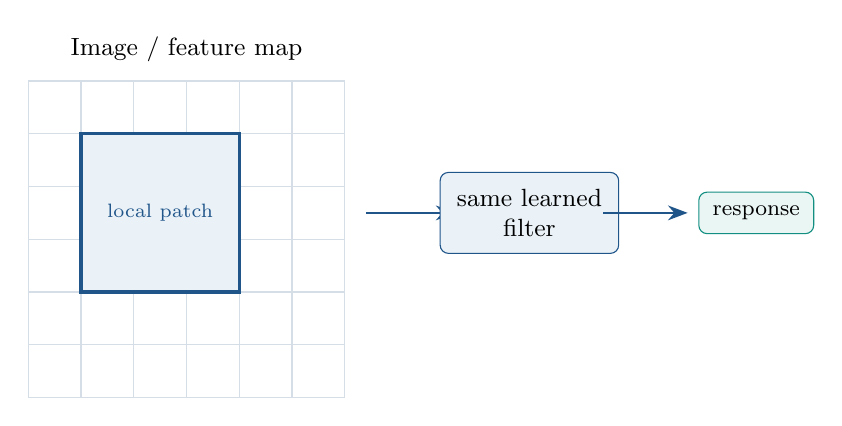
\begin{tikzpicture}[x=.67cm,y=.67cm]
    \foreach \x in {0,...,5}{\foreach \y in {0,...,5}{\draw[rulegray] (\x,\y) rectangle ++(1,1);}}
    \fill[palerblue] (1,2) rectangle (4,5);
    \draw[deepblue,very thick] (1,2) rectangle (4,5);
    \node[font=\small,align=center] at (3,6.6) {Image / feature map};
    \node[font=\scriptsize,deepblue] at (2.5,3.5) {local patch};
    \draw[arrblue] (6.4,3.5)--(8.1,3.5);
    \node[flow,minimum width=2.2cm] at (9.5,3.5) {same learned\\filter};
    \draw[arrblue] (10.9,3.5)--(12.5,3.5);
    \node[yesbox] at (13.8,3.5) {response};
    \end{tikzpicture}
    \caption{Convolution is easiest to read as one reusable local detector evaluated at many positions.}
\end{figure}

\paragraph{Channels are Functions}
RGB begins with three maps.
After a learned layer, the channels are better viewed as different feature maps: edge evidence, texture evidence, colour transitions, or more abstract learned patterns.
Later layers mix these channels into progressively richer evidence.


\begin{calloutmemoryhook}
A CNN reuses local pattern detectors across space.
\end{calloutmemoryhook}

\section{Receptive field, resolution and depth}
\label{sec:cnn-receptive-field}
A shallow unit sees a small patch; deeper units combine evidence from many earlier patches and therefore depend on a larger part of the input.
Depth builds a hierarchy from local evidence toward larger-context evidence.

\begin{figure}[htbp]
\centering
\begin{tikzpicture}[node distance=7mm and 9mm]
\node[flow] (p) {Pixels\\small patch};
\node[flow,right=of p] (e) {Edges /\\textures};
\node[flow,right=of e] (s) {Shapes /\\parts};
\node[yesbox,right=of s] (o) {Object-level\\evidence};
\draw[arr] (p)--(e);
\draw[arr] (e)--(s);
\draw[arr] (s)--(o);
\end{tikzpicture}
\caption{Stacking local operations increases effective context; the labels are a useful hierarchy intuition rather than fixed neuron semantics.}
\end{figure}

Stride and pooling reduce spatial resolution.
The practical trade-off is
\[
\underbrace{\text{high resolution}}_{\text{fine localisation, more memory/compute}}
\quad\longleftrightarrow\quad
\underbrace{\text{low resolution}}_{\text{cheaper, coarser spatial detail}}.
\]
Detection and segmentation usually care more about preserving location than image-level classification.

\section{Efficient convolution: separate spatial filtering from channel mixing}
\label{sec:cnn-depthwise-separable}
A standard convolution performs two jobs together: inspect local spatial structure and mix information across channels.
A \textbf{depthwise-separable convolution} factorises them:
\[
\boxed{
\text{spatial filtering per channel}
\ \longrightarrow\
\text{$1\times1$ channel mixing}
}.
\]
For a $3\times3$ layer with $64$ input and $128$ output channels, the rough per-position weight interaction count changes from
\[
\underbrace{3\times3\times64\times128}_{73{,}728\ \text{standard}}
\quad\longrightarrow\quad
\underbrace{3\times3\times64+64\times128}_{8{,}768\ \text{factorised}}.
\]
The reduction comes from a restriction: spatial and cross-channel reasoning are no longer represented by one unrestricted operation.
MobileNet-style architectures exploit this trade-off for resource-constrained inference.

\begin{calloutbias}
If spatial filtering and channel mixing can be approximately factorised, depthwise-separable convolution saves substantial compute; if their interaction must be richly coupled, the restriction can cost accuracy.
\end{calloutbias}

\section{Classification, detection and cheap classical stages}
\label{sec:cnn-classification-detection}
Classification maps an image to an image-level label.
Detection must additionally return locations, so its output is a set of boxes/classes/confidences rather than one class.

\begin{figure}[htbp]
\centering
\begin{tikzpicture}[node distance=8mm and 14mm]
\node[flow] (im1) {Image};
\node[flow,right=of im1] (cls) {Classifier};
\node[yesbox,right=of cls] (lab) {``dog''};
\node[flow,below=14mm of im1] (im2) {Image};
\node[flow,right=of im2] (det) {Detector};
\node[yesbox,right=of det] (boxes) {dog box\\ball box};
\draw[arr] (im1)--(cls);\draw[arr] (cls)--(lab);
\draw[arr] (im2)--(det);\draw[arr] (det)--(boxes);
\end{tikzpicture}
\caption{Classification asks what is present; detection asks what is present and where.}
\end{figure}

A learned model is not automatically the cheapest valid solution.
For a strongly coloured marker, HSV thresholding plus contour geometry can provide a fast first-stage detector:
\[
\text{RGB frame}
\rightarrow
\text{HSV}
\rightarrow
\text{colour threshold}
\rightarrow
\text{contours}
\rightarrow
\text{candidate location}.
\]
A production cascade can therefore begin with deterministic image structure and use a neural detector only for harder appearance variation.

\begin{calloutpractical}
Use the cheapest hypothesis class that captures the structure you actually need; a learned model should earn its extra flexibility.
\end{calloutpractical}

\section{Video: use time when single frames are ambiguous}
\label{sec:cnn-temporal}
Motion blur, occlusion or lighting can make one frame unreliable even when neighbouring frames are clear.
A temporal stage uses nearby observations to stabilise the decision:
\[
\underbrace{\hat y_t}_{\text{current decision}}
=
f(
\underbrace{x_{t-k:t}}_{\text{recent frames}}
).
\]
The useful assumption is that the physical scene evolves continuously enough for neighbouring frames to provide evidence about the present.

\begin{calloutbias}
If nearby frames describe one continuously evolving scene, temporal consistency can suppress transient visual noise; abrupt scene cuts or genuinely fast changes weaken that assumption.
\end{calloutbias}

\section{Pretrained visual representations: CLIP-like versus DINO-like}
\label{sec:cnn-pretrained-visual-representations}
The most important difference is the pretraining signal rather than the brand name.
A CLIP-like system aligns an image encoder with a text encoder:
\[
\text{image}
\rightarrow
z_{\text{image}}
\quad\text{close to}\quad
z_{\text{text}}
\leftarrow
\text{matching caption}.
\]
Its representation is therefore pressured toward linguistically describable semantics.
A DINO-like self-supervised visual encoder learns reusable image structure from transformed views without requiring paired captions.
Both can become backbones for a small downstream classifier; \cref{sec:adaptation-zero-shot-learning-no-task-specific-labelled-examples} gives the zero-shot image--text connection.

\begin{center}
\small
\begin{tabularx}{.94\linewidth}{@{}L{.23\linewidth}YY@{}}
\toprule
\textbf{Representation} & \textbf{Training pressure} & \textbf{Useful consequence} \\
\midrule
CLIP-like & Match paired image/text semantics & Language-aligned similarity and zero-shot prompts \\
DINO-like & Self-supervised consistency across image views & General visual features without captions \\
\bottomrule
\end{tabularx}
\end{center}

\section{How vision systems evolved}
\label{sec:cnn-evolution}
The useful evolution is an accumulation of constraints and reusable representation learning rather than a replacement ladder.

\begin{center}
\small
\begin{tabularx}{.97\linewidth}{@{}L{.18\linewidth}L{.22\linewidth}YY@{}}
\toprule
\textbf{Step} & \textbf{What changed} & \textbf{Problem targeted} & \textbf{New trade-off} \\
\midrule
Classical CV & Hand-written colour/geometry rules & Extremely cheap structured tasks & Brittle to appearance variation \\
CNN & Learn local shared filters & Hand-written feature limits & Training/data/compute cost \\
Residual/deeper CNN & Easier optimisation of depth & Need larger effective hierarchy & More compute \\
Depthwise conv. & Factorise spatial/channel work & Edge/mobile serving cost & More constrained layer \\
Pretrained encoder & Reuse broad learned representation & Limited labelled target data & Inherit pretraining bias \\
Multimodal/self-supervised & Broaden training signal & Reusable semantics without task labels & Larger pretraining systems \\
\bottomrule
\end{tabularx}
\end{center}

\begin{calloutdegreeofexperiment}
Vary input resolution, kernel/receptive-field design, depth, width, standard versus factorised convolution, downsampling schedule, pretrained backbone, temporal context and deployment precision.
\end{calloutdegreeofexperiment}

\chapter{Architecture: Transformers}
\label{chap:transformers}
\subsection{History}
At 2015, the world had:
\begin{itemize}
    \item How to represent workds? \textbf{Embeddings:} ELMo
    \item How to Process a sequence of data? \textbf{Reccurance:} RNNs
    \item How should our language modelling philosophy work? \textbf{General NN Modelling Approach:} ULM-FiT
\end{itemize}
But it was missing the answer to \textit{How do we relate points of the sequence to each other?} 
In CNNs the revolution happened already with AlexNet, and the answer to this question was the convolutional patterns.
Relationships between points in the image were encoded. 
However this does not map naturally to sequences, variable distances between points do not cause variable relationships between those points.
That is where attention was vital.


\section{Attention}
\label{sec:attention}
The layer receives a matrix of token representations:
\[
X\in\mathbb{R}^{N_{\text{tokens}}\times N_{\text{representation dims}}}.
\]
Project each token into three representations:
\[
Q=X\theta_{\text{query}},\qquad
K=X\theta_{\text{key}},\qquad
V=X\theta_{\text{value}}.
\]
The query from the target token is compared to every other token's key through the dot product.
The most basic version of the equation looks like
\[
\underbrace{\operatorname{Attention}(Q,K,V)}_{\text{context gathered for each token}}
=
\underbrace{
\softmax\!\left(
\frac{\overbrace{QK^\top}^{\text{query--key compatibility}}}
{\sqrt{N_{\text{key dims}}}} + M_{\text{allowed routes}}
\right)
}_{\text{who should I listen to?}}
\underbrace{V}_{\text{what do they say?}}
.
\]

\begin{center}
\small
\begin{tabularx}{.92\linewidth}{@{}L{.18\linewidth}Y@{}}
\toprule
\textbf{Term} & \textbf{Intuition} \\
\midrule
$Q$ & ``What am I looking for?'' \\
$K$ & ``What information do I contain?'' \\
$QK^\top$ & compatibility between every query and key \\
$V$ & information actually retrieved \\
$M_{\text{allowed routes}}$ & optional mask saying which interactions are allowed \\
$N_{\text{key dims}}$ & width of each key/query vector \\
\bottomrule
\end{tabularx}
\end{center}
A token can now ask \textit{Which other tokens contain information relevant to what I currently need?}
The matching representation and the retrieved representation are deliberately separate: $K$ decides whether a token is relevant, while $V$ decides what information it sends.
The division by $\sqrt{N_{\text{key dims}}}$ keeps dot-product magnitudes from growing with representation width and pushing softmax too quickly toward a near winner-take-all distribution.

\begin{calloutbias}
If useful interactions depend on token content, attention can learn the routes dynamically.
If most useful interaction is local or compressible, unrestricted all-pairs attention may spend unnecessary compute.
\end{calloutbias}

\subsection{Problem Definition}
Before attention, neural sequence-to-sequence models commonly compressed an input sequence through recurrent state before decoding an output sequence.
Conceptually,
\[
\underbrace{x_1,x_2,\ldots,x_{N_{\text{input}}}}_{\text{source sequence}}
\longrightarrow
\underbrace{h_{\text{final}}}_{\text{one compressed source representation}}
\longrightarrow
\underbrace{y_1,y_2,\ldots}_{\text{generated sequence}}.
\]
The failure mode is obvious for long inputs: one state must preserve every detail that any later decoder step might need.

Early \textbf{encoder--decoder attention} kept the encoder states available and let each decoder step retrieve a different weighted combination:
\[
\underbrace{c_t}_{\text{information retrieved at decoder step }t}
=
\sum_i
\underbrace{
\softmax\!\left(
\operatorname{compatibility}(s_{t-1},h_i)
\right)
}_{\text{how useful is source state }i\text{ now?}}
\underbrace{h_i}_{\text{stored source information}}.
\]
Bahdanau-style \textbf{additive attention} learned the compatibility function with a small neural network.
Luong-style \textbf{multiplicative attention} showed that compatibility could instead be built around a dot product, moving the mechanism toward the matrix-multiplication-friendly $QK^\top$ form used by Transformers.

\begin{calloutmemoryhook}
Attention began as a way for a decoder to retrieve different encoder states instead of trusting one fixed summary of the whole source.
\end{calloutmemoryhook}

\subsubsection{Attention Hardness}
\textbf{Soft attention} forms a differentiable weighted mixture of candidates:
\[
\text{retrieved information}
=
\sum_i
\underbrace{\alpha_i}_{\text{continuous weight}}
\underbrace{v_i}_{\text{candidate information}}.
\]
This is the default meaning of attention in modern Transformers.

\textbf{Hard attention} instead selects one or a small number of locations.
That can avoid processing every candidate at high resolution, but discrete selection is harder to optimise with ordinary backpropagation.
Modern learned sparse attention revisits the same broad systems question---\textit{which memories are worth paying expensive retrieval compute for?}---without being identical to early hard attention.

\subsection{Experiment Dimensions}
\label{sec:modern-attention-variants}
Attention terminology becomes confusing because several ideas called ``attention variants'' actually change completely different parts of the system.

\begin{center}
\small
\begin{tabularx}{.96\linewidth}{@{}L{.24\linewidth}L{.28\linewidth}Y@{}}
\toprule
\textbf{Design question} & \textbf{Examples} & \textbf{What changes} \\
\midrule
Where do $K,V$ come from? & self / cross & information source / architecture \\
Which positions may interact? & causal / bidirectional & information-flow constraint \\
Which pairs are considered? & full / local / sparse & connectivity and compute \\
How is compatibility computed? & additive / dot-product / kernelised & matching function \\
How many $K,V$ heads exist? & MHA / GQA / MQA & KV-cache size and head sharing \\
How is KV memory stored? & explicit KV / MLA latent & representation stored during decoding \\
How is history represented? & explicit tokens / recurrent state / hybrid & exact retrieval versus compression \\
How is attention executed? & naive / FlashAttention & hardware algorithm, not model semantics \\
\bottomrule
\end{tabularx}
\end{center}

\subsubsection{Self-attention and cross-attention}
\label{subsec:modern-cross-attention}
Self-attention means
\[
Q\leftarrow\text{sequence A},
\qquad
K,V\leftarrow\text{sequence A}.
\]
The sequence uses content-dependent retrieval to communicate with itself.

Cross-attention instead means
\[
Q\leftarrow\text{sequence A},
\qquad
K,V\leftarrow\text{sequence B}.
\]

\begin{figure}[htbp]
\centering
\begin{tikzpicture}[node distance=8mm and 14mm]
\node[flow] (enc) {English encoder\\``The dog runs''};
\node[yesbox,right=of enc] (kv) {$K,V$};
\node[flow,right=of kv] (att) {Cross-attention};
\node[yesbox,below=8mm of att] (q) {$Q$};
\node[flow,left=of q] (dec) {French decoder\\``Le chien ...''};
\draw[arr] (enc)--(kv);
\draw[arr] (kv)--(att);
\draw[arr] (dec)--(q);
\draw[arr] (q)--(att);
\end{tikzpicture}
\caption{Cross-attention lets one representation query information stored in another representation.}
\label{fig:modern-cross-attention}
\end{figure}

The decoder asks \textit{Given what I am currently generating, which information in the encoded source do I need?}
That is \textbf{cross-attention}.
It becomes especially important when we reach Perceiver in \cref{subsec:modern-perceiver}, because Perceiver uses cross-attention to map a huge input into a small latent representation.
The same pattern is also useful for multimodal systems, where text representations may query image/audio representations or vice versa.

\subsubsection{Causal Masking}
\label{sec:transformers-causal-mask}
A global attention mechanism would see all tokens, and not just historical ones, causing lookahead bias.
Causal masks permit only earlier/current positions.

\begin{center}
\small
\begin{tabular}{c|ccccc}
 & key 1 & key 2 & key 3 & key 4 & key 5\\
\hline
query 1 & $\checkmark$ & $\times$ & $\times$ & $\times$ & $\times$\\
query 2 & $\checkmark$ & $\checkmark$ & $\times$ & $\times$ & $\times$\\
query 3 & $\checkmark$ & $\checkmark$ & $\checkmark$ & $\times$ & $\times$\\
query 4 & $\checkmark$ & $\checkmark$ & $\checkmark$ & $\checkmark$ & $\times$\\
query 5 & $\checkmark$ & $\checkmark$ & $\checkmark$ & $\checkmark$ & $\checkmark$\\
\end{tabular}
\end{center}

\begin{calloutmemoryhook}
The causal mask assigns attention scores of future keys to $-\infty$, so the softmax pushes them to 0.
\end{calloutmemoryhook}

\subsection{Multi-Head Attention}
Most applications learn multiple versions of the attention mechanism and combine them.
\[
\underbrace{\operatorname{MultiHeadAttention}(Q,K,V,H)}_{\text{context gathered for each token}}
=
\operatorname{Agg}\!\left[
\operatorname{Attention}(Q,K,V)_{\text{Head 1}},\ldots,
\operatorname{Attention}(Q,K,V)_{\text{Head }H}
\right].
\]
Each head has its own learned query/key/value projections, so each can implement a different retrieval geometry.
Do not interpret that too literally as ``one head learns syntax, one head learns names'': useful computation can be redundant or distributed across heads.

\begin{figure}[htbp]
\centering
\begin{tikzpicture}[node distance=7mm and 11mm]
\node[flow] (x) {Token representations};
\node[yesbox,below left=9mm and 20mm of x] (h1) {Head 1};
\node[yesbox,below=9mm of x] (h2) {Head 2};
\node[yesbox,below right=9mm and 20mm of x] (h3) {Head $H$};
\node[flow,below=17mm of h2] (agg) {Concatenate / aggregate};
\node[flow,below=8mm of agg] (out) {Output projection};
\draw[arr] (x)--(h1);
\draw[arr] (x)--(h2);
\draw[arr] (x)--(h3);
\draw[arr] (h1)--(agg);
\draw[arr] (h2)--(agg);
\draw[arr] (h3)--(agg);
\draw[arr] (agg)--(out);
\end{tikzpicture}
\caption{Multi-head attention learns several retrieval geometries in parallel before recombining them.}
\label{fig:modern-multihead-attention}
\end{figure}

\subsection{Problems with Attention}
The Transformer removes the recurrent bottleneck by keeping token representations explicitly addressable.
Token 1000 can retrieve token 1 through one attention operation rather than forcing information through 999 recurrent state updates.
The price is that explicit memory creates two separate scaling problems.

\paragraph{Problem 1: dense pairwise interaction.}
For sequence length $N_{\text{tokens}}$,
\[
\underbrace{QK^\top}_{\text{pairwise compatibility}}
\in
\mathbb{R}^{N_{\text{tokens}}\times N_{\text{tokens}}},
\qquad
\text{attention arithmetic}
\sim
O\!\left(N_{\text{tokens}}^2N_{\text{head dims}}\right).
\]
This motivates local attention, sparse attention and linear/stateful alternatives.

\paragraph{Problem 2: autoregressive KV cache.}
During generation, keys and values from previous tokens are cached so they do not need to be recomputed for every new token.
Very roughly,
\[
\underbrace{\text{KV cache size}}_{\text{stored decoding memory}}
\propto
N_{\text{tokens}}
\times
N_{\text{KV heads}}
\times
N_{\text{head dims}}.
\]
This motivates MQA, GQA and MLA.

\begin{calloutmemoryhook}
Sparse/linear attention mainly attacks how many sequence interactions are computed; MQA/GQA/MLA mainly attack how much key/value memory must be stored or moved.
\end{calloutmemoryhook}

\subsection{KV Optimisation Developments}
\label{subsec:modern-kv-attention-evolution}
These methods (MHA $\rightarrow$ MQA $\rightarrow$ GQA $\rightarrow$ MLA) are easiest to understand as an evolution of the KV-cache problem.

\subsubsection{Multi-Query Attention}
Standard multi-head attention shares all keys and values, giving every query head its own key/value head:
\[
(Q_1,K_1,V_1),\ (Q_2,K_2,V_2),\ldots,(Q_H,K_H,V_H).
\]
\textbf{Multi-Query Attention (MQA)} keeps multiple query heads but shares one $K,V$ representation:
\[
Q_1,Q_2,\ldots,Q_H
\quad\longrightarrow\quad
K_{\text{shared}},V_{\text{shared}}.
\]
This can radically reduce KV-cache memory traffic during autoregressive decoding.
The trade-off is less head-specific key/value representation capacity.

\begin{calloutbias}
If several query heads can retrieve successfully from a common key/value representation, separate $K,V$ heads are redundant; if heads need genuinely different retrieval memories, full sharing can be restrictive.
\end{calloutbias}

\subsubsection{Grouped Query Attention}
\textbf{Grouped Query Attention (GQA)} makes sharing a continuum, stopping treating KV sharing as all-or-nothing.
Several query heads share each key/value head:
\[
1
<
N_{\text{KV heads}}
<
N_{\text{query heads}}.
\]
The endpoints recover familiar cases:
\[
N_{\text{KV heads}}=N_{\text{query heads}}
\Rightarrow
\text{MHA},
\qquad
N_{\text{KV heads}}=1
\Rightarrow
\text{MQA}.
\]
So $N_{\text{KV heads}}$ is a direct efficiency--capacity design knob rather than three unrelated algorithms.
Later Llama, Mistral and Qwen-family models provide prominent examples of GQA-style decoder designs, although exact choices vary by model version.

\subsubsection{Multi-Head Latent Attention}
\textbf{Multi-Head Latent Attention (MLA)} attacks the same decoding-memory problem differently; by compressing what is cached.
Instead of merely sharing full $K,V$ heads, compress the token's KV information into a smaller latent representation:
\[
\underbrace{x_t}_{\text{token representation}}
\longrightarrow
\underbrace{c_t^{KV}}_{\text{small cached latent}}
\longrightarrow
\underbrace{K_t,V_t}_{\text{information needed by attention}}.
\]
MLA is therefore better remembered as \textit{compress the KV memory} rather than \textit{share more heads}.
DeepSeek-V2 introduced MLA, and later DeepSeek models build on the same broad memory-efficiency lineage.

\begin{calloutmemoryhook}
MQA/GQA share KV representations; MLA compresses the representation that must be cached.
\end{calloutmemoryhook}

\subsection{Attention Sparsity}
Dense attention assumes any pair of sequence elements might require a direct interaction.
That flexibility is useful, but a long sequence spends compute on $N_{\text{tokens}}^2$ candidate pairs even if most are unimportant.

\subsubsection{Local / sliding-window attention}
The simplest stronger bias is locality: each query attends only to a nearby window of $N_{\text{window}}$ keys.
The interaction cost becomes roughly
\[
O\!\left(N_{\text{tokens}}N_{\text{window}}N_{\text{head dims}}\right)
\qquad
\text{instead of}
\qquad
O\!\left(N_{\text{tokens}}^2N_{\text{head dims}}\right).
\]
This is attractive when useful dependencies are predominantly local, as in many image, audio and time-series settings.
The failure mode is direct: an important distant token may be outside the allowed window.

\begin{calloutbias}
If useful interactions are mostly local, windowed attention spends explicit retrieval compute where it is most valuable; if arbitrary distant details matter, the window becomes an information-routing bottleneck.
\end{calloutbias}

\subsubsection{Structured sparse attention}
Methods such as Sparse Transformer, Longformer and BigBird keep explicit token memory but allow only a designed subset of interactions.
Typical patterns combine local windows with occasional global, strided or random long-range routes.
The useful abstraction is
\[
\underbrace{\text{keep explicit history}}_{\text{token-level memory}}
+
\underbrace{\text{search only part of it}}_{\text{sparse connectivity}}.
\]
Reformer explores a related content-based route: hash similar representations into buckets and concentrate attention within likely-relevant buckets.
Linformer instead assumes the interaction structure is sufficiently low-rank to compress the sequence dimension before expensive attention.

\subsection{Linear Attention and Recurrent Memory}
Sparse attention keeps explicit token memories but searches fewer of them.
\textbf{Linear attention} goes further by replacing/rearranging the interaction so that history can be accumulated into a compact state rather than materialising an $N_{\text{tokens}}\times N_{\text{tokens}}$ matrix.
Schematically, with a feature map $\phi(\cdot)$ and normalisation omitted,
\[
\underbrace{\phi(Q)\phi(K)^\top V}_{\text{pairwise form}}
=
\underbrace{\phi(Q)\left(\phi(K)^\top V\right)}_{\text{summarise keys/values first}}.
\]
The parenthesisation changes the computation dramatically.
Instead of building all query--key pairs, first build a compact key/value summary and let queries read that summary.

For causal processing this can become a recurrent update:
\[
\underbrace{S_t}_{\text{memory after token }t}
=
\underbrace{S_{t-1}}_{\text{previous memory}}
+
\underbrace{\phi(k_t)v_t^\top}_{\text{new association}},
\qquad
\underbrace{y_t}_{\text{retrieved output}}
\propto
\phi(q_t)^\top S_t.
\]
This exposes the important connection:
\[
\boxed{\text{some linear-attention formulations are recurrent matrix memories}.}
\]
Performer is one route that approximates softmax attention with feature maps while avoiding an explicit quadratic attention matrix.

\subsubsection{Why linear/stateful memory does not simply dominate full attention}
Dense attention keeps previous token representations individually addressable.
A recurrent state instead continually compresses the past.
So the fundamental trade-off is
\[
\underbrace{\text{explicit token memory}}_{\text{precise content-addressed retrieval}}
\quad\longleftrightarrow\quad
\underbrace{\text{compressed state}}_{\text{bounded efficient memory}}.
\]
Exact retrieval of an old detail is natural on the left and must have survived compression on the right.
This is why efficient recurrent/linear architectures can be excellent long-sequence processors without making dense attention obsolete.

\subsubsection{Mamba is not attention}
Mamba belongs to the state-space/recurrent branch rather than ordinary softmax attention.
The basic data flow is
\[
\text{new token}
+
\text{previous state}
\longrightarrow
\text{updated state},
\]
so past information is carried through an evolving finite state rather than an ever-growing list of cached token keys/values.
Mamba's important addition over earlier structured state-space models is \textbf{selectivity}: the current input can influence what is written, retained or forgotten.
The S4/Mamba mechanism is developed in the sequence-model evolution section below; the point here is where it sits in the attention design space.

\begin{calloutmemoryhook}
Transformer attention stores history for later search; Mamba-style recurrence continually updates a compressed memory of history.
\end{calloutmemoryhook}

Mamba-2 / Structured State Space Duality makes the boundary less clean by showing close mathematical links between structured state-space transformations and attention-like sequence operations.
DeltaNet-style linear attention explores the same middle ground through a recurrent matrix memory with targeted \textbf{delta updates} rather than only accumulating new associations.
Gated DeltaNet adds adaptive forgetting, giving the state both \textit{what should be overwritten?} and \textit{how quickly should old memory decay?} controls.

\subsection{FlashAttention}
\label{subsec:modern-flashattention}
FlashAttention is really just a wacky implementation of ordinary dense self-attention, but it deserves its own section because it attacks a completely different bottleneck.

\paragraph{Dense Matrix Materialisation Bottleneck.}
Vanilla attention generates lots of large $N_{\text{tokens}}\times N_{\text{tokens}}$ matrices.
\begin{figure}[htbp]
\centering
\begin{tikzpicture}[node distance=8mm]
\node[flow] (qk) {$Q,K$};
\node[flow,right=of qk] (scores) {Compute enormous\\$QK^\top$ matrix};
\node[yesbox,right=of scores] (write1) {Write scores to\\GPU HBM};
\node[flow,right=of write1] (soft) {Read scores\\+ softmax};
\node[yesbox,right=of soft] (write2) {Write probabilities\\to HBM};
\node[flow,right=of write2] (v) {Read probabilities\\+ multiply by $V$};

\draw[arr] (qk) -- (scores);
\draw[arr] (scores) -- (write1);
\draw[arr] (write1) -- (soft);
\draw[arr] (soft) -- (write2);
\draw[arr] (write2) -- (v);
\end{tikzpicture}
\caption{Naive attention repeatedly materialises large intermediate matrices in relatively slow high-bandwidth memory.}
\label{fig:modern-naive-attention-io}
\end{figure}

For sequence length $N_{\text{tokens}}$, the attention matrix is
\[
N_{\text{tokens}}\times N_{\text{tokens}}.
\]
At $N_{\text{tokens}}=16{,}384$:
\[
N_{\text{tokens}}^2
\approx
268\text{ million entries}
\]
per head/batch combination.
Moving those matrices backwards and forwards through GPU memory is expensive.
Modern accelerators can perform arithmetic extraordinarily quickly.
Often the bottleneck is \textbf{moving data rather than doing arithmetic}.

The important distinction is
\[
\underbrace{\text{dense attention arithmetic}}_{\text{still roughly }O(N_{\text{tokens}}^2N_{\text{head dims}})}
\qquad\text{but}\qquad
\underbrace{\text{HBM traffic / intermediate materialisation}}_{\text{can be reduced dramatically}}.
\]

\paragraph{Solution: FlashAttention.}
Break $Q$, $K$ and $V$ into tiles small enough to fit in fast on-chip memory.

\begin{figure}[htbp]
\centering
\begin{tikzpicture}[node distance=8mm and 18mm]
\node[yesbox] (hbm) {Large / slower\\HBM};
\node[flow,right=of hbm] (tile) {Load small\\$Q,K,V$ tiles};
\node[yesbox,right=of tile] (sram) {Fast on-chip\\SRAM};
\node[flow,below=10mm of sram] (calc) {Compute score tile\\update online softmax\\accumulate output};
\node[yesbox,left=of calc] (out) {Small accumulated\\state / output};
\draw[arr] (hbm)--(tile);
\draw[arr] (tile)--(sram);
\draw[arr] (sram)--(calc);
\draw[arr] (calc)--(out);
\draw[arr,rounded corners] (calc.east)--++(.7,0)--++(0,1.0)--(sram.east);
\end{tikzpicture}
\caption{FlashAttention tiles the exact attention computation so large score/probability matrices do not need to be repeatedly materialised in HBM.}
\label{fig:modern-flashattention-tiling}
\end{figure}

Softmax can be maintained incrementally, so the $N_{\text{tokens}}\times N_{\text{tokens}}$ attention matrix never needs to be materialised in HBM.
Roughly,
\[
\text{FLOPs}
\sim
O(N_{\text{tokens}}^2N_{\text{head dims}}),
\]
just like ordinary dense attention at the algorithmic level.
The speedup comes from IO-aware scheduling, tiling and avoiding wasteful reads/writes of enormous intermediates.

\begin{calloutmemoryhook}
Sparse or linear attention changes the mathematical interaction structure; FlashAttention computes ordinary attention more efficiently.
\end{calloutmemoryhook}

\subsection{Learned Sparse Attention}
Here we let the Model Decide What Is Worth Reading.
Hand-designed sparse attention says in advance which routes are cheap enough to keep.
A more modern question is: \textit{can the model learn which old memories deserve expensive high-resolution attention?}

\textbf{Native Sparse Attention (NSA)} combines several resolutions of memory: a compressed global view, selected important tokens/blocks and a local window.
The broad design is
\[
\underbrace{\text{compressed global context}}_{\text{cheap broad awareness}}
+
\underbrace{\text{selected fine detail}}_{\text{content-dependent retrieval}}
+
\underbrace{\text{local window}}_{\text{precise recent context}}.
\]

\textbf{DeepSeek Sparse Attention (DSA)} similarly introduces a lightweight selection/indexing stage so expensive attention is concentrated on a smaller relevant subset of historical tokens.
The important evolution is
\[
\text{full attention}
\rightarrow
\text{fixed sparse pattern}
\rightarrow
\text{learn which memories are worth reading}.
\]

\begin{calloutbias}
If only a small fraction of distant history is useful for each query, learned sparse routing can preserve explicit retrieval while avoiding most pairwise work; if the selector misses an important memory, sparsity itself becomes the failure mode.
\end{calloutbias}

\subsection{Modern Hybrids}
This allows for Compressed Memory Most of the Time, Explicit Retrieval Sometimes.
Full attention is good at precise content-addressed retrieval but expensive.
Linear/recurrent memory is efficient but compresses history.
A natural compromise is therefore to use cheap recurrent/linear sequence mixing in most layers and retain occasional full-attention layers for exact retrieval.

\begin{figure}[htbp]
\centering
\begin{tikzpicture}[node distance=6mm]
\node[flow] (l1) {Linear / recurrent memory};
\node[flow,below=of l1] (l2) {Linear / recurrent memory};
\node[flow,below=of l2] (l3) {Linear / recurrent memory};
\node[yesbox,below=of l3] (att) {Full attention};
\node[flow,below=of att] (rep) {Repeat};
\draw[arr] (l1)--(l2);
\draw[arr] (l2)--(l3);
\draw[arr] (l3)--(att);
\draw[arr] (att)--(rep);
\end{tikzpicture}
\caption{A common modern compromise: compressed/stateful processing handles most layers, while occasional attention restores high-resolution token retrieval.}
\label{fig:modern-hybrid-attention}
\end{figure}

Jamba is an early large-scale example of mixing Mamba-style blocks with Transformer attention.
Qwen3-Next uses a $3{:}1$ mixture of Gated DeltaNet layers to gated full-attention layers, explicitly targeting the efficiency--recall trade-off.
Qwen3.5 carries that broad Qwen3-Next hybrid architecture into a 2026 natively multimodal model family.
Kimi Linear similarly combines \textbf{Kimi Delta Attention (KDA)}---a Gated DeltaNet-like linear attention mechanism---with occasional MLA layers.
DeepSeek-V4 represents a different long-context route: token-wise compression combined with DSA rather than primarily replacing attention with recurrent state.

\begin{calloutmemoryhook}
Modern hybrids assume most history can be compressed cheaply, but some layers still benefit from direct high-resolution retrieval over explicit tokens.
\end{calloutmemoryhook}

\subsection{Applications}
The attention equation is modality-agnostic.
The main application question is not ``is this language or medicine?'' but \textit{what counts as a token, what relationships matter, and how much history must remain explicitly addressable?}

\begin{center}
\small
\begin{tabularx}{.96\linewidth}{@{}L{.18\linewidth}L{.32\linewidth}Y@{}}
\toprule
\textbf{Domain} & \textbf{Typical token / memory unit} & \textbf{Useful attention choices} \\
\midrule
LLMs & subword/token representations & causal self-attention; GQA/MQA/MLA for KV efficiency; sparse or hybrid mechanisms for long context \\
Encoder NLP & words/subwords / document chunks & bidirectional self-attention; local/global sparse attention for long documents \\
Vision & image patches / regions & global ViT attention when long-range interaction matters; windowed/local attention when spatial locality is strong \\
Multimodal & text tokens + image/audio/video tokens & cross-attention or early-fused self-attention across modalities \\
Time series & timesteps, temporal patches or variables & temporal attention, sparse attention, patch tokenisation, or SSM/Mamba-like state for very long streams \\
Medical EHR & visits, diagnoses, medications, labs, note tokens & long-range self-attention when distant events may matter; sparse/long-context variants for large patient histories \\
Medical imaging & 2-D/3-D patches & ViT/Swin/UNETR-style attention for global context; windowed attention or Mamba-like state-space blocks when full spatial attention is too expensive \\
\bottomrule
\end{tabularx}
\end{center}

\paragraph{Time-series optionality.}
Informer-style methods make attention sparse because only a subset of temporal interactions is expected to dominate.
PatchTST instead reduces $N_{\text{tokens}}$ by grouping neighbouring timesteps into temporal patches before applying attention.
iTransformer changes a different axis again: variables/channels become the attended tokens, so attention learns relationships between variables rather than treating every timestamp as the primary token unit.
The lesson is that changing \textbf{what becomes a token} can be as important as changing the attention equation.

\paragraph{Medical examples.}
Transformer-style models such as BEHRT/Med-BERT treat longitudinal health-record events as a sequence where a later prediction can retrieve relevant earlier diagnoses, medications or visits.
Clinical long-document models reuse sparse long-context attention ideas for notes.
UNETR/Swin-like models use attention over image/volume patches, while VM-UNet/Mamba-UNet-style work explores state-space alternatives when dense spatial attention is too expensive.
These are applications of the same sequence-memory choices rather than a separate ``medical attention'' mechanism.

\subsection{Research Evolution: How Much of the Past Stays Explicitly Addressable?}
The useful history is not a straight line where one mechanism replaces the previous one.
It is a branching accumulation of fixes around retrieval, memory and hardware cost.

\begin{center}
\scriptsize
\begin{tabularx}{.98\linewidth}{@{}L{.18\linewidth}L{.24\linewidth}L{.27\linewidth}Y@{}}
\toprule
\textbf{Step} & \textbf{What changed} & \textbf{Problem targeted} & \textbf{New trade-off} \\
\midrule
Fixed-state seq2seq & compress source into recurrent state & sequence-to-sequence modelling & one-state information bottleneck \\
Bahdanau attention & retrieve different encoder states per decoder step & fixed source bottleneck & explicit source memory + matching cost \\
Luong / dot-product attention & cheaper multiplicative compatibility & efficient matching & still attached to recurrent encoder/decoder \\
Transformer & self-attention becomes main sequence mixer & long recurrent paths / parallel training & dense $N_{\text{tokens}}^2$ interaction \\
Sparse/local attention & compute only structured subset of pairs & long-context cost & stronger connectivity assumptions \\
MQA & share one KV head across query heads & decode memory bandwidth & less head-specific KV capacity \\
GQA & use intermediate number of KV heads & MHA quality vs MQA efficiency & another capacity/efficiency knob \\
Linear / low-rank attention & summarise/compress interactions before retrieval & quadratic pairwise cost & less direct exact token access \\
FlashAttention & tile exact dense attention around memory hierarchy & HBM traffic / intermediates & arithmetic remains dense \\
Mamba / Mamba-2 & selective/structured recurrent state & long-sequence memory and streaming & history is compressed into finite state \\
MLA & compress KV into a latent before caching & KV-cache size & learned compression machinery \\
Gated DeltaNet / KDA & richer gated recurrent memory updates & linear-memory recall and overwriting & finite-state bottleneck remains \\
NSA / DSA & learn which old memories deserve expensive retrieval & long-context dense attention & selector/routing can miss information \\
Modern hybrids & mix recurrent/linear memory with occasional full attention & efficiency versus exact recall & more architectural/kernel complexity \\
\bottomrule
\end{tabularx}
\end{center}

A useful genealogy is therefore
\[
\begin{array}{c}
\text{RNN fixed state}
\rightarrow
\text{attention on RNNs}
\rightarrow
\text{Transformer}\\[1mm]
\quad\searrow\ \text{local / sparse / learned sparse}\\
\quad\searrow\ \text{MHA}\rightarrow\text{MQA/GQA}\rightarrow\text{MLA}\\
\quad\searrow\ \text{linear attention}\leftrightarrow\text{SSM/Mamba}\rightarrow\text{Gated DeltaNet/KDA}\\
\quad\searrow\ \text{hybrids: Jamba, Qwen3-Next/Qwen3.5, Kimi Linear}.
\end{array}
\]
FlashAttention sits across this map as an execution optimisation for attention computations rather than another memory semantics.

\subsection{Research Optionality: What Exactly Can Be Changed?}
For attention research, avoid asking only \textit{Which attention mechanism is best?}
Ask which layer of the design is being changed.

\begin{center}
\small
\begin{tabularx}{.96\linewidth}{@{}L{.28\linewidth}Y@{}}
\toprule
\textbf{Degree of experiment} & \textbf{Choices} \\
\midrule
Information source & self-attention, cross-attention, multimodal source \\
Information direction & causal, bidirectional, prefix/structured masks \\
Connectivity & global, windowed, block sparse, learned sparse \\
Compatibility & additive, dot-product, kernel/feature-map approximation \\
Query/KV head sharing & MHA, GQA, MQA; vary $N_{\text{KV heads}}$ \\
KV representation & explicit heads, shared heads, latent-compressed MLA-style memory \\
History representation & explicit token cache, latent bottleneck, recurrent/SSM state, hybrid \\
State update & additive, gated, delta-rule / overwrite-like update \\
Token granularity & subword, image patch, time patch, variable, event, latent \\
Layer mixture & all attention, all state-space/linear, alternating or $k{:}1$ hybrid \\
Execution & naive kernels, tiling/fusion, FlashAttention-like implementation, precision/cache layout \\
\bottomrule
\end{tabularx}
\end{center}

\begin{calloutmemoryhook}
Attention evolution is mostly the history of deciding how much of the past stays explicitly addressable: full attention keeps and searches it, sparse attention keeps but searches less, recurrent/linear methods compress it, and modern hybrids do both.
\end{calloutmemoryhook}






\section{Residual Networks}



\section{Transformer Block}
\label{sec:modern-transformer}
In practice, you'll find many variations of the transformer block. Design choices include the placement, type and number of normalization layers, the exact MLP structure (gated vs. non-gated, the choice of gating function, etc.), residual connections structure (identity, Attention Residuals [4], etc.), and especially the attention module.

Broadly, attention mechanisms are either quadratic (e.g. MLA [5], scaled dot-product attn, etc.) or linear (e.g. Kimi Linear [6]) in sequence length, each with trade-offs between modeling capacity (especially at long context) and efficiency.

MoE, Muon (the optimizer [12]), and several architectural innovations such as MLA (DeepSeek), MTP (multi-token prediction), and DSA (sparse attention [13]).

A Transformer instead gives tokens direct communication paths.
Token 1000 can retrieve information from token 1 in essentially one attention operation.

\begin{calloutbias}
If arbitrary pairwise interactions between sequence elements may be useful, direct content-addressed attention gives flexible short paths; the cost is explicit memory and dense pairwise interaction.
\end{calloutbias}

This is much weaker than recurrence's assumptions.
It makes Transformers highly flexible.
But there is a cost:
\[
N_{\text{tokens}}
\quad\Rightarrow\quad
N_{\text{tokens}}^2\text{ pair interactions}.
\]

During autoregressive generation, ordinary attention usually also needs a cache of previous keys/values whose size grows with context length; see \cref{sec:inference-kv-cache}.





\section{Evolution}




Once researchers merged Attention into Residual connections between transformer blocks, several developments furthered the field.
We can ask the more interesting architectural question, \textit{How should information propagate through a sequence?}
There are three major mental models relevant to these topics:
\[
    \boxed{
    \begin{array}{lll}
    \text{RNN} &:& \text{history}\rightarrow\text{fixed state}\rightarrow\text{next state}\\
    \text{Transformer} &:& \text{tokens}\leftrightarrow\text{direct content-based interactions}\\
    \text{S4 / state-space} &:& \text{input drives a learned dynamical system}
    \end{array}
    }
\]
The baseline RNN mechanism is also in \cref{sec:models-rnns-sequential-state}; the baseline Transformer bias is in \cref{sec:models-transformers-content-dependent-interaction}.




TransformersXL, XLNet, BERT, RoBERTa, ALBERT, T5, UniLM, SparseTransformer, Longformer, Reformer, Linformer, SNAIL.

\subsection{Direction of Attention}
The original BERT models used bi-directional attention.
In practice, model must only see the past, and so masking was introduced. 

\subsection{Data Scale}
\label{subsec:modern-kaplan-chinchilla}
This is a useful historical evolution.
Earlier scaling work encouraged the intuition that very large models could be compute-efficient even when trained for fewer tokens than later practice would favour.
Then compute-optimal scaling was revisited with broader experiments.
The Chinchilla result made the practical point that many contemporary large models were undertrained relative to their size and that model size and training-token count should be scaled together much more aggressively than earlier practice.

Its famous comparison was approximately:
\[
\underbrace{280\text{B parameters}}_{\text{Gopher: larger model, less data}}
\qquad\text{vs.}\qquad
\underbrace{70\text{B parameters}}_{\text{Chinchilla: smaller model, much more data}}
\]
with similar training compute, where the more data-rich allocation performed better across many evaluations.

The lesson is not ``70B is optimal''.
That would be memorising a historical result incorrectly.

\begin{calloutmemoryhook}
Model size without enough training data is wasted capacity; data without enough model capacity eventually hits a model bottleneck.
\end{calloutmemoryhook}

The researcher's problem is to balance the two under constraints.








A separate scaling/training branch is:
\[
\begin{aligned}
\text{dense Transformer}
&\rightarrow
\text{empirical scaling laws}
\rightarrow
\text{compute-optimal allocation}\\
&\rightarrow
\text{MoE / sparse conditional computation}
\end{aligned}
\]
and
\[
\text{pretraining}
\rightarrow
\text{SFT}
\rightarrow
\text{LoRA / efficient adaptation}
\rightarrow
\text{preference optimisation / RLHF}
\rightarrow
\text{decoding}.
\]






\subsection{Context Fragmentation}
\label{subsec:modern-transformer-xl}
Vanilla Transformer language modelling historically had a frustrating problem.
Suppose training uses blocks of 512 tokens:
\[
\underbrace{[1\ldots512]}_{\text{segment 1}}
\qquad
\underbrace{[513\ldots1024]}_{\text{segment 2}}.
\]

When processing segment 2, vanilla chunked training can treat segment 1 as gone.
That causes \textbf{}.

Transformer-XL's solution:

\begin{quote}
Reuse hidden states from the previous segment as memory.
\end{quote}

Conceptually:

\begin{figure}[htbp]
\centering
\begin{tikzpicture}[node distance=8mm and 14mm]
\node[yesbox] (prev) {Previous segment\\hidden states};
\node[flow,right=of prev] (cache) {Cache / stop-gradient\\memory};
\node[flow,right=of cache] (att) {Current segment\\attention};
\node[yesbox,below=8mm of att] (cur) {Current segment\\states};
\draw[arr] (prev)--(cache);
\draw[arr] (cache)--(att);
\draw[arr] (cur)--(att);
\end{tikzpicture}
\caption{Transformer-XL extends the attention source with hidden states cached from the previous segment.}
\label{fig:modern-transformer-xl}
\end{figure}

Current tokens can attend to
\[
[\text{previous cached states}\mid\text{current states}].
\]

That creates \textbf{segment-level recurrence}.

\textit{Why Transformer-XL needed relative positions.}

Imagine cached token $x$ used to have absolute position 400.
When reused by a later segment, its relation to the current token is what matters.
Absolute indexing becomes awkward when states are reused across different segments.
Relative position therefore fits naturally:
\[
\text{``this key is 27 tokens behind me''}
\]
rather than
\[
\text{``this key has global position 400''}.
\]

\begin{calloutbias}
If useful representations from previous segments should remain explicitly reusable, segment recurrence extends context without forcing all information through one fixed recurrent state.
\end{calloutbias}

\subsection{Hybrid Models}
\label{subsec:modern-griffin}
Griffin is much more interesting once RNNs, S4 and attention are understood.
The design question is:

\begin{quote}
What if attention is excellent at precise local retrieval, while recurrence is better for carrying information through very long histories?
\end{quote}

Griffin combines them.
Its recurrent component uses a gated linear recurrence, and the architecture mixes recurrent blocks with local attention.

Simplified:
\[
\boxed{
\text{tokens}
\rightarrow
\text{recurrent block}
\rightarrow
\text{recurrent block}
\rightarrow
\text{local-attention block}
\rightarrow
\text{repeat}
}.
\]

Imagine reading:
\begin{quote}
Sarah gave the old red book to James because\ldots
\end{quote}

Two types of memory are useful.
Recent syntax may require exact access to individual nearby words: local attention.
Broad information from thousands of tokens earlier might reasonably be compressed: recurrent state.

So Griffin says approximately:
\[
\boxed{
\begin{array}{ll}
\text{recent past}:&\text{keep high-resolution explicit memory}\\
\text{distant past}:&\text{compress into recurrent state}
\end{array}}
\]

\begin{calloutbias}
If nearby interactions need exact content-addressed access while long-term information can be compressed, local attention plus recurrence spends explicit memory where it is most valuable.
\end{calloutbias}

Why not use only recurrence?
Because exact retrieval is difficult.
Attention can directly search for a matching representation; a recurrent architecture has to have preserved the relevant information in its fixed state.

This illustrates a general architectural trade-off:
\[
\boxed{\text{compression}\longleftrightarrow\text{exact retrieval}}.
\]

\subsection{Latent Attention}
\label{subsec:modern-perceiver}
Perceiver attacks a somewhat different problem.
Suppose your input is an image containing
\[
224\times224=50{,}176
\]
pixels.
Full self-attention over 50,000 elements means approximately 2.5 billion pairwise scores.

Why should every raw input element interact with every other input element?
Perceiver introduces a small fixed collection of \textbf{latent vectors}.

\begin{figure}[htbp]
\centering
\resizebox{.96\linewidth}{!}{%
\begin{tikzpicture}[node distance=8mm and 14mm]
\node[flow] (input) {Huge input\\$N_{\text{input}}$ elements};
\node[flow,right=of input] (cross) {Cross-attention};
\node[yesbox,right=of cross] (lat) {Small latent array\\$N_{\text{latent}}\ll N_{\text{input}}$};
\node[flow,right=of lat] (self) {Deep latent\\self-attention};
\node[yesbox,right=of self] (out) {Task output};
\draw[arr] (input)--(cross);
\draw[arr] (cross)--(lat);
\draw[arr] (lat)--(self);
\draw[arr] (self)--(out);
\end{tikzpicture}}
\caption{Perceiver separates raw input size from most deep processing by cross-attending a small latent workspace to a large input.}
\label{fig:modern-perceiver-flow}
\end{figure}

The latents provide the queries.
The huge input provides keys and values:
\[
Q\leftarrow\text{small latent array},
\qquad
K,V\leftarrow\text{enormous input}.
\]

Let
\[
N_{\text{input}}=\text{number of input elements}
\]
and
\[
N_{\text{latent}}=\text{number of latents},
\qquad
N_{\text{latent}}\ll N_{\text{input}}.
\]

Full self-attention costs roughly
\[
O(N_{\text{input}}^2).
\]

Cross-attending latents to input costs roughly
\[
O(N_{\text{input}}N_{\text{latent}}).
\]

Then most deep processing happens on latents:
\[
O(N_{\text{latent}}^2).
\]

So the expensive stack becomes much less dependent on raw input size.

\begin{calloutbias}
If a very large input can be compressed into a fixed-size latent workspace before most expensive processing happens, a latent bottleneck decouples much of model depth from raw input size; if fine-grained information is lost in the bottleneck, that compression becomes the failure mode.
\end{calloutbias}

Notice how similar this is philosophically to recurrence.
Both introduce a bottleneck.
But RNNs compress through time sequentially; Perceiver compresses a huge input through cross-attention.

\subsection{Architecture map}
\label{subsec:modern-architecture-map}
We can now place the sequence models on a conceptual spectrum.
The exact placement is not quantitative.
The useful conceptual question is:

\begin{quote}
Where does the architecture decide to compress history?
\end{quote}

\begin{figure}[htbp]
\centering
\begin{tikzpicture}[x=1cm,y=1cm]
\draw[arrblue] (.4,.5)--(11.6,.5);
\node[font=\small,anchor=north,align=center] at (.5,.25) {more compressed\\persistent state};
\node[font=\small,anchor=north,align=center] at (11.5,.25) {more explicit\\token access};
\node[yesbox] at (1.6,1.5) {RNN};
\node[yesbox] at (3.1,2.1) {S4};
\node[yesbox] at (5.6,1.5) {Griffin};
\node[yesbox] at (7.0,2.2) {Perceiver};
\node[yesbox] at (8.9,1.5) {Transformer-XL};
\node[yesbox] at (10.7,2.1) {Transformer};
\end{tikzpicture}
\caption{A qualitative memory spectrum: architectures differ in how much past information stays explicitly addressable versus being compressed into state or latent bottlenecks.}
\label{fig:modern-architecture-memory-spectrum}
\end{figure}

\begin{center}
\small
\begin{tabularx}{.98\linewidth}{@{}L{.18\linewidth}L{.26\linewidth}YY@{}}
\toprule
\textbf{Architecture} & \textbf{Main problem being attacked} & \textbf{Mechanism} & \textbf{Main trade-off} \\
\midrule
RNN & storing whole history & compress into recurrent state & sequential bottleneck / exact recall \\
Transformer & difficult long-range recurrent paths & direct attention & quadratic dense interaction \\
S4 & recurrence training inefficiency / long sequences & structured state-space dynamics & less direct pairwise retrieval \\
Transformer-XL & fixed independent context chunks & recurrent cached segments & explicit memory management \\
Griffin & global attention / KV cost & gated recurrence + local attention & stronger locality/compression bias \\
Perceiver & huge raw input attention & latent bottleneck & information bottleneck design \\
FlashAttention & attention memory traffic & IO-aware tiled exact attention & no modelling change; systems complexity \\
\bottomrule
\end{tabularx}
\end{center}

\begin{calloutdegreeofexperiment}
For sequence architecture, vary what remains explicit versus compressed, attention window/pattern, recurrent-state size, latent count, block mixing ratio, positional mechanism, context length and whether training/inference use different computational forms of the same model.
\end{calloutdegreeofexperiment}





\section{Alternatives}
\subsection{Recurrent Networks}
\label{subsec:modern-rnn}
An RNN has a hidden state:
\[
h_t=f(h_{t-1},x_t).
\]

The data flow is:
\begin{figure}[htbp]
\centering
\begin{tikzpicture}[node distance=7mm and 9mm]
\node[yesbox] (h1) {$h_1$};
\node[yesbox,right=of h1] (h2) {$h_2$};
\node[yesbox,right=of h2] (h3) {$h_3$};
\node[yesbox,right=of h3] (h4) {$h_4$};
\node[flow,above=of h1] (x1) {$x_1$};
\node[flow,above=of h2] (x2) {$x_2$};
\node[flow,above=of h3] (x3) {$x_3$};
\node[flow,above=of h4] (x4) {$x_4$};
\draw[arr] (x1)--(h1);\draw[arr] (x2)--(h2);\draw[arr] (x3)--(h3);\draw[arr] (x4)--(h4);
\draw[arr] (h1)--(h2);\draw[arr] (h2)--(h3);\draw[arr] (h3)--(h4);
\end{tikzpicture}
\caption{RNN sequence processing: every step receives the new input and the previous compressed state.}
\label{fig:modern-rnn-flow}
\end{figure}

Everything the model remembers about the past must travel through $h_t$.

\begin{calloutbias}
If the useful past can be compressed into a fixed-size evolving state, recurrence gives bounded memory and natural streaming; if exact access to arbitrary past details matters, that bottleneck can become restrictive.
\end{calloutbias}

At inference, you do not need to retain every previous token.
You retain the state.
The problem is that the computational dependency is sequential: $h_1$ is required before $h_2$, which is required before $h_3$.
You cannot straightforwardly compute all time steps simultaneously.
Also, information from token 1 reaching token 1000 must survive a long chain of state updates.
\subsection{S4 --- Structured State Space Models}
\label{subsec:modern-s4}
This architecture should feel unusually natural from a physics-style viewpoint.
Start with a continuous linear dynamical system:
\[
\frac{d h(t)}{dt}
=
A h(t)+B x(t)
\]
and
\[
y(t)=C h(t)+D x(t).
\]

\begin{center}
\small
\begin{tabularx}{.88\linewidth}{@{}L{.16\linewidth}Y@{}}
\toprule
\textbf{Term} & \textbf{Meaning} \\
\midrule
$x(t)$ & external input \\
$h(t)$ & latent system state \\
$A$ & internal dynamics \\
$B$ & how input drives state \\
$C$ & how state is observed \\
$D$ & direct input--output path \\
\bottomrule
\end{tabularx}
\end{center}

This is basically classical state-space modelling.
Discretise it:
\[
h_t
=
\bar A h_{t-1}+\bar B x_t
\]
and
\[
y_t
=
C h_t+D x_t.
\]

Now you have a recurrent sequence model.

\textit{But isn't that just another RNN?}
The crucial insight is that a linear state-space recurrence can also be rewritten as a convolution.
Expand the recurrence:
\[
h_1=\bar Bx_1,
\]
\[
h_2=\bar A\bar Bx_1+\bar Bx_2,
\]
\[
h_3=\bar A^2\bar Bx_1+\bar A\bar Bx_2+\bar Bx_3.
\]

Therefore:
\[
y_t
=
\sum_{k=0}^{t}
C\bar A^k\bar B\,x_{t-k}.
\]

Define the sequence kernel directly:
\[
\underbrace{K_k}_{\text{effect of input }k\text{ steps ago}}
=
C\bar A^k\bar B.
\]

Then:
\[
y=K*x.
\]

That creates a useful duality:

\begin{figure}[htbp]
\centering
\begin{tikzpicture}[node distance=8mm and 18mm]
\node[flow] (train) {Training\\whole sequence};
\node[yesbox,below=of train] (conv) {Convolution-like\\parallel computation};
\node[flow,right=35mm of train] (infer) {Inference\\one new token};
\node[yesbox,below=of infer] (rec) {Update recurrent\\fixed-size state};
\draw[arr] (train)--(conv);
\draw[arr] (infer)--(rec);
\end{tikzpicture}
\caption{State-space duality: use parallel sequence computation for training and recurrent state updates for streaming inference.}
\label{fig:modern-s4-duality}
\end{figure}

S4 designed structured state dynamics so that this long-sequence computation is efficient.

\begin{calloutbias}
If long sequence history can be represented by the evolution of a structured dynamical state, state-space models can process long histories efficiently; if exact content-addressed retrieval of arbitrary past tokens is central, compressed state is a stronger restriction than attention.
\end{calloutbias}

Attention is like possessing the entire notebook and searching it.
A state-space model is like continually updating a compact set of sufficient statistics.

\subsubsection{RNN vs Transformer vs S4}
\label{subsec:modern-rnn-transformer-s4-comparison}
\begin{center}
\small
\begin{tabularx}{.98\linewidth}{@{}L{.18\linewidth}YYY@{}}
\toprule
 & \textbf{RNN} & \textbf{Transformer} & \textbf{S4} \\
\midrule
Memory & recurrent state & previous token representations / KV & state-space state \\
Distant interaction & through state chain & direct attention & through structured dynamics \\
Training parallelism & poor & excellent & good \\
Sequence scaling & linear & quadratic dense attention & roughly linear / efficient \\
Retrieval & indirect & explicit/content-based & compressed into state \\
Main bias & history compressible & arbitrary interactions useful & history follows learnable dynamics \\
\bottomrule
\end{tabularx}
\end{center}

A useful conceptual tension appears:
\[
\boxed{
\underbrace{\text{attention}}_{\substack{\text{high-flexibility explicit memory}\\\text{``look directly at token 4''}}}
\quad\longleftrightarrow\quad
\underbrace{\text{recurrence / state-space}}_{\substack{\text{compressed internal memory}\\\text{``store what mattered about token 4''}}}
}.
\]

A large part of modern sequence-model research is exploring the space between those two extremes.
\begin{center}
\small
\begin{tabularx}{.96\linewidth}{@{}L{.18\linewidth}YY@{}}
\toprule
\textbf{Architecture} & \textbf{Main problem being attacked} & \textbf{Mechanism} \\
\midrule
RNN & storing whole history & compress into recurrent state \\
Transformer & difficult long-range recurrent paths & direct attention \\
S4 & recurrence training inefficiency / long sequences & structured state-space dynamics \\
Transformer-XL & fixed independent context chunks & recurrent cached segments \\
Griffin & global attention / KV cost & gated recurrence + local attention \\
Perceiver & huge raw input attention & latent bottleneck \\
FlashAttention & attention memory traffic & IO-aware tiled exact attention \\
\bottomrule
\end{tabularx}
\end{center}

Notice that FlashAttention is not really in the same architectural category.
\subsection{RNNs}
\subsection{MoE}
Dense Transformers use approximately the same FFN parameters for every token.
Mixture of Experts says:

\begin{quote}
Why should every token use every parameter?
\end{quote}

Instead, create many FFNs and learn a router that selects only a subset.

\begin{figure}[htbp]
\centering
\begin{tikzpicture}[node distance=8mm and 10mm]
\node[flow] (tok) {Token};
\node[decisionnode,right=of tok] (router) {router};
\node[yesbox,above right=7mm and 13mm of router] (e1) {Expert 1};
\node[yesbox,right=16mm of router] (e2) {Expert 2};
\node[yesbox,below right=7mm and 13mm of router] (e3) {Expert $\cdots$};
\node[flow,right=34mm of router] (mix) {Weighted\\combine};
\draw[arr] (tok)--(router);
\draw[arr] (router)--(e1);\draw[arr] (router)--(e2);\draw[arr] (router)--(e3);
\draw[arr] (e1)--(mix);\draw[arr] (e2)--(mix);\draw[arr] (e3)--(mix);
\end{tikzpicture}
\caption{Sparse MoE routing: each token activates only a small subset of the model's expert capacity.}
\label{fig:modern-moe-router}
\end{figure}

A compact form is
\[
y
=
\sum_{i\in\operatorname{TopK}(x)}
\underbrace{g_i(x)}_{\text{router weight}}
\underbrace{E_i(x)}_{\text{expert output}}.
\]

Suppose the model has 64 experts but every token uses 2 experts.
Then a model can have a very large \textbf{total parameter count} while activating only a much smaller fraction for one token.

\[
\boxed{
\text{model capacity}
\neq
\text{compute used per token}
}.
\]

\begin{figure}[htbp]
\centering
\begin{tikzpicture}[x=1cm,y=1cm]
\draw[rounded corners,draw=slate,thick,fill=palerblue] (0,0) rectangle (11,1.2);
\draw[rounded corners,draw=teal,thick,fill=palerteal] (0,0) rectangle (2.2,1.2);
\node[font=\small\bfseries] at (5.5,.6) {Total MoE parameter capacity};
\node[font=\small\bfseries] at (1.1,.6) {Active};
\node[font=\small,anchor=north] at (5.5,-.15) {All experts must be stored; only routed experts are evaluated for this token.};
\end{tikzpicture}
\caption{MoE decouples total stored capacity from active per-token computation, but not from storage or communication requirements.}
\label{fig:modern-moe-total-active}
\end{figure}

For a dense model, total parameters and parameters potentially involved in every forward pass are much more tightly coupled.
For an MoE model, sparse activation decouples parameter capacity from per-token arithmetic.

\begin{calloutbias}
If different inputs benefit from different specialised transformations, a learned router can allocate tokens to specialised experts; if routing collapses or communication dominates, the extra capacity may not translate into useful efficiency.
\end{calloutbias}

The specialisation is learned, not hand-coded.
Perhaps mathematical tokens use some experts more frequently and code tokens use others, but such behaviour should be treated as an empirical outcome rather than an assumed semantic label for every expert.

A naive view is
\[
\text{more parameters + same compute}=\text{magic}.
\]

In practice the hard parts are routing, load balancing, communication between accelerators, expert capacity, training stability and memory for all experts.

\begin{calloutdegreeofexperiment}
For MoE, vary expert count, experts selected per token, expert width, router architecture, routing/load-balancing loss, shared versus routed experts, capacity limits and which layers use MoE.
\end{calloutdegreeofexperiment}




\section{Scaling Laws}
\begin{center}
\small
\begin{tabularx}{.90\linewidth}{@{}L{.28\linewidth}Y@{}}
\toprule
\textbf{Phrase} & \textbf{Meaning} \\
\midrule
Attention scaling & $1/\sqrt{N_{\text{key dims}}}$ \\
Scaling-law exponent & e.g. $\mathcal L\propto N_{\text{parameters}}^{-\alpha}$ \\
Architecture scaling & rules for width, depth, heads, data and compute \\
\bottomrule
\end{tabularx}
\end{center}
Suppose a Transformer's hidden width is $N_{\text{representation dims}}$.
Most large matrices scale approximately like
\[
N_{\text{representation dims}}
\times
N_{\text{representation dims}}.
\]

So parameter count per layer roughly scales like
\[
N_{\text{representation dims}}^2.
\]

Therefore, approximately:
\[
\boxed{
\text{double depth}\approx2\times\text{parameters},
\qquad
\text{double width}\approx4\times\text{parameters}
}
\]
assuming everything else fixed.

That means ``make the model 2$\times$ bigger'' is underspecified.

\begin{center}
\small
\begin{tabularx}{.88\linewidth}{@{}L{.28\linewidth}Y@{}}
\toprule
\textbf{Knob} & \textbf{Consequence} \\
\midrule
Depth & more sequential transformations \\
Width & larger feature space \\
FFN expansion & more per-token nonlinear capacity \\
Number of heads & different attention decomposition \\
Context & more information available \\
Training tokens & more experience \\
Vocabulary & different input representation \\
\bottomrule
\end{tabularx}
\end{center}

Scaling laws therefore exist alongside \textbf{architecture-shape decisions}.


\section{Generation}
The final token representation is mapped to one logit per vocabulary token.
Softmax turns those logits into probabilities, then decoding chooses the next token.
That token is appended and the process repeats:
\[
\boxed{
\text{prompt}
\rightarrow
P(\text{next token})
\rightarrow
\text{choose token}
\rightarrow
\text{append}
\rightarrow
\text{repeat}
}.
\]
Greedy decoding always takes the highest-probability token; sampling introduces controlled randomness through choices such as temperature and top-$p$ filtering.
These are inference-time policies, not changes to the learned weights.
\label{sec:modern-decoding}
The model is finally trained.
You give it:
\begin{quote}
The largest planet is
\end{quote}

The network produces logits over the vocabulary.
Softmax gives probabilities.
For illustration:

\begin{center}
\small
\begin{tabular}{lr}
\toprule
Token & Probability \\
\midrule
Jupiter & $0.70$ \\
Saturn & $0.15$ \\
Earth & $0.05$ \\
Mars & $0.03$ \\
huge & $0.02$ \\
other & $0.05$ \\
\bottomrule
\end{tabular}
\end{center}

Now comes a fact that surprises people:

\begin{calloutmemoryhook}
The neural network has produced a distribution; decoding decides how that distribution becomes an actual token.
\end{calloutmemoryhook}

This is the same autoregressive generation loop introduced in \cref{sec:llms-generation}.

\subsection{Greedy decoding}
\label{subsec:modern-greedy}
Choose
\[
x_t=\argmax_i p_i.
\]

So ``Jupiter'' with probability $0.70$ is chosen.
Greedy decoding is deterministic and computationally simple.
The locally most probable token is not necessarily part of the globally best sequence, and open-ended generation can become repetitive or dull.

\subsection{Sampling}
\label{subsec:modern-sampling}
Instead of taking the maximum:
\[
x_t\sim p(x_t).
\]

With Jupiter at 70\%, Saturn at 15\%, Earth at 5\% and so on, most samples are Jupiter, but not always.
Sampling introduces diversity.
The key question becomes:

\begin{quote}
How much of the distribution should we preserve?
\end{quote}

\subsubsection{Temperature}
\label{subsec:modern-temperature}
Before softmax, divide logits by temperature:
\[
p_i
=
\frac{e^{z_i/T}}
{\sum_j e^{z_j/T}}.
\]

For $T<1$, differences between logits become larger and the distribution becomes sharper.
For $T>1$, differences shrink and the distribution becomes flatter.
So:
\[
\boxed{
\text{low }T
\quad\longleftrightarrow\quad
\text{high }T
\qquad
\text{deterministic}\quad\longleftrightarrow\quad\text{exploratory}
}.
\]

Strictly, $T\rightarrow0$ approaches greedy decoding.

\begin{figure}[htbp]
\centering
\begin{tikzpicture}
\begin{axis}[
width=.86\linewidth,height=5.4cm,
ybar,bar width=7pt,
ymin=0,ymax=.9,
ylabel={probability},
symbolic x coords={A,B,C,D},xtick=data,
legend style={draw=none,font=\small,at={(.5,1.02)},anchor=south,legend columns=3}
]
\addplot coordinates {(A,.74) (B,.16) (C,.07) (D,.03)};
\addlegendentry{low $T$}
\addplot coordinates {(A,.52) (B,.25) (C,.15) (D,.08)};
\addlegendentry{$T\approx1$}
\addplot coordinates {(A,.36) (B,.27) (C,.21) (D,.16)};
\addlegendentry{high $T$}
\end{axis}
\end{tikzpicture}
\caption{Schematic temperature effect: the same logit ranking becomes sharper at low temperature and flatter at high temperature.}
\label{fig:modern-temperature-distributions}
\end{figure}

\subsubsection{Top-\texorpdfstring{$k$}{k} sampling}
\label{subsec:modern-topk}
Suppose the vocabulary has 100,000 tokens.
Even absurd tokens may receive tiny probabilities.
Top-$k$ says:

\begin{quote}
Keep only the $k$ most probable tokens.
\end{quote}

For $k=3$, keep Jupiter, Saturn and Earth, discard the rest, renormalise and sample.

Its weakness is that a fixed $k$ ignores the shape of the distribution.
Sometimes one answer is obviously correct and keeping 50 tokens is silly.
Other times many continuations are plausible and 50 may be too restrictive.

\subsubsection{Top-\texorpdfstring{$p$}{p} / nucleus sampling}
\label{subsec:modern-topp}
Top-$p$ instead says:

\begin{quote}
Retain the smallest set of tokens whose cumulative probability reaches $p$.
\end{quote}

Suppose:
\[
\begin{array}{rcl}
P(\text{Jupiter})&=&0.55,\\
P(\text{Saturn})&=&0.20\quad(\text{cumulative }0.75),\\
P(\text{Earth})&=&0.10\quad(\text{cumulative }0.85),\\
P(\text{Mars})&=&0.05\quad(\text{cumulative }0.90).
\end{array}
\]

For $p=0.9$, keep those four.
Now consider another distribution where Jupiter already has probability $0.96$.
For the same $p=0.9$, only Jupiter is necessary.

\begin{calloutmemoryhook}
Top-$k$ keeps a fixed number of candidates; top-$p$ keeps a variable number whose probability mass reaches a fixed threshold.
\end{calloutmemoryhook}

So top-$p$ adapts to uncertainty.
That is its core advantage over top-$k$.

\subsection{Beam search}
\label{subsec:modern-beam-search}
Greedy decoding searches one path.
Beam search keeps several promising hypotheses.

\begin{figure}[htbp]
\centering
\begin{tikzpicture}[level distance=11mm,sibling distance=22mm,every node/.style={font=\small}]
\node[flow] {START}
 child {node[yesbox] {A}
   child {node[yesbox] {A1}}
   child {node[yesbox] {A2}}}
 child {node[yesbox] {B}
   child {node[yesbox] {B1}}
   child {node[yesbox] {B2}}}
 child {node[yesbox] {C}
   child {node[yesbox] {C1}}
   child {node[yesbox] {C2}}};
\end{tikzpicture}
\caption{Beam search keeps several high-scoring partial sequences rather than committing to one local choice immediately.}
\label{fig:modern-beam-search}
\end{figure}

At each step, keep the best $N_{\text{beam}}$ partial sequences.
This approximates
\[
\argmax_y p(y\mid x).
\]

Beam search is useful where finding a high-probability complete sequence matters, historically including machine translation.
But for open-ended text, highest-likelihood sequences are not always the most interesting or natural.

\subsection{Decoding map}
\label{subsec:modern-decoding-map}
\begin{figure}[htbp]
\centering
\begin{tikzpicture}[node distance=7mm and 10mm]
\node[flow] (logits) {Model logits};
\node[flow,below=of logits] (temp) {Temperature scaling};
\node[yesbox,below=of temp] (prob) {Probability distribution};
\node[flow,below left=9mm and 17mm of prob] (greedy) {Greedy};
\node[flow,below=9mm of prob] (sampling) {Sampling};
\node[flow,below right=9mm and 17mm of prob] (search) {Search};
\node[yesbox,below left=7mm and 8mm of sampling] (topk) {top-$k$};
\node[yesbox,below right=7mm and 8mm of sampling] (topp) {top-$p$};
\node[yesbox,below=of search] (beam) {beam};
\draw[arr] (logits)--(temp);\draw[arr] (temp)--(prob);
\draw[arr] (prob)--(greedy);\draw[arr] (prob)--(sampling);\draw[arr] (prob)--(search);
\draw[arr] (sampling)--(topk);\draw[arr] (sampling)--(topp);\draw[arr] (search)--(beam);
\end{tikzpicture}
\caption{Decoding choices act after the model has produced logits; they alter the output policy without changing learned weights.}
\label{fig:modern-decoding-map}
\end{figure}

Crucially, decoding can change behaviour without changing the model's weights.
That is why generation settings matter.

\begin{calloutdegreeofexperiment}
For decoding, vary temperature, top-$k$, top-$p$, beam width, stopping rules, repetition penalties and task-specific constraints; compare quality, diversity, determinism and latency rather than treating one setting as universally best.
\end{calloutdegreeofexperiment}




\section{Overview}
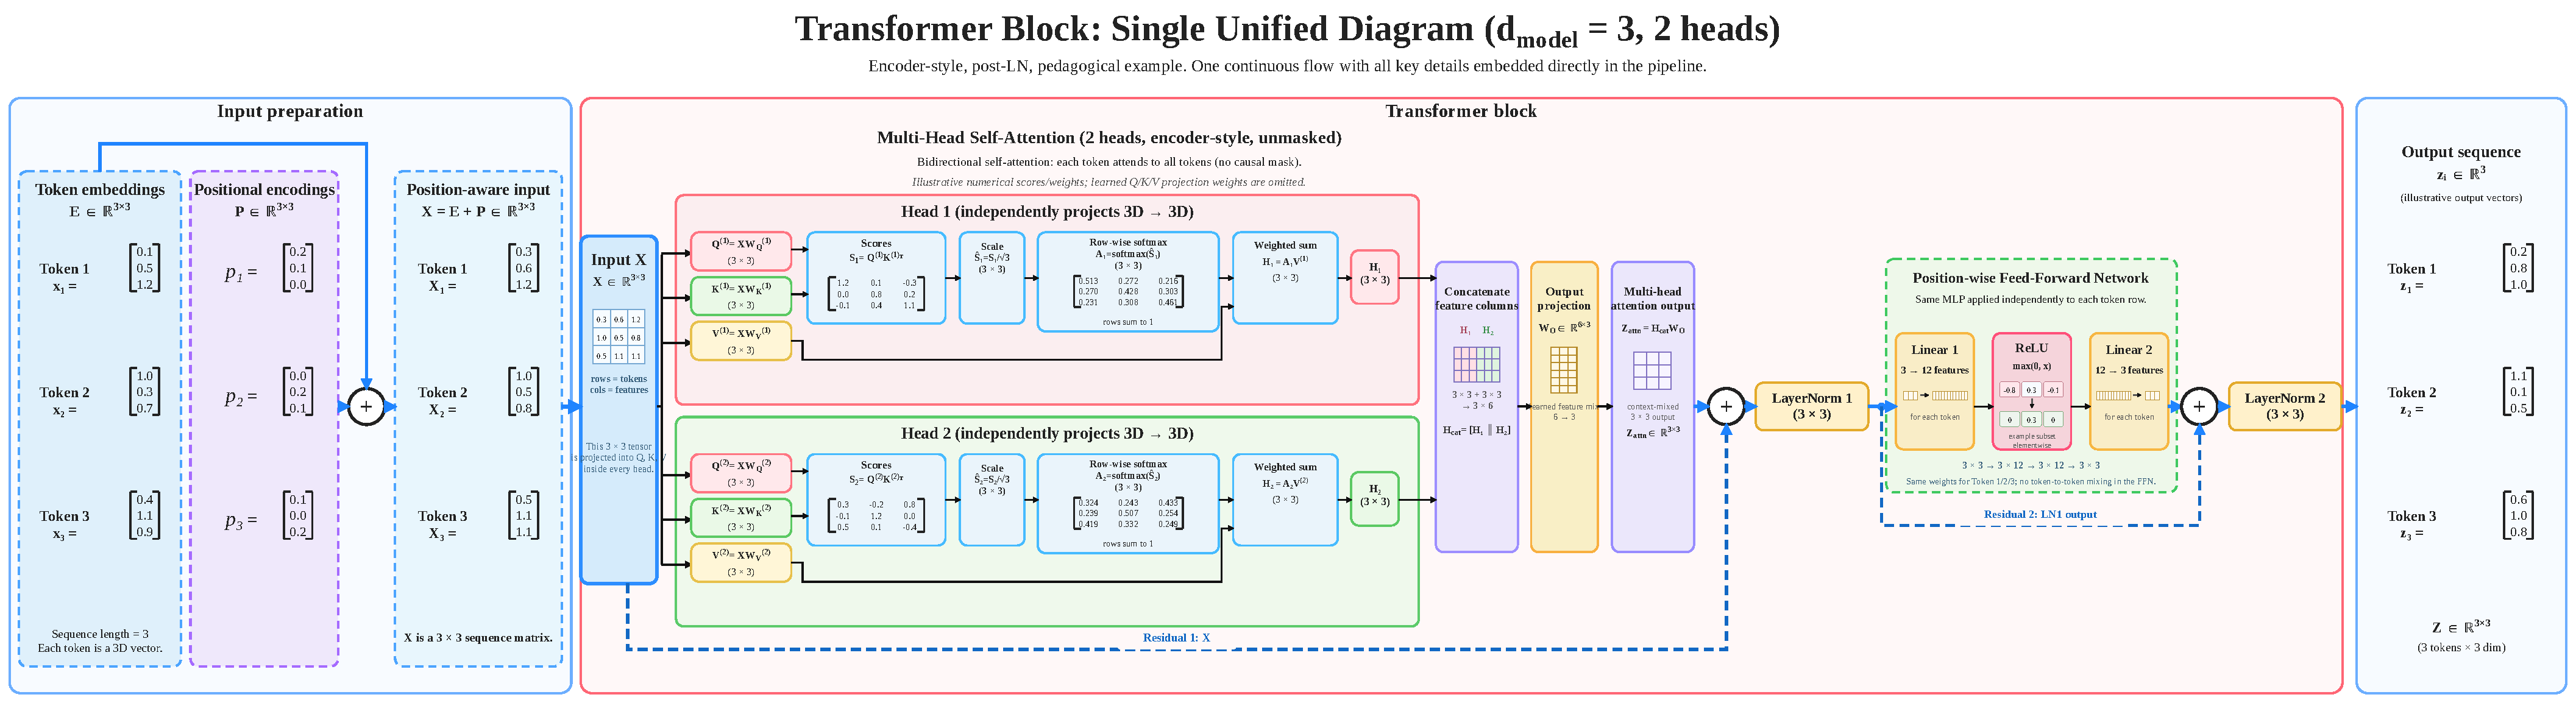
\includegraphics[width=\textwidth]{figures/transformer_format_fixed_v7.pdf}
This is the table worth knowing for research interviews.

\begin{center}
\small
\begin{longtable}{@{}L{.24\linewidth}L{.68\linewidth}@{}}
\toprule
\textbf{Method} & \textbf{Main inductive bias / assumption} \\
\midrule
\endhead
Tokenisation & useful linguistic structure can be represented by chosen discrete units \\
Sinusoidal positions & sequence position has smooth multiscale structure \\
Relative positions & interaction depends importantly on displacement \\
RoPE & query--key similarity should incorporate relative displacement geometrically \\
Causal attention & information flows past $\rightarrow$ future \\
Cross-attention & one representation should selectively retrieve information from another \\
Transformer & arbitrary pairwise content-dependent interactions are useful \\
RNN & history can be compressed into a fixed state \\
S4 & history can be represented through structured dynamical evolution \\
Transformer-XL & earlier hidden states should remain explicitly reusable \\
Griffin & nearby information benefits from attention; long-term information can be recurrently compressed \\
Perceiver & large inputs can be compressed through a latent bottleneck \\
MoE & different inputs benefit from specialised parameter subsets \\
LoRA & useful adaptation lies in a low-dimensional parameter-update space \\
Pretraining & predicting data structure produces reusable representations \\
SFT & desired behaviour can be learned by imitation \\
RLHF & comparative human preference provides a useful behavioural signal \\
FlashAttention & \textbf{no new modelling bias}; implementation optimisation \\
Decoding & \textbf{no training bias}; controls how model probabilities become outputs \\
\bottomrule
\end{longtable}
\end{center}


This is a useful classification when reading papers.

\begin{center}
\small
\caption{Useful classification when reading papers}
\begin{tabularx}{.92\linewidth}{@{}L{.31\linewidth}Y@{}}
\toprule
\textbf{Design layer} & \textbf{Examples} \\
\midrule
Input representation & tokenisation \\
Positional representation & sinusoidal, relative, RoPE \\
Information-flow constraint & causal masking \\
Information source & cross-attention \\
Sequence architecture & Transformer, RNN, S4, Griffin, Transformer-XL \\
Bottleneck architecture & Perceiver \\
Hardware algorithm & FlashAttention \\
Capacity scaling & scaling laws, MoE \\
Training objective/stage & pretraining, SFT, RLHF \\
Parameter adaptation & LoRA \\
Inference policy & temperature, top-$k$, top-$p$, beam search \\
\bottomrule
\end{tabularx}
\end{center}

This taxonomy prevents a lot of category errors.

\begin{calloutexample}
``Is FlashAttention an alternative to causal attention?'' No: causal attention can be executed with FlashAttention.

``Is LoRA an alternative to Transformer?'' No: LoRA can fine-tune a Transformer.

``Is RoPE an alternative to FlashAttention?'' No: one supplies positional structure; the other makes computation efficient.

``Is MoE an alternative to scaling laws?'' No: scaling laws describe empirical behaviour; MoE is one architecture for increasing capacity efficiently.
\end{calloutexample}


Suppose you want to build an LLM capable of reading extremely long scientific papers.
You immediately have many degrees of freedom.

\begin{figure}[htbp]
\centering
\begin{tikzpicture}[node distance=6.5mm]
\node[flow] (data) {DATA\\How much? Quality? Domains?};
\node[flow,below=of data] (tok) {TOKENISER\\32k? 100k? byte fallback?};
\node[flow,below=of tok] (pos) {POSITION\\RoPE? relative? context extension?};
\node[flow,below=of pos] (arch) {ARCHITECTURE\\Transformer? XL? S4-like? Griffin-like?};
\node[flow,below=of arch] (att) {ATTENTION\\global? local? causal? FlashAttention?};
\node[flow,below=of att] (cap) {CAPACITY\\dense? MoE? how many experts?};
\node[flow,below=of cap] (train) {TRAINING\\parameters? tokens? compute balance?};
\node[flow,below=of train] (adapt) {ADAPTATION\\full fine-tune? LoRA? preference training?};
\node[yesbox,below=of adapt] (infer) {INFERENCE\\temperature? top-$p$? context?};
\draw[arr] (data)--(tok);\draw[arr] (tok)--(pos);\draw[arr] (pos)--(arch);\draw[arr] (arch)--(att);\draw[arr] (att)--(cap);\draw[arr] (cap)--(train);\draw[arr] (train)--(adapt);\draw[arr] (adapt)--(infer);
\end{tikzpicture}
\caption{Research optionality is layered: each design decision changes a different part of the system and therefore a different trade-off.}
\label{fig:modern-research-project-optionality}
\end{figure}

This is what \textbf{optionality in system design} actually looks like.
Research generally isn't ``which algorithm is best?''
It is:

\begin{quote}
Which assumptions and resource trade-offs fit this problem?
\end{quote}

\begin{calloutdegreeofexperiment}
For a long-context LLM, vary data/tokeniser, positional method, explicit versus compressed memory, local/global attention structure, kernel implementation, total versus active capacity, parameter/data/compute allocation, adaptation strategy and decoding policy.
Ablate one design layer at a time where possible so architectural and systems effects are not conflated.
\end{calloutdegreeofexperiment}

\section{Final compression}
\label{sec:modern-final-compression}
If you remember only the core distinctions:

\begin{enumerate}
\item \textbf{Tokenisation} chooses the discrete units the model sees.
\item \textbf{Positional methods} tell a permutation-insensitive Transformer about sequence order.
\item \textbf{Sinusoidal} gives structured coordinates; \textbf{relative position} directly represents distance; \textbf{RoPE} turns position into rotations so relative displacement appears naturally in $QK^\top$.
\item \textbf{Causal attention} controls \textit{which tokens may interact}; \textbf{cross-attention} controls \textit{where K/V come from}; \textbf{FlashAttention} controls \textit{how the same computation runs efficiently}.
\item \textbf{RNNs} compress history into state; \textbf{Transformers} keep explicit content-addressable history; \textbf{S4} treats sequence processing as structured state-space dynamics.
\item \textbf{Transformer-XL} adds reusable segment memory; \textbf{Griffin} combines recurrent long-term memory with local attention; \textbf{Perceiver} compresses huge inputs into a small latent workspace.
\item \textbf{Scaling laws} describe predictable empirical relationships between loss, data, parameters and compute.
\textbf{Chinchilla} emphasised that model size and training data must be balanced.
\item \textbf{MoE} separates \textit{total parameter capacity} from \textit{parameters activated for one token}.
\item \textbf{Pretraining} builds general capability; \textbf{fine-tuning} changes behaviour for a narrower distribution; \textbf{LoRA} makes that adaptation low-rank and cheap.
\item \textbf{RLHF} introduces human preference information after pretraining/SFT.
\item \textbf{Decoding} happens after the neural network has produced its probabilities and decides how those probabilities become actual text.
\end{enumerate}

\section{Research evolution: how should sequence information move?}
\label{sec:transformers-evolution}
\begin{center}
\small
\begin{tabularx}{.97\linewidth}{@{}L{.18\linewidth}L{.21\linewidth}YY@{}}
\toprule
\textbf{Step} & \textbf{What changed} & \textbf{Problem targeted} & \textbf{New trade-off} \\
\midrule
RNN & Compress history into recurrent state & Sequence dependence & Sequential bottleneck / long-memory difficulty \\
Attention on RNNs & Directly retrieve useful past states & One-state bottleneck & Added pairwise matching cost \\
Transformer & Make attention the main communication mechanism & Parallel training and direct long-range routes & Dense $N^2$ interaction cost \\
Efficient attention / KV variants & Restrict or share interaction structure & Long-context/serving cost & Extra architectural bias \\
SSM branch & Compress long history into evolving state & Linear-time long sequences & Less explicit all-pairs interaction \\
\bottomrule
\end{tabularx}
\end{center}

\begin{calloutbias}
If useful relationships between sequence elements depend on content, attention can dynamically route information; if most useful interaction is local or compressible into state, unrestricted dense attention may spend unnecessary compute.
\end{calloutbias}

\begin{calloutdegreeofexperiment}
Vary depth, representation width, head count/dimension, attention pattern, positional mechanism, context length, MLP expansion, normalisation/residual placement and key/value sharing.
\end{calloutdegreeofexperiment}

\section{Walkthrough}
Connecting everything: one token through an imaginary modern LLM}
\label{sec:modern-one-token-through-system}
Let's now run a single token through an imaginary modern LLM.
You type:
\begin{quote}
Why is the sky blue?
\end{quote}

\paragraph{Stage A --- tokenisation.}
Raw characters become token pieces and then integer IDs.
The tokenizer determines the atomic units.

\paragraph{Stage B --- embeddings.}
Each ID becomes a vector
\[
x_i\in\mathbb R^{N_{\text{representation dims}}}.
\]

\paragraph{Stage C --- positional information.}
Suppose the model uses RoPE.
Queries and keys are rotated according to their positions.

\paragraph{Stage D --- causal attention.}
For every token, calculate scaled query--key compatibility, then apply the causal mask so future positions are forbidden.

\paragraph{Stage E --- efficient execution.}
The implementation may use FlashAttention: the same mathematical attention is tiled to reduce memory traffic.

\paragraph{Stage F --- next-token probabilities.}
The final hidden state is projected to vocabulary logits, then softmax produces $P(\text{next token})$.

\paragraph{Stage G --- decoding.}
Perhaps temperature and top-$p$ are applied, a token is sampled, appended, and the process repeats.

\begin{figure}[htbp]
\centering
\resizebox{.97\linewidth}{!}{%
\begin{tikzpicture}[node distance=6mm and 7mm]
\node[flow] (prompt) {Prompt};
\node[flow,right=of prompt] (tok) {Tokenise};
\node[flow,right=of tok] (emb) {Embedding};
\node[flow,right=of emb] (rope) {RoPE};
\node[flow,right=of rope] (att) {Causal attention\\via FlashAttention};
\node[flow,right=of att] (logit) {Vocabulary\\logits};
\node[flow,right=of logit] (dec) {Temperature\\+ top-$p$};
\node[yesbox,right=of dec] (next) {Next token};
\draw[arr] (prompt)--(tok);\draw[arr] (tok)--(emb);\draw[arr] (emb)--(rope);\draw[arr] (rope)--(att);\draw[arr] (att)--(logit);\draw[arr] (logit)--(dec);\draw[arr] (dec)--(next);
\draw[arr,rounded corners] (next.south)--++(0,-.7)--([yshift=-.7cm]prompt.south)--(prompt.south);
\end{tikzpicture}}
\caption{One autoregressive generation loop with the major mechanisms from this chapter attached to their actual place in the data flow.}
\label{fig:modern-one-token-loop}
\end{figure}



























\chapter{Architectures: Graph Neural Networks}
\label{sec:arch-gnn}

A graph neural network (GNN) updates an entity by combining its current representation with information from entities connected to it.
The architecture therefore makes a structural choice before learning begins: \emph{which pairs of entities are allowed to exchange information?}
For a CNN that relation is a fixed local image grid; for a Transformer it is commonly a dense or masked attention pattern; for a GNN it is supplied or constructed as a graph.

\begin{figure}[htbp]
\centering
\begin{tikzpicture}[scale=0.95, every node/.style={font=\small}]
  % CNN
  \node[font=\bfseries] at (-4.2,2.05) {CNN};
  \foreach \x in {-5.0,-4.2,-3.4} {
    \foreach \y in {0.2,1.0,1.8} {
      \node[circle,draw,inner sep=1.6pt] (c\x\y) at (\x,\y) {};
    }
  }
  \foreach \x in {-5.0,-4.2,-3.4} {
    \draw (\x,0.2)--(\x,1.0)--(\x,1.8);
  }
  \foreach \y in {0.2,1.0,1.8} {
    \draw (-5.0,\y)--(-4.2,\y)--(-3.4,\y);
  }
  \node[align=center] at (-4.2,-0.45) {fixed local\\grid neighbours};

  % GNN
  \node[font=\bfseries] at (0,2.05) {GNN};
  \node[circle,draw,minimum size=6mm] (g1) at (-0.9,1.15) {};
  \node[circle,draw,minimum size=6mm] (g2) at (0.2,1.65) {};
  \node[circle,draw,minimum size=6mm] (g3) at (1.0,0.8) {};
  \node[circle,draw,minimum size=6mm] (g4) at (-0.2,0.35) {};
  \node[circle,draw,minimum size=6mm] (g5) at (-1.15,0.15) {};
  \draw (g1)--(g2)--(g3)--(g4)--(g1);
  \draw (g4)--(g5)--(g1);
  \node[align=center] at (0,-0.45) {supplied or constructed\\graph neighbours};

  % Transformer
  \node[font=\bfseries] at (4.2,2.05) {Transformer};
  \foreach \i/\x in {1/3.1,2/3.8,3/4.5,4/5.2} {
    \node[circle,draw,minimum size=6mm] (t\i) at (\x,0.95) {};
  }
  \foreach \i in {1,...,4} {
    \foreach \j in {1,...,4} {
      \ifnum\i<\j\relax\draw[opacity=0.55] (t\i)--(t\j);\fi
    }
  }
  \node[align=center] at (4.2,-0.45) {potentially dense\\learned interaction};
\end{tikzpicture}
\caption{Three interaction biases. CNNs hard-code a regular local neighbourhood, GNNs communicate along graph edges, and dense self-attention can make every element a candidate interaction. The difference is primarily an information-routing choice.}
\label{fig:gnn-cnn-transformer}
\end{figure}

\begin{calloutintuition}
A GNN is a neural network whose communication routes are a graph.
\end{calloutintuition}

\section{Graph representation: entities, relations and features}
A graph contains a set of nodes $\mathcal V$ and edges $\mathcal E$.
For learning, nodes usually carry features $x_i$, edges may carry features $e_{ij}$, and the complete graph may carry global context $u$.
The adjacency structure says which node pairs are connected; unlike an image grid, the number and arrangement of neighbours can vary from node to node.

\[
\underbrace{G}_{\text{one graph}}
=
\left(
\underbrace{\{x_i\}_{i\in\mathcal V}}_{\text{node information}},
\underbrace{\{(i,j,e_{ij})\}_{(i,j)\in\mathcal E}}_{\text{relations / edge information}},
\underbrace{u}_{\text{optional graph context}}
\right).
\]

An edge may mean a chemical bond, road connection, social interaction, mesh adjacency, physical contact or a relation in a knowledge graph.
That meaning matters because the graph itself is part of the model's prior structure rather than merely a storage format.
Directed graphs distinguish $i\rightarrow j$ from $j\rightarrow i$; heterogeneous graphs may additionally distinguish node and edge types, so a relation such as \texttt{author-of} need not share parameters with \texttt{cites}.

\begin{figure}[htbp]
\centering
\begin{tikzpicture}[scale=0.95, every node/.style={font=\small}]
  \node[circle,draw,minimum size=8mm] (a) at (-2.2,0.6) {$x_1$};
  \node[circle,draw,minimum size=8mm] (b) at (0,1.35) {$x_2$};
  \node[circle,draw,minimum size=8mm] (c) at (2.1,0.55) {$x_3$};
  \node[circle,draw,minimum size=8mm] (d) at (0,-0.65) {$x_4$};
  \draw[->] (a)--node[above] {$e_{12}$}(b);
  \draw[->] (b)--node[above] {$e_{23}$}(c);
  \draw[->] (c)--node[below right] {$e_{34}$}(d);
  \draw[->] (d)--node[below left] {$e_{41}$}(a);
  \draw[->] (a)--node[below] {$e_{14}$}(d);
  \node[draw,rounded corners,align=left] at (5.0,0.35) {
    node feature $x_i$\\
    edge feature $e_{ij}$\\
    graph context $u$
  };
\end{tikzpicture}
\caption{The graph gives both values and routing structure. Node features describe entities; edge features can describe the relation through which information travels.}
\label{fig:gnn-graph-representation}
\end{figure}

\subsection{Graph construction.}
Sometimes the graph is observed directly, such as bonds in a molecule or links in a road network.
Sometimes it is a modelling choice: connect spatial points within a radius, connect each point to its $N_{\text{neighbours}}$ nearest neighbours, or learn an affinity from representations.
This distinction is important because changing the graph changes which information can meet before any neural parameter changes.

\section{Message passing: the core operation}
Most classical GNNs can be understood as repeated \textbf{message passing}.
For node $i$, each neighbour $j$ creates a message, the incoming messages are aggregated, and the result updates the node representation:

\[
\begin{aligned}
\underbrace{m_i^{(\ell)}}_{\text{incoming neighbourhood information}}
&=
\operatorname{Aggregate}_{j\in\mathcal N(i)}
\left[
\operatorname{Message}_{\theta}
\left(
\underbrace{h_i^{(\ell)}}_{\text{receiver}},
\underbrace{h_j^{(\ell)}}_{\text{sender}},
\underbrace{e_{ij}}_{\text{relation}}
\right)
\right],\\[1mm]
\underbrace{h_i^{(\ell+1)}}_{\text{new node representation}}
&=
\operatorname{Update}_{\theta}
\left(
\underbrace{h_i^{(\ell)}}_{\text{current node state}},
\underbrace{m_i^{(\ell)}}_{\text{neighbour summary}}
\right).
\end{aligned}
\]

The graph chooses the candidate senders $\mathcal N(i)$; the neural functions decide what information those senders contribute and how the receiver changes.
A self-loop or explicit residual path lets the node preserve its own information instead of replacing it with a pure neighbourhood summary.

\begin{figure}[htbp]
\centering
\begin{tikzpicture}[scale=0.96, every node/.style={font=\small}]
  \node[circle,draw,minimum size=9mm] (n1) at (-4,1.1) {$h_1$};
  \node[circle,draw,minimum size=9mm] (n2) at (-4,0) {$h_2$};
  \node[circle,draw,minimum size=9mm] (n3) at (-4,-1.1) {$h_3$};
  \node[draw,rounded corners,minimum width=2.1cm,minimum height=1.0cm,align=center] (msg) at (-1.6,0) {message\\function};
  \node[draw,rounded corners,minimum width=2.1cm,minimum height=1.0cm,align=center] (agg) at (1.1,0) {permutation-safe\\aggregate};
  \node[draw,rounded corners,minimum width=2.1cm,minimum height=1.0cm,align=center] (upd) at (3.8,0) {update\\node $i$};
  \draw[->] (n1)--(msg);
  \draw[->] (n2)--(msg);
  \draw[->] (n3)--(msg);
  \draw[->] (msg)--node[above] {messages}(agg);
  \draw[->] (agg)--node[above] {neighbour summary}(upd);
  \node[circle,draw,minimum size=9mm] (self) at (3.8,-1.55) {$h_i$};
  \draw[->] (self)--(upd);
\end{tikzpicture}
\caption{One message-passing layer. Neighbour states are transformed into messages, combined without depending on arbitrary neighbour order, then merged with the receiver state.}
\label{fig:gnn-message-passing}
\end{figure}

\subsection{The main research split.}
Papers that appear to propose very different GNNs often modify only one of four places: the graph, the message, the aggregation rule, or the update/readout.
This decomposition is more useful than memorising model names because it identifies the actual design change.

\section{Depth is graph distance}
One message-passing layer lets a node use one-hop neighbours.
Two layers allow information from nodes two edges away to arrive through an intermediate node; after $L$ layers, a node can usually depend on its $L$-hop neighbourhood.
Depth therefore controls both neural transformation and communication distance.

\begin{figure}[htbp]
\centering
\begin{tikzpicture}[scale=0.92, every node/.style={font=\small}]
  \node[circle,draw,thick,minimum size=8mm] (c) at (0,0) {$i$};
  \foreach \a/\name in {0/a,60/b,120/c1,180/d,240/e,300/f} {
    \node[circle,draw,minimum size=7mm] (\name) at (\a:1.35) {};
    \draw (c)--(\name);
  }
  \foreach \parent/\ang/\child in {a/0/a2,b/60/b2,c1/120/c2,d/180/d2,e/240/e2,f/300/f2} {
    \node[circle,draw,minimum size=6mm] (\child) at (\ang:2.55) {};
    \draw (\parent)--(\child);
  }
  \draw[dashed] (0,0) circle (1.75);
  \draw[dotted] (0,0) circle (2.9);
  \node[align=left] at (4.4,1.1) {1 layer: one-hop evidence};
  \node[align=left] at (4.4,0.2) {2 layers: two-hop evidence};
  \node[align=left] at (4.4,-0.7) {more depth: wider graph receptive field};
\end{tikzpicture}
\caption{Graph depth expands a node's receptive field by graph distance rather than Euclidean distance or sequence position.}
\label{fig:gnn-receptive-field}
\end{figure}

This is analogous to CNN receptive fields in Section~12, but graph distance follows connectivity rather than pixels.
A long graph path can separate physically close nodes, while one edge can connect geometrically distant entities.

\begin{calloutintuition}
GNN depth is communication distance: $L$ message-passing layers expose roughly an $L$-hop neighbourhood.
\end{calloutintuition}

\section{Permutation symmetry: node numbers should not matter}
Node IDs normally have no semantic ordering.
Renumbering the same graph should therefore renumber node-level outputs consistently, while a graph-level prediction should remain unchanged.
If $P$ is a permutation matrix, a node-level GNN should satisfy the equivariance relation

\[
\underbrace{f(PX,\,PAP^\top)}_{\text{same graph with reordered node IDs}}
=
\underbrace{P f(X,A)}_{\text{same node outputs, reordered}}.
\]

For a graph-level readout $r$, the corresponding requirement is invariance:

\[
\underbrace{r(PH)}_{\text{reordered nodes}}
=
\underbrace{r(H)}_{\text{same graph prediction}}.
\]

Sum, mean and max are useful aggregation operations because their result does not depend on the order in which neighbours are presented.
Concatenating neighbours in arbitrary storage order would instead make node numbering part of the function.

\subsection{Inductive bias.}
If node identity is arbitrary but relations are meaningful, permutation equivariance lets one learned local rule operate anywhere in the graph.
If absolute node identity itself carries information, that information must be represented explicitly rather than accidentally through array position.

\section{GCN: normalised neighbour mixing}
A Graph Convolutional Network (GCN) makes message passing deliberately simple: add self-connections, mix neighbouring features with degree normalisation, then apply a learned feature transform.
A common layer is

\[
\begin{aligned}
\widetilde A&=A+I,\\
\underbrace{H^{(\ell+1)}}_{\text{updated node representations}}
&=
\phi\!\left(
\underbrace{\widetilde D^{-1/2}\widetilde A\widetilde D^{-1/2}}_{\text{normalised graph mixing}}
\underbrace{H^{(\ell)}\theta_{\text{features}}^{(\ell)}}_{\text{learned feature transform}}
\right).
\end{aligned}
\]

Degree normalisation prevents high-degree nodes from automatically producing proportionally larger summed activations merely because they have more neighbours.
The layer is therefore a learned feature transform wrapped around a graph smoothing operation.
That bias is useful when connected nodes should share information, but repeated smoothing becomes a failure mode when neighbours should remain distinct.

\begin{calloutintuition}
GCN = learn features while repeatedly smoothing them across graph edges.
\end{calloutintuition}

\section{GraphSAGE: sample and aggregate}
Full-neighbour aggregation becomes expensive when high-degree nodes connect to thousands or millions of neighbours.
GraphSAGE makes the neighbourhood itself part of the approximation: sample a bounded set of neighbours, aggregate their states, and combine the result with the target node.

\[
\begin{aligned}
\underbrace{\widehat{\mathcal N}(i)}_{\text{sampled neighbours}}
&\subseteq
\underbrace{\mathcal N(i)}_{\text{all neighbours}},\\[-1mm]
&\text{bounded work}
\quad\leftrightarrow\quad
\text{incomplete / noisier neighbourhood evidence}.
\end{aligned}
\]

GraphSAGE is also associated with \textbf{inductive} use: the model learns an aggregation rule from features rather than storing only one learned embedding per training node, so it can process previously unseen nodes when their features and neighbourhood are available.
This does not mean every GraphSAGE setup generalises automatically; the new graph must still resemble the training regime in the ways the learned rule relies on.

\begin{figure}[htbp]
\centering
\begin{tikzpicture}[scale=0.9, every node/.style={font=\small}]
  \node[font=\bfseries] at (-3.3,2.0) {Full neighbourhood};
  \node[circle,draw,thick,minimum size=8mm] (f0) at (-3.3,0.7) {$i$};
  \foreach \a/\k in {0/1,45/2,90/3,135/4,180/5,225/6,270/7,315/8} {
    \node[circle,draw,minimum size=5mm] (f\k) at ($(-3.3,0.7)+(\a:1.1)$) {};
    \draw (f0)--(f\k);
  }
  \node[font=\bfseries] at (3.1,2.0) {Sampled neighbourhood};
  \node[circle,draw,thick,minimum size=8mm] (s0) at (3.1,0.7) {$i$};
  \foreach \a/\k in {20/1,105/2,210/3,300/4} {
    \node[circle,draw,minimum size=5mm] (s\k) at ($(3.1,0.7)+(\a:1.1)$) {};
    \draw[thick] (s0)--(s\k);
  }
  \node at (0,-1.0) {$\text{less work} \;\leftrightarrow\; \text{less complete local evidence}$};
\end{tikzpicture}
\caption{Neighbour sampling bounds compute and memory, but the sampled subgraph is an estimator of the full neighbourhood rather than the full neighbourhood itself.}
\label{fig:gnn-neighbour-sampling}
\end{figure}

\section{GAT: learn which neighbours matter}
A Graph Attention Network (GAT) keeps graph edges as the set of allowed interactions but learns how strongly each permitted neighbour contributes.
For node $i$,

\[
\begin{aligned}
\underbrace{\alpha_{ij}}_{\text{importance of neighbour }j}
&=
\operatorname{softmax}_{j\in\mathcal N(i)}
\left(
\underbrace{\operatorname{score}_{\theta}(h_i,h_j,e_{ij})}_{\text{content / relation compatibility}}
\right),\\[1mm]
\underbrace{h_i'}_{\text{updated node}}
&=
\phi\!\left(
\sum_{j\in\mathcal N(i)}
\alpha_{ij}\,\theta_{\text{value}}h_j
\right).
\end{aligned}
\]

This is conceptually close to attention in Section~13.1, but the graph commonly supplies a sparse mask: only connected nodes compete for attention weight.
The graph therefore says \emph{who may speak}; attention decides \emph{who matters for this update}.
Multi-head graph attention adds the same broad optionality as multi-head Transformer attention: different heads can represent different relation patterns, at additional memory and compute cost.

\begin{figure}[htbp]
\centering
\begin{tikzpicture}[scale=1.0, every node/.style={font=\small}]
  \node[circle,draw,thick,minimum size=9mm] (i) at (0,0) {$i$};
  \node[circle,draw,minimum size=8mm] (a) at (-2,1.15) {$j_1$};
  \node[circle,draw,minimum size=8mm] (b) at (-2,0) {$j_2$};
  \node[circle,draw,minimum size=8mm] (c) at (-2,-1.15) {$j_3$};
  \draw[->,line width=1.8pt] (a)--node[above,sloped] {$\alpha_{i1}$}(i);
  \draw[->,line width=0.5pt] (b)--node[above,sloped] {$\alpha_{i2}$}(i);
  \draw[->,line width=1.1pt] (c)--node[below,sloped] {$\alpha_{i3}$}(i);
  \node[align=left] at (4.2,0.55) {same permitted edges};
  \node[align=left] at (4.2,-0.15) {different learned weights};
\end{tikzpicture}
\caption{Graph attention learns importance inside the allowed neighbourhood. Edge thickness represents a larger or smaller learned contribution, not a change in connectivity.}
\label{fig:gnn-gat}
\end{figure}

\section{GCN, GraphSAGE and GAT are choices inside one mechanism}
The model names are less important than the message-passing choices they instantiate.

\begin{table}[htbp]
\centering
\small
\begin{tabular}{p{0.14\textwidth}p{0.21\textwidth}p{0.23\textwidth}p{0.26\textwidth}}
\toprule
Method & Neighbour rule & What it buys & Main cost / assumption \\
\midrule
GCN & normalised mixing over graph neighbours & simple, efficient local smoothing & connected nodes should benefit from mixing; full neighbourhood may be costly \\
GraphSAGE & sample neighbours, then aggregate & bounded neighbourhood work; natural inductive use & sampling variance and missed neighbours \\
GAT & learned attention over allowed neighbours & content-dependent neighbour importance & extra scoring work; edges still constrain candidate interactions \\
General MPNN & learned message + aggregation + update & flexible node/edge interaction design & more capacity and more ways to overfit or spend compute \\
\bottomrule
\end{tabular}
\caption{Several common GNN families differ mainly in how they construct and weight messages, not in the broad data flow.}
\label{tab:gnn-families}
\end{table}

\section{MPNN: the general abstraction}
A Message Passing Neural Network (MPNN) treats the message function itself as learnable and may use edge features explicitly.
For molecular graphs, for example, the message from atom $j$ to atom $i$ can depend on the sender representation, receiver representation and bond type rather than only a scalar adjacency entry.
The same abstraction covers many architectures:

\[
\boxed{
\text{graph construction}
\rightarrow
\text{message}
\rightarrow
\text{aggregate}
\rightarrow
\text{update}
\rightarrow
\text{readout}
}
\]

When reading a GNN paper, first locate which arrow changed.
A new name can hide a small local architectural change; conversely, a change to graph construction or symmetry constraints can alter the hypothesis class substantially even if the neural block looks familiar.

\section{Expressivity: aggregation can destroy distinctions}
Permutation-safe aggregation deliberately compresses a set of neighbour states into one vector.
Compression creates collisions: two different neighbourhoods can produce the same aggregate, after which later layers cannot reconstruct which neighbourhood was present.
For example, a simple mean discards neighbour count when two multisets have the same average.

Many standard message-passing GNNs are closely related in distinguishing power to the one-dimensional Weisfeiler--Lehman (1-WL) graph-refinement procedure: some non-isomorphic graph structures remain indistinguishable regardless of training.
The practical consequence is not that message passing is weak in general; it is that architecture-level symmetry and aggregation choices bound what structure can ever become visible to the predictor.
Higher-order, subgraph, positional-encoding and graph-Transformer methods add information specifically to break some of these collisions, usually at increased compute or reduced symmetry simplicity.

\begin{calloutintuition}
Aggregation buys permutation symmetry by throwing information away; expressivity depends on what survives that compression.
\end{calloutintuition}

\section{Prediction level: node, edge or whole graph}
The same message-passing backbone can support different prediction targets.
A node task reads one or more node states; an edge task scores a pair of node states; a graph task first compresses all node states into one graph representation.

\begin{figure}[htbp]
\centering
\begin{tikzpicture}[scale=0.92, every node/.style={font=\small}]
  \node[circle,draw] (a) at (-4,0.7) {};
  \node[circle,draw] (b) at (-3.2,1.25) {};
  \node[circle,draw] (c) at (-2.5,0.45) {};
  \node[circle,draw] (d) at (-3.35,-0.25) {};
  \draw (a)--(b)--(c)--(d)--(a);
  \draw (b)--(d);
  \node at (-3.25,-1.0) {shared GNN states};

  \draw[->] (-2.0,0.5)--(-0.9,1.55);
  \node[draw,rounded corners,align=center] at (0.2,1.55) {node\\prediction};

  \draw[->] (-2.0,0.3)--(-0.9,0.25);
  \node[draw,rounded corners,align=center] at (0.2,0.25) {edge / link\\prediction};

  \draw[->] (-2.0,0.05)--(-0.9,-1.05);
  \node[draw,rounded corners,align=center] at (0.2,-1.05) {pool nodes\\$\rightarrow$ graph prediction};

  \node[align=left] at (4.1,1.55) {Which node is fraudulent?};
  \node[align=left] at (4.1,0.25) {Will these nodes connect?};
  \node[align=left] at (4.1,-1.05) {What property has this molecule?};
\end{tikzpicture}
\caption{Prediction level changes the readout, not necessarily the message-passing backbone.}
\label{fig:gnn-prediction-levels}
\end{figure}

\subsection{Link prediction.}
A link score often uses a dot product, bilinear score or small neural function of two node states.
Negative examples are usually far more numerous than observed positive edges, so the negative-sampling policy becomes part of the training problem rather than a harmless implementation detail.

\section{Pooling: many nodes to one graph state}
Graph-level prediction needs a permutation-invariant readout.
Common choices expose different information:

\begin{table}[htbp]
\centering
\small
\begin{tabular}{p{0.18\textwidth}p{0.32\textwidth}p{0.38\textwidth}}
\toprule
Readout & Preserves / emphasises & Main consequence \\
\midrule
Sum & accumulated evidence and graph size & can represent counts; magnitude grows with node count \\
Mean & average node evidence & normalises graph size but can erase count information \\
Max & strongest feature presence & detects whether a strong local signal exists; ignores multiplicity \\
Learned pooling & task-dependent selection / coarsening & more expressive compression but adds parameters and possible instability \\
\bottomrule
\end{tabular}
\caption{Pooling is an information-compression choice. No readout is universally best because each preserves different graph statistics.}
\label{tab:gnn-pooling}
\end{table}

Hierarchical pooling instead produces progressively coarser graphs, analogous to reducing spatial resolution in a CNN.
The useful question is what information may safely disappear when many local states become one global state.

\section{The central inductive bias}
A GNN assumes that the supplied relation structure identifies useful routes for sharing information and that some update rule can be reused across many nodes or edges.
This can give strong data efficiency when the graph matches the mechanism generating the target.
It can also hard-code the wrong interactions when the supplied topology is noisy, missing, adversarial or simply unrelated to the prediction target.

\begin{table}[htbp]
\centering
\small
\begin{tabular}{p{0.16\textwidth}p{0.34\textwidth}p{0.38\textwidth}}
\toprule
Architecture & Structural preference / assumption & Useful regime \\
\midrule
CNN & nearby grid positions contain reusable local patterns & images and other regular spatial grids \\
GNN & connected entities should exchange information through reusable relation-aware rules & molecules, networks, meshes, relational data \\
Transformer & useful interactions can be selected largely from content, often among many candidate pairs & sequences / sets with flexible long-range interaction \\
\bottomrule
\end{tabular}
\caption{CNNs, GNNs and Transformers differ mainly in how strongly the architecture constrains the interaction graph before learning.}
\label{tab:gnn-inductive-bias}
\end{table}

\subsection{Inductive bias.}
If the known graph is a good approximation to the task's dependency structure, sparse message passing spends capacity on plausible interactions and shares parameters efficiently.
If useful dependencies routinely cross missing edges, the same sparsity can prevent information from meeting until many layers later or prevent it entirely.

\section{GNN versus Transformer: supplied topology or learned topology}
The sharpest comparison is not ``graph data versus text data''; both architectures can process many data types.
The sharper distinction is the communication prior.

\[
\underbrace{\text{GNN}}_{\text{topology constrains interaction}}
\qquad\longleftrightarrow\qquad
\underbrace{\text{Transformer}}_{\text{content can select among broad candidate interactions}}.
\]

A GAT already mixes the ideas: the graph restricts the candidate set, then attention chooses relative importance inside that set.
A graph Transformer can relax the restriction further by allowing long-range or dense attention while injecting graph distance, edge type or other structural information into the attention calculation.
The trade-off is predictable: relaxing graph sparsity can improve access to distant evidence but moves compute and memory toward the all-pairs costs discussed in Section~13.1.

\begin{figure}[htbp]
\centering
\begin{tikzpicture}[scale=0.9, every node/.style={font=\small}]
  \node[font=\bfseries] at (-4.0,2.0) {Sparse message passing};
  \node[font=\bfseries] at (0,2.0) {Graph attention};
  \node[font=\bfseries] at (4.0,2.0) {Dense attention};

  \foreach \offset in {-4,0,4} {
    \node[circle,draw,minimum size=5mm] (a\offset) at (\offset-0.8,0.9) {};
    \node[circle,draw,minimum size=5mm] (b\offset) at (\offset,1.3) {};
    \node[circle,draw,minimum size=5mm] (c\offset) at (\offset+0.8,0.75) {};
    \node[circle,draw,minimum size=5mm] (d\offset) at (\offset,0.15) {};
  }
  \draw (a-4)--(b-4)--(c-4)--(d-4)--(a-4);
  \draw[line width=1.4pt] (a0)--(b0);
  \draw[line width=0.5pt] (b0)--(c0);
  \draw[line width=1.0pt] (c0)--(d0);
  \draw[line width=0.8pt] (d0)--(a0);
  \draw[opacity=0.55] (a4)--(b4)--(c4)--(d4)--(a4);
  \draw[opacity=0.55] (a4)--(c4);
  \draw[opacity=0.55] (b4)--(d4);

  \node[align=center] at (-4,-0.55) {edges decide\\possible communication};
  \node[align=center] at (0,-0.55) {edges decide possible;\\attention decides importance};
  \node[align=center] at (4,-0.55) {many / all pairs\\can interact directly};
\end{tikzpicture}
\caption{Graph attention is a useful bridge between message passing and Transformer-style routing. Relaxing the sparse graph increases optional interaction paths but usually increases cost.}
\label{fig:gnn-to-transformer}
\end{figure}

\section{Failure mode: over-smoothing}
Neighbour mixing repeatedly pulls connected representations toward each other.
With enough smoothing-dominated layers, node states in a connected region can become difficult to distinguish, even if deeper receptive fields would in principle provide more context.
This is \textbf{over-smoothing}.

\[
\underbrace{\text{more message-passing depth}}_{\text{larger receptive field}}
\quad\Rightarrow\quad
\underbrace{\text{more repeated mixing}}_{\text{representations can converge}}
\quad\Rightarrow\quad
\underbrace{\text{less node-specific information}}_{\text{harder discrimination}}.
\]

Residual connections, normalisation, gating, decoupled propagation and shallower architectures can reduce the effect, but they do not make useful depth free.
Residual connections and normalisation are developed more generally in Section~8; here they act on a graph-specific problem created by repeated neighbourhood mixing.

\begin{figure}[htbp]
\centering
\begin{tikzpicture}[scale=0.95, every node/.style={font=\small}]
  \node at (-4.7,1.4) {layer 0};
  \node at (0,1.4) {middle layers};
  \node at (4.7,1.4) {deep mixing};

  \foreach \x/\y in {-5.3/0.5,-4.8/-0.5,-4.2/0.85,-3.8/-0.2} {
    \node[circle,draw,minimum size=4mm] at (\x,\y) {};
  }
  \foreach \x/\y in {-0.8/0.35,-0.3/-0.25,0.25/0.55,0.75/-0.05} {
    \node[circle,draw,minimum size=4mm] at (\x,\y) {};
  }
  \foreach \x/\y in {4.45/0.15,4.65/-0.02,4.85/0.18,5.05/0.02} {
    \node[circle,draw,minimum size=4mm] at (\x,\y) {};
  }
  \draw[->] (-3.2,0.2)--(-1.4,0.2);
  \draw[->] (1.3,0.2)--(3.2,0.2);
  \node at (0,-1.0) {node representations become less separated};
\end{tikzpicture}
\caption{Over-smoothing is representation collapse under repeated neighbourhood mixing. The diagram is conceptual: actual embedding geometry depends on the graph, parameters and training.}
\label{fig:gnn-oversmoothing}
\end{figure}

\section{Failure mode: over-squashing}
Over-squashing is different.
The problem is not that nearby node states become too similar; it is that information from a rapidly growing distant neighbourhood must be compressed through fixed-width states or narrow graph cuts before reaching the target.

\begin{figure}[htbp]
\centering
\begin{tikzpicture}[scale=0.9, every node/.style={font=\small}]
  \foreach \y/\k in {1.5/1,0.9/2,0.3/3,-0.3/4,-0.9/5,-1.5/6} {
    \node[circle,draw,minimum size=5mm] (l\k) at (-4.0,\y) {};
  }
  \node[circle,draw,minimum size=6mm] (b) at (-1.0,0) {};
  \node[circle,draw,minimum size=7mm] (t) at (2.0,0) {$i$};
  \foreach \k in {1,...,6} {\draw[->] (l\k)--(b);}
  \draw[->,line width=1.5pt] (b)--(t);
  \node[align=center] at (-4,-2.1) {many distant\\signals};
  \node[align=center] at (-1,-1.1) {narrow\\cut};
  \node[align=center] at (2,-1.1) {target};
  \node[align=left] at (5.0,0.35) {many dependencies};
  \node[align=left] at (5.0,-0.35) {$\rightarrow$ fixed-size bottleneck};
\end{tikzpicture}
\caption{Over-squashing: many distant dependencies are forced through a small information bottleneck. This can occur even when node representations have not over-smoothed.}
\label{fig:gnn-oversquashing}
\end{figure}

Increasing representation width, changing graph connectivity, adding long-range edges, using global attention or improving positional/structural information can help in different regimes.
These fixes target different mechanisms, so ``make the GNN deeper'' is often the wrong response to a long-range dependency problem.

\begin{calloutintuition}
Over-smoothing makes nodes too similar; over-squashing forces too much distant information through too little channel capacity.
\end{calloutintuition}

\section{Heterophily: neighbours need not look alike}
Many successful graph benchmarks are approximately \textbf{homophilic}: connected nodes often share labels or features.
Neighbour smoothing naturally fits that regime.
Other graphs are \textbf{heterophilic}: useful edges connect different roles, classes or states, such as buyers to sellers or reactants with complementary chemical roles.
In that case, blindly averaging neighbours can erase the distinction the task needs.

The architectural response may be relation-specific parameters, signed or directional messages, separate self and neighbour channels, higher-order structure, attention, or weaker reliance on direct neighbour similarity.
The correct question is therefore not whether graph connections exist, but what statistical meaning an edge has for the target.

\subsection{Inductive bias.}
If connected nodes should have related latent states, smoothing is useful; if edges encode complementarity rather than similarity, the message function must preserve that distinction instead of averaging it away.

\section{Graph construction can itself be learned}
A graph need not be fixed input data.
For point clouds, particles or latent representations, connectivity can be built from distance or similarity:

\[
\underbrace{\text{representations / coordinates}}_{\text{candidate entities}}
\rightarrow
\underbrace{\text{kNN / radius / learned affinity}}_{\text{construct edges}}
\rightarrow
\underbrace{\text{message passing}}_{\text{use edges}}.
\]

Recomputing neighbours after each representation update makes topology dynamic, allowing the interaction graph to evolve with the learned geometry.
This adds flexibility but couples representation learning to discrete or approximate neighbour selection, increasing instability and implementation cost.
A learned dense affinity moves still closer to self-attention: the boundary between ``GNN'' and ``Transformer'' becomes architectural rather than categorical.

\section{Geometry: invariance and equivariance}
Physical graphs often contain coordinates in addition to connectivity.
A molecular energy should not normally change because the molecule is translated or rotated; a predicted force vector should rotate with the molecule rather than remain numerically fixed.
This separates \textbf{invariance} from \textbf{equivariance}:

\[
\underbrace{f(Rx+t)}_{\text{transform input geometry}}
=
\begin{cases}
\underbrace{f(x)}_{\text{invariant scalar output}}, & \text{energy-like output},\\[2mm]
\underbrace{R f(x)}_{\text{equivariant vector output}}, & \text{force / direction-like output}.
\end{cases}
\]

Here $R$ is a rotation and $t$ a translation.
Equivariant GNNs constrain messages and features so these transformation rules hold by construction or by the chosen representation, rather than asking data augmentation alone to teach them approximately.
This is a strong inductive bias: it can improve data efficiency and physical consistency when the symmetry is correct, but it becomes a restriction when the environment contains a meaningful preferred orientation or reference frame.

\begin{figure}[htbp]
\centering
\begin{tikzpicture}[scale=0.95, every node/.style={font=\small}]
  \node[circle,draw] (a) at (-4,0) {};
  \node[circle,draw] (b) at (-3,1) {};
  \node[circle,draw] (c) at (-2.2,-0.2) {};
  \draw (a)--(b)--(c)--(a);
  \draw[->,thick] (-3,0.2)--(-2.35,0.85);
  \node at (-3,-1.0) {input geometry};

  \draw[->] (-1.2,0.25)--(0.2,0.25) node[midway,above] {rotate};

  \node[circle,draw] (d) at (1.0,-0.5) {};
  \node[circle,draw] (e) at (2.2,-0.2) {};
  \node[circle,draw] (f) at (1.45,0.95) {};
  \draw (d)--(e)--(f)--(d);
  \draw[->,thick] (1.45,0.1)--(2.15,0.35);
  \node at (1.55,-1.0) {rotated geometry};

  \node[draw,rounded corners,align=center] at (5.0,0.25) {scalar unchanged\\vector rotates};
\end{tikzpicture}
\caption{Geometric inductive bias can enforce the transformation behaviour the target should have rather than learning it separately for every orientation.}
\label{fig:gnn-equivariance}
\end{figure}

\section{Graph Transformers and structural encodings}
Dense self-attention does not automatically know which token pairs are adjacent in a graph.
Graph Transformers therefore inject structural information such as edge type, shortest-path distance, Laplacian coordinates, random-walk statistics or sparse attention masks.
These mechanisms answer a graph-specific version of the positional-encoding problem in Section~13.3: nodes form a set unless structure tells the model how one node is situated relative to another.

\begin{table}[htbp]
\centering
\small
\begin{tabular}{p{0.24\textwidth}p{0.34\textwidth}p{0.32\textwidth}}
\toprule
Structural signal & What it exposes & Main cost / caveat \\
\midrule
Graph edges / edge type & direct relations & misses long-range relation unless depth or global routing supplies it \\
Shortest-path distance & graph-relative separation & all-pairs preprocessing/storage can be expensive \\
Laplacian eigenvectors & global spectral coordinates & sign/basis ambiguities; graph-specific computation \\
Random-walk features & local-to-mesoscale connectivity statistics & additional preprocessing and scale choices \\
Global attention & direct long-range communication & can move complexity toward $O(N_{\text{nodes}}^2)$ interactions \\
\bottomrule
\end{tabular}
\caption{Graph Transformers trade stronger long-range access against additional structural machinery and, in dense forms, higher interaction cost.}
\label{tab:gnn-graph-transformer-structure}
\end{table}

A hybrid model can keep local message passing for cheap high-confidence relations and add a smaller amount of global attention for long-range dependencies.
This mirrors the broader sequence-model theme in Section~13.5: explicitly addressable interaction is expensive, while compressed or sparse communication is cheaper but more restrictive.

\section{Scaling: neighbourhood expansion and irregular memory access}
For a graph with average sampled branching factor $b$, naively expanding an $L$-layer neighbourhood around one target can touch roughly

\[
\underbrace{1+b+b^2+\cdots+b^L}_{\text{candidate nodes in an expanding computation graph}}
\]

nodes before duplicate overlaps are considered.
The problem is therefore not only arithmetic FLOPs; graph workloads also perform irregular gather/scatter operations over sparse neighbours, which can have poor memory locality compared with dense matrix operations.
Large-graph training commonly responds with neighbour sampling, subgraph/minibatch sampling, graph partitioning, cached embeddings or distributed storage.
Each method changes what information is available inside one optimisation step.

\begin{table}[htbp]
\centering
\small
\begin{tabular}{p{0.20\textwidth}p{0.34\textwidth}p{0.34\textwidth}}
\toprule
Scaling choice & Benefit & New cost \\
\midrule
Neighbour sampling & bounds fan-out per target & stochastic / incomplete neighbourhood \\
Subgraph sampling & batches locally connected regions & boundary information may be absent \\
Partitioning & distributes graph storage and compute & cross-partition communication \\
Sparse kernels & avoid dense $N_{\text{nodes}}^2$ work & irregular memory access and hardware dependence \\
Cached states & avoid repeated recomputation & staleness and invalidation-like consistency questions \\
\bottomrule
\end{tabular}
\caption{Large-graph systems trade complete neighbourhood information against tractable memory, communication and throughput.}
\label{tab:gnn-scaling}
\end{table}

\begin{calloutpracticaltip}
Profile sampled nodes/edges and memory traffic, not only parameter count; a small GNN can be bottlenecked by graph expansion and sparse data movement.
\end{calloutpracticaltip}

\section{Applications: the graph must encode a useful relation}
Graph structure is valuable when the relation itself carries predictive information.
The domain name is secondary to how entities, edges and targets are constructed.

\begin{table}[htbp]
\centering
\small
\begin{tabular}{p{0.18\textwidth}p{0.25\textwidth}p{0.25\textwidth}p{0.22\textwidth}}
\toprule
Domain & Nodes & Edges & Typical target \\
\midrule
Molecules & atoms & chemical bonds / geometric neighbours & molecular property, atom state, force \\
Recommendation & users/items or entities & interactions / relations & link likelihood, ranking feature, representation \\
Knowledge graph & typed entities & typed semantic relations & missing relation / entity prediction \\
Traffic network & road segments / sensors & physical connectivity & future traffic state \\
Meshes / PDEs & mesh cells / particles & adjacency / interaction radius & field update, dynamics, physical quantity \\
\bottomrule
\end{tabular}
\caption{A useful graph representation identifies entities and relations that align with the mechanism needed for prediction.}
\label{tab:gnn-applications}
\end{table}

For recommendation, graph methods complement rather than replace the two-tower and ranking systems in Sections~18--19: graph propagation can create richer user/item representations, while retrieval and ranking still solve the large-catalogue serving problem.
For scientific ML, graph meshes and particle systems connect directly to the physical inductive-bias discussion in Section~5.9.9.

\section{How GNN ideas evolved}
The useful history is a sequence of pressures on how graph information should move rather than a list of paper names.

\begin{table}[htbp]
\centering
\small
\begin{tabular}{p{0.15\textwidth}p{0.22\textwidth}p{0.25\textwidth}p{0.22\textwidth}}
\toprule
Stage & What changed & Pressure it addressed & New trade-off \\
\midrule
Spectral graph convolution & filters defined through graph-Laplacian structure & transfer convolution ideas to irregular domains & eigenbasis/global graph dependence can complicate scaling and transfer \\
Spatial message passing & update nodes from explicit neighbours & make locality and computation directly graph-local & long-range interaction requires depth \\
GCN-style simplification & normalised neighbourhood mixing + learned feature transform & simple scalable local baseline & smoothing bias can become restrictive \\
GraphSAGE / sampling & bounded sampled neighbourhoods & very large / evolving graphs & stochastic incomplete local evidence \\
GAT & learned neighbour weights & neighbours are not equally useful & extra attention cost \\
General MPNNs & richer node/edge messages & relations carry task-specific information & larger design and optimisation space \\
Geometric / equivariant GNNs & enforce physical transformation rules & coordinates and symmetries contain known structure & stronger assumptions, specialised operations \\
Graph Transformers / hybrids & add long-range attention + structural encodings & message-passing bottlenecks and global dependencies & denser interaction and structural-encoding cost \\
\bottomrule
\end{tabular}
\caption{A compressed evolution of GNNs: each stage changes the communication rule to address a limitation, while introducing a new cost or assumption.}
\label{tab:gnn-evolution}
\end{table}

The evolution is not a replacement chain.
GCNs remain useful baselines, sampling remains necessary at scale, equivariance matters only when the task has the relevant symmetry, and global attention is wasteful when local edges already capture the dependency structure.

\section{Research optionality: what exactly can be changed?}
A GNN experiment has design freedom at several distinct layers.
Keeping these layers separate prevents category errors such as treating neighbour sampling as an alternative to attention when the two can be used together.

\begin{table}[htbp]
\centering
\small
\begin{tabular}{p{0.26\textwidth}p{0.64\textwidth}}
\toprule
Design layer & Variables \\
\midrule
Graph construction & observed edges, kNN, radius, learned edges, direction, edge pruning, dynamic recomputation \\
Node / edge representation & raw features, embeddings, relation types, coordinates, temporal features, structural encodings \\
Message function & sender-only, sender+receiver, edge-conditioned, attention-weighted, geometric/equivariant \\
Aggregation & sum, mean, max, attention, degree normalisation, multi-aggregation \\
Update & MLP, residual, gated update, recurrent state, normalisation placement \\
Depth / range & message-passing layers, skip connections, long-range edges, global tokens/attention \\
Sampling / systems & fan-out, subgraph size, partitioning, sparse kernels, cache/staleness policy \\
Pooling / readout & sum/mean/max, set attention, hierarchical pooling, task-specific graph token \\
Objective & node, edge, graph loss; contrastive/self-supervised auxiliaries; negative sampling \\
Symmetry & permutation, translation/rotation invariance, equivariance group, coordinate frame \\
\bottomrule
\end{tabular}
\caption{The GNN research space is wider than choosing between named architectures. A paper usually changes one or a few rows of this table.}
\label{tab:gnn-optionality}
\end{table}

\subsection{Degree of experiment.}
Vary graph construction, neighbourhood radius/fan-out, representation width, message function, aggregation, attention, depth, residual/normalisation placement, edge features, structural encodings, pooling, symmetry constraints, sampling strategy and prediction objective.
Compare not only task quality but also sampled edges, memory traffic, latency/throughput and behaviour under graph perturbation or distribution shift.

\section{A diagnostic for choosing a GNN}
A graph architecture is attractive when the answer to several of the following questions is ``yes'':
\begin{enumerate}
  \item \textbf{Entities:} is the input naturally a variable-sized set of entities rather than a fixed grid or sequence?
  \item \textbf{Relations:} do known or constructible relationships identify likely information dependencies?
  \item \textbf{Reuse:} should the same local interaction rule apply across many nodes or edges?
  \item \textbf{Symmetry:} should arbitrary node ordering leave the function unchanged except for corresponding node-output reordering?
  \item \textbf{Range:} can useful evidence reach its target through a practical number of graph hops, or is global routing required?
  \item \textbf{Topology quality:} are the edges reliable enough to deserve architectural privilege?
  \item \textbf{Scale:} can the required neighbourhoods be sampled, partitioned or processed sparsely within the compute/memory budget?
\end{enumerate}

If relations are weak and arbitrary pairwise interaction is important, a set/Transformer architecture may be more natural.
If the data lie on a regular grid with strong translation-local structure, convolution may encode the same useful bias more cheaply.
If the target is mostly determined by independent node features, graph propagation can add cost and noise without buying useful information.

\begin{calloutintuition}
Use a GNN when edges are useful prior information about who should communicate; use attention more freely when the model must discover those routes from content.
\end{calloutintuition}

\section{Final mental model}
The reusable picture is one data flow:

\[
\boxed{
\begin{gathered}
\underbrace{\text{entities + relations}}_{\text{construct graph}}
\rightarrow
\underbrace{\text{messages along allowed routes}}_{\text{local communication}}
\rightarrow
\underbrace{\text{permutation-safe aggregation}}_{\text{compress neighbours}}
\\[1mm]
\downarrow
\\[-1mm]
\underbrace{\text{node / edge / graph readout}}_{\text{task output}}
\leftarrow
\underbrace{\text{updated node states}}_{\text{repeat for range}}
\end{gathered}
}
\]

The graph is therefore both data and inductive bias.
It can make sparse relational learning efficient by ruling out irrelevant interactions, but every ruled-out interaction is also a dependency the model must recover through longer paths, graph construction changes or a more global architecture.

% Generative Modelling
% Intended insertion point: after Architectures: Graph Neural Networks and before Inference and Model Compression.
% Uses standard packages already expected by this textbook: amsmath, amssymb, booktabs, tabularx, array, tikz, float.
% TikZ libraries used: arrows.meta, positioning, calc, fit, backgrounds.
% Assumes the textbook callout environments:
% calloutmemoryhook, calloutintuition, calloutinductivebias, calloutdegreeofexperiment,
% calloutmemorise, calloutexample, calloutpracticaltip, calloutspecialcase.

\chapter{Generative Modelling}
\label{chap:generative-modelling}

A generative model learns a mechanism that turns an easy source of randomness into samples distributed like the observed data:
\[
\underbrace{z\sim p_{\text{simple}}}_{\text{easy to sample}}
\quad\xrightarrow{\text{learned mechanism}}\quad
\underbrace{x\sim p_{\text{data}}}_{\text{complex target distribution}}.
\]
The useful distinction between generative families is therefore not simply their network architecture, but \textbf{what object is learned between the simple and data distributions}.
A U-Net or Transformer can parameterise several of these objects, so architecture, objective and sampler are separate design layers.
Autoregressive models learn conditional next-element distributions and were already developed for language generation in Section~13.7; this section focuses on latent-variable, adversarial, diffusion/score and flow-based generation.

\begin{table}[H]
\centering
\small
\begin{tabularx}{\linewidth}{>{\bfseries}l X X}
\toprule
Family & What is learned & Sampling path \\
\midrule
VAE & probabilistic latent encoder/decoder & sample latent $\rightarrow$ decode \\
GAN & direct generator trained against a discriminator/critic & noise $\rightarrow$ generator \\
Diffusion / score & denoising or score-related field across noise levels & noise $\rightarrow$ repeated reverse dynamics \\
Flow matching & time-dependent velocity field & noise $\rightarrow$ integrate an ODE \\
Autoregressive & conditional next-element distribution & repeatedly sample the next element \\
\bottomrule
\end{tabularx}
\caption{Generative families differ mainly in the learned object and the path used at inference; the neural backbone is a separate choice.}
\label{tab:generative-families}
\end{table}

\begin{calloutmemoryhook}
Generative models differ mainly in what they learn between simple probability and the data distribution.
\end{calloutmemoryhook}

\section{GANs: learn a generator through an opponent}

A \textbf{generative adversarial network (GAN)} trains a generator to produce samples that a discriminator cannot distinguish from observed data.
The two data paths are
\[
\underbrace{z}_{\text{random source}}
\rightarrow
\underbrace{G_{\theta_{\text{generator}}}(z)}_{\text{generated sample}}
\rightarrow
\underbrace{D_{\theta_{\text{discriminator}}}}_{\text{real / fake judgement}},
\qquad
\underbrace{x_{\text{real}}}_{\text{observed sample}}
\rightarrow
D_{\theta_{\text{discriminator}}}.
\]
The discriminator therefore supplies a \emph{learned loss surface}: it becomes better at exposing unrealistic samples while the generator becomes better at exploiting the current discriminator.
A classical objective is
\[
\min_{\theta_{\text{generator}}}\max_{\theta_{\text{discriminator}}}
\left[
\underbrace{\mathbb E_{x\sim p_{\text{data}}}\log D(x)}_{\text{reward recognising real data}}
+
\underbrace{\mathbb E_{z\sim p(z)}\log\!\left(1-D(G(z))\right)}_{\text{reward rejecting generated data}}
\right].
\]
This gives direct one-pass sampling after training, but optimisation is a coupled game rather than minimisation of one fixed supervised target.
If the generator finds samples that fool the current discriminator while ignoring some real modes, \textbf{mode collapse} can produce high-quality examples with poor distribution coverage.
Wasserstein-style objectives change the critic geometry to provide a more useful training signal, but do not remove the general cost of adversarially balancing two learned systems.

\begin{figure}[H]
\centering
\begin{tikzpicture}[
    >=Latex,
    node distance=9mm and 13mm,
    box/.style={draw, rounded corners=2pt, minimum width=23mm, minimum height=8mm, align=center, inner sep=3pt},
    smallbox/.style={draw, rounded corners=2pt, minimum width=18mm, minimum height=7mm, align=center, inner sep=2pt},
    arrow/.style={->, thick}
]
\node[box] (noise) {$z\sim p(z)$};
\node[box, right=of noise] (gen) {generator\\$G_\theta$};
\node[box, right=of gen] (fake) {$x_{\text{fake}}$};
\node[box, right=of fake] (disc) {discriminator\\$D_\phi$};
\node[smallbox, above=8mm of fake] (real) {$x_{\text{real}}$};
\node[smallbox, right=of disc] (judgement) {real / fake};
\draw[arrow] (noise) -- (gen);
\draw[arrow] (gen) -- (fake);
\draw[arrow] (fake) -- (disc);
\draw[arrow] (real) -| (disc);
\draw[arrow] (disc) -- (judgement);
\draw[->, thick, dashed, bend right=32] (disc.south) to node[below, align=center]{training signal\\changes with critic} (gen.south);
\end{tikzpicture}
\caption{GAN training is a feedback system: the discriminator learns to expose current generator errors, so the generator's training signal changes as its opponent changes.}
\label{fig:gan-flow}
\end{figure}

\begin{calloutinductivebias}
If a learned real/fake comparison provides a useful signal for perceptual sample quality, adversarial training can learn a strong direct generator; the same coupling can be restrictive when stable optimisation or complete mode coverage matters more.
\end{calloutinductivebias}

\begin{calloutmemoryhook}
Generator fools; discriminator exposes.
\end{calloutmemoryhook}

\section{VAEs: make the latent space sampleable}

Section~5.6 introduced the VAE objective; the architectural consequence is easier to see as a data-flow constraint.
A plain autoencoder only needs latent codes that reconstruct observed inputs, whereas a \textbf{variational autoencoder (VAE)} also forces those codes into a distribution from which new latent points can be sampled:
\[
\underbrace{x}_{\text{data}}
\rightarrow
\underbrace{q_{\theta_{\text{encoder}}}(z\mid x)}_{\text{distribution over latent codes}}
\rightarrow
\underbrace{z}_{\text{sampleable latent}}
\rightarrow
\underbrace{p_{\theta_{\text{decoder}}}(x\mid z)}_{\text{probabilistic decoder}}
\rightarrow
\hat x.
\]
The negative evidence lower bound used in Section~5.6 is already the whole trade-off:
\[
\underbrace{\mathcal L_{\text{VAE}}}_{\text{negative ELBO}}
=
\underbrace{-\mathbb E_{q(z\mid x)}\log p(x\mid z)}_{\text{reconstruct / explain observed data}}
+
\underbrace{D_{\mathrm{KL}}\!\left(q(z\mid x)\Vert p(z)\right)}_{\text{keep latent distribution compatible with the prior}}.
\]
The first term rewards detailed reconstruction; the second prevents the encoder from placing every input in an arbitrary isolated region that would be difficult to sample later.
The resulting tension is useful rather than accidental: stronger prior regularisation usually makes the latent space easier to sample but can remove information needed for reconstruction.

Sampling inside the encoder would ordinarily interrupt pathwise differentiation.
The \textbf{reparameterisation trick} moves the randomness into an external noise variable:
\[
\underbrace{z}_{\text{stochastic latent}}
=
\underbrace{\mu_{\theta_{\text{encoder}}}(x)}_{\text{latent centre}}
+
\underbrace{\sigma_{\theta_{\text{encoder}}}(x)}_{\text{latent scale}}
\odot
\underbrace{\epsilon}_{\epsilon\sim\mathcal N(0,I)}.
\]
Gradients can now flow through $\mu$ and $\sigma$ while $\epsilon$ supplies the stochasticity.

\begin{figure}[H]
\centering
\begin{tikzpicture}[
    >=Latex,
    node distance=9mm and 13mm,
    box/.style={draw, rounded corners=2pt, minimum width=25mm, minimum height=8mm, align=center, inner sep=3pt},
    arrow/.style={->, thick}
]
\node[box] (x) {data $x$};
\node[box, right=of x] (enc) {encoder\\$\mu(x),\sigma(x)$};
\node[box, right=of enc] (z) {$z=\mu+\sigma\odot\epsilon$};
\node[box, right=of z] (dec) {decoder\\$p(x\mid z)$};
\node[box, right=of dec] (xh) {reconstruction\\$\hat x$};
\node[box, below=9mm of z] (prior) {prior\\$p(z)$};
\draw[arrow] (x) -- (enc);
\draw[arrow] (enc) -- (z);
\draw[arrow] (z) -- (dec);
\draw[arrow] (dec) -- (xh);
\draw[<->, thick, dashed] (z) -- node[right, align=left]{KL keeps encoded\\latents sampleable} (prior);
\end{tikzpicture}
\caption{A VAE adds a distributional constraint to an autoencoder: latent codes must reconstruct the data while remaining compatible with a simple sampling prior.}
\label{fig:vae-flow}
\end{figure}

\begin{calloutmemoryhook}
A VAE reconstructs well without letting the latent space stop being sampleable.
\end{calloutmemoryhook}

\section{The score function: local geometry of a distribution}

For diffusion, the useful object is often not the density value itself but how that density changes around the current sample.
The \textbf{score function} at noise level $t$ is
\[
\boxed{
\underbrace{s_t(x)}_{\text{score field}}
=
\underbrace{\nabla_x\log p_t(x)}_{\text{direction of increasing log-density}}
}.
\]
The score is a vector field over sample space: near a high-density region it points in directions that locally increase probability density.
This does not require the normalising constant of $p_t(x)$ because differentiation removes constants independent of $x$.
Do not confuse this with the likelihood-ratio / policy-gradient ``score-function estimator'', which differentiates $\log p_\theta(x)$ with respect to parameters rather than the sample coordinates.

For Gaussian corruption
\[
\underbrace{x_t}_{\text{noisy sample}}
=
\underbrace{\alpha_t x_0}_{\text{remaining signal}}
+
\underbrace{\sigma_t\epsilon}_{\text{noise}},
\qquad \epsilon\sim\mathcal N(0,I),
\]
the conditional score is
\[
\underbrace{\nabla_{x_t}\log p(x_t\mid x_0)}_{\text{score of the corruption kernel}}
=
\underbrace{-\frac{x_t-\alpha_t x_0}{\sigma_t^2}}_{-\epsilon/\sigma_t}.
\]
This is the bridge between \textbf{score prediction} and the common diffusion objective that predicts the added noise $\epsilon$: they are scaled versions of the same local information under Gaussian corruption.

\begin{figure}[H]
\centering
\begin{tikzpicture}[scale=1.0, >=Latex]
\draw[->] (-3.2,0) -- (3.2,0) node[right] {$x_1$};
\draw[->] (0,-2.2) -- (0,2.2) node[above] {$x_2$};
\draw[thick] (-1.45,0) ellipse (0.85 and 1.15);
\draw[thick] (1.45,0) ellipse (0.85 and 1.15);
\fill (-1.45,0) circle (2pt);
\fill (1.45,0) circle (2pt);
\foreach \x/\y/\tx/\ty in {
-2.8/1.5/-1.8/0.7,
-2.9/-1.2/-1.8/-0.5,
-1.8/1.8/-1.55/0.8,
-1.7/-1.8/-1.5/-0.8,
-0.4/1.5/-1.1/0.6,
-0.4/-1.4/-1.05/-0.6,
2.8/1.5/1.8/0.7,
2.9/-1.2/1.8/-0.5,
1.8/1.8/1.55/0.8,
1.7/-1.8/1.5/-0.8,
0.4/1.5/1.1/0.6,
0.4/-1.4/1.05/-0.6}
{\draw[->, thick] (\x,\y) -- (\tx,\ty);}
\node[align=center] at (-1.45,-2.0) {high-density\\mode};
\node[align=center] at (1.45,-2.0) {high-density\\mode};
\end{tikzpicture}
\caption{Schematic score field for a bimodal distribution. Arrows indicate local directions of increasing log-density; the exact field between overlapping modes depends on their relative densities and scales.}
\label{fig:score-field}
\end{figure}

\begin{calloutmemoryhook}
Score points uphill in log-density.
\end{calloutmemoryhook}

\section{Diffusion: design corruption, learn the reverse}

\paragraph{Forward process.}
A diffusion model first defines a corruption process that gradually removes information from data until the terminal distribution is close to simple Gaussian noise.
For a standard discrete Gaussian process,
\[
\underbrace{q(x_t\mid x_{t-1})}_{\text{one corruption step}}
=
\mathcal N\!\left(
\underbrace{\sqrt{1-\beta_t}\,x_{t-1}}_{\text{retain signal}},
\underbrace{\beta_t I}_{\text{add noise}}
\right).
\]
Writing $\alpha_t=1-\beta_t$ and $\bar\alpha_t=\prod_{s=1}^{t}\alpha_s$ collapses all earlier corruption steps into one direct sample:
\[
\boxed{
\underbrace{x_t}_{\text{sample at noise level }t}
=
\underbrace{\sqrt{\bar\alpha_t}\,x_0}_{\text{remaining data signal}}
+
\underbrace{\sqrt{1-\bar\alpha_t}\,\epsilon}_{\text{known Gaussian corruption}},
\qquad \epsilon\sim\mathcal N(0,I)
}.
\]
Training therefore does not need to simulate every previous corruption step before constructing $x_t$.
The schedule $\{\beta_t\}$ controls how signal-to-noise ratio is distributed across time and is a real research choice rather than bookkeeping.

\begin{figure}[H]
\centering
\begin{tikzpicture}[
    >=Latex,
    stage/.style={draw, rounded corners=2pt, minimum width=29mm, minimum height=27mm, inner sep=2pt},
    arrow/.style={->, thick}
]
\node[stage] (s0) at (0,0) {};
\node[stage] (s1) at (3.6,0) {};
\node[stage] (s2) at (7.2,0) {};
\node[stage] (s3) at (10.8,0) {};
% structured clusters
\foreach \x/\y in {-0.8/0.6,-0.65/0.45,-0.7/0.8,-0.5/0.65,0.7/0.6,0.55/0.45,0.75/0.8,0.5/0.7,-0.8/-0.65,-0.6/-0.5,-0.7/-0.8,-0.5/-0.65,0.7/-0.65,0.55/-0.5,0.75/-0.8,0.5/-0.7}
{\fill ($(s0.center)+(\x,\y)$) circle (1.35pt);}
% light corruption
\foreach \x/\y in {-0.95/0.85,-0.55/0.25,-0.9/0.35,-0.35/0.95,0.95/0.8,0.35/0.25,0.95/0.35,0.25/0.95,-0.95/-0.8,-0.35/-0.25,-0.9/-0.35,-0.25/-1.0,0.9/-0.85,0.35/-0.2,1.0/-0.4,0.25/-0.95}
{\fill ($(s1.center)+(\x,\y)$) circle (1.35pt);}
% heavy corruption
\foreach \x/\y in {-1.0/0.9,-0.7/0.15,-0.8/-0.4,-0.3/1.0,-0.1/0.35,0.25/0.9,0.45/-0.1,0.9/0.75,1.05/0.0,0.75/-0.8,0.2/-0.95,-0.3/-0.6,-0.9/-0.95,0.55/0.4,0.1/0.05,-0.5/0.55}
{\fill ($(s2.center)+(\x,\y)$) circle (1.35pt);}
% approximate isotropic noise
\foreach \x/\y in {-1.05/0.45,-0.8/-0.65,-0.55/0.95,-0.45/0.15,-0.25/-0.25,-0.1/0.7,0.05/-0.95,0.2/0.2,0.35/0.85,0.45/-0.55,0.65/0.4,0.8/-0.15,0.95/0.75,1.0/-0.8,-0.75/0.1,0.1/-0.35}
{\fill ($(s3.center)+(\x,\y)$) circle (1.35pt);}
\draw[arrow] (s0) -- node[above] {add noise} (s1);
\draw[arrow] (s1) -- node[above] {add noise} (s2);
\draw[arrow] (s2) -- node[above] {add noise} (s3);
\node[below=2mm of s0] {$x_0$: structured data};
\node[below=2mm of s1] {$x_t$: partial signal};
\node[below=2mm of s2] {$x_t$: low SNR};
\node[below=2mm of s3] {$x_T\approx\mathcal N(0,I)$};
\draw[<-, very thick, dashed] ($(s0.north)+(0,3mm)$) -- node[above]{learned reverse dynamics} ($(s3.north)+(0,3mm)$);
\end{tikzpicture}
\caption{Diffusion separates the problem into a known forward corruption path and a learned reverse path. The point clouds are schematic: increasing $t$ destroys multimodal structure until only an approximately simple noise distribution remains.}
\label{fig:diffusion-forward-reverse}
\end{figure}

\paragraph{Reverse process.}
Generation starts at the easy end, $x_T\sim\mathcal N(0,I)$, and repeatedly predicts enough local information to move toward cleaner samples.
In a DDPM-style parameterisation,
\[
\underbrace{p_\theta(x_{t-1}\mid x_t)}_{\text{learned reverse step}}
=
\mathcal N\!\left(
\underbrace{\mu_\theta(x_t,t)}_{\text{predicted denoising move}},
\underbrace{\sigma_t^2 I}_{\text{reverse-step randomness}}
\right).
\]
A common network target is the exact noise $\epsilon$ used to construct $x_t$, because that target is available during training.
From the same noisy input $x_t$, related parameterisations can instead predict the clean sample $x_0$, the score, or a velocity-like $v$ target; these are different numerical views of closely related reverse information rather than separate generative families.

\begin{table}[H]
\centering
\small
\begin{tabularx}{\linewidth}{>{\bfseries}l X X}
\toprule
Prediction target & Network learns & Main consequence \\
\midrule
$\epsilon$-prediction & added Gaussian noise & simple supervised target; common DDPM parameterisation \\
$x_0$-prediction & clean sample estimate & directly interpretable reconstruction target; scaling changes with SNR \\
score prediction & $\nabla_x\log p_t(x)$ & exposes the reverse-SDE connection directly \\
$v$-prediction & a weighted combination of clean signal and noise & changes target scaling across noise levels; common in modern latent systems \\
\bottomrule
\end{tabularx}
\caption{Diffusion prediction parameterisation is a design choice inside the same broad reverse-process idea.}
\label{tab:diffusion-targets}
\end{table}

\begin{calloutmemoryhook}
Forward diffusion is designed corruption; the model learns the reverse information.
\end{calloutmemoryhook}

\section{DDPM and DDIM: separate the model from the sampler}

The denoising network and the numerical path used to turn noise into data are separate design layers.
A \textbf{DDPM} follows stochastic reverse transitions, injecting randomness while stepping through the learned reverse chain.
A canonical \textbf{DDIM} sampler can reuse a DDPM-trained network while following a non-Markovian path that becomes deterministic when its stochasticity parameter is set to zero.
This matters because changing the sampler can alter inference speed and trajectories without retraining the underlying denoiser.

\begin{table}[H]
\centering
\small
\begin{tabularx}{\linewidth}{>{\bfseries}l X X}
\toprule
 & DDPM & DDIM \\
\midrule
Learned denoiser & can be the same trained network & can be the same trained network \\
Reverse path & stochastic Markov chain & non-Markovian construction; can be deterministic \\
Noise during sampling & normally retained & optional; zero gives deterministic sampling \\
Practical use & canonical probabilistic reverse process & change trajectory / use fewer selected timesteps without changing the training family \\
\bottomrule
\end{tabularx}
\caption{DDPM versus DDIM is primarily a sampler distinction, not a statement that two different neural architectures must be trained.}
\label{tab:ddpm-ddim}
\end{table}

\begin{calloutmemoryhook}
Same denoiser; different sampling path.
\end{calloutmemoryhook}

\section{Continuous diffusion: SDE and probability-flow views}

The discrete sequence $x_0,x_1,\ldots,x_T$ can be taken to continuous time, where the forward corruption becomes a stochastic differential equation (SDE):
\[
\boxed{
\underbrace{dx}_{\text{state change}}
=
\underbrace{f(x,t)\,dt}_{\text{deterministic drift}}
+
\underbrace{g(t)\,dW_t}_{\text{random diffusion}}
}.
\]
The corresponding reverse-time SDE depends on the score of the noisy marginal distribution:
\[
\underbrace{dx}_{\text{reverse-time change}}
=
\underbrace{\left[f(x,t)-g(t)^2\nabla_x\log p_t(x)\right]dt}_{\text{drift corrected by the learned score}}
+
\underbrace{g(t)\,d\bar W_t}_{\text{reverse-time randomness}},
\qquad t:T\rightarrow0.
\]
The score therefore supplies exactly the missing information required to reverse a known diffusion process.
Under an exact score, the same sequence of marginal distributions can also be generated by the deterministic \textbf{probability-flow ODE}:
\[
\boxed{
\frac{dx}{dt}
=
\underbrace{f(x,t)-\frac{1}{2}g(t)^2\nabla_x\log p_t(x)}_{\text{deterministic velocity with the same marginals}}
}.
\]
This is the key bridge from diffusion to ODE-based generative modelling: stochastic and deterministic trajectories can represent the same evolving marginal densities while moving individual samples differently.

\begin{figure}[H]
\centering
\begin{tikzpicture}[
    >=Latex,
    node distance=10mm and 18mm,
    box/.style={draw, rounded corners=2pt, minimum width=28mm, minimum height=9mm, align=center, inner sep=3pt},
    arrow/.style={->, thick}
]
\node[box] (data) {data distribution\\$p_0$};
\node[box, right=45mm of data] (noise) {simple noise\\$p_T$};
\draw[arrow, bend left=18] (data) to node[above]{forward SDE: known corruption} (noise);
\draw[arrow, bend left=18] (noise) to node[below]{reverse SDE: score + randomness} (data);
\node[box, below=17mm of $(data)!0.5!(noise)$] (ode) {probability-flow ODE\\score + deterministic integration};
\draw[arrow] (noise) -- (ode);
\draw[arrow] (ode) -- (data);
\end{tikzpicture}
\caption{The continuous-time score view separates the known forward SDE from two valid reverse constructions: a stochastic reverse SDE and a deterministic probability-flow ODE.}
\label{fig:sde-ode}
\end{figure}

\begin{calloutmemoryhook}
Reverse diffusion needs the score; the same marginals can also be followed by a deterministic probability-flow ODE.
\end{calloutmemoryhook}

\section{Flow matching: learn the motion directly}

A continuous normalising flow generates data by integrating a time-dependent velocity field:
\[
\boxed{
\underbrace{\frac{dx_t}{dt}}_{\text{sample motion}}
=
\underbrace{v_{\theta}(x_t,t)}_{\text{learned velocity field}}
}.
\]
\textbf{Flow matching} trains this velocity field by first choosing a probability path between a simple source distribution and the data distribution, then regressing the velocity required along that path.
In its abstract form,
\[
\underbrace{\mathcal L_{\text{FM}}}_{\text{flow-matching loss}}
=
\mathbb E_{t,x_t}
\left[
\underbrace{\left\|v_\theta(x_t,t)-u_t(x_t)\right\|_2^2}_{\text{match the target velocity field}}
\right].
\]
The important design choice has therefore moved from a noise schedule and reverse stochastic process to the \textbf{probability path / coupling} and the velocity field that transports mass along it.

A useful special case pairs noise $x_{\text{noise}}$ with data $x_{\text{data}}$ and uses a straight interpolation:
\[
\underbrace{x_t}_{\text{point on the path}}
=
\underbrace{(1-t)x_{\text{noise}}+t x_{\text{data}}}_{\text{straight interpolation}},
\qquad
\underbrace{\frac{dx_t}{dt}}_{\text{target pairwise velocity}}
=
\underbrace{x_{\text{data}}-x_{\text{noise}}}_{\text{straight-line displacement}}.
\]
This is a useful intuition for rectified / straight-line flows, but general flow matching can use other probability paths and couplings.

The distinction from score modelling is conceptual:
\[
\underbrace{\nabla_x\log p_t(x)}_{\text{score}}
=\text{where density locally increases},
\qquad
\underbrace{v_t(x)}_{\text{velocity}}
=\text{where a sample should move next}.
\]
These fields can be mathematically related for particular paths, but they answer different local questions.

\begin{figure}[H]
\centering
\begin{tikzpicture}[>=Latex]
% left panel score
\begin{scope}[xshift=0cm]
\draw[rounded corners=2pt] (-3,-2.1) rectangle (3,2.2);
\node[font=\bfseries] at (0,1.85) {Score field};
\fill (-1.2,0) circle (2pt);
\fill (1.2,0) circle (2pt);
\draw[thick] (-1.2,0) ellipse (0.7 and 0.95);
\draw[thick] (1.2,0) ellipse (0.7 and 0.95);
\foreach \x/\y/\tx/\ty in {-2.4/1.2/-1.55/0.45,-2.4/-1.1/-1.55/-0.4,-0.2/1.25/-0.85/0.5,-0.2/-1.2/-0.85/-0.5,2.4/1.2/1.55/0.45,2.4/-1.1/1.55/-0.4,0.2/1.25/0.85/0.5,0.2/-1.2/0.85/-0.5}
{\draw[->, thick] (\x,\y) -- (\tx,\ty);}
\node[align=center] at (0,-1.75) {local density geometry};
\end{scope}
% right panel flow
\begin{scope}[xshift=7cm]
\draw[rounded corners=2pt] (-3,-2.1) rectangle (3,2.2);
\node[font=\bfseries] at (0,1.85) {Velocity field};
\fill (-2.2,-0.8) circle (1.7pt);
\fill (-2.2,0) circle (1.7pt);
\fill (-2.2,0.8) circle (1.7pt);
\fill (2.1,-0.7) circle (2pt);
\fill (2.1,0.7) circle (2pt);
\draw[->, thick] (-2.05,-0.8) .. controls (-0.8,-1.1) and (0.8,-0.9) .. (1.9,-0.7);
\draw[->, thick] (-2.05,0) .. controls (-0.5,0.1) and (0.5,0.6) .. (1.9,0.7);
\draw[->, thick] (-2.05,0.8) .. controls (-0.8,1.0) and (0.8,0.95) .. (1.9,0.7);
\node[align=center] at (0,-1.75) {transport through time};
\end{scope}
\end{tikzpicture}
\caption{Score and flow fields contain different local information. A score points toward higher current density; a velocity field specifies temporal motion along a chosen transport path.}
\label{fig:score-vs-flow}
\end{figure}

\begin{calloutspecialcase}
A straight interpolation with target velocity $x_{\text{data}}-x_{\text{noise}}$ is a useful rectified-flow mental model, not the definition of all flow matching.
\end{calloutspecialcase}

\begin{calloutmemoryhook}
Flow matching learns how samples should move.
\end{calloutmemoryhook}

\section{Classifier-free guidance: amplify the conditioning direction}

Conditional generation asks for samples from a distribution such as $p(x\mid c)$, where $c$ may be a class, text embedding or other context.
\textbf{Classifier-free guidance (CFG)} trains one model to operate both with the condition and with an intentionally dropped condition, so inference can compare the two predictions without a separate classifier.
For a generic model output $\hat y$,
\[
\boxed{
\underbrace{\hat y_{\text{guided}}}_{\text{prediction used by the sampler}}
=
\underbrace{\hat y_{\text{uncond}}}_{\text{what fits without the condition}}
+
\underbrace{s_{\text{guidance}}
\left(\hat y_{\text{cond}}-\hat y_{\text{uncond}}\right)}_{\text{amplified direction attributable to the condition}}
}.
\]
The output $\hat y$ may be a noise, score or velocity parameterisation; CFG acts on the model prediction used by the sampler rather than defining the underlying generative family.
At $s_{\text{guidance}}=1$ this expression returns the ordinary conditional prediction, while larger values extrapolate farther in the conditional direction.
Stronger guidance usually increases condition adherence but can reduce diversity and eventually distort or oversaturate samples.

\begin{figure}[H]
\centering
\begin{tikzpicture}[scale=1.15, >=Latex]
\coordinate (o) at (0,0);
\coordinate (u) at (2.2,0.7);
\coordinate (c) at (3.0,1.8);
\coordinate (g) at (4.6,3.25);
\draw[->, thick] (o) -- (u) node[midway, below] {$\hat y_{\text{uncond}}$};
\draw[->, thick] (o) -- (c) node[midway, above left] {$\hat y_{\text{cond}}$};
\draw[->, thick, dashed] (u) -- (c) node[midway, right] {$\hat y_{\text{cond}}-\hat y_{\text{uncond}}$};
\draw[->, very thick] (o) -- (g) node[midway, above left] {$\hat y_{\text{guided}}$};
\draw[densely dotted] (u) -- (g);
\fill (o) circle (1.5pt);
\node[below left] at (o) {origin};
\end{tikzpicture}
\caption{CFG treats the conditional-minus-unconditional difference as a guidance direction and scales it during inference. The diagram is geometric intuition, not a claim that model-output space is globally linear.}
\label{fig:cfg-vector}
\end{figure}

\begin{calloutdegreeofexperiment}
Vary conditioning-drop probability during training and guidance strength during sampling; measure condition adherence, diversity, sample quality and failure rate rather than assuming stronger guidance is universally better.
\end{calloutdegreeofexperiment}

\begin{calloutmemoryhook}
Classifier-free guidance amplifies what the condition changed.
\end{calloutmemoryhook}

\section{Modern composition: objective $\neq$ representation $\neq$ backbone $\neq$ sampler}

Modern image and multimodal systems commonly combine several ideas that live at different design layers.
A \textbf{latent diffusion / latent flow} system first compresses data with an autoencoder-like representation, learns diffusion or flow dynamics in that cheaper latent space, then decodes the generated latent back to the original space.
This trades some representation fidelity for much lower generative-model compute because the expensive field network operates on fewer spatial dimensions.
A U-Net or Transformer/DiT can then parameterise the denoising, score or velocity field, while CFG and the numerical sampler remain separate inference choices.

\begin{figure}[H]
\centering
\begin{tikzpicture}[
    >=Latex,
    node distance=9mm and 11mm,
    box/.style={draw, rounded corners=2pt, minimum width=23mm, minimum height=8mm, align=center, inner sep=3pt},
    arrow/.style={->, thick}
]
\node[box] (data) {data $x$};
\node[box, right=of data] (enc) {latent encoder};
\node[box, right=of enc] (latent) {latent $z$};
\node[box, right=of latent, minimum width=31mm] (field) {field network\\U-Net / DiT / other};
\node[box, right=of field] (zgen) {generated latent};
\node[box, right=of zgen] (dec) {latent decoder};
\node[box, right=of dec] (out) {generated $x$};
\node[box, above=9mm of field] (cond) {condition $c$};
\node[box, below=9mm of field] (sampler) {sampler / solver\\DDIM, SDE, ODE, \ldots};
\draw[arrow] (data) -- (enc);
\draw[arrow] (enc) -- (latent);
\draw[arrow] (latent) -- (field);
\draw[arrow] (field) -- (zgen);
\draw[arrow] (zgen) -- (dec);
\draw[arrow] (dec) -- (out);
\draw[arrow] (cond) -- (field);
\draw[arrow] (sampler) -- (field);
\end{tikzpicture}
\caption{A modern generative system composes independent design layers: representation, field-prediction backbone, conditioning and numerical sampler. Treating them as one method creates category errors.}
\label{fig:modern-generative-stack}
\end{figure}

\begin{calloutintuition}
``DiT'', ``latent diffusion'', ``flow matching'', ``CFG'' and ``DDIM'' are not five competing model families: they can describe different layers of one system.
\end{calloutintuition}

\section{Research evolution: which object should generation learn?}

The useful history is an accumulation of different answers to the same transport problem rather than a clean sequence in which one family replaces the previous one.

\begin{table}[H]
\centering
\small
\begin{tabularx}{\linewidth}{>{\bfseries}l X X X}
\toprule
Step & What changed & Problem targeted & New trade-off \\
\midrule
VAE & probabilistic latent space plus decoder & sampleable structured representation & reconstruction versus prior compatibility \\
GAN & adversarially learned generator & direct high-quality samples & unstable coupled optimisation / mode coverage \\
Score matching & learn local log-density gradients & avoid explicit normalised density modelling & sampling dynamics still required \\
DDPM & train denoising across known noise levels & stable scalable score-like learning & many reverse evaluations \\
DDIM / improved solvers & separate sampler from trained denoiser & reduce inference cost / change trajectory & numerical approximation and sampler choices \\
Score SDE & continuous-time diffusion formulation & unify score models and diffusion paths & additional continuous-time machinery \\
Flow matching & directly regress transport velocity & train ODE transport without simulating a reverse SDE & probability path / coupling becomes a major design choice \\
Distillation / consistency-style methods & compress many-step trajectories & sampling latency & extra training and approximation error \\
\bottomrule
\end{tabularx}
\caption{A compact evolution of generative mechanisms. Each step changes which object is learned or how the learned field is sampled.}
\label{tab:generative-evolution}
\end{table}

\section{Research optionality: what exactly can be changed?}

As in attention research, the useful question is not only ``which generative model is best?'' but \textbf{which design layer is being changed}.

\begin{table}[H]
\centering
\small
\begin{tabularx}{\linewidth}{>{\bfseries}l X X}
\toprule
Degree of experiment & Representative choices & Mechanism to measure \\
\midrule
Representation & pixels, compressed latent, discrete tokens & reconstruction loss, compute, memory, retained detail \\
Generative mechanism & adversarial, latent-variable, diffusion/score, flow & stability, mode coverage, likelihood/sample quality, sampling cost \\
Probability path & noise schedule, interpolation, transport coupling & target difficulty, path curvature, number of useful steps \\
Prediction target & $\epsilon$, $x_0$, score, $v$, velocity field & target scale across SNR/time, optimisation stability \\
Backbone & U-Net, CNN, Transformer/DiT, hybrid & quality versus parameters, FLOPs, memory \\
Conditioning route & concatenation, cross-attention, modulation & controllability, compute, information bottleneck \\
Guidance & none, classifier, classifier-free; vary strength & adherence versus diversity / artefacts \\
Time representation & discrete embedding, continuous embedding & interpolation across timesteps / solver compatibility \\
Sampler / solver & DDPM, DDIM, SDE solver, ODE solver & function evaluations, latency, stochasticity, error \\
Sampling budget & number and placement of steps & quality--latency curve \\
Training weighting & loss weight across time / SNR & which noise regimes dominate learning \\
\bottomrule
\end{tabularx}
\caption{Generative modelling has several distinct research layers; ablations should avoid conflating architectural, objective and solver changes.}
\label{tab:generative-optionality}
\end{table}

\begin{calloutdegreeofexperiment}
For diffusion/flow research, vary representation, probability path, prediction target, backbone, conditioning route, guidance, time weighting, solver and sampling budget; ablate one design layer at a time where possible.
\end{calloutdegreeofexperiment}

\section{Inductive bias and model choice}

Each family assumes that a particular intermediate learning problem is easier than modelling the data distribution directly.

\begin{table}[H]
\centering
\small
\begin{tabularx}{\linewidth}{>{\bfseries}l X X X}
\toprule
Method & Useful assumption & What the assumption buys & Main restriction / cost \\
\midrule
VAE & complex data can be organised through a simple latent prior & sampleable latent representation and interpolation & prior regularisation can discard reconstruction detail \\
GAN & a learned critic provides useful gradients for sample realism & direct one-pass generator after training & adversarial instability and possible mode collapse \\
Diffusion & a hard distribution can be reached by reversing many easy local corruptions & stable supervised denoising targets across noise levels & iterative inference \\
Score model & local log-density geometry is sufficient to build sampling dynamics & no need to model a normalised density directly & numerical dynamics still required \\
Flow matching & a useful probability path and coupling can be specified & direct velocity regression for ODE transport & a poor path can make the learned transport unnecessarily difficult \\
CFG & conditional--unconditional difference isolates useful conditioning information & inference-time controllability without a separate classifier & excessive guidance can reduce diversity and distort samples \\
\bottomrule
\end{tabularx}
\caption{Generative methods as inductive biases: each turns generation into a different intermediate prediction problem.}
\label{tab:generative-inductive-bias}
\end{table}

\section{Final compression}

If you remember only the core distinctions:
\begin{enumerate}
    \item A generative model learns a route from an easy source distribution to the data distribution.
    \item A VAE makes an autoencoder's latent space probabilistic and sampleable by balancing reconstruction against prior compatibility.
    \item A GAN learns a direct generator from a discriminator whose own parameters change during training.
    \item The score $\nabla_x\log p_t(x)$ is local log-density geometry; under Gaussian corruption it is directly related to the noise that diffusion models predict.
    \item Forward diffusion deliberately destroys information with a known process; the neural network learns reverse information.
    \item DDPM versus DDIM is mainly a sampler distinction: the same denoiser can support stochastic or deterministic-style trajectories.
    \item In continuous time, reverse diffusion uses the score inside a reverse SDE; a probability-flow ODE follows the same marginal distributions deterministically under an exact score.
    \item Flow matching directly learns a velocity field for a chosen probability path rather than first defining generation as reverse stochastic corruption.
    \item Classifier-free guidance scales the conditional-minus-unconditional model prediction during sampling.
    \item Representation, backbone, generative objective, conditioning, guidance and sampler are separate research layers and can be combined.
\end{enumerate}

\begin{calloutmemoryhook}
When reading a new generative-model paper, ask: what distribution path is assumed, what field/object is learned, what target teaches it, and how is that object integrated at inference?
\end{calloutmemoryhook}
\chapter{Architecture: Reinforcement Learning}
\label{chap:arch_rl}


% Chapter 17: replace the empty Architecture: Reinforcement Learning section.
% Requires existing textbook preamble with amsmath, amssymb, graphicx, tikz,
% and the existing calloutintuition / calloutpracticaltip environments.
% Figure drawings use only core TikZ (no special libraries).
\section{Architecture: Reinforcement Learning}\label{sec:rl}
Reinforcement learning (RL) learns a \textbf{policy} by interacting with an environment and improving decisions from their consequences.
Unlike supervised learning, the agent's actions change both subsequent observations and the data available for training; feedback may arrive many steps after the action responsible for it.
The central system is \emph{environment $\rightarrow$ experience $\rightarrow$ value estimate / advantage $\rightarrow$ policy update $\rightarrow$ environment}.
Section~4.7 already introduces the reward objective; this chapter explains how experience is generated, how an update becomes possible, and what researchers can change.

\begin{figure}[!htbp]\centering
\resizebox{.96\linewidth}{!}{\begin{tikzpicture}[>=latex,thick,font=\small]
\node[draw,rounded corners,minimum width=27mm,minimum height=11mm,fill=blue!8] (agent) at (0,0) {Policy $\pi_{\theta}$};
\node[draw,rounded corners,minimum width=34mm,minimum height=11mm,fill=orange!12] (env) at (8,0) {Environment};
\draw[->] (agent) -- node[above]{action $a_t$} (env);
\draw[->] (env.south) -- ++(0,-1.1) -| node[pos=.33,above,fill=white,inner sep=1pt]{next observation, reward, terminal signal} (agent.south);
\node[draw,rounded corners,minimum width=44mm,minimum height=9mm,fill=green!10] (learn) at (4,-2.65) {Learning rule / optimiser};
\draw[->,dashed] (4,-1.1) -- (learn.north);
\draw[->,dashed] (learn.west) -- (-1.0,-2.65) -- (-1,0) -- (agent.west);
\end{tikzpicture}}
\caption{RL feedback loop. The policy acts; the environment changes; the resulting trajectory supplies training signals for a later update.}
\label{fig:rl-loop}
\end{figure}

\subsection{RL Foundations}\label{sec:rl-foundations}
An \textbf{agent} selects an action $a_t$ from an observation $o_t$ according to a policy $\pi_{\theta_{\mathrm{weights}}}(a_t\mid o_t)$.
The environment has a possibly hidden state $s_t$ and transition law $p(s_{t+1}\mid s_t,a_t)$; after the action it returns a reward $r_t$ and the next observation.
An \textbf{episode} is a trajectory $\tau=(o_0,a_0,r_0,o_1,a_1,r_1,\ldots)$ that ends at a task-defined terminal state or external cutoff.
A \textbf{Markov decision process} (MDP) assumes the current state contains the information needed to predict the next state given the action; a \textbf{partially observed MDP} (POMDP) supplies only $o_t$, making history or memory useful.
A contextual bandit is the special case in which actions affect immediate reward but not future decision states.

The policy maximises expected \textbf{return}, rather than fitting a labelled target action:
\[
\underbrace{J(\theta_{\mathrm{weights}})}_{\text{policy objective}}
=\mathbb E_{\tau\sim\pi_{\theta_{\mathrm{weights}}}}
\!\left[\underbrace{\sum_{t=0}^{N_{\mathrm{horizon}}-1}\gamma^t r_t}_{\text{discounted future reward}}\right],\qquad 0\leq\gamma\leq1.
\]
$\gamma$ controls how much distant reward matters; a smaller value shortens effective planning horizon but may prefer short-term gains.
An agent may receive a negative reward for one action yet correctly choose it because it enables a larger later return.
The feedback signal is an \emph{outcome}, not a correct action label; this creates delayed credit assignment and the need to explore.

\begin{figure}[!htbp]\centering
\begin{tikzpicture}[x=.31cm,y=3.0cm,>=latex,font=\footnotesize]
\draw[->] (0,0) -- (32,0) node[right]{$k$ steps ahead};
\draw[->] (0,0) -- (0,1.15) node[above]{$\gamma^k$};
\foreach \x in {0,10,20,30}{\draw (\x,0) -- (\x,-.035) node[below] {\x};}
\foreach \y in {0,.5,1}{\draw (0,\y) -- (-.35,\y) node[left] {\y};}
\draw[blue!75!black,thick] plot[domain=0:30,samples=45] (\x,{pow(.5,\x)});
\draw[orange!85!black,thick] plot[domain=0:30,samples=45] (\x,{pow(.9,\x)});
\draw[green!60!black,thick] plot[domain=0:30,samples=45] (\x,{pow(.99,\x)});
\node[blue!75!black,anchor=west] at (4,.18) {$\gamma=0.5$};
\node[orange!85!black,anchor=west] at (9,.48) {$\gamma=0.9$};
\node[green!60!black,anchor=west] at (19,.9) {$\gamma=0.99$};
\end{tikzpicture}
\caption{Discounting changes the effective planning horizon. A reward thirty steps later retains roughly $0.99^{30}\approx0.74$ of its weight at $\gamma=0.99$, versus $0.9^{30}\approx0.04$ at $\gamma=0.9$.}
\label{fig:rl-discount}
\end{figure}

\subsection{RL Environments}\label{sec:rl-environments}
An RL environment is an executable specification of \textbf{what the agent can observe, do, and be rewarded for}.
Environment design is a research decision: changing observations, dynamics or reward changes the task, often more than changing the policy network.
A simulator executes dynamics, an environment wraps these dynamics into an interaction task, a benchmark fixes evaluation conventions, and a training library updates the policy.
These components compose; they are not substitutes.

\paragraph{Developer contract.}
In Gymnasium-style environments \texttt{reset(seed=...)} returns an initial observation and information; \texttt{step(action)} returns \texttt{(observation, reward, terminated, truncated, info)}.
\texttt{terminated} means the modeled task ended; \texttt{truncated} means a time budget or external bound stopped the rollout.
This distinction affects a value target: an actual terminal state has no continuation value, whereas a timeout may still permit bootstrapping from the final state when continuing value is meaningful.
Code should also define observation/action spaces, valid actions, reset distributions, reproducible randomness, rendering, and diagnostic metadata.

\begin{figure}[!htbp]\centering
\resizebox{.98\linewidth}{!}{\begin{tikzpicture}[>=latex,font=\footnotesize]
\node[draw,fill=blue!8,minimum width=25mm,minimum height=10mm] (policy) at (0,0) {Policy};
\node[draw,fill=orange!10,minimum width=30mm,minimum height=10mm] (api) at (3.9,0) {\texttt{step(action)}};
\node[draw,fill=orange!10,minimum width=32mm,minimum height=10mm] (dyn) at (8,0) {Dynamics / tools};
\draw[->] (policy) -- node[above]{$a_t$} (api);
\draw[->] (api) -- (dyn);
\draw[->] (dyn.south) -- ++(0,-.8) -| node[pos=.24,below]{state update; reward / success check} (api.south);
\draw[->] (api.south) -- ++(0,-1.65) -| node[pos=.28,below]{$o_{t+1},r_t,\mathrm{terminated},\mathrm{truncated}$} (policy.south);

\end{tikzpicture}}
\caption{An environment is an interface plus dynamics and task semantics; the simulator is only one possible backend.}
\end{figure}

\paragraph{Environment design space.}
\begin{center}\begingroup\footnotesize\setlength{\tabcolsep}{3pt}
\begin{tabular}{|p{.19\linewidth}|p{.44\linewidth}|p{.28\linewidth}|}\hline
\textbf{Choice} & \textbf{Variables a developer changes} & \textbf{New limitation / failure}\\ \hline
Observation & True state vs sensors; noise; frame stacking; action history; privileged training inputs & Partial observability; leakage; larger input \\ \hline
Actions & Discrete/continuous; bounds; masking; control frequency; action chunks; tool calls & Invalid actions; long open-loop errors \\ \hline
Reward & Sparse/dense; shaping; penalties; verification; multi-objective weights & Proxy gaming; wrong optimum \\ \hline
Dynamics & Timestep; physical fidelity; stochasticity; random initial states; disturbances & Sim-to-real gap; slow rollouts \\ \hline
Episodes & Initial-state distribution; success/failure termination; time limit; curriculum & Shortcut learning; biased evaluation \\ \hline
\end{tabular}\endgroup\end{center}
\textbf{Inductive Bias.} If the observation exposes task-relevant state and the reward encodes actual success, the policy can learn useful behaviour; if either is a misleading proxy, greater optimisation may increase the wrong behaviour.
Reward shaping can accelerate sparse-reward learning but is not automatically policy-preserving; potential-based shaping is a special construction designed to preserve optimal policies under its assumptions.

\paragraph{Tools.}
\begin{center}\begingroup\footnotesize\setlength{\tabcolsep}{3pt}
\begin{tabular}{|p{.25\linewidth}|p{.34\linewidth}|p{.33\linewidth}|}\hline
\textbf{Layer / example} & \textbf{Used for} & \textbf{Research consideration}\\ \hline
Gymnasium / PettingZoo & Single-agent and multi-agent environment APIs (turn-based or parallel) & Consistent stepping, reset and agent scheduling\\ \hline
MuJoCo / MJX & Rigid-body contact dynamics and accelerated simulation & Fidelity, contact model, throughput, device support\\ \hline
Isaac Lab / ManiSkill & GPU-based robotics and manipulation training tasks & Robot/sensor complexity, many parallel environments, transfer\\ \hline
BrowserGym & Browser and software-agent tasks & Tool-side effects, task reset, measurable success\\ \hline
SB3 / CleanRL / TorchRL / RLlib & Training algorithms, collectors, replay and distributed rollouts & Baseline quality vs customisation and scaling\\ \hline
\end{tabular}\endgroup\end{center}
For robotic RL, the main systems choice is often how to combine sensor/physics fidelity with millions of sufficiently varied interaction steps.
For LLM tool agents, the ``environment'' can be a browser, test runner or sandbox: actions call tools, the state includes external software and reward may be a unit test or end-state verifier.
Multi-agent systems additionally choose simultaneous versus sequential moves, shared versus individual reward and whether other agents adapt during training.

\begin{figure}[!htbp]\centering
\resizebox{.98\linewidth}{!}{\begin{tikzpicture}[>=latex,font=\footnotesize]
\node[draw,fill=orange!9,minimum width=28mm,minimum height=9mm] (e1) at (0,0) {Environment 1};
\node[draw,fill=orange!9,minimum width=28mm,minimum height=9mm] (e2) at (0,-.75) {Environment 2};
\node[draw,fill=orange!9,minimum width=28mm,minimum height=9mm] (e3) at (0,-1.5) {Environment $N$};
\node[draw,fill=blue!9,minimum width=29mm,minimum height=11mm] (p) at (4,-.75) {Batched policy};
\node[draw,fill=green!10,minimum width=28mm,minimum height=11mm] (buf) at (8,-.75) {Rollout / replay};
\draw[->] (e1.east) -- (p.west); \draw[->] (e2.east) -- (p.west); \draw[->] (e3.east) -- (p.west);
\draw[->] (p) -- node[above]{transitions} (buf);
\draw[->,dashed] (buf.south) -- ++(0,-.85) -| node[pos=.35,below]{update weights, then collect again} (p.south);
\end{tikzpicture}}
\caption{Vectorised experience collection amortises inference and rollout overhead; asynchronous collectors increase throughput but may train with stale policies.}
\end{figure}
\begin{calloutpracticaltip}
Check environment semantics before debugging the optimiser: incorrect termination, reset leakage or reward implementation can make a broken experiment look successful.
\end{calloutpracticaltip}

\subsection{Credit Assignment and Value}\label{sec:rl-value}
A \textbf{value function} predicts the return obtainable from a state under a given policy, while an \textbf{action-value function} predicts it after taking a particular action:
\[
\underbrace{V^{\pi}(s_t)}_{\text{value of state}}
=\mathbb E_{\pi}\!\left[\sum_{k=0}^{\infty}\gamma^k r_{t+k}\mid s_t\right],\qquad
\underbrace{Q^{\pi}(s_t,a_t)}_{\text{value of action}}
=\mathbb E_{\pi}\!\left[r_t+\gamma V^{\pi}(s_{t+1})\mid s_t,a_t\right].
\]
The \textbf{Bellman relationship} says long-term value can be learned from an immediate reward and an estimate of the next state's value.
\textbf{Advantage}, $A^{\pi}(s,a)=Q^{\pi}(s,a)-V^{\pi}(s)$, measures whether an action did better than the state's usual baseline; it is useful because the policy should reinforce unusually good actions rather than all actions in high-reward states.

\begin{figure}[!htbp]\centering
\resizebox{.80\linewidth}{!}{\begin{tikzpicture}[>=latex,font=\footnotesize]
\node[draw,circle,minimum size=9mm,fill=blue!8] (s) at (0,0) {$s_t$};
\node[draw,circle,minimum size=9mm,fill=blue!8] (sn) at (4,0) {$s_{t+1}$};
\draw[->] (s) -- node[above]{$a_t$; observe $r_t$} (sn);
\node[align=center,draw,fill=green!10,rounded corners] at (2,-1.35) {$\mathrm{target}_t=r_t+\gamma V(s_{t+1})$\\[2pt]$\mathrm{TD\ error}=\mathrm{target}_t-V(s_t)$};
\end{tikzpicture}}
\caption{Temporal-difference (TD) learning replaces a distant outcome with an immediate observation plus a bootstrapped continuation estimate.}
\end{figure}
\textbf{Monte Carlo} (MC) estimates return from a completed rollout: no bootstrap bias from a critic, but delayed, often high-variance feedback.
\textbf{TD learning} updates after each step using a value estimate: earlier and more frequent learning, but a wrong bootstrap target introduces bias and can propagate errors.
Exploration is a separate decision: $\epsilon$-greedy, entropy bonuses, optimistic estimates and intrinsic rewards encourage trying actions that might improve future knowledge.
\begin{calloutintuition}
Value predicts future return; advantage asks whether this action is better than the local default.
\end{calloutintuition}

\subsection{How RL Actually Learns}\label{sec:rl-learning}
\textbf{SARSA} learns $Q$ from the next action actually selected by the current policy, whereas \textbf{Q-learning} uses the best estimated next action irrespective of what the current exploratory policy would choose.
The resulting one-step targets are
\[
\underbrace{r_t+\gamma Q(s_{t+1},a_{t+1})}_{\text{SARSA: evaluate sampled next action}}
\quad\text{versus}\quad
\underbrace{r_t+\gamma\max_a Q(s_{t+1},a)}_{\text{Q-learning: greedy target}}.
\]
SARSA is on-policy in this standard formulation; Q-learning is off-policy.
With tabular values the update changes a stored entry; with \textbf{Deep Q-Networks (DQN)} a network predicts $Q_{\theta}(s,\cdot)$ and minimises squared TD error.
DQN adds a \textbf{replay buffer} to reuse and decorrelate stored transitions and a slowly updated \textbf{target network} to limit moving-target instability.
Experience replay improves sample efficiency but conflicts with strictly on-policy algorithms unless corrected or deliberately restricted to fresh batches.
The recurrent operational loop is \emph{collect trajectories $\rightarrow$ compute reward/value targets $\rightarrow$ update critic/policy $\rightarrow$ evaluate $\rightarrow$ repeat}.

\paragraph{An actual learning iteration.}
A rollout worker receives frozen policy weights, repeatedly queries the environment, and records $(o_t,a_t,r_t,o_{t+1},\mathrm{terminated},\mathrm{truncated},\log\pi_{\mathrm{old}}(a_t\mid o_t))$ when the algorithm requires those fields.
For DQN, sample transitions from replay, calculate a TD target with the target network, regress $Q_{\theta}$ towards it, and periodically refresh the target weights.
For PPO, collect a recent rollout, compute value targets and advantages, optimise several minibatch epochs against the stored action log-probabilities, then discard the batch before the next fresh collection.
For SAC, interleave new interactions with repeated replay-based critic and actor updates; the update-to-data ratio trades greater sample reuse against overfitting stale or narrow replay.
These are different \emph{data-flow systems}, even when all networks use AdamW from Section~8.7.

\subsection{Algorithm Evolution}\label{sec:rl-evolution}
RL is not one linear sequence like SGD to AdamW; different branches solve different credit-assignment, action-space and data-efficiency problems.

\begin{figure}[!htbp]\centering
\resizebox{.96\linewidth}{!}{\begin{tikzpicture}[>=latex,font=\scriptsize]
\node[draw,rounded corners,fill=blue!8,minimum width=26mm,minimum height=8mm] (root) at (0,0) {Bellman / return};
\node[draw,rounded corners,fill=blue!8,minimum width=25mm,minimum height=8mm] (val) at (3,1.1) {Value learning};
\node[draw,rounded corners,fill=blue!8,minimum width=25mm,minimum height=8mm] (pol) at (3,0) {Policy gradient};
\node[draw,rounded corners,fill=blue!8,minimum width=25mm,minimum height=8mm] (mod) at (3,-1.1) {Dynamics model};
\node[draw,rounded corners,fill=green!9,minimum width=38mm,minimum height=8mm] (dqn) at (7,1.1) {Q-learning $\rightarrow$ DQN};
\node[draw,rounded corners,fill=green!9,minimum width=38mm,minimum height=8mm] (ppo) at (7,0.3) {Actor--critic $\rightarrow$ PPO};
\node[draw,rounded corners,fill=green!9,minimum width=38mm,minimum height=8mm] (sac) at (7,-.5) {DDPG $\rightarrow$ TD3 / SAC};
\node[draw,rounded corners,fill=green!9,minimum width=38mm,minimum height=8mm] (wm) at (7,-1.3) {Planning $\rightarrow$ world models};
\foreach \dst in {val,pol,mod}{\draw[->] (root) -- (\dst);}
\draw[->] (val) -- (dqn); \draw[->] (pol) -- (ppo); \draw[->] (pol) -- (sac); \draw[->] (mod) -- (wm);
\end{tikzpicture}}
\caption{The RL genealogy branches by what is learned and what data can be reused. Arrows show motivating ideas, not a claim that each method has only one predecessor.}
\end{figure}
\begin{center}\begingroup\footnotesize\setlength{\tabcolsep}{3pt}
\begin{tabular}{|p{.22\linewidth}|p{.35\linewidth}|p{.34\linewidth}|}\hline
\textbf{Step / branch} & \textbf{What changed and why} & \textbf{Benefit $\leftrightarrow$ cost}\\ \hline
Dynamic programming & Plan with known transitions/reward; Bellman backups & Exact model useful; typically unavailable or expensive\\ \hline
MC $\rightarrow$ TD & Bootstrap instead of waiting for full returns & Earlier updates; biased value targets\\ \hline
Q-learning $\rightarrow$ DQN & Replace table with network; replay and target network & Generalise over large observations; instability remains\\ \hline
REINFORCE $\rightarrow$ actor--critic & Direct policy gradient; learn a critic baseline & Handles continuous/stochastic actions; critic introduces bias\\ \hline
TRPO $\rightarrow$ PPO & Constrain policy movement; replace costly trust-region machinery with clipping & Repeated minibatch updates; clip is not a hard guarantee\\ \hline
DDPG $\rightarrow$ TD3 / SAC & Continuous off-policy actor--critic; twin critics/delayed updates or entropy-regularised stochastic actor & Sample reuse; greater tuning and value-estimation complexity\\ \hline
Dyna / MPC $\rightarrow$ world models & Predict outcomes to plan or simulate extra experience & Fewer real interactions; model bias compounds\\ \hline
\end{tabular}\endgroup\end{center}
\textbf{Policy-gradient} methods optimise sampled actions directly rather than evaluating all alternatives with $\max_aQ$, making continuous and structured action distributions natural.
The core score-function identity is
\[
\underbrace{\nabla_{\theta}J}_{\text{policy improvement direction}}
=\mathbb E_{\tau\sim\pi_{\theta}}\!\left[\sum_t\gamma^t
\underbrace{\nabla_{\theta}\log\pi_{\theta}(a_t\mid o_t)}_{\text{change sampled-action probability}}
\underbrace{A_t}_{\text{relative action value}}\right].
\]
The advantage should be treated as a learning signal (not differentiated through in a standard policy-gradient estimator).
A learned value baseline reduces gradient variance; biased advantages can change the update direction.
Generalised advantage estimation (GAE) combines TD errors across several horizons using a parameter $\lambda_{\mathrm{GAE}}$ to trade shorter, more biased estimates against longer, noisier ones.

\subsection{Deep RL Architectures}\label{sec:rl-architectures}
A \textbf{value-based} network maps observations to action values and then chooses an action; a \textbf{policy-based} network maps observations directly to action probabilities or continuous-action parameters.
\textbf{Actor--critic} splits the two roles: the actor generates actions while the critic assesses their expected return, often sharing an observation encoder.
The backbone can be an MLP for compact state vectors, a CNN for images, an RNN for partial observations, or a Transformer for long trajectories; the RL objective does not prescribe the architecture.

\begin{figure}[!htbp]\centering
\resizebox{.98\linewidth}{!}{\begin{tikzpicture}[>=latex,font=\footnotesize]
\node[draw,rounded corners,fill=blue!8,minimum width=18mm,minimum height=10mm] (in) at (0,0) {$o_t$};
\node[draw,rounded corners,fill=blue!8,minimum width=30mm,minimum height=10mm] (enc) at (2.8,0) {Encoder};
\node[draw,rounded corners,fill=green!10,minimum width=26mm,minimum height=10mm] (a) at (6.5,.75) {Actor $\pi(a\mid o)$};
\node[draw,rounded corners,fill=orange!10,minimum width=26mm,minimum height=10mm] (c) at (6.5,-.75) {Critic $V(o)$};
\node[draw,rounded corners,minimum width=18mm,minimum height=10mm] (act) at (10,.75) {Action};
\draw[->] (in) -- (enc); \draw[->] (enc) -- (a); \draw[->] (enc) -- (c); \draw[->] (a) -- (act);
\draw[->,dashed] (c.north) -- node[right,font=\scriptsize]{advantage} (a.south);
\end{tikzpicture}}
\caption{Actor--critic data flow. The policy selects actions, while the critic supplies a lower-variance learning signal; actor and critic can share or separate encoders.}
\end{figure}
\textbf{PPO} constrains unusually large probability-ratio updates with a clipped surrogate objective:
\[
\underbrace{L_{\mathrm{PPO}}}_{\text{maximise}}
=\mathbb E\!\left[\min\!\left(
\underbrace{\rho_t A_t}_{\text{policy update}},
\underbrace{\operatorname{clip}(\rho_t,1-\epsilon,1+\epsilon)A_t}_{\text{cap improvement incentive}}\right)\right],\quad
\rho_t=\frac{\pi_{\theta}(a_t\mid o_t)}{\pi_{\mathrm{old}}(a_t\mid o_t)}.
\]
Clipping limits the surrogate incentive outside a ratio range, but does \emph{not} impose a strict trust region on the actual updated policy.
PPO implementations often combine policy loss, value regression and an entropy bonus; their coefficients, rollout length and number of optimisation epochs are experimental variables.
\textbf{SAC} instead maximises expected reward plus entropy while learning off-policy continuous-action critics, often trading more implementation complexity for greater experience reuse.

\subsection{Major Design Choices}\label{sec:rl-choices}
\begin{center}\begingroup\footnotesize\setlength{\tabcolsep}{3pt}
\begin{tabular}{|p{.24\linewidth}|p{.34\linewidth}|p{.33\linewidth}|}\hline
\textbf{Choice} & \textbf{When attractive} & \textbf{Main cost / failure}\\ \hline
Value-based / policy-based & Few discrete actions / continuous or structured actions & Maximising $Q$ becomes hard / high-variance gradients\\ \hline
Actor-only / actor--critic & Simpler estimator / lower variance from critic & Noisy returns / critic errors, more compute\\ \hline
On-policy / off-policy & Fresh rollout reflects current policy / replay scarce experience & Many interactions / distribution shift and correction\\ \hline
Model-free / model-based & Unknown dynamics / costly real-world interaction & Sample hungry / planning and model errors\\ \hline
Online / offline & Can explore live / only fixed logged dataset available & Exploration cost / out-of-distribution actions\\ \hline
Deterministic / stochastic & Low action sampling cost / exploration and multimodality & Narrow behaviours / entropy and sampling overhead\\ \hline
\end{tabular}\endgroup\end{center}
On-policy and off-policy concern \emph{which policy generated training experience}; online and offline concern \emph{whether new environment interaction is allowed}.
A model-based agent can use online or offline data; a critic may be fitted from either source, so these axes should not be treated as mutually exclusive algorithm categories.
An environment with partial observations also creates a representation choice: give the policy a recurrent memory, a fixed history window, or an explicit belief-state estimator.

\subsection{Modern RL Extensions}\label{sec:rl-extensions}
\textbf{Model-based RL} fits or uses transitions/rewards, then plans with methods such as model-predictive control (MPC) or generates synthetic rollouts.
A learned \textbf{world model} compresses observations into a latent dynamical state, allowing prediction and sometimes planning in a smaller space; long rollouts amplify modelling error.
\textbf{Imitation learning} copies demonstrations and does not require an online reward; behavioural cloning is supervised action prediction, whereas inverse RL attempts to infer the reward implied by behaviour.
\textbf{Offline RL} learns value/policy updates from fixed trajectories but must handle actions under-represented in the dataset, often through conservative objectives or constraints toward observed behaviour.
\textbf{Hierarchical RL} chooses temporal abstractions (skills/options) so decisions can operate at different timescales, trading extra structure for easier long-horizon control.
\textbf{Constrained RL} adds costs or safety budgets rather than hoping a single scalar reward penalty encodes every hard restriction.
\textbf{Multi-agent RL} introduces non-stationarity because other agents learn simultaneously; centralised training with decentralised execution is one response.

\subsection{Policy Research}\label{sec:rl-policy-research}
A policy is not synonymous with a simple action classifier: it may predict a deterministic control vector, parameters of a Gaussian, a token sequence, or an entire action trajectory generated iteratively.
The research question is both \emph{how to improve a policy} and \emph{what class of behaviours its parameterisation can represent}.

\begin{center}\begingroup\footnotesize\setlength{\tabcolsep}{3pt}
\begin{tabular}{|p{.22\linewidth}|p{.36\linewidth}|p{.33\linewidth}|}\hline
\textbf{Policy family} & \textbf{Structural assumption / inductive bias} & \textbf{Useful when / main cost}\\ \hline
Categorical / Gaussian & Actions arise from a simple conditional distribution & Cheap sampling; limited multimodality\\ \hline
Autoregressive & Complex action is assembled sequentially & Language/tool use; latency, stepwise errors\\ \hline
Recurrent / Transformer & History resolves ambiguity or sets long-range context & Partial observations; memory and context cost\\ \hline
Diffusion / flow policy & Sample complex, possibly multi-modal trajectories & Manipulation/action chunks; iterative sampling cost\\ \hline
Vision--language--action & Shared representation links images, instructions and robot actions & Cross-task transfer; data and deployment mismatch\\ \hline
Residual / parameter-efficient policy & Modify a pretrained controller instead of replacing it & Cheap adaptation; constrained new behaviour\\ \hline
\end{tabular}\endgroup\end{center}
\paragraph{Research evolution.}
REINFORCE estimates a direct policy update from trajectory return; actor--critic adds a learned baseline; TRPO/PPO limit destabilising jumps; DDPG/TD3/SAC bring off-policy replay into continuous control.
A newer, \emph{separate} branch begins with offline demonstrations, pretrained vision/language representations and generative policies, then optionally applies RL for reward-driven improvement.
Diffusion or flow matching is a \emph{policy representation/training mechanism}, not automatically RL: imitation-trained action generation can be followed by online reward optimisation.
This connects directly to the generative models in Chapter~16 and adaptation in Section~11.7.

\paragraph{Active research directions (2025--2026).}
\textbf{Expressive policies} model multi-modal action sequences, but iterative sampling competes with real-time control budgets; streaming or few-step policies reduce latency.
\textbf{Pretraining plus RL} begins with demonstrations or generalist policies rather than random behaviour, then asks how to improve success without losing previously learned skills.
\textbf{Scalable policy optimisation} studies asynchronous rollout systems, stale-policy correction, KL control and sample reuse, especially for large language models.
\textbf{Generalisation} targets changing tasks, scene geometry, robot embodiments and longer horizons, rather than repeatedly solving one fixed benchmark.
\textbf{LLM policies} require sequence-level rewards, long tool trajectories, verifiers and credit assignment for intermediate actions.
These are research directions, not a claim that one policy family has replaced all others.

\textbf{Current research anchors.} \emph{Streaming Flow Policy} (Jiang et al., CoRL 2025) changes how action trajectories are generated to allow earlier control execution; \emph{Flow-GRPO} (Liu et al., NeurIPS 2025) shows online policy-gradient improvement of a flow-matching generative model.
These results illustrate two different modifications: reduce \emph{inference-time action latency} versus change the \emph{training objective}.
The result in one generative domain does not establish superiority for robot control or language without task-specific evidence.
\paragraph{Action chunks and real-time control.}
A one-step policy repeatedly observes and chooses one action, giving high feedback frequency but requiring frequent model calls.
An action-chunk policy outputs $(a_t,\ldots,a_{t+K-1})$ per call, amortising expensive inference but risking stale control when the world changes within the chunk.
A receding-horizon controller executes only the first part of a predicted chunk and replans from the latest observation; that reduces open-loop drift but increases model calls.
This creates a measurable research axis: chunk length $K$, control frequency, prediction horizon and replanning cadence.

\textbf{Degree of Experiment.} Vary the action distribution (Gaussian / diffusion / flow), action chunk length, observation history, backbone, pretrained layers updated, KL/entropy strength, rollout freshness and environment randomisation.
Then measure success, interaction steps, compute cost, inference latency, diversity, and robustness separately; a higher reward from a richer policy may not justify a slower control cycle.
\begin{calloutintuition}
Policy representation determines which behaviours are expressible; policy optimisation determines which of them become likely.
\end{calloutintuition}

\subsection{RL for LLMs}\label{sec:rl-llms}
For an LLM, the \textbf{policy} is the conditional token distribution $\pi_{\theta}(y\mid x)$; $x$ is the prompt and $y$ a generated response, or a sequence of tool calls and observations.
The environment may return a preference score, a verifier result, or feedback from external tools; a whole-response reward makes assigning responsibility to individual tokens difficult.
Section~25.1.4 covers the classical RLHF workflow; Section~4.4 covers the pairwise ranking signal used to train reward models.

\begin{figure}[!htbp]\centering
\resizebox{.98\linewidth}{!}{\begin{tikzpicture}[>=latex,font=\footnotesize]
\node[draw,rounded corners,fill=blue!8,minimum width=25mm,minimum height=10mm] (p) at (0,0) {Prompt $x$};
\node[draw,rounded corners,fill=blue!8,minimum width=33mm,minimum height=10mm] (m) at (3.2,0) {LLM policy};
\node[draw,rounded corners,fill=orange!10,minimum width=36mm,minimum height=10mm] (r) at (7.1,0) {Response / tools};
\node[draw,rounded corners,fill=green!10,minimum width=34mm,minimum height=10mm] (v) at (7.1,-1.45) {Reward / verifier};
\node[draw,rounded corners,fill=green!10,minimum width=34mm,minimum height=10mm] (u) at (3.2,-1.45) {PPO / GRPO update};
\draw[->] (p) -- (m); \draw[->] (m) -- (r); \draw[->] (r) -- (v); \draw[->] (v) -- (u);
\draw[->,dashed] (u) -- (m);
\end{tikzpicture}}
\caption{Online LLM RL gathers generations, evaluates them and updates the policy; DPO instead trains directly on existing preference pairs.}
\end{figure}
\begin{center}\begingroup\footnotesize\setlength{\tabcolsep}{3pt}
\begin{tabular}{|p{.18\linewidth}|p{.39\linewidth}|p{.34\linewidth}|}\hline
\textbf{Method} & \textbf{Training signal / mechanism} & \textbf{Key distinction}\\ \hline
SFT & Demonstration response and token cross-entropy & Imitates targets, no reward-driven exploration\\ \hline
RLHF + PPO & Learn preference reward, sample responses, clipped policy improvement, often KL to reference & Online policy optimisation; learned reward can be exploited\\ \hline
DPO & Pairwise chosen/rejected responses with preference classification loss & No explicit online RL rollout or separate reward-model training in standard DPO\\ \hline
GRPO / RLVR & Group responses to same problem; relative rewards/advantages; often verifiable correctness & Avoids separate value critic in common formulation; group sampling and reward design matter\\ \hline
\end{tabular}\endgroup\end{center}
\textbf{DPO is not an RL algorithm} in its usual offline preference-training form, although it is derived from a KL-regularised RLHF objective.
\textbf{GRPO} estimates within-group relative advantages instead of fitting a separate value critic, lowering critic memory but relying on informative group reward differences; without variation inside a group, the training signal may weaken.
For $N_{\mathrm{samples\ per\ prompt}}$ generated answers to the same prompt, a simple group-relative advantage is
\[
\underbrace{\widehat A_i}_{\text{relative quality of answer }i}
=\frac{\overbrace{r_i-\operatorname{mean}(r_1,\dots,r_N)}^{\text{compare against other responses}}}{\operatorname{std}(r_1,\dots,r_N)+\epsilon},\qquad N=N_{\mathrm{samples\ per\ prompt}}.
\]
The exact normalisation and objective vary by implementation; the mechanism is to compare samples from the same task instead of fitting a separate critic baseline.
\textbf{RL with verifiable rewards} (RLVR) substitutes checkable outcomes such as test results or exact answers for a subjective reward model where suitable; reward validity, hidden-test generalisation and specification gaming remain problems.
A KL penalty against a reference policy reduces unconstrained drift; its coefficient trades task-reward improvement against deviation from previously learned behaviour.

\subsection{Research Practice, Failure Modes and Evaluation}\label{sec:rl-research-practice}
An RL experiment must version \emph{environment code, policy code, reward function, simulator settings, reset distribution, seed and evaluation protocol}; a model checkpoint alone is not the experiment.
Report environment interactions and wall-clock/GPU costs separately: replay or modelling may improve sample efficiency while increasing computational expense.
Compare both final and learning-curve performance across multiple seeds, using matched environment steps or matched compute budgets according to the research question.
Do not use training reward alone as evidence of behaviour quality: test independent success criteria, violations and generalisation to altered tasks.
\textbf{Experiment design.} Fix the observation/action spaces and evaluation seeds, compare a tabular or heuristic baseline where possible, change one method component, and repeat across seeds.
Ablate reward shaping, entropy regularisation, target-network update interval, replay size, GAE parameter and action chunk length only where they are actually used; otherwise a large hyperparameter search may obscure the causal change.
In stochastic tasks report uncertainty on success/return and distinguish \emph{within-environment variation} from \emph{training-seed variation}.
\textbf{Evaluation leakage} occurs when the agent learns a fixed reset pattern, sees privileged simulator state unavailable at deployment, or encounters its held-out tasks during curriculum generation.
For simulator-to-real transfer, test parameter shifts and sensor corruption before deployment; offline logs alone do not establish closed-loop performance.

\begin{center}\begingroup\footnotesize\setlength{\tabcolsep}{3pt}
\begin{tabular}{|p{.23\linewidth}|p{.38\linewidth}|p{.30\linewidth}|}\hline
\textbf{Observed failure} & \textbf{Likely mechanism} & \textbf{First diagnostic}\\ \hline
Reward rises; task success does not & Reward proxy exploits / specification mismatch & Inspect trajectories and independent success metric\\ \hline
Values explode or oscillate & Moving bootstrapped targets; large updates; scale & TD error, target lag, gradient / Q norms\\ \hline
Policy entropy collapses & Early exploit, weak exploration or excessive policy shift & Entropy, action histogram, reward coverage\\ \hline
Training good; transfer poor & Narrow reset distribution, simulator bias or leakage & Held-out seeds, perturb dynamics, mask privileged state\\ \hline
Throughput low & Environment stepping, tool latency, serial sampling & Profile step/inference/queue/update time\\ \hline
Offline policy fails online & Actions leave behaviour-data support & Action support, OOD critic estimates\\ \hline
\end{tabular}\endgroup\end{center}
\textbf{Two worked designs.} \emph{Cart-pole control}: observe position/velocity/angle, choose a left/right force and reward sustained balance; change observation noise, control frequency or termination and compare DQN with PPO under fixed interactions.
\emph{LLM post-training}: produce multiple answers, score by preference or a verifier, and compare SFT, DPO and online PPO/GRPO on an untouched test suite; track correctness, KL drift, sampling compute, answer diversity and failure cases rather than reward alone.

\textbf{Researcher diagnostic.} When selecting an RL method, ask in order: \emph{What is controllable? What is observable? Who defines reward? Is interaction cheap? Are actions discrete, continuous or structured? Do we need exploration? What experience may be reused? What metric verifies success independently of reward?}
The general failure mode is optimising an imperfect task definition more effectively than the task itself.

% Compact source anchors for contemporary API / policy claims, without depending
% on the textbook's bibliography keys. Official documentation / original papers:
% Gymnasium: https://gymnasium.farama.org/api/env/
% PettingZoo: https://pettingzoo.farama.org/
% MuJoCo MJX: https://mujoco.readthedocs.io/en/stable/mjx.html
% Isaac Lab: https://developer.nvidia.com/isaac/lab
% BrowserGym: https://github.com/ServiceNow/BrowserGym
% PPO: Schulman et al. (2017), arXiv:1707.06347
% DPO: Rafailov et al. (2023), arXiv:2305.18290
% GRPO: Shao et al. (2024), arXiv:2402.03300
% Streaming Flow Policy: Jiang et al., CoRL 2025, PMLR 305.
% Flow-GRPO: Liu et al., NeurIPS 2025.
% \include{sections/transformers}
%\include{sections/modern_llm_architecture_scaling_training}
%\include{sections/llms}

\chapter{Inference and Model Compression}
\label{chap:inference}
Training asks how to learn a useful function.
Inference asks how to execute that learned function repeatedly under latency, throughput, memory and cost constraints.
The central design tension is
\[
\boxed{
\text{quality}
\longleftrightarrow
\text{latency}
\longleftrightarrow
\text{throughput}
\longleftrightarrow
\text{memory}
\longleftrightarrow
\text{cost}
}.
\]

\section{Quantisation: spend fewer bits on tolerant values}
\label{sec:inference-quantisation}
Quantisation maps continuous values onto a finite set of representable levels.
One useful scalar picture is
\[
\underbrace{q}_{\text{stored integer}}
=
\operatorname{round}\!\left(
\frac{\underbrace{x}_{\text{full-precision value}}}{\underbrace{s}_{\text{quantisation scale}}}
\right),
\qquad
\underbrace{\hat x}_{\text{reconstructed value}}
=sq.
\]
The approximation saves memory and often bandwidth/compute on suitable hardware, while introducing numeric error.
\figpdf[.76\textwidth]{quantisation_levels}{Quantisation replaces continuous values with nearby discrete levels; fewer levels increase approximation error but reduce representation cost.}

\subsection{PTQ versus QAT}
\label{subsec:inference-ptq-qat}
\textbf{Post-training quantisation (PTQ)} trains normally and quantises afterwards.
It is cheap and simple, but the trained model never adapted to the low-precision distortion.
\textbf{Quantisation-aware training (QAT)} simulates quantisation during training so the parameters can move toward a solution that survives deployment precision.

\begin{figure}[htbp]
\centering
\begin{tikzpicture}[node distance=7mm and 12mm]
\node[flow] (train1) {Train full\\precision};
\node[flow,right=of train1] (quant1) {Quantise\\afterwards};
\node[yesbox,right=of quant1] (ptq) {PTQ};
\node[flow,below=13mm of train1] (train2) {Train with simulated\\quantisation};
\node[flow,right=of train2] (quant2) {Deploy same\\low precision};
\node[yesbox,right=of quant2] (qat) {QAT};
\draw[arr] (train1)--(quant1);\draw[arr] (quant1)--(ptq);
\draw[arr] (train2)--(quant2);\draw[arr] (quant2)--(qat);
\end{tikzpicture}
\caption{PTQ tests whether a trained model survives quantisation; QAT exposes the model to that distortion while it can still adapt.}
\end{figure}

Activation-aware methods such as AWQ allocate extra care to weight directions whose quantisation error is more consequential for observed activations.
The broader principle is to spend precision where the function is sensitive instead of treating every parameter equally.

\begin{calloutmemoryhook}
PTQ tests whether the model survives low precision; QAT teaches it to survive.
\end{calloutmemoryhook}

\begin{calloutdegreeofexperiment}
Vary bit width, weight-only versus weight+activation quantisation, per-channel/group scaling, calibration data and which sensitive layers remain at higher precision.
\end{calloutdegreeofexperiment}

\section{Knowledge distillation: learn from a teacher distribution}
\label{sec:inference-distillation}
A hard label says only which class won.
A teacher distribution can also reveal which alternatives are plausible:
\[
[0.70,\ 0.20,\ 0.08,\ 0.02]
\quad\text{contains more relative structure than}\quad
[1,\ 0,\ 0,\ 0].
\]
A smaller student can therefore optimise both the ground-truth objective and a teacher-matching term:
\[
\underbrace{\mathcal L_{\text{student}}}_{\text{compact model objective}}
=
\underbrace{\lambda\mathcal L_{\text{labels}}}_{\text{task truth}}
+
\underbrace{(1-\lambda)\KL(P_{\text{teacher}}\|P_{\text{student}})}_{\text{match teacher structure}}.
\]
The student trades capacity for cheaper inference; the teacher's uncertainty/mistakes become part of the supervision.

\begin{calloutbias}
If the teacher's probability structure captures useful similarities between outputs, matching it can transfer more information than hard labels alone; teacher bias is transferred too.
\end{calloutbias}

\section{Cascades: reserve expensive models for hard cases}
\label{sec:inference-cascades}
If most inputs are easy, running the most expensive model on every request wastes compute.
A cascade routes easy/confident cases through a cheap model and escalates only uncertain or high-risk cases.

\begin{figure}[htbp]
\centering
\begin{tikzpicture}[node distance=8mm and 11mm]
\node[flow] (x) {Input};
\node[flow,right=of x] (small) {Cheap model};
\node[decisionnode,right=of small] (gate) {easy /\\confident?};
\node[yesbox,above right=5mm and 13mm of gate] (out1) {Return\\prediction};
\node[flow,below right=5mm and 13mm of gate] (large) {Expensive\\model};
\node[yesbox,right=of large] (out2) {Return\\prediction};
\draw[arr] (x)--(small);\draw[arr] (small)--(gate);
\draw[arr] (gate)--node[above,font=\scriptsize]{yes}(out1);
\draw[arr] (gate)--node[below,font=\scriptsize]{no}(large);
\draw[arr] (large)--(out2);
\end{tikzpicture}
\caption{A cascade turns model difficulty into a routing problem.}
\end{figure}

Expected compute becomes
\[
\underbrace{\E[C]}_{\text{average serving cost}}
=
\underbrace{C_{\text{cheap}}}_{\text{paid every request}}
+
\underbrace{P(\text{escalate})C_{\text{expensive}}}_{\text{paid only on routed cases}}.
\]
The gate is therefore as important as the component models.

\section{LLM inference: prefill versus decode}
\label{sec:inference-prefill-decode}
Autoregressive LLM serving contains two different phases.

\textbf{Prefill} processes the already-known prompt and creates the attention state for its tokens.
Prompt tokens can be processed with substantial parallelism because they are all available.
\textbf{Decode} generates one new token at a time because token $t+1$ cannot be chosen before token $t$ exists.

\begin{figure}[htbp]
\centering
\begin{tikzpicture}[node distance=7mm and 10mm]
\node[flow] (prompt) {Prompt tokens\\known together};
\node[flow,right=of prompt] (prefill) {Prefill\\parallel prompt work};
\node[yesbox,right=of prefill] (state) {KV state};
\node[flow,below=13mm of state] (decode) {Decode\\one new token};
\node[yesbox,right=of decode] (append) {Append token};
\draw[arr] (prompt)--(prefill);\draw[arr] (prefill)--(state);
\draw[arr] (state)--(decode);\draw[arr] (decode)--(append);
\draw[arr,rounded corners] (append.south)--++(0,-.6)--([yshift=-.6cm]decode.south)--(decode.south);
\end{tikzpicture}
\caption{Prefill builds state from a known prompt; decode repeatedly extends the sequence one token at a time.}
\end{figure}

\section{KV cache: save repeated attention work}
\label{sec:inference-kv-cache}
During autoregressive decode, old tokens keep the same key/value representations.
Recomputing them for every new token is wasteful, so serving systems cache
\[
(K_1,V_1),\ldots,(K_{N_{\text{context}}},V_{N_{\text{context}}}).
\]
The next token computes only its new query/key/value and reads the cached history.
This exchanges repeated compute for memory:
\[
\boxed{
\text{KV cache memory}
\propto
N_{\text{layers}}
\times
N_{\text{context tokens}}
\times
N_{\text{KV dims}}
\times
\text{bytes/value}
}.
\]
Long-context inference therefore becomes a memory-management problem even when model weights fit comfortably.

\begin{calloutmemoryhook}
KV cache remembers old attention keys/values so decode does not recompute the past.
\end{calloutmemoryhook}

\section{Batching and continuous batching}
\label{sec:inference-continuous-batching}
Static batching is efficient when requests have similar shapes.
Autoregressive requests finish at different output lengths, so a static batch can leave accelerator slots idle.
Continuous batching admits new requests as old requests finish.

\begin{center}
\small
\begin{tabularx}{.88\linewidth}{@{}L{.22\linewidth}Y@{}}
\toprule
\textbf{Static} & A: \code{============}\quad B: \code{===\phantom{=========}} \\
\textbf{Continuous} & A: \code{============}\quad B: \code{===}\quad C starts when B finishes \\
\bottomrule
\end{tabularx}
\end{center}

Paged KV-memory schemes similarly try to avoid reserving large contiguous cache blocks for every request.
The precise serving engine changes, but the systems goal is stable: keep expensive accelerator memory and compute occupied by useful work.

\section{Inference evolution and design axes}
\label{sec:inference-evolution}
\begin{center}
\small
\begin{tabularx}{.97\linewidth}{@{}L{.18\linewidth}L{.22\linewidth}YY@{}}
\toprule
\textbf{Step} & \textbf{What changed} & \textbf{Problem targeted} & \textbf{Trade-off} \\
\midrule
Full precision & Baseline execution & Maximum numeric fidelity & High memory/bandwidth \\
PTQ / QAT & Lower bit-width & Serving memory/throughput & Quantisation error / extra training \\
Distillation & Smaller student & Model size/latency & Student capacity limit \\
Cascade & Conditional model use & Waste on easy cases & Gate errors / system complexity \\
KV caching & Reuse old attention state & Repeated decode compute & Cache memory \\
Continuous batching & Dynamic request scheduling & Accelerator under-utilisation & More complex serving scheduler \\
\bottomrule
\end{tabularx}
\end{center}

\begin{calloutdegreeofexperiment}
Vary numeric precision, model size, cache representation, batch/scheduling policy, cascade gate, distillation objective and context budget.
\end{calloutdegreeofexperiment}




\section{Inference engines: the runtime around the model}
\label{sec:inference-engines}
A model defines which mathematical operations produce the next-token distribution.
An \textbf{inference engine} decides how those operations should actually execute under many concurrent requests, finite accelerator memory and latency constraints.

A useful separation is
\[
\boxed{
\text{model}
\rightarrow
\text{engine}
\rightarrow
\text{kernels / hardware}
}
\]
where the model defines the computation, the engine schedules and manages it, and kernels execute the resulting operations efficiently.

Running
\code{model.forward()}
answers only the first problem.
A serving engine must additionally decide which requests run now, how many tokens each receives, where their KV state lives, which kernels execute them and how work is divided across devices.

\begin{figure}[htbp]
\centering
\begin{tikzpicture}[node distance=7mm and 9mm]
\node[flow] (request) {Requests};
\node[flow,right=of request] (queue) {Admission /\\request queue};
\node[flow,right=of queue] (sched) {Scheduler};
\node[flow,right=of sched] (batch) {Physical\\batch};
\node[flow,below=11mm of batch] (runner) {Model runner};
\node[flow,left=of runner] (kernels) {GPU kernels};
\node[yesbox,left=of kernels] (token) {Sampled\\tokens};
\node[flow,below=11mm of sched] (kv) {KV-cache\\manager};

\draw[arr] (request)--(queue);
\draw[arr] (queue)--(sched);
\draw[arr] (sched)--(batch);
\draw[arr] (batch)--(runner);
\draw[arr] (runner)--(kernels);
\draw[arr] (kernels)--(token);
\draw[arr] (sched)--(kv);
\draw[arr] (kv)--(runner);
\draw[arr,rounded corners] (token.south)--++(0,-.7)--([yshift=-.7cm]sched.south)--(sched.south);
\end{tikzpicture}
\caption{An autoregressive inference engine repeatedly converts waiting requests and stored state into the next useful batch of GPU work.}
\label{fig:inference-engine-loop}
\end{figure}

The scheduler therefore runs inside a loop rather than constructing one fixed batch and executing it to completion.
After each iteration, some requests finish, some need another token, new requests arrive and KV memory becomes free or occupied.

A simplified engine iteration is
\[
\underbrace{
\text{waiting requests}
+
\text{active requests}
+
\text{available KV memory}
}_{\text{current serving state}}
\longrightarrow
\underbrace{\text{schedule next token work}}_{\text{engine decision}}
\longrightarrow
\underbrace{\text{GPU execution}}_{\text{model computation}}
\longrightarrow
\text{updated serving state}.
\]

Representative modern engines include \textbf{vLLM}, \textbf{SGLang} and \textbf{TensorRT-LLM}.
Their implementations differ, but they solve largely the same resource-allocation problem.

\begin{calloutmemoryhook}
The model defines the maths; the inference engine decides how that maths occupies the machine.
\end{calloutmemoryhook}


\section{Paged KV memory: variable sequences need an allocator}
\label{sec:inference-paged-kv}
Section~\ref{sec:inference-kv-cache} treated KV cache as saved attention state.
An engine must additionally decide where that state physically lives.

Suppose each request reserves one large contiguous KV region for its maximum possible sequence length.
A short generation then leaves much of that reservation unused, while variable sequence lengths make allocation and compaction awkward.

\begin{center}
\small
\begin{tabularx}{.96\linewidth}{@{}L{.22\linewidth}YY@{}}
\toprule
\textbf{Layout} & \textbf{Mechanism} & \textbf{Consequence} \\
\midrule
Large contiguous reservation
& Reserve one continuous region for each sequence
& Simple addressing, but variable lengths create wasted or fragmented memory \\
Paged / blocked KV
& Divide KV state into fixed-size blocks and map logical sequence positions onto physical blocks
& Easier allocation and reuse, at the cost of indirection and metadata \\
\bottomrule
\end{tabularx}
\end{center}

Paged KV management applies the same basic idea as virtual memory:
\[
\underbrace{\text{logical token positions}}_{\text{request sees one sequence}}
\longrightarrow
\underbrace{\text{block table}}_{\text{address mapping}}
\longrightarrow
\underbrace{\text{physical KV blocks}}_{\text{possibly non-contiguous GPU memory}}.
\]

\begin{figure}[htbp]
\centering
\begin{tikzpicture}[node distance=5mm and 9mm]
\node[flow] (seq) {Logical sequence\\tokens 1--10};
\node[flow,right=of seq] (map) {Block table};

\node[yesbox,right=12mm of map,yshift=9mm] (b1) {KV block 7};
\node[yesbox,right=12mm of map] (b2) {KV block 2};
\node[yesbox,right=12mm of map,yshift=-9mm] (b3) {KV block 11};

\draw[arr] (seq)--(map);
\draw[arr] (map)--(b1);
\draw[arr] (map)--(b2);
\draw[arr] (map)--(b3);
\end{tikzpicture}
\caption{Paged KV memory separates the logical sequence from its physical GPU-memory locations, so a growing sequence need not own one large contiguous reservation.}
\label{fig:paged-kv}
\end{figure}

This makes cache capacity a scheduling resource.
An engine can admit another request only if enough KV blocks are available for the work it expects to execute.

When memory pressure becomes too high, possible responses include delaying admission, evicting reusable state, preempting an active sequence, recomputing discarded state or moving state to a slower memory tier.
These choices exchange memory capacity against latency and repeated computation.

\begin{calloutdegreeofexperiment}
Vary KV block size, cache dtype, memory fraction assigned to KV state, eviction/preemption policy, maximum active sequences and whether cache state may spill to CPU or remote storage.
\end{calloutdegreeofexperiment}


\section{Prefix caching: identical history means identical old KV state}
\label{sec:inference-prefix-cache}
KV caching normally reuses history \emph{within} one request.
\textbf{Prefix caching} extends the same argument across requests.

If two requests begin with identical token prefixes under the same model state, their KV representations for that shared prefix are also identical.
The second request can therefore reference existing KV blocks instead of recomputing that part of prefill.

\[
\underbrace{
[\text{shared system prompt}\mid\text{shared document}]
}_{\text{existing cached prefix}}
+
\underbrace{[\text{new user suffix}]}_{\text{new work}}
\quad\Rightarrow\quad
\text{prefill only what is not reusable}.
\]

This is especially useful when many requests share large system prompts, retrieved documents, few-shot examples or previous conversation state.
It provides little benefit when prefixes rarely repeat.

The cache therefore introduces a second question alongside ordinary load:
\[
\boxed{
\text{best worker}
\neq
\text{least busy worker}
}
\]
because a somewhat busier worker holding most of the required prefix may require less total computation than an idle worker with no matching cache.

\begin{calloutbias}
If prompts contain repeated prefixes, cached KV state is reusable work; if prompts are mostly unique, maintaining and routing around that cache buys much less.
\end{calloutbias}


\section{Scheduling is the central inference-engine problem}
\label{sec:inference-scheduling}
Continuous batching from Section~\ref{sec:inference-continuous-batching} says that requests may enter and leave the active batch dynamically.
The engine still needs a policy for deciding \emph{which} work enters each iteration.

A useful abstraction is
\[
\underbrace{B_{\text{token budget}}}_{\text{GPU work allowed this iteration}}
=
\underbrace{N_{\text{decode tokens}}}_{\text{usually one per active decoder}}
+
\underbrace{N_{\text{prefill tokens}}}_{\text{new prompt work}}.
\]

The scheduler allocates this finite token budget across competing requests.
Larger batches often improve throughput, but waiting to construct them can increase latency.
Serving therefore turns batching into a repeated online optimisation problem rather than a fixed training hyperparameter.

\subsection{Chunked prefill}
\label{subsec:inference-chunked-prefill}
A long prompt can occupy substantial GPU time if its whole prefill executes in one iteration.
Existing decoding requests then wait longer for their next token.

\textbf{Chunked prefill} divides a long prompt into smaller pieces that can be interleaved with decode work:
\[
\text{long prefill}
=
\underbrace{\text{chunk}_1}_{\text{run}}
+
\underbrace{\text{chunk}_2}_{\text{later}}
+
\cdots.
\]

\begin{center}
\small
\begin{tabularx}{.96\linewidth}{@{}L{.23\linewidth}YY@{}}
\toprule
\textbf{Choice} & \textbf{Gain} & \textbf{Cost} \\
\midrule
Large prefill chunks
& Efficient large GPU work; prompt completes in fewer scheduling rounds
& Longer interruptions to active decode requests \\
Small prefill chunks
& Better opportunity to protect token-to-token latency
& More scheduling/launch fragmentation and possibly lower prefill efficiency \\
Separate prefill workers
& Stronger isolation between prefill and decode
& KV transfer and additional distributed-system complexity \\
\bottomrule
\end{tabularx}
\end{center}

The broader scheduler may additionally vary request priority, fairness, maximum active sequences, preemption policy and admission control.
These choices determine whether a saturated service fails through large queues, high tail latency or rejected work.

\begin{calloutmemoryhook}
Inference scheduling allocates scarce token work and KV memory across requests that arrive and finish at different times.
\end{calloutmemoryhook}

\begin{calloutdegreeofexperiment}
Vary maximum batched tokens, maximum active sequences, prefill chunk size, scheduling policy, request priority, admission limits and the balance between prefill and decode work.
\end{calloutdegreeofexperiment}


\section{FlashAttention and PagedAttention solve different problems}
\label{sec:inference-flash-paged}
Two similarly named ideas operate at different levels.

\textbf{FlashAttention} changes how an attention calculation moves intermediate data through the GPU memory hierarchy.
It avoids materialising unnecessarily large intermediate attention matrices in slow accelerator memory and therefore targets the efficiency of an attention operation.

\textbf{PagedAttention-style serving} changes how persistent KV state from many sequences is allocated and addressed.
It therefore targets serving-time memory management.

\[
\boxed{
\begin{array}{rcl}
\text{FlashAttention} &\rightarrow& \text{execute attention efficiently},\\[2mm]
\text{paged KV attention} &\rightarrow& \text{store and address many sequence states efficiently}.
\end{array}
}
\]

An engine can use both because they optimise different bottlenecks.
This distinction is useful more generally: \textbf{scheduler}, \textbf{memory manager} and \textbf{kernel} optimisations should not be treated as interchangeable.

\begin{calloutmemoryhook}
FlashAttention optimises attention computation; paged attention optimises serving-state memory.
\end{calloutmemoryhook}


\section{Below the scheduler: kernels, fusion and graphs}
\label{sec:inference-kernels}
Once the scheduler has constructed a batch, that logical work must become efficient GPU operations.
The execution path is approximately
\[
\text{scheduled tokens}
\rightarrow
\text{tensor shapes/layouts}
\rightarrow
\text{kernel selection}
\rightarrow
\text{GPU kernels}
\rightarrow
\text{outputs}.
\]

A Transformer block that conceptually contains normalisation, projections, RoPE, attention and an MLP may therefore execute through specialised kernels rather than a literal sequence of high-level framework operations.

\textbf{Kernel fusion} combines neighbouring operations when doing so avoids intermediate memory traffic or repeated launch overhead.
The benefit depends on the operations, tensor shapes and hardware; fusion that creates excessive register or shared-memory pressure can instead hurt performance.

\textbf{Compiled execution} specialises parts of the model graph for expected operation patterns and shapes.
\textbf{CUDA graphs} can replay a captured sequence of GPU operations with less CPU launch overhead when the execution structure is sufficiently stable.

The engine therefore sits between model-level semantics and hardware-level execution:
\[
\underbrace{\text{PyTorch / model operations}}_{\text{what should happen}}
\longrightarrow
\underbrace{\text{engine + compiler decisions}}_{\text{how to execute}}
\longrightarrow
\underbrace{\text{CUDA / Triton / specialised kernels}}_{\text{machine work}}.
\]

Attention is not the only important kernel.
Large dense projections are dominated by matrix multiplication, while sparse Mixture-of-Experts models additionally require expert routing, grouped matrix operations and communication between devices.

\begin{calloutpracticaltip}
A GPU that is not fully utilised may be waiting on the CPU scheduler, kernel launches, communication or memory rather than lacking enough model FLOPs.
\end{calloutpracticaltip}


\section{Speculative decoding: predict cheaply, verify expensively}
\label{sec:inference-speculative}
Standard autoregressive decode requires one target-model step before each accepted token.
This serial dependency limits how much token generation can be parallelised.

\textbf{Speculative decoding} uses a cheaper mechanism to propose several future tokens and then asks the target model to verify those proposals together.

\begin{figure}[htbp]
\centering
\begin{tikzpicture}[node distance=7mm and 10mm]
\node[flow] (state) {Current\\sequence};
\node[flow,right=of state] (draft) {Cheap proposer\\predicts several};
\node[flow,right=of draft] (verify) {Target model\\verifies batch};
\node[decisionnode,right=of verify] (accepted) {accepted\\prefix};
\node[yesbox,right=of accepted] (out) {Append accepted\\tokens};

\draw[arr] (state)--(draft);
\draw[arr] (draft)--(verify);
\draw[arr] (verify)--(accepted);
\draw[arr] (accepted)--(out);
\draw[arr,rounded corners] (out.south)--++(0,-.7)--([yshift=-.7cm]state.south)--(state.south);
\end{tikzpicture}
\caption{Speculative decoding spends cheap work proposing multiple tokens so that one target-model verification can sometimes advance the sequence by more than one token.}
\label{fig:speculative-decoding}
\end{figure}

If the proposer predicts the target distribution well, several tokens are accepted per expensive target-model pass.
If proposals are poor, the system pays proposal and verification overhead while advancing by few additional tokens.

A useful quantity is therefore
\[
\underbrace{N_{\text{accepted per verification}}}_{\text{speculative progress}}
\]
rather than merely the number of tokens proposed.

Possible proposers include a smaller draft model, simple continuation rules, extra prediction heads or specialised learned draft mechanisms.
The common assumption is the same: future tokens can be predicted cheaply enough and accurately enough that verification saves target-model serial work.

\begin{calloutbias}
If cheap proposals strongly match the target model, speculative decoding converts prediction accuracy into lower serial decode cost; poor acceptance can make the extra work useless.
\end{calloutbias}

\begin{calloutdegreeofexperiment}
Vary proposer architecture, number of drafted tokens, acceptance rule, draft/target size ratio and when speculation is enabled for a request.
\end{calloutdegreeofexperiment}


\section{Distributed inference: divide weights, layers, experts, context or requests}
\label{sec:inference-distributed}
One accelerator may be insufficient because the model does not fit, the KV cache consumes too much memory or one replica cannot provide the required throughput.

Different forms of parallelism divide different things.

\begin{center}
\small
\begin{tabularx}{.98\linewidth}{@{}L{.16\linewidth}L{.20\linewidth}YY@{}}
\toprule
\textbf{Parallelism} & \textbf{What is divided?} & \textbf{Useful pressure} & \textbf{Main new cost} \\
\midrule
Data
& Requests / batches
& More aggregate serving throughput
& Replicated model weights; routing/load balance \\
Tensor
& Tensor operations within layers
& Individual layers/model state need several GPUs
& Frequent communication inside layers \\
Pipeline
& Groups of layers
& Model spans devices
& Pipeline bubbles and stage imbalance \\
Expert
& MoE experts
& Sparse expert parameters distributed across GPUs
& Token routing / all-to-all communication \\
Context
& Sequence positions
& Very long contexts or attention state
& Communication around distributed attention/state \\
\bottomrule
\end{tabularx}
\end{center}

Parallelism is therefore not simply ``use more GPUs''.
It changes both memory placement and the communication graph.

For example, tensor parallelism can make a model fit by dividing weights across devices, but every token may then require communication between those devices.
Adding GPUs can therefore lower latency when it removes a compute/memory bottleneck or increase latency when communication dominates.

\[
\boxed{
\text{more devices}
\rightarrow
\text{more aggregate compute/memory}
\quad\longleftrightarrow\quad
\text{more communication}
}
\]

The best serving topology depends on model architecture, request lengths, interconnect bandwidth, latency target and whether the objective is per-request speed or aggregate throughput.

\begin{calloutdegreeofexperiment}
Vary tensor-, pipeline-, data-, expert- and context-parallel sizes, replica count, device placement and the mapping between parallel ranks and physical interconnect topology.
\end{calloutdegreeofexperiment}


\section{Disaggregated serving: prefill and decode need not share GPUs}
\label{sec:inference-disaggregation}
Section~\ref{sec:inference-prefill-decode} separated autoregressive inference into prefill and decode mathematically.
A modern serving system can also separate them \emph{physically}.

Prefill typically provides large amounts of parallel token work, while decode repeatedly operates on small new-token batches and a growing KV cache.
One shared worker must compromise between these different execution profiles.

\textbf{Prefill/decode disaggregation} instead uses different accelerator pools:
\[
\underbrace{\text{request}}_{\text{prompt}}
\rightarrow
\underbrace{\text{prefill worker}}_{\text{build KV state}}
\rightarrow
\underbrace{\text{KV transfer}}_{\text{move state}}
\rightarrow
\underbrace{\text{decode worker}}_{\text{generate tokens}}.
\]

\begin{figure}[htbp]
\centering
\begin{tikzpicture}[node distance=8mm and 12mm]
\node[flow] (req) {Request};
\node[flow,right=of req] (router) {Router};
\node[flow,right=of router] (prefill) {Prefill\\GPU pool};
\node[yesbox,right=of prefill] (kv) {KV cache};
\node[flow,right=of kv] (decode) {Decode\\GPU pool};
\node[yesbox,right=of decode] (out) {Generated\\tokens};

\draw[arr] (req)--(router);
\draw[arr] (router)--(prefill);
\draw[arr] (prefill)--(kv);
\draw[arr] (kv)--node[above,font=\scriptsize]{GPU / network transfer}(decode);
\draw[arr] (decode)--(out);
\end{tikzpicture}
\caption{Disaggregated serving allows prefill and decode to use independently sized and configured worker pools, but KV state must cross the boundary.}
\label{fig:prefill-decode-disaggregation}
\end{figure}

The benefit is independent control.
Prefill and decode pools may use different replica counts, parallelism strategies or even hardware chosen for their respective bottlenecks.

The cost is that potentially large KV state must move between workers before decoding can continue.
Fast GPU-to-GPU links and overlap between communication and computation therefore become part of the inference-engine problem.

Disaggregation is not automatically faster.
For short prompts, low concurrency or slow interconnects, keeping prefill and decode together can avoid transfer and routing overhead.

\begin{calloutbias}
If prefill and decode have sufficiently different resource requirements, separating them allows independent optimisation; the price is moving KV state between them.
\end{calloutbias}

\begin{calloutdegreeofexperiment}
Vary prefill/decode worker ratio, parallelism within each pool, KV-transfer mechanism, placement topology, prefill chunking and whether requests are selectively or always disaggregated.
\end{calloutdegreeofexperiment}


\section{Routing becomes cache-aware}
\label{sec:inference-kv-routing}
Once a service contains many workers, a frontend must choose where each request executes.

Simple round-robin routing assumes workers are interchangeable.
KV caching breaks that assumption because different workers may already hold different reusable prefixes.

A cache-aware routing decision therefore balances at least
\[
\boxed{
\text{routing cost}
\approx
\underbrace{\text{new computation required}}_{\text{prefix not cached}}
+
\underbrace{\text{existing worker load}}_{\text{queue / active requests}}
+
\underbrace{\text{transfer cost}}_{\text{if state must move}}
}.
\]

Sending every repeated prompt to its cache-rich worker maximises reuse but can create a hot worker.
Sending everything to the emptiest worker balances load but can repeatedly throw away useful cached computation.
The router therefore trades \textbf{locality} against \textbf{load}.

This is the point where an inference \emph{engine} becomes part of a larger inference \emph{system}.
Systems such as NVIDIA Dynamo can sit above engine workers and coordinate request routing, worker discovery, KV-aware placement and prefill/decode pools.

\begin{calloutmemoryhook}
With reusable KV state, routing decides where the computation is cheapest, not merely where the queue is shortest.
\end{calloutmemoryhook}


\section{Inference metrics: latency has internal structure}
\label{sec:inference-metrics}
A single average request latency hides different serving failures.
Autoregressive systems commonly separate the user-visible path into
\[
\underbrace{\text{TTFT}}_{\text{request}\rightarrow\text{first token}}
\qquad\text{and}\qquad
\underbrace{\text{TPOT / ITL}}_{\text{spacing between later tokens}}.
\]

\textbf{Time to first token (TTFT)} contains queueing plus prompt/prefill work before useful output begins.
\textbf{Inter-token latency (ITL)} measures the gaps between streamed tokens, while \textbf{time per output token (TPOT)} summarises generation time after the first token.
Throughput reports completed requests or tokens per unit time.

These metrics can move in opposite directions.
Waiting briefly to build a larger batch may increase throughput while worsening latency; reserving resources for low-latency decode may improve ITL while reducing maximum aggregate throughput.

The workload must therefore be specified alongside a benchmark:
\[
\boxed{
\text{performance}
=
f(
N_{\text{input tokens}},
N_{\text{output tokens}},
\text{arrival rate},
\text{concurrency},
\text{hardware},
\text{precision},
\text{parallelism},
\text{cache reuse}
).
}
\]

``Tokens/s'' without those conditions is not a complete comparison.

Tail metrics matter because overloaded queues, long prompts and unlucky scheduling decisions may affect a minority of requests far more than the mean.
A service with acceptable mean TTFT but unacceptable p99 TTFT still provides poor latency guarantees to some users.

\begin{center}
\small
\begin{tabularx}{.98\linewidth}{@{}L{.18\linewidth}L{.30\linewidth}Y@{}}
\toprule
\textbf{Symptom} & \textbf{Likely pressure} & \textbf{Questions to ask} \\
\midrule
High TTFT
& Queueing or expensive prefill
& Is arrival rate above capacity; are prompts long; would prefix reuse/chunking help? \\
High ITL / TPOT
& Decode scheduling, memory bandwidth or communication
& Are prefills interrupting decode; is the active batch too large; is distributed communication expensive? \\
Low throughput
& GPU under-utilisation or inefficient execution
& Is the GPU waiting on CPU scheduling, kernels, communication or too-small batches? \\
KV OOM / preemption
& Too much active sequence state
& Is context/concurrency too high; can KV precision, allocation or admission policy change? \\
Good mean, poor p99
& Queueing or heterogeneous request interference
& Which request class causes stalls; should admission, priority or P/D isolation change? \\
\bottomrule
\end{tabularx}
\end{center}

\begin{calloutpracticaltip}
Benchmark the request-length and concurrency distribution you expect to serve; engine rankings can reverse when the workload changes.
\end{calloutpracticaltip}


\section{Modern inference-engine design space}
\label{sec:inference-engine-design-space}
Modern engines combine optimisations at several distinct layers.

\begin{center}
\small
\begin{tabularx}{.98\linewidth}{@{}L{.18\linewidth}L{.23\linewidth}YY@{}}
\toprule
\textbf{Layer} & \textbf{Example choice} & \textbf{What becomes cheaper} & \textbf{New cost / constraint} \\
\midrule
Numeric representation
& Quantisation
& Weight/KV memory and supported low-precision compute
& Approximation error \\
Request scheduling
& Continuous batching / chunked prefill
& Idle accelerator time and request interference
& Scheduler complexity / latency trade-offs \\
State memory
& Paged KV allocation
& Variable-length cache allocation
& Address indirection / metadata \\
Cross-request reuse
& Prefix caching
& Repeated prefill
& Cache capacity, lookup and placement complexity \\
Execution
& Fused kernels / CUDA graphs / compilation
& Memory traffic and launch overhead
& Specialisation and implementation complexity \\
Decode algorithm
& Speculative decoding
& Serial target-model steps
& Proposal + verification work \\
Device scaling
& Tensor / pipeline / expert parallelism
& Per-device model/compute requirement
& Communication \\
Fleet architecture
& P/D disaggregation
& Resource interference between phases
& KV transfer and routing \\
Fleet routing
& KV-aware placement
& Recomputed shared prefixes
& Global state and load-balancing complexity \\
\bottomrule
\end{tabularx}
\end{center}

The important distinction is \emph{which bottleneck an optimisation attacks}.
Quantisation does not solve scheduling, paged KV allocation does not make an individual attention kernel fast, and a faster kernel does not prevent idle slots caused by poor request scheduling.

\begin{calloutdegreeofexperiment}
The full inference-engine experiment space includes numeric precision, KV representation, batch/token budget, scheduling policy, cache allocation, prefix reuse, kernel/backend choice, speculative method, parallelism topology, worker counts, routing policy and prefill/decode placement.
\end{calloutdegreeofexperiment}


\section{Inference-engine evolution}
\label{sec:inference-engine-evolution}
The serving stack evolved by repeatedly moving optimisation outward from one model execution toward the complete request fleet.

\begin{center}
\small
\begin{tabularx}{.98\linewidth}{@{}L{.18\linewidth}L{.23\linewidth}YY@{}}
\toprule
\textbf{Step} & \textbf{What changed} & \textbf{Pressure addressed} & \textbf{New trade-off} \\
\midrule
Naive generation
& Execute one request/token loop
& Correct model output
& Poor hardware utilisation \\
Static batching
& Execute several requests together
& Small GPU operations
& Wait for longest sequence / rigid batch \\
KV caching
& Preserve old attention state
& Repeated attention computation
& Growing memory use \\
Continuous batching
& Replace finished requests during generation
& Idle batch slots
& Online scheduling complexity \\
Paged KV
& Allocate sequence state in blocks
& Fragmentation / variable lengths
& Mapping metadata and allocator complexity \\
Prefix caching
& Reuse KV across requests
& Repeated shared prefill
& Cache management / routing locality \\
Chunked prefill
& Interleave portions of long prompts
& Decode interruption
& Prefill fragmentation \\
Speculative decoding
& Cheaply propose then verify several tokens
& Serial decode dependency
& Draft/verification overhead \\
P/D disaggregation
& Separate prompt and generation workers
& Different prefill/decode resource profiles
& KV communication \\
KV-aware fleet routing
& Route using cache state plus load
& Duplicate work across replicas
& Distributed metadata / coordination \\
\bottomrule
\end{tabularx}
\end{center}

The progression can be compressed to
\[
\boxed{
\begin{aligned}
\text{make one model execution efficient}
&\rightarrow
\text{keep the accelerator occupied}\\
&\rightarrow
\text{manage sequence state efficiently}\\
&\rightarrow
\text{avoid unnecessary computation}\\
&\rightarrow
\text{optimise placement across the fleet}.
\end{aligned}
}
\]

\begin{calloutmemoryhook}
Inference engines evolved from making a forward pass fast to deciding which useful work should occupy every byte, kernel and GPU.
\end{calloutmemoryhook}


\section{Engine families: same problem, different emphasis}
\label{sec:inference-engine-families}
Product details change quickly, so engine names are more useful as examples of design emphasis than as a fixed ranking.

\begin{center}
\small
\begin{tabularx}{.98\linewidth}{@{}L{.18\linewidth}L{.27\linewidth}YY@{}}
\toprule
\textbf{System} & \textbf{Useful mental model} & \textbf{Characteristic emphasis} & \textbf{Role} \\
\midrule
vLLM
& General high-throughput model runtime
& Paged KV management, flexible scheduling, broad model/kernel support
& Inference engine \\
SGLang
& Runtime where reusable request structure is explicit
& Prefix/KV reuse, scheduling and large-scale LLM serving
& Inference engine \\
TensorRT-LLM
& NVIDIA-specific model/runtime co-optimisation
& Specialised kernels, low precision, batching and distributed execution
& Inference engine \\
NVIDIA Dynamo
& Coordinate many engine workers as one serving system
& Routing, discovery, KV-aware placement and disaggregated serving
& Fleet / distributed-serving layer \\
\bottomrule
\end{tabularx}
\end{center}

Choosing between engines should therefore begin with the workload and hardware rather than a benchmark headline.
Relevant questions include model support, quantisation requirements, prefix-reuse structure, request lengths, latency target, accelerator type, distributed topology and which parts of the stack need to remain customisable.

The stable abstraction is
\[
\boxed{
\text{request}
\rightarrow
\text{route}
\rightarrow
\text{schedule}
\rightarrow
\text{allocate state}
\rightarrow
\text{execute kernels}
\rightarrow
\text{sample}
\rightarrow
\text{repeat}.
}
\]

Once this flow is understood, an unfamiliar engine can be inspected by asking where it makes each decision and which resource that decision is trying to save.
\chapter{ML Systems and Production}
\label{chap:systems}
A trained model file is one component inside a data, serving and feedback loop.
Production quality therefore depends on data freshness, feature consistency, serving reliability, monitoring and retraining as well as the predictor itself.

\section{The full production loop}
\label{sec:systems-production-loop}
The useful system picture is
\[
\boxed{
\text{events}
\rightarrow
\text{features}
\rightarrow
\text{prediction}
\rightarrow
\text{outcome/logs}
\rightarrow
\text{future training data}
}.
\]

\begin{figure}[htbp]
\centering
\resizebox{.97\linewidth}{!}{%
\begin{tikzpicture}[node distance=8mm and 9mm]
\node[flow] (events) {World / user\\events};
\node[flow,right=of events] (ingest) {Ingestion};
\node[flow,right=of ingest] (online) {Online\\features};
\node[flow,right=of online] (serve) {Model\\serving};
\node[yesbox,right=of serve] (pred) {Prediction};
\node[flow,below=14mm of ingest] (store) {Historical\\store};
\node[flow,right=of store] (train) {Training\\dataset};
\node[flow,right=of train] (fit) {Model\\training};
\node[yesbox,right=of fit] (registry) {Validation +\\registry};
\draw[arr] (events)--(ingest);\draw[arr] (ingest)--(online);\draw[arr] (online)--(serve);\draw[arr] (serve)--(pred);
\draw[arr] (ingest)--(store);\draw[arr] (store)--(train);\draw[arr] (train)--(fit);\draw[arr] (fit)--(registry);
\draw[arr,rounded corners] (registry.east)--++(.8,0)--([xshift=.8cm]serve.south)--(serve.south);
\draw[arr,rounded corners] (pred.south)--++(0,-1.7)--([yshift=-1.7cm]store.east)--(store.east);
\end{tikzpicture}}
\caption{A production ML system closes the loop from observations to predictions and back into future training data.}
\end{figure}

\section{Batch versus streaming}
\label{sec:systems-batch-streaming}
Batch processing waits for a collection of events and processes them together.
Streaming updates state as events arrive.
The core trade-off is
\[
\underbrace{\text{freshness}}_{\text{streaming advantage}}
\quad\longleftrightarrow\quad
\underbrace{\text{operational simplicity}}_{\text{batch advantage}}.
\]
If a feature changes slowly relative to the decision cadence, streaming adds complexity without much value.
If session intent becomes useful within seconds, waiting for tomorrow's batch can make the feature operationally irrelevant.

\begin{calloutpractical}
Ask how quickly new information changes the optimal decision before deciding that a feature needs a streaming path.
\end{calloutpractical}

\section{Training-serving consistency}
\label{sec:systems-training-serving-skew}
A model is validated on training-time feature semantics.
If serving computes the ``same'' named feature differently, deployment receives a distribution the model was never validated on.
A feature store or shared transformation layer mainly helps by keeping
\[
\boxed{
\text{training definition}
\approx
\text{serving definition}
}
\]
for code, windows, units and missing-value behaviour.
The same leakage discipline from \cref{sec:evaluation-model-selection-and-data-leakage} applies to historical feature construction.

\section{Model registry, deployment and rollback}
\label{sec:systems-registry}
A deployed prediction should be traceable to the model version, training data/version, feature schema, code/configuration and evaluation report that produced it.
A registry makes that state explicit and supports rollback when the new version fails after deployment.
The practical unit is therefore not ``the latest weights'' but a versioned model artifact plus its reproducible context.

\section{Monitoring as a stack}
\label{sec:systems-monitoring}
One ``model health'' metric cannot diagnose infrastructure, data and product failures at once.

\begin{figure}[htbp]
\centering
\begin{tikzpicture}
\draw[deepblue,thick,fill=palerblue] (0,0) rectangle (10,1.2);
\node at (5,.6) {\textbf{Infrastructure:} latency, errors, accelerator memory};
\draw[teal,thick,fill=palerteal] (0,1.35) rectangle (10,2.55);
\node at (5,1.95) {\textbf{Data:} schema, missingness, feature distributions};
\draw[amber,thick,fill=paleamber] (0,2.7) rectangle (10,3.9);
\node at (5,3.3) {\textbf{Model:} score distribution, calibration, slice metrics};
\draw[navy,thick,fill=white] (0,4.05) rectangle (10,5.25);
\node at (5,4.65) {\textbf{Product:} clicks, revenue, safety outcomes, retention};
\end{tikzpicture}
\caption{Monitoring layers answer different questions; a healthy server can host a failing model and a good model can still time out.}
\end{figure}

\section{Drift and retraining}
\label{sec:systems-drift-retraining}
Covariate drift changes $P(x)$; concept drift changes $P(y\mid x)$.
A moved feature histogram does not prove model quality fell, and model quality can fall without an obvious one-dimensional drift signal.
Retraining should therefore follow diagnosis rather than act as an automatic cure for every drift alert.

Common policies are:
\[
\text{fixed schedule}
\qquad
\text{event-triggered retraining}
\qquad
\text{frequent incremental updates}.
\]
More frequent updates improve freshness but increase reproducibility, stability and feedback-loop complexity.

\section{Queues, caching and fallbacks}
\label{sec:systems-fallbacks}
Production systems must specify what happens when the preferred model is slow or unavailable.
A fallback can be a cached result, a smaller model, a heuristic ranking or a safe default.
Slightly weaker predictions can be operationally preferable to request failure.

\begin{figure}[htbp]
\centering
\begin{tikzpicture}[node distance=8mm and 10mm]
\node[flow] (req) {Request};
\node[flow,right=of req] (main) {Primary model};
\node[decisionnode,right=of main] (ok) {success\\on time?};
\node[yesbox,above right=5mm and 12mm of ok] (out) {Return result};
\node[flow,below right=5mm and 12mm of ok] (fall) {Fallback\\model/cache/rule};
\draw[arr] (req)--(main);\draw[arr] (main)--(ok);
\draw[arr] (ok)--node[above,font=\scriptsize]{yes}(out);
\draw[arr] (ok)--node[below,font=\scriptsize]{no}(fall);
\end{tikzpicture}
\caption{Failure handling is part of the prediction policy, not an afterthought.}
\end{figure}

\section{Build versus buy}
\label{sec:systems-build-buy}
API serving and self-hosting have different fixed/marginal cost structures:
\[
\underbrace{C_{\text{lifetime}}}_{\text{total}}
=
\underbrace{C_{\text{fixed engineering + infrastructure}}}_{\text{larger for self-hosting}}
+
\underbrace{N_{\text{requests}}C_{\text{request}}}_{\text{often larger for API use}}.
\]
The break-even volume is not universal because utilisation, token lengths, hardware, staffing, privacy and model choice change both terms.

\begin{center}
\small
\begin{tabularx}{.94\linewidth}{@{}L{.27\linewidth}YY@{}}
\toprule
\textbf{Dimension} & \textbf{API} & \textbf{Self-host} \\
\midrule
Launch speed & Usually high & Infrastructure first \\
Operations burden & Provider owns more & Team owns serving stack \\
Up-front cost & Lower & Higher \\
Model/serving control & Limited by provider & High \\
Marginal economics & Provider pricing & Depends on utilisation/hardware \\
Privacy/control & Provider-dependent & Stronger direct control possible \\
\bottomrule
\end{tabularx}
\end{center}

\section{Training versus lifetime inference economics}
\label{sec:systems-inference-economics}
Training is paid a small number of times; inference can be paid for every user request and every generated token.
Lifecycle cost is therefore
\[
\boxed{
C_{\text{lifetime}}
=
C_{\text{training}}
+
N_{\text{inferences}}
C_{\text{inference}}.
}
\]
Extra training compute can be rational if it produces a smaller model that reaches the required quality and is then served at enormous volume.
The interview-guide heuristic cites Chinchilla-style compute-optimal training at roughly 20 training tokens per parameter as a historical reference point.
Treat that ratio as a result for a particular modelling/compute regime rather than a universal modern constant.
Do not turn a historical scaling-law ratio into a universal constant; the useful principle is the one-off training versus repeated-serving trade-off.

\begin{calloutmemoryhook}
Training is paid occasionally; serving is paid every request.
\end{calloutmemoryhook}

\begin{calloutdegreeofexperiment}
Vary batch versus streaming paths, feature freshness, serving model, caching, fallback policy, deployment cadence, retraining trigger, observability thresholds and build-versus-buy boundary.
\end{calloutdegreeofexperiment}

% ML APIs and Software Stack
% Standalone section fragment for the existing Machine Learning Foundations textbook.
% Assumes the book preamble already provides: amsmath, booktabs, tabularx, array, tikz,
% and the existing callout environments used elsewhere in the textbook.

\chapter{ML APIs and the Software Stack}
\label{sec:ml-apis}

The useful question is not ``which ML library should I memorise?'' but \textbf{which layer of the system is this software responsible for?}
PyTorch, CUDA, vLLM, MLflow, Ray, Bedrock and LangGraph solve different problems and often appear in the same pipeline.
Treating them as competitors hides the architecture.

A compact mental model is
\[
\boxed{
\text{application}
\rightarrow
\text{model/runtime}
\rightarrow
\text{compiler/kernels}
\rightarrow
\text{hardware}
}
\]
with distributed execution, experiment state and deployment infrastructure cutting across those layers.

\begin{figure}[ht]
\centering
\begin{tikzpicture}[x=1.55cm,y=0.82cm,>=stealth]
\node[draw,rounded corners,minimum width=4.1cm,minimum height=0.55cm] (app) at (0,5.8)
{\textbf{Application}: Python / LangGraph / product code};
\node[draw,rounded corners,minimum width=4.1cm,minimum height=0.55cm] (api) at (0,4.8)
{\textbf{Managed API}: Bedrock / provider API};
\node[draw,rounded corners,minimum width=4.1cm,minimum height=0.55cm] (serve) at (0,3.8)
{\textbf{Serving}: vLLM / SGLang / TensorRT-LLM};
\node[draw,rounded corners,minimum width=4.1cm,minimum height=0.55cm] (framework) at (0,2.8)
{\textbf{Framework}: PyTorch / JAX / Transformers};
\node[draw,rounded corners,minimum width=4.1cm,minimum height=0.55cm] (compile) at (0,1.8)
{\textbf{Compile / kernels}: torch.compile / XLA / Triton};
\node[draw,rounded corners,minimum width=4.1cm,minimum height=0.55cm] (cuda) at (0,0.8)
{\textbf{Device runtime}: CUDA / GPU libraries};
\node[draw,rounded corners,minimum width=4.1cm,minimum height=0.55cm] (gpu) at (0,-0.2)
{\textbf{Hardware}: GPU / CPU / accelerator};

\draw[->] (app) -- (api);
\draw[->] (app.east) .. controls (3.0,5.3) and (3.0,4.0) .. (serve.east);
\draw[->] (serve) -- (framework);
\draw[->] (framework) -- (compile);
\draw[->] (compile) -- (cuda);
\draw[->] (cuda) -- (gpu);

\node[draw,dashed,rounded corners,align=center,minimum width=3.2cm] at (4.7,4.8)
{\textbf{Distributed execution}\\Ray / DDP / FSDP / DeepSpeed};
\node[draw,dashed,rounded corners,align=center,minimum width=3.2cm] at (4.7,2.8)
{\textbf{Communication}\\NCCL};
\node[draw,dashed,rounded corners,align=center,minimum width=3.2cm] at (4.7,0.8)
{\textbf{Lifecycle}\\MLflow / experiment state};
\end{tikzpicture}
\caption{The ML software stack is a set of abstraction boundaries.
Most tools occupy one layer while orchestration, communication and lifecycle systems cut across several layers.}
\label{fig:ml-api-stack}
\end{figure}

\begin{calloutmemoryhook}
Every ML API chooses an abstraction boundary: decide what you want to control and what you want somebody else to solve.
\end{calloutmemoryhook}

\subsection{Start with the problem, not the product}

The same model can move through several APIs because each one removes a different kind of work.
A useful first classification is therefore by \textbf{problem solved}.

\begin{table}[ht]
\centering
\small
\begin{tabularx}{\textwidth}{>{\bfseries}p{2.6cm} X X}
\toprule
Problem & Natural tools & What the abstraction makes easier \\
\midrule
Numerical algorithms & NumPy, SciPy & arrays, linear algebra, optimisation, integration, statistics \\
Model programming & PyTorch, JAX & autodiff, parameterised models, accelerator execution \\
Pretrained models & Transformers & loading model architectures, tokenisers and checkpoints behind common interfaces \\
Compilation & \texttt{torch.compile}, XLA & fuse and lower larger computation graphs rather than dispatching every operation independently \\
GPU kernels & Triton, CUDA & control how an operation maps to accelerator hardware \\
GPU communication & NCCL & collective tensor communication between GPUs \\
Distributed training & DDP, FSDP, DeepSpeed, Ray Train & replicate, shard and schedule training work \\
LLM inference & vLLM, SGLang, TensorRT-LLM & KV-cache management, request scheduling and efficient decoding \\
Model serving & Triton Inference Server, Ray Serve, KServe-like systems & expose one or more models as network services \\
Experiment lifecycle & MLflow, W\&B-like systems & runs, metrics, artifacts, lineage and model versions \\
Managed foundation models & Bedrock-like APIs & consume models without operating the inference stack \\
Agent workflows & LangGraph-like systems & explicit state, branching, retries and tool-calling workflows \\
\bottomrule
\end{tabularx}
\caption{Different tools are usually answers to different systems problems rather than substitutes for one another.}
\label{tab:ml-api-problems}
\end{table}

The \textbf{inductive bias} of an API is the workflow it assumes should be cheap.
PyTorch assumes model computation can be expressed as tensor operations plus automatic differentiation.
vLLM assumes many autoregressive requests should share expensive accelerator memory efficiently.
MLflow assumes experiment identity and lineage must survive beyond the Python process that produced them.
Bedrock assumes the user values a stable managed model interface more than direct ownership of the serving stack.

\begin{calloutinductivebias}
If the abstraction matches the dominant operation, it removes low-value engineering work; if the abstraction hides a variable you need to control, it becomes a restriction.
\end{calloutinductivebias}


\subsection{Numerical computing: NumPy and SciPy}

\textbf{NumPy} gives Python a typed multidimensional-array model.
The useful systems idea is that a numerical object is not a Python list of independent values but an array with shape, dtype, strides and contiguous memory behaviour, matching the tensor discussion in Section~2.3.1.

\textbf{SciPy} builds higher-level numerical algorithms around NumPy-compatible arrays.
Its role is not specifically ``machine learning''; it provides established implementations of operations such as optimisation, root finding, numerical integration, sparse linear algebra, interpolation, signal processing and statistics.

The data flow is usually
\[
\underbrace{\text{array-valued problem}}_{\text{NumPy representation}}
\rightarrow
\underbrace{\text{specialised numerical routine}}_{\text{SciPy}}
\rightarrow
\underbrace{\text{solution / statistic / transformed array}}_{\text{returned to Python}}.
\]

For example, a scientific ML project may use PyTorch for a learned surrogate while using \texttt{scipy.optimize} to fit a small classical calibration problem or \texttt{scipy.integrate} to evaluate a reference calculation.
The boundary is therefore \textbf{general numerical algorithm} versus \textbf{learned differentiable model} rather than old versus modern.

\begin{table}[ht]
\centering
\small
\begin{tabularx}{\textwidth}{>{\bfseries}p{2.3cm} X X X}
\toprule
Tool & Natural unit & Strength & Main cost / limitation \\
\midrule
NumPy & array & simple CPU numerical programming and interoperability & no general neural-network training/runtime layer \\
SciPy & numerical problem + arrays & mature specialised algorithms & usually not the accelerator/autodiff layer for large neural models \\
PyTorch / JAX & tensors / transformed numerical functions & autodiff and accelerator-oriented ML computation & heavier runtime and different execution semantics \\
\bottomrule
\end{tabularx}
\caption{NumPy/SciPy and ML frameworks overlap numerically but optimise for different workflows.}
\end{table}


\subsection{Model programming: PyTorch and JAX}

\subsubsection*{PyTorch: tensors, autograd and modules}

PyTorch normally receives tensors, executes tensor operations, records the differentiable computation required by autograd, and produces gradients used by an optimiser:
\[
\underbrace{X}_{\text{input tensors}}
\rightarrow
\underbrace{f_{\theta_{\text{weights}}}(X)}_{\text{tensor operations}}
\rightarrow
\underbrace{\mathcal{L}}_{\text{scalar objective}}
\rightarrow
\underbrace{\frac{\partial \mathcal{L}}{\partial \theta_{\text{weights}}}}_{\text{autograd}}
\rightarrow
\underbrace{\theta_{\text{weights}}\leftarrow\text{optimiser update}}_{\text{Section 7}}.
\]

The abstraction is attractive because the forward model can be written in ordinary Python while tensor/device semantics remain explicit enough for research.
The cost is that Python flexibility can obstruct whole-program optimisation: a compiler can only optimise the computation it can successfully capture.

\texttt{torch.compile} changes that boundary.
Instead of dispatching each PyTorch operation independently, it attempts to capture compilable regions and lower them through a backend such as TorchInductor into optimised kernels.
Graph breaks return execution to ordinary Python, preserving flexibility but losing some optimisation opportunity.

\begin{figure}[ht]
\centering
\begin{tikzpicture}[x=1.55cm,y=0.85cm,>=stealth]
\node[draw,rounded corners] (py) at (0,2) {Python / PyTorch};
\node[draw,rounded corners] (graph) at (2.7,2) {captured graph};
\node[draw,rounded corners] (inductor) at (5.4,2) {compiler backend};
\node[draw,rounded corners] (kernel) at (8.1,2) {GPU kernels};
\node[draw,rounded corners] (gpu) at (10.4,2) {GPU};

\draw[->] (py) -- (graph);
\draw[->] (graph) -- (inductor);
\draw[->] (inductor) -- (kernel);
\draw[->] (kernel) -- (gpu);

\node[align=center] at (2.7,0.85) {graph break\\$\downarrow$};
\node[draw,dashed,rounded corners] at (2.7,0) {eager Python};
\end{tikzpicture}
\caption{\texttt{torch.compile} moves part of the execution path from operation-by-operation dispatch toward graph-level compilation while retaining an eager fallback.}
\label{fig:torch-compile}
\end{figure}

\begin{calloutpracticaltip}
Profile before writing custom kernels: first remove Python/graph overhead with the framework compiler, then replace an operation only if the kernel itself remains the bottleneck.
\end{calloutpracticaltip}

\subsubsection*{JAX: functions plus transformations}

JAX starts from a different programming model.
A numerical function is written using JAX operations and then transformed:

\[
\underbrace{f}_{\text{numerical function}}
\overset{\texttt{grad}}{\longrightarrow}
\underbrace{\nabla f}_{\text{differentiate}},
\qquad
\underbrace{f}_{\text{one-example function}}
\overset{\texttt{vmap}}{\longrightarrow}
\underbrace{f_{\text{batched}}}_{\text{vectorise}},
\qquad
\underbrace{f}_{\text{Python/JAX function}}
\overset{\texttt{jit}}{\longrightarrow}
\underbrace{f_{\text{compiled}}}_{\text{lower to accelerator executable}}.
\]

The transformations compose, which encourages functions whose outputs depend explicitly on their inputs rather than hidden mutable state.
That restriction gives compilers more freedom to trace, fuse, vectorise and place operations.

\begin{table}[ht]
\centering
\small
\begin{tabularx}{\textwidth}{>{\bfseries}p{2.1cm} X X}
\toprule
 & PyTorch & JAX \\
\midrule
Primary mental model & tensor program + modules + dynamic autograd & numerical functions + composable transformations \\
Differentiation & autograd over tensor operations & \texttt{grad} transforms functions \\
Compilation & optional \texttt{torch.compile} capture around flexible Python & \texttt{jit} is a first-class function transformation \\
Batching & usually explicit batch dimensions / framework operators & \texttt{vmap} can transform single-example code into batched code \\
State style & object/module state is natural & explicit functional state is strongly favoured \\
Strength & flexible research/debugging ecosystem & transformation/composition and accelerator-oriented functional programming \\
Cost & Python dynamism can block compilation & transformed code has stricter tracing/purity constraints \\
\bottomrule
\end{tabularx}
\caption{PyTorch and JAX overlap strongly in capability but expose different programming biases.}
\label{tab:pytorch-jax}
\end{table}

\begin{calloutmemoryhook}
PyTorch starts from tensor programs and adds compilation; JAX starts from transformable numerical functions.
\end{calloutmemoryhook}


\subsection{Pretrained-model APIs: Transformers and Accelerate}

The Hugging Face \textbf{Transformers} ecosystem mainly removes repeated model-specific interface work.
Instead of writing a different loading and tokenisation path for every architecture, a user can often express

\[
\text{model identifier}
\rightarrow
\text{configuration + tokenizer + weights}
\rightarrow
\text{framework model}
\rightarrow
\text{training or inference}.
\]

The library therefore sits \emph{above} PyTorch/JAX rather than replacing them.
The checkpoint and architecture interface becomes standardised while the actual tensor computation still runs through the underlying framework.

\textbf{Accelerate} removes a different class of repetition: device placement and distributed-training setup.
It can configure a training loop around backends such as DDP, FSDP or DeepSpeed while keeping much of the user training code unchanged.

\begin{figure}[ht]
\centering
\begin{tikzpicture}[x=1.7cm,y=0.85cm,>=stealth]
\node[draw,rounded corners] (model) at (0,2.5) {Transformers model};
\node[draw,rounded corners] (accel) at (2.8,2.5) {Accelerate};
\node[draw,rounded corners] (backend) at (5.6,2.5) {DDP / FSDP / DeepSpeed};
\node[draw,rounded corners] (comm) at (8.4,2.5) {NCCL};
\node[draw,rounded corners] (gpus) at (11.0,2.5) {GPUs};

\draw[->] (model) -- (accel);
\draw[->] (accel) -- (backend);
\draw[->] (backend) -- (comm);
\draw[->] (comm) -- (gpus);
\end{tikzpicture}
\caption{A convenience API can sit above a distributed backend, which itself sits above the communication runtime.}
\label{fig:accelerate-stack}
\end{figure}

This distinction generalises: \textbf{high-level training libraries configure lower-level runtimes; they do not make those runtimes disappear.}


\subsection{From Python to GPU: compiler, kernel and runtime}

A GPU calculation crosses several abstraction layers:

\[
\text{Python model}
\rightarrow
\text{framework graph}
\rightarrow
\text{compiler}
\rightarrow
\text{kernel}
\rightarrow
\text{CUDA runtime / libraries}
\rightarrow
\text{GPU}.
\]

The layers matter because ``the model is slow'' can mean different things:
too many Python dispatches, poor graph fusion, an inefficient kernel, excessive memory traffic, low occupancy, or communication between devices.

\subsubsection*{CUDA}

CUDA is NVIDIA's GPU programming platform and programming model.
At the useful conceptual level, host code allocates/transfers data, launches kernels, and coordinates work executed by many GPU threads.

The low-level advantage is \textbf{control}.
The programmer can reason directly about thread/block decomposition, memory hierarchy, synchronisation and device-specific behaviour.
The cost is that performance portability and correctness become the programmer's problem.

\subsubsection*{Triton language}

Triton is a Python-based language/compiler for writing custom parallel GPU kernels.
It exposes block-wise tensor operations at a higher level than CUDA C++ while still allowing the programmer to choose how data is tiled and loaded.

A matrix operation can therefore be expressed at three useful levels:

\begin{table}[ht]
\centering
\small
\begin{tabularx}{\textwidth}{>{\bfseries}p{2.4cm} X X X}
\toprule
Level & What the programmer expresses & Main benefit & Main cost \\
\midrule
PyTorch/JAX op & desired tensor operation & fastest development and portability & least direct control over generated kernel \\
Triton kernel & block/tile-level data movement and computation & custom kernels without full CUDA complexity & kernel tuning still required \\
CUDA C++ & threads, blocks, memory and synchronisation close to hardware & maximum direct control & highest implementation/debugging cost \\
\bottomrule
\end{tabularx}
\caption{Kernel APIs trade implementation effort against control rather than forming a universal speed ranking.}
\label{tab:kernel-layers}
\end{table}

Triton is not automatically faster than a framework kernel, and CUDA is not automatically faster than Triton.
A mature vendor/library kernel may already be close to the hardware limit.
The relevant question is whether the current abstraction prevents an optimisation the workload needs.

\begin{calloutintuition}
Move down the stack only when the higher layer hides a performance decision that matters.
\end{calloutintuition}

\subsubsection*{Compiler evolution}

The recurring pressure has been to retain high-level model code while recovering low-level performance:

\begin{table}[ht]
\centering
\small
\begin{tabularx}{\textwidth}{>{\bfseries}p{2.3cm} X X X}
\toprule
Step & What changed & Problem targeted & New trade-off \\
\midrule
Eager framework & execute operations as Python asks for them & flexible research iteration & repeated dispatch + limited cross-op optimisation \\
Graph/JIT compilation & capture larger regions before execution & fusion, dispatch overhead, global optimisation & tracing restrictions and compile time \\
Generated/custom kernels & specialise important operations & memory traffic / operation-specific inefficiency & tuning and hardware dependence \\
Low-level GPU code & expose execution details directly & remaining kernel-level bottlenecks & development and maintenance complexity \\
\bottomrule
\end{tabularx}
\caption{Compilation pushes the abstraction boundary downward only where performance justifies the added constraints.}
\end{table}


\subsection{GPU communication: NCCL}

Once one logical model spans multiple GPUs, computation is no longer the only cost.
Workers must exchange parameters, gradients, activations or expert traffic.

\textbf{NCCL} provides GPU-oriented collective communication operations.
For example, an AllReduce with sum semantics maps local arrays
\[
g^{(1)},g^{(2)},\ldots,g^{(N_{\text{GPUs}})}
\]
to the same aggregate on every participating rank:
\[
\underbrace{g^{(k)}_{\text{after}}}_{\text{available on every GPU}}
=
\underbrace{\sum_{j=1}^{N_{\text{GPUs}}} g^{(j)}_{\text{before}}}_{\text{combined contribution from all GPUs}}.
\]

This is the communication pattern behind ordinary data-parallel gradient synchronisation.
Other collectives include broadcast, AllGather and ReduceScatter.

\begin{figure}[ht]
\centering
\begin{tikzpicture}[x=1.4cm,y=0.9cm,>=stealth]
\node[draw,rounded corners] (g0) at (0,3) {GPU 0: $g^{(0)}$};
\node[draw,rounded corners] (g1) at (0,2) {GPU 1: $g^{(1)}$};
\node[draw,rounded corners] (g2) at (0,1) {GPU 2: $g^{(2)}$};
\node[draw,rounded corners] (g3) at (0,0) {GPU 3: $g^{(3)}$};

\node[draw,rounded corners,minimum width=2.2cm] (ar) at (4.0,1.5) {AllReduce};

\node[draw,rounded corners] (o0) at (8,3) {$\sum_j g^{(j)}$};
\node[draw,rounded corners] (o1) at (8,2) {$\sum_j g^{(j)}$};
\node[draw,rounded corners] (o2) at (8,1) {$\sum_j g^{(j)}$};
\node[draw,rounded corners] (o3) at (8,0) {$\sum_j g^{(j)}$};

\draw[->] (g0) -- (ar);
\draw[->] (g1) -- (ar);
\draw[->] (g2) -- (ar);
\draw[->] (g3) -- (ar);
\draw[->] (ar) -- (o0);
\draw[->] (ar) -- (o1);
\draw[->] (ar) -- (o2);
\draw[->] (ar) -- (o3);
\end{tikzpicture}
\caption{AllReduce combines values across ranks and returns the aggregate to every rank.}
\label{fig:nccl-allreduce}
\end{figure}

NCCL does not decide the training algorithm.
DDP/FSDP/DeepSpeed decide \emph{which tensors need communication and when}; NCCL performs many of the GPU-to-GPU collective operations efficiently.

\begin{calloutmemoryhook}
Distributed framework decides what must move; NCCL moves it.
\end{calloutmemoryhook}


\subsection{Distributed training: DDP, FSDP, DeepSpeed and Ray}

These tools are often grouped together despite controlling different parts of the system.

\subsubsection*{DDP: replicate model, split data}

Distributed Data Parallel keeps a model replica on each worker.
Each worker processes different data, computes local gradients, and synchronises them before the optimiser update.

\[
\underbrace{B_{\text{global}}}_{\text{examples per optimisation step}}
=
\underbrace{B_{\text{device}}}_{\text{examples per worker}}
\times
\underbrace{N_{\text{workers}}}_{\text{model replicas}}.
\]

The attraction is simplicity and high throughput when the complete model plus optimiser state fits on each GPU.
The limitation is duplicated model state.

\subsubsection*{FSDP: shard model state}

Fully Sharded Data Parallel reduces replication by distributing parameters, gradients and optimiser state across workers, materialising what is required for computation at the appropriate point.

The useful trade is
\[
\boxed{
\text{less per-GPU model state}
\leftrightarrow
\text{more communication + orchestration}
}.
\]

This allows larger models to fit but makes communication schedule, sharding policy and overlap with compute important.

\subsubsection*{DeepSpeed}

DeepSpeed provides a wider runtime around large-model training, including ZeRO-style state partitioning, offload options and other large-scale training optimisations.
Its useful distinction from FSDP is not simply ``better sharding''; it is a broader training system with its own configuration/runtime choices.

\subsubsection*{Ray}

Ray operates at a different level.
Its core primitives are \textbf{tasks}, which execute functions asynchronously, and \textbf{actors}, which are stateful workers.
Resource requirements such as CPUs and GPUs become scheduler inputs.

This means Ray can coordinate work that is larger than one training collective:
hyperparameter trials, data-processing jobs, distributed training workers, model-serving replicas, or heterogeneous application tasks.

\begin{table}[ht]
\centering
\small
\begin{tabularx}{\textwidth}{>{\bfseries}p{2.0cm} X X X}
\toprule
System & Primary decision & Best mental model & Main new cost \\
\midrule
DDP & which data each replica processes & replicate model, synchronise gradients & model state duplicated per worker \\
FSDP & where model state lives & shard parameters/gradients/optimiser state & extra communication and state movement \\
DeepSpeed & how large-model training state/compute is managed & configurable large-model training runtime & another runtime/configuration layer \\
NCCL & how GPU collectives communicate & tensor transport/collectives & topology and communication become performance constraints \\
Ray & where arbitrary work runs & distributed scheduler for tasks/actors & distributed state, scheduling and failure semantics \\
\bottomrule
\end{tabularx}
\caption{Distributed-training APIs control different decisions and can be composed.}
\label{tab:distributed-apis}
\end{table}

For example, a Ray worker may launch PyTorch/FSDP training, and that FSDP process may use NCCL collectives.
The stack is therefore

\[
\underbrace{\text{Ray}}_{\text{place/schedule workers}}
\rightarrow
\underbrace{\text{FSDP}}_{\text{partition training state}}
\rightarrow
\underbrace{\text{NCCL}}_{\text{communicate tensors}}.
\]

\begin{calloutdegreeexperiment}
Vary replication versus sharding, shard granularity, mixed precision, activation checkpointing, offload policy, communication bucket size, worker count, placement and compute--communication overlap.
\end{calloutdegreeexperiment}


\subsection{LLM inference engines: vLLM, SGLang and TensorRT-LLM}

Section~15 already establishes the mechanism: LLM serving contains prefill and decode, stores KV state, and must schedule requests whose sequence lengths differ.
Inference engines turn those mechanisms into a runtime.

The request path is roughly
\[
\text{prompt}
\rightarrow
\text{tokenise}
\rightarrow
\text{prefill}
\rightarrow
\text{KV state}
\rightarrow
\text{iterative decode}
\rightarrow
\text{generated tokens}.
\]

The engine therefore controls several system variables simultaneously:
KV-cache allocation, batching, request admission, kernel selection, parallelism, quantisation and sometimes speculative decoding.

\subsubsection*{vLLM}

vLLM is designed around high-throughput LLM serving.
Its useful ideas include paged/block-based KV-memory management, continuous batching, chunked prefill, prefix caching and distributed inference.

The key systems pressure is fragmentation and variable request length.
A naïve server reserves large contiguous memory regions per request; block-based KV management allocates smaller pieces as sequences grow, allowing memory to be reused more flexibly.

\begin{figure}[ht]
\centering
\begin{tikzpicture}[x=1.35cm,y=0.75cm,>=stealth]
\node at (-1.2,2.4) {\textbf{requests}};
\node[draw,minimum width=1.2cm] (a) at (0,2.4) {A};
\node[draw,minimum width=1.2cm] (b) at (0,1.5) {B};
\node[draw,minimum width=1.2cm] (c) at (0,0.6) {C};

\node[draw,rounded corners,minimum width=2.2cm] (sched) at (3.0,1.5) {scheduler};

\node[draw,minimum width=0.72cm] (k1) at (6.0,2.4) {A};
\node[draw,minimum width=0.72cm] (k2) at (6.8,2.4) {B};
\node[draw,minimum width=0.72cm] (k3) at (7.6,2.4) {A};
\node[draw,minimum width=0.72cm] (k4) at (8.4,2.4) {C};
\node[draw,minimum width=0.72cm] (k5) at (9.2,2.4) {B};
\node[draw,minimum width=0.72cm] (k6) at (10.0,2.4) {A};

\node at (8.0,1.5) {shared KV block pool};

\draw[->] (a) -- (sched);
\draw[->] (b) -- (sched);
\draw[->] (c) -- (sched);
\draw[->] (sched) -- (k1);
\end{tikzpicture}
\caption{Paged KV management allocates blocks from a shared pool rather than requiring one large contiguous reservation for each request.}
\label{fig:paged-kv}
\end{figure}

\subsubsection*{SGLang}

SGLang also targets efficient LLM serving but places additional emphasis on structured generation/runtime execution and reuse across repeated prompt prefixes.
The useful distinction is workload bias: applications with repeated prompt structure, branching model calls or agent-like execution can expose reuse and scheduling opportunities beyond one independent request.

Do not memorise one implementation feature as a permanent differentiator.
Serving systems copy successful ideas quickly.
Compare them by the stable design axes: scheduler, memory manager, supported models, kernel stack, parallelism, hardware support and operational ergonomics.

\subsubsection*{TensorRT-LLM}

TensorRT-LLM is NVIDIA's specialised LLM inference stack.
It combines optimised kernels, quantisation, KV-cache management, batching and multi-GPU execution with close coupling to NVIDIA hardware/software.

The advantage is access to aggressive hardware-specific optimisation.
The cost is a narrower hardware/runtime boundary and more deployment-specific optimisation work than a generic PyTorch path.

\begin{table}[ht]
\centering
\small
\begin{tabularx}{\textwidth}{>{\bfseries}p{2.3cm} X X X}
\toprule
Engine & Structural bias & Attractive when & Main trade-off \\
\midrule
vLLM & dynamic LLM requests should share GPU memory/compute efficiently & broad model serving with strong throughput and familiar API patterns & specialised inference runtime to operate and tune \\
SGLang & structured/repeated generation programs expose reuse and scheduling opportunities & complex LLM applications and serving workloads with repeated structure & runtime/programming model adds another abstraction \\
TensorRT-LLM & exploit NVIDIA-specific inference capabilities aggressively & NVIDIA deployment where maximum hardware-specific optimisation matters & tighter hardware coupling and build/tuning complexity \\
\bottomrule
\end{tabularx}
\caption{Inference engines solve the same underlying scheduling and memory problems with different system boundaries.}
\label{tab:llm-engines}
\end{table}

\begin{calloutmemoryhook}
An LLM inference engine is mostly a scheduler plus a KV-memory manager plus fast kernels.
\end{calloutmemoryhook}


\subsection{Inference engine versus inference server}

An \textbf{engine} decides how model computation executes efficiently.
A \textbf{server} decides how clients access one or more engines over a network.

A server adds concerns such as
\[
\text{routing}
+
\text{request queues}
+
\text{authentication}
+
\text{replicas}
+
\text{health checks}
+
\text{version rollout}
+
\text{observability}.
\]

NVIDIA Triton \textbf{Inference Server} belongs here and should not be confused with the Triton GPU-kernel language.
The names are similar; the abstraction levels are not.

\begin{table}[ht]
\centering
\small
\begin{tabularx}{\textwidth}{>{\bfseries}p{3.0cm} X X}
\toprule
System & Main job & Typical object it manages \\
\midrule
Triton language & write/compile GPU kernels & one custom operation/kernel \\
vLLM / SGLang / TensorRT-LLM & execute autoregressive models efficiently & model requests + KV state \\
Triton Inference Server & host model backends behind network APIs & models, versions, request queues \\
Ray Serve & compose and scale Python model/application deployments & replicas, deployments and request graph \\
KServe-like layer & Kubernetes-native serving lifecycle & declarative serving resources and rollout \\
\bottomrule
\end{tabularx}
\caption{Kernel compiler, inference engine and model server are different system layers.}
\end{table}


\subsection{Experiment lifecycle: MLflow}

Training code produces more than weights.
A result depends on code, data, preprocessing, configuration, random state and environment, as discussed in Section~2.16.

MLflow makes that experiment identity persistent:
\[
\underbrace{\text{parameters + metrics + artifacts + code/context}}_{\text{run}}
\rightarrow
\underbrace{\text{logged model}}_{\text{artifact}}
\rightarrow
\underbrace{\text{registered model version}}_{\text{lineage + controlled identity}}
\rightarrow
\underbrace{\text{deployment alias / rollout}}_{\text{operational choice}}.
\]

\textbf{Tracking} answers ``what happened in this run?''
The \textbf{Model Registry} answers ``which version of the model are we referring to, where did it come from, and which version should an environment use?''

\begin{figure}[ht]
\centering
\begin{tikzpicture}[x=1.65cm,y=0.8cm,>=stealth]
\node[draw,rounded corners] (code) at (0,2) {code + data/config};
\node[draw,rounded corners] (run) at (3,2) {MLflow run};
\node[draw,rounded corners] (artifact) at (6,2) {model artifact};
\node[draw,rounded corners] (registry) at (9,2) {registry version};
\node[draw,rounded corners] (deploy) at (12,2) {deployment};

\draw[->] (code) -- (run);
\draw[->] (run) -- node[above]{metrics/artifacts} (artifact);
\draw[->] (artifact) -- (registry);
\draw[->] (registry) -- node[above]{alias/version} (deploy);
\end{tikzpicture}
\caption{Lifecycle tooling links a deployed artifact back to the experiment that produced it.}
\label{fig:mlflow-lineage}
\end{figure}

The trade-off is bookkeeping and infrastructure.
For a one-off notebook, a directory and a CSV may be sufficient.
Once multiple people, retraining jobs or production deployments depend on model identity, informal file naming becomes fragile.

\begin{calloutpracticaltip}
Log the information required to reproduce a decision, not every scalar merely because the API permits it.
\end{calloutpracticaltip}


\subsection{Managed model APIs: Bedrock and the ownership boundary}

A managed foundation-model service such as Bedrock moves the abstraction boundary upward.
Instead of operating a model server, the application calls a managed inference API.

\begin{figure}[ht]
\centering
\begin{tikzpicture}[x=1.55cm,y=0.78cm,>=stealth]
\node at (0,4.4) {\textbf{self-hosted}};
\node[draw,rounded corners] (a1) at (0,3.5) {application};
\node[draw,rounded corners] (a2) at (0,2.6) {vLLM / server};
\node[draw,rounded corners] (a3) at (0,1.7) {PyTorch / kernels};
\node[draw,rounded corners] (a4) at (0,0.8) {CUDA / GPU};
\draw[->] (a1)--(a2);
\draw[->] (a2)--(a3);
\draw[->] (a3)--(a4);

\node at (6.1,4.4) {\textbf{managed}};
\node[draw,rounded corners] (b1) at (6.1,3.5) {application};
\node[draw,rounded corners] (b2) at (6.1,2.6) {Bedrock API};
\node[draw,dashed,rounded corners,minimum width=3.5cm,minimum height=1.4cm,align=center] (b3) at (6.1,1.2)
{provider-managed\\model + serving + hardware};
\draw[->] (b1)--(b2);
\draw[->] (b2)--(b3);

\draw[<->,thick] (2.0,2.2) -- node[above]{ownership boundary} (4.2,2.2);
\end{tikzpicture}
\caption{Managed APIs remove direct control of the lower serving stack in exchange for removing responsibility for operating it.}
\label{fig:managed-boundary}
\end{figure}

The central trade is
\[
\boxed{
\text{less infrastructure control}
\leftrightarrow
\text{less infrastructure responsibility}
}.
\]

The managed path reduces work around capacity planning, GPU provisioning, serving software, scaling and many failure modes.
In exchange, model availability, custom kernels, low-level scheduler behaviour, hardware placement and some cost/performance optimisations are controlled by the provider.

Bedrock and SageMaker also solve different default problems.
A Bedrock-like service primarily provides managed access to foundation-model capabilities.
A SageMaker-like platform is broader ML infrastructure for training, jobs, endpoints and models the user controls more directly.

\begin{calloutinductivebias}
If model execution is not the research variable, a managed model API can remove irrelevant systems work; if inference behaviour itself is the experiment, the same abstraction may hide the variable of interest.
\end{calloutinductivebias}


\subsection{LLM application orchestration: LangGraph}

A single model call needs little orchestration.
Complex applications introduce persistent state and control flow:

\[
\text{input}
\rightarrow
\text{model}
\rightarrow
\begin{cases}
\text{answer}\\
\text{call tool}\\
\text{ask another model}\\
\text{wait for approval}\\
\text{retry}\\
\text{branch}
\end{cases}
\rightarrow
\text{updated state}.
\]

At that point the application is naturally a graph/state-machine problem.
LangGraph-like systems make nodes, state transitions, persistence and resume/retry behaviour explicit.

\begin{figure}[ht]
\centering
\begin{tikzpicture}[x=1.5cm,y=0.9cm,>=stealth]
\node[draw,rounded corners] (input) at (0,2) {input};
\node[draw,rounded corners] (llm) at (2.5,2) {LLM};
\node[draw,rounded corners] (route) at (5.0,2) {decision};
\node[draw,rounded corners] (tool) at (7.5,3) {tool};
\node[draw,rounded corners] (human) at (7.5,2) {human approval};
\node[draw,rounded corners] (answer) at (7.5,1) {answer};
\node[draw,rounded corners] (state) at (5.0,0.2) {persistent state};

\draw[->] (input)--(llm);
\draw[->] (llm)--(route);
\draw[->] (route)--(tool);
\draw[->] (route)--(human);
\draw[->] (route)--(answer);
\draw[->] (tool) |- (state);
\draw[->] (human) |- (state);
\draw[->] (state) -| (llm);
\end{tikzpicture}
\caption{Agent orchestration becomes useful when model calls are embedded inside explicit stateful control flow.}
\label{fig:langgraph}
\end{figure}

The alternative is ordinary Python.
That is often preferable when the workflow is small: fewer dependencies, easier debugging and no graph abstraction to learn.
A workflow framework earns its cost when persistence, branching, retries, resumability or inspection of long-running state become recurring requirements.

\begin{calloutmemoryhook}
Use an agent framework for stateful workflow complexity, not merely because an application calls an LLM.
\end{calloutmemoryhook}


\subsection{Complete deployment pipelines}

Individual APIs become easier to understand when followed through a complete data path.

\subsubsection*{Research experiment}

\[
\text{Parquet / dataset}
\rightarrow
\text{DataLoader}
\rightarrow
\text{PyTorch}
\rightarrow
\text{CUDA GPU}
\rightarrow
\text{MLflow run}
\rightarrow
\text{checkpoint + metrics}.
\]

The bottleneck can occur at every arrow.
Slow storage starves the accelerator; framework overhead creates too many small launches; an inefficient kernel wastes device time; lifecycle failures make the result irreproducible.

\subsubsection*{Distributed training}

\[
\text{object storage}
\rightarrow
\text{workers}
\rightarrow
\underbrace{\text{PyTorch + FSDP/DeepSpeed}}_{\text{training-state policy}}
\rightarrow
\underbrace{\text{NCCL}}_{\text{GPU communication}}
\rightarrow
\text{GPU cluster}
\rightarrow
\text{MLflow registry}.
\]

Ray may sit above the workers when the cluster must also schedule trials, preprocessing, data tasks or heterogeneous jobs.

\subsubsection*{Self-hosted LLM product}

\[
\text{user}
\rightarrow
\text{API/router}
\rightarrow
\text{application / LangGraph}
\rightarrow
\text{vLLM/SGLang/TensorRT-LLM}
\rightarrow
\text{CUDA}
\rightarrow
\text{GPU}
\rightarrow
\text{response}.
\]

End-to-end latency is still the decomposition from Section~2.14.2:
network, lookup, queueing, model compute and post-processing all remain visible.
A faster kernel does not repair a long queue.

\subsubsection*{Managed LLM product}

\[
\text{user}
\rightarrow
\text{application / LangGraph}
\rightarrow
\text{Bedrock-like API}
\rightarrow
\text{provider-managed model}
\rightarrow
\text{response}.
\]

This removes most model-serving components from the user's architecture but not application-level concerns such as prompt construction, caching, retries, evaluation, observability and product feedback.


\subsection{What competes and what composes}

A useful diagnostic is to ask whether two products control the \textbf{same decision}.
If not, they may compose.

\begin{table}[ht]
\centering
\small
\begin{tabularx}{\textwidth}{>{\bfseries}p{3.1cm} X X}
\toprule
Pair & Relationship & Reason \\
\midrule
PyTorch vs JAX & mostly alternatives & both express differentiable accelerator computation \\
Triton vs CUDA C++ & alternative abstraction levels & both can implement custom GPU kernels \\
DDP vs FSDP & alternatives for model-state distribution & replicate versus shard \\
FSDP + NCCL & compose & FSDP needs communication; NCCL performs collectives \\
Ray + FSDP & compose & Ray places workers; FSDP shards model state inside the training job \\
vLLM vs TensorRT-LLM & mostly alternatives & both can be the LLM inference runtime \\
vLLM + Triton language & compose internally/indirectly & inference engines may rely on specialised kernels \\
MLflow + PyTorch & compose & one trains; one records lifecycle state \\
LangGraph + Bedrock & compose & one orchestrates application state; one supplies managed model inference \\
Bedrock vs self-hosted vLLM & architectural alternatives & managed provider owns the lower stack versus user ownership \\
\bottomrule
\end{tabularx}
\caption{Competition is usually meaningful only between tools controlling the same system decision.}
\label{tab:compose-compete}
\end{table}


\subsection{API design as inductive bias}

The same inductive-bias framing used for models applies to software systems.

\begin{table}[ht]
\centering
\small
\begin{tabularx}{\textwidth}{>{\bfseries}p{2.8cm} X X}
\toprule
System & Assumption / bias & Consequence \\
\midrule
SciPy & problem matches a known numerical algorithm & mature solver is cheaper than implementing the method yourself \\
PyTorch & model can be expressed as tensor operations with autodiff & flexible gradient-based research loop \\
JAX & important computation can be expressed as transformable functions & compilation/vectorisation become composable program transformations \\
Triton & custom GPU work can be described efficiently at block/tile level & more control than framework ops with less boilerplate than CUDA C++ \\
NCCL & accelerator workers need collective tensor communication & topology-aware collectives become a reusable layer \\
Ray & work can be represented as schedulable tasks/actors with resource requirements & heterogeneous cluster execution becomes explicit \\
vLLM & many dynamic autoregressive requests share accelerator memory & scheduler and KV-memory management dominate serving design \\
MLflow & experiment identity must persist and be queried later & runs/artifacts/models become versioned operational objects \\
Bedrock & user prefers managed inference to owning the serving runtime & infrastructure disappears behind an API boundary \\
LangGraph & LLM application behaviour is stateful graph execution & branching, persistence and resume behaviour become explicit \\
\bottomrule
\end{tabularx}
\caption{Software abstractions encode assumptions about which operations should be easy.}
\label{tab:api-bias}
\end{table}


\subsection{How the stack evolved}

The history is an upward movement in abstraction with repeated downward escape hatches for performance.

\begin{table}[ht]
\centering
\small
\begin{tabularx}{\textwidth}{>{\bfseries}p{2.5cm} X X X}
\toprule
Step & What changed & Pressure & Remaining escape hatch \\
\midrule
Numerical libraries & reusable linear algebra/optimisation routines & stop reimplementing standard maths & lower-level C/Fortran kernels \\
Tensor frameworks & autodiff + accelerator tensors & express learned models directly & custom operators \\
Framework compilers & graph capture and fusion & recover performance lost to eager dispatch & custom Triton/CUDA kernels \\
Distributed runtimes & replication/sharding/collectives & one accelerator no longer sufficient & communication/runtime tuning \\
Inference engines & request scheduler + KV-memory system & autoregressive serving wastes memory/compute without specialised runtime & custom kernels / hardware-specific stacks \\
Managed model APIs & hide serving infrastructure & application teams do not always need infrastructure ownership & self-host when control/cost requires it \\
Agent/workflow runtimes & make state/control flow explicit & one model call became a long-running application workflow & ordinary Python for simpler paths \\
\bottomrule
\end{tabularx}
\caption{New abstractions remove repeated engineering work but retain lower-level routes when control becomes the research variable.}
\end{table}


\subsection{Degrees of experiment}

The software stack contains research variables just as the model does.

\begin{calloutdegreeexperiment}
\textbf{Framework:} eager versus compiled execution, static/dynamic shapes, dtype, fusion and checkpointing.
\newline
\textbf{Kernel:} tile/block size, memory layout, precision, fusion and implementation backend.
\newline
\textbf{Distributed training:} data/tensor/pipeline/sharded parallelism, worker placement, bucket size, offload and communication overlap.
\newline
\textbf{Inference:} KV-cache representation, batch/scheduling policy, prefill/decode separation, quantisation, speculative decoding, tensor/pipeline parallelism and replica count.
\newline
\textbf{Serving:} queue policy, batching window, autoscaling, routing, fallbacks and rollout policy.
\newline
\textbf{Lifecycle:} what is logged, model-version policy, reproducibility boundary and evaluation gate.
\newline
\textbf{Application:} managed versus self-hosted model, workflow graph, retry policy, tool routing and cache strategy.
\end{calloutdegreeexperiment}


\subsection{Researcher diagnostic}

When encountering an unfamiliar ML API, ask these questions in order:

\begin{enumerate}
\item \textbf{What enters and leaves?} Tensor, model, request, task, run, artifact or workflow state?
\item \textbf{Which operation becomes cheap?} Autodiff, compilation, communication, scheduling, serving, tracking or orchestration?
\item \textbf{What layer is hidden?} Python, kernel, network, cluster, server or cloud infrastructure?
\item \textbf{What control is lost?} Memory layout, kernel schedule, placement, model choice, retry semantics or lifecycle policy?
\item \textbf{What is the dominant bottleneck?} CPU/Python, memory bandwidth, GPU compute, GPU communication, queueing or network latency?
\item \textbf{Does another tool compete or compose?} Do they control the same decision?
\item \textbf{What fails?} Graph break, out-of-memory, collective hang, worker death, stale model version, timeout or workflow state loss?
\item \textbf{What can be varied experimentally?} Identify the configuration variables before accepting defaults.
\end{enumerate}

\begin{figure}[ht]
\centering
\begin{tikzpicture}[x=1.5cm,y=0.9cm,>=stealth]
\node[draw,rounded corners,align=center] (slow) at (0,3.5) {training/serving\\too slow?};
\node[draw,rounded corners,align=center] (gpu) at (3.0,3.5) {GPU busy?};
\node[draw,rounded corners,align=center] (comm) at (6.0,4.6) {communication\\dominates?};
\node[draw,rounded corners,align=center] (kernel) at (6.0,2.4) {kernel/device\\dominates?};
\node[draw,rounded corners,align=center] (input) at (3.0,1.1) {GPU waiting?};
\node[draw,rounded corners,align=center] (queue) at (6.0,1.1) {input / queue /\\network bottleneck};

\draw[->] (slow)--(gpu);
\draw[->] (gpu)-- node[above]{yes} (comm);
\draw[->] (gpu)-- node[right]{partly} (kernel);
\draw[->] (gpu)-- node[left]{no} (input);
\draw[->] (input)--(queue);

\node[align=left] at (9.7,4.6) {NCCL / placement /\\parallelism / overlap};
\node[align=left] at (9.7,2.4) {compiler / Triton /\\CUDA / precision};
\node[align=left] at (9.7,1.1) {data pipeline /\\scheduler / replicas};
\end{tikzpicture}
\caption{The relevant API depends on where the bottleneck lives; do not optimise a lower layer merely because it is technically interesting.}
\label{fig:api-diagnostic}
\end{figure}


\subsection{Knowledge boundary for an ML researcher}

The required depth is enough to identify the active layer, reason about bottlenecks and modify the variables relevant to an experiment.
Implementation depth below that boundary depends on role.

\begin{table}[ht]
\centering
\small
\begin{tabularx}{\textwidth}{>{\bfseries}p{3.3cm} X}
\toprule
Topic & Useful depth \\
\midrule
NumPy / SciPy & comfortable; recognise when a classical numerical routine is the correct tool \\
PyTorch & strong; tensors, autograd, modules, optimisers, device movement and profiling \\
JAX & comfortable; understand \texttt{grad}/\texttt{vmap}/\texttt{jit} and functional-state implications \\
\texttt{torch.compile} / XLA & conceptual-to-comfortable; graph capture, compilation cost, fusion and graph breaks \\
CUDA hardware model & strong intuition; memory hierarchy, kernels, thread/block execution and synchronisation \\
Triton kernels & recognise and modify simple kernels; deeper authoring for systems/performance roles \\
NCCL collectives & strong intuition; know AllReduce/AllGather/ReduceScatter and communication bottlenecks \\
DDP/FSDP/DeepSpeed & comfortable; choose replication/sharding strategy and diagnose memory/communication trade-offs \\
Ray & conceptual-to-comfortable; tasks, actors, resource scheduling and where it sits above ML frameworks \\
vLLM/SGLang/TensorRT-LLM & strong serving intuition; KV memory, batching, scheduling, quantisation and parallelism \\
MLflow & comfortable; runs, artifacts, lineage, model versions and rollback identity \\
Bedrock-like managed APIs & architectural; ownership/cost/control boundary matters more than memorising endpoint syntax \\
LangGraph-like orchestration & architectural; use when workflow state/control complexity justifies it \\
Kubernetes internals / cloud administration & recognise unless role-specific \\
Hand-written CUDA optimisation & specialist depth unless performance systems is the role \\
\bottomrule
\end{tabularx}
\caption{A researcher's knowledge boundary is systems reasoning first, product-specific administration second.}
\label{tab:api-knowledge-boundary}
\end{table}


\subsection{Final mental model}

The complete path for a self-hosted ML system can be read from top to bottom:

\[
\boxed{
\begin{array}{c}
\text{product / experiment}\\
\downarrow\\
\text{workflow and request API}\\
\downarrow\\
\text{model framework or inference engine}\\
\downarrow\\
\text{compiler and kernels}\\
\downarrow\\
\text{device runtime + communication}\\
\downarrow\\
\text{hardware}
\end{array}
}
\]

MLflow records what happened across the path.
Ray can schedule work across machines around the path.
A managed service such as Bedrock replaces a large lower portion of the path with a provider-owned boundary.

\begin{calloutintuition}
Do not learn ML APIs as brand names.
Locate the layer, identify the operation it makes cheap, then ask what control and failure modes the abstraction introduces.
\end{calloutintuition}

\chapter{Use Cases}

\section{Use Case: Real-Time Moderation}
\label{chap:moderation}
Moderation combines representation, imbalanced classification, thresholds, cascades and human escalation.
The model is therefore one component inside a risk-routing policy.

\subsection{The moderation system is a cascade}
\label{sec:moderation-cascade}
A useful production architecture routes obvious cases cheaply and reserves expensive reasoning for ambiguous or high-impact cases.

\begin{figure}[htbp]
\centering
\resizebox{\linewidth}{!}{%
\begin{tikzpicture}[node distance=7mm and 10mm]
\node[flow] (content) {Text / image\\content};
\node[flow,right=of content] (cheap) {Cheap first-pass\\moderator};
\node[decisionnode,right=of cheap] (risk) {risk /\\uncertainty};
\node[yesbox,above right=6mm and 12mm of risk] (allow) {Clearly safe\\allow};
\node[yesbox,right=18mm of risk] (action) {Clearly severe\\policy action};
\node[flow,below right=6mm and 12mm of risk] (strong) {Stronger\\model};
\node[decisionnode,right=of strong] (amb) {still\\uncertain?};
\node[yesbox,right=of amb] (human) {Human\\review};
\draw[arr] (content)--(cheap);\draw[arr] (cheap)--(risk);
\draw[arr] (risk)--(allow);\draw[arr] (risk)--(action);\draw[arr] (risk)--(strong);
\draw[arr] (strong)--(amb);\draw[arr] (amb)--(human);
\end{tikzpicture}}
\caption{Moderation is a routing system: thresholding and escalation policy determine which model or human sees each case.}
\end{figure}

The cascade idea is the same one developed in \cref{sec:inference-cascades}.
The difference is the cost function: moderation can make false negatives and false positives operationally asymmetric.

\subsection{Text and image representations}
\label{sec:moderation-representations}
Text moderation can use a pretrained Transformer encoder followed by a sequence-level classification head.
Image moderation can use a language-aligned visual representation such as a CLIP-like encoder or a self-supervised visual backbone such as a DINO-like encoder (\cref{sec:cnn-pretrained-visual-representations}).
The practical question is not which name is newer, but whether the pretraining signal makes the harmful/benign distinction easy to express with limited target labels.

For multimodal systems, keep the representation question separate from the final decision policy:
\[
\text{text evidence}
+
\text{image evidence}
+
\text{context}
\rightarrow
\text{risk score}
\rightarrow
\text{threshold/escalation}.
\]

\subsection{Class imbalance: accuracy can be meaningless}
\label{sec:moderation-imbalance}
If $99\%$ of examples are negative, an always-negative classifier obtains $99\%$ accuracy while detecting nothing.
This is why the rare-event metric discussion in \cref{sec:evaluation-precision-recall-and-f1,sec:evaluation-roc-curves-auc-roc-and-precision-recall} matters directly.

\subsubsection{Class weighting versus focal loss}
\label{subsec:moderation-focal}
Weighted cross-entropy changes the cost by class:
\[
\underbrace{\mathcal L_{\text{weighted}}}_{\text{asymmetric class cost}}
=
-\underbrace{w_+y\log p}_{\text{positive errors}}
-\underbrace{w_-(1-y)\log(1-p)}_{\text{negative errors}}.
\]
Focal loss instead downweights examples that are already easy:
\[
\boxed{
\underbrace{\mathcal L_{\text{focal}}}_{\text{focus on hard examples}}
=
-\underbrace{(1-p_{\text{correct}})^\gamma}_{\text{near zero when already easy}}
\log p_{\text{correct}}.
}
\]
The mechanisms are different:
\[
\boxed{
\text{class weighting: some classes matter more}
\qquad
\text{focal loss: easy examples matter less}.
}
\]
Synthetic oversampling such as SMOTE can be useful in some low-dimensional tabular settings but does not automatically create realistic rare examples in complex text/image representation spaces.

\begin{calloutmemoryhook}
Class weighting changes class cost; focal loss reduces the influence of easy examples.
\end{calloutmemoryhook}

\subsection{Thresholds encode the product cost}
\label{sec:moderation-thresholds}
A score becomes an action only after a threshold or routing rule.
Lower thresholds flag more content and typically increase recall while creating more false alarms.
Higher thresholds reduce interventions but miss more positives.
The correct operating point therefore depends on
\[
\boxed{
C_{\text{miss}}
,\quad
C_{\text{false alarm}}
,\quad
C_{\text{human review}}
}.
\]
This is exactly the deployment-threshold separation from \cref{sec:evaluation-decision-thresholds}.

\begin{calloutpractical}
Report the precision--recall operating curve and choose thresholds from the real consequences of misses, interventions and review capacity rather than from accuracy.
\end{calloutpractical}

\subsection{Human review is an expensive model tier}
\label{sec:moderation-human}
Human reviewers are flexible but slow and costly.
A good routing policy therefore concentrates them on cases with high uncertainty, disagreement or impact rather than sampling only the easiest high-confidence examples.
Reviewer decisions can also become future labels, creating the same closed-loop data concerns developed for personalisation in \cref{sec:personalisation-feedback-loop}.

\subsection{Degrees of experiment}
\label{sec:moderation-optionality}
\begin{calloutdegreeofexperiment}
Vary text/image/multimodal representation, loss weighting, focal parameter $\gamma$, sampling policy, thresholds, cascade gate, temporal/context history, human-routing policy and which uncertain cases are labelled for retraining.
\end{calloutdegreeofexperiment}

\begin{calloutmemoryhook}
Moderation quality is the model + threshold + escalation policy.
\end{calloutmemoryhook}

\section{Use Case: Ranking Systems}
\label{chap:ranking}
Ranking at scale is a computational funnel.
Early stages protect recall across huge candidate sets; later stages spend more compute on precise ordering.

\subsection{The ranking funnel}
\label{sec:ranking-funnel}
A representative system shrinks millions of possible items before expensive scoring:
\[
\boxed{
\text{millions}
\rightarrow
\text{retrieval}
\rightarrow
\text{thousands}
\rightarrow
\text{light ranker}
\rightarrow
\text{hundreds}
\rightarrow
\text{heavy reranker}
\rightarrow
\text{final list}
}.
\]

\begin{figure}[htbp]
\centering
\begin{tikzpicture}[node distance=6mm]
\node[flow,minimum width=7.6cm] (all) {Millions of items};
\node[flow,below=of all,minimum width=6.4cm] (retr) {Embedding / ANN retrieval};
\node[flow,below=of retr,minimum width=5.2cm] (light) {Light ranker};
\node[flow,below=of light,minimum width=4.0cm] (heavy) {Heavy reranker};
\node[yesbox,below=of heavy,minimum width=2.8cm] (final) {Displayed list};
\draw[arr] (all)--(retr);\draw[arr] (retr)--(light);\draw[arr] (light)--(heavy);\draw[arr] (heavy)--(final);
\end{tikzpicture}
\caption{Ranking systems spend progressively more modelling capacity on progressively fewer candidates.}
\end{figure}

The same broad design appears in RAG (\cref{sec:llms-rag}): cheap high-recall retrieval first, expensive precision later.

\subsection{Retrieval with two towers}
\label{sec:ranking-retrieval}
A two-tower model computes user/query and item representations independently:
\[
\underbrace{z_{\text{user}}}_{\text{online}}
=f_{\theta}(\text{user, context}),
\qquad
\underbrace{z_{\text{item}}}_{\text{precomputable}}
=g_{\phi}(\text{item}),
\]
then scores compatibility through
\[
\underbrace{s_{\text{retrieve}}}_{\text{ANN-compatible score}}
=
z_{\text{user}}^\top z_{\text{item}}.
\]
Because item vectors can be precomputed, nearest-neighbour search can reduce millions of items to a candidate set.
The embedding/search geometry is developed in \cref{sec:representation-embeddings-as-operational-geometry,subsec:llms-ann}.

\begin{figure}[htbp]
\centering
\begin{tikzpicture}[node distance=8mm and 13mm]
\node[flow] (u) {User +\\context};
\node[flow,below=13mm of u] (i) {Item\\features};
\node[flow,right=of u] (ue) {User\\encoder};
\node[flow,right=of i] (ie) {Item\\encoder};
\node[yesbox,right=of ue] (uv) {User vector};
\node[yesbox,right=of ie] (iv) {Item vector};
\node[flow,right=18mm of uv] (dot) {Dot-product\\compatibility};
\node[yesbox,right=of dot] (cand) {Candidate\\items};
\draw[arr] (u)--(ue);\draw[arr] (i)--(ie);
\draw[arr] (ue)--(uv);\draw[arr] (ie)--(iv);
\draw[arr] (uv)--(dot);\draw[arr] (iv)--(dot);
\draw[arr] (dot)--(cand);
\end{tikzpicture}
\caption{Two-tower retrieval buys scalability by forcing each side to be compressed before user--item interaction.}
\end{figure}

\begin{calloutbias}
If user--item compatibility can be usefully compressed into separate embeddings, two-tower retrieval scales to large catalogues; interactions that require joint fine-grained features are postponed to later rankers.
\end{calloutbias}

\subsection{Ranking and reranking}
\label{sec:ranking-ranking}
Once the candidate set is small enough, a ranker can use richer cross-features:
\[
\underbrace{s_i}_{\text{ranking score}}
=
f(
\text{user},
\text{item}_i,
\text{context},
\text{cross-features}
).
\]
Pointwise, pairwise and listwise objectives were introduced in \cref{sec:objectives-ranking-and-preference-objectives}.
A heavy reranker can additionally compare richer text, history or candidate interactions because it now evaluates tens/hundreds rather than millions.

\subsection{Why NDCG is top-heavy}
\label{sec:ranking-ndcg}
NDCG gives each rank a discount approximately proportional to
\[
\frac{1}{\log_2(r+1)}.
\]
\begin{figure}[htbp]
\centering
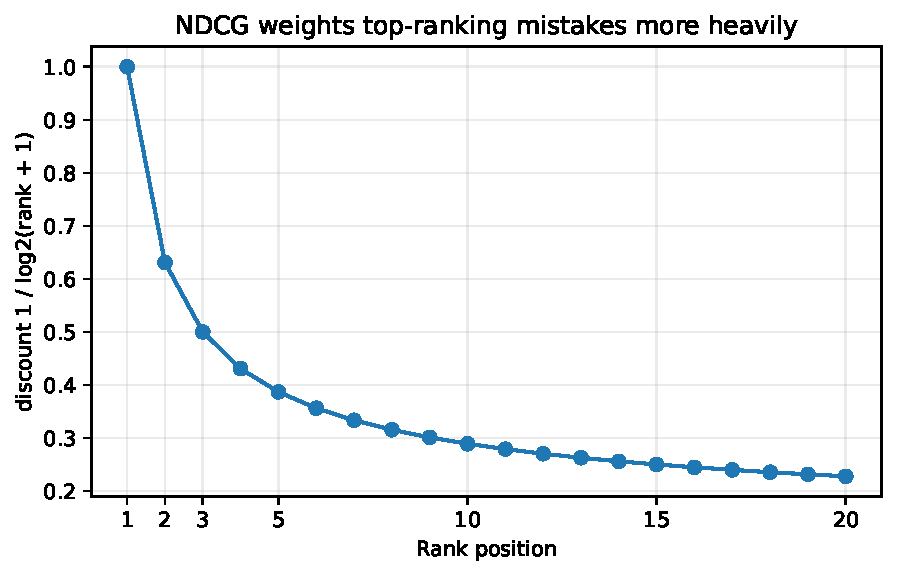
\includegraphics[width=.76\textwidth]{figures/ndcg_discount.pdf}
\caption{The NDCG discount falls fastest at the top, so moving a relevant item between ranks 1 and 2 matters much more than a similar swap deep in the list.}
\label{fig:ranking-ndcg-discount}
\end{figure}
That is why an ordering error near the top can deserve a much stronger training signal than one near rank 100.
LambdaMART uses this idea while retaining boosted-tree stage-wise fitting; see \cref{subsec:trees-lambdamart}.

\subsection{Position bias: clicks mix relevance with exposure}
\label{sec:ranking-position-bias}
A top-ranked item gets more opportunity to be examined than a low-ranked item.
Observed clicks therefore combine at least two effects:
\[
\boxed{
P(\text{click})
\approx
\underbrace{P(\text{examined}\mid\text{position})}_{\text{exposure}}
\times
\underbrace{P(\text{click}\mid\text{examined, relevance})}_{\text{preference}}.
}
\]
Training naively on clicks can make ``was shown high'' look like ``was relevant''.

\begin{figure}[htbp]
\centering
\begin{tikzpicture}[node distance=7mm and 10mm]
\node[flow] (rel) {True relevance};
\node[flow,below=12mm of rel] (pos) {Display position};
\node[yesbox,right=18mm of rel] (click) {Observed click};
\draw[arr] (rel)--(click);
\draw[arr] (pos)--(click);
\end{tikzpicture}
\caption{Click labels are confounded by both user preference and the system's exposure policy.}
\end{figure}

\subsection{Inverse propensity scoring}
\label{sec:ranking-ips}
If the logging policy exposes an item with probability $p_i$, inverse propensity scoring (IPS) weights its observed contribution by roughly
\[
\boxed{
w_i
=
\frac{1}{p_i}.
}
\]
Rarely exposed observations count more because they represent a larger set of opportunities that were usually not shown.
The correction can have high variance:
\[
p_i\rightarrow0
\quad\Rightarrow\quad
w_i\rightarrow\infty.
\]
Practical systems therefore need credible propensity estimates plus clipping/regularisation or explicit exploration where appropriate.

\begin{calloutmemoryhook}
IPS makes rare exposures count more; tiny propensities can make variance explode.
\end{calloutmemoryhook}

\subsection{Evaluation: diagnose the funnel stage}
\label{sec:ranking-evaluation}
Use Recall@K for candidate generation, NDCG/MRR for ordering, and online experiments for product outcomes.
These metrics are defined in \cref{sec:evaluation-retrieval-and-ranking-metrics,sec:evaluation-online-experiments-and-ab-testing}.
Offline ranking gains do not guarantee online user-value gains because historical labels were generated under an earlier exposure policy.

Interleaving can combine results from two rankers into one list for a sensitive direct comparison under the same user/context.
A/B tests remain necessary when the question is broader product impact rather than relative list preference.

\subsection{Degrees of experiment}
\label{sec:ranking-optionality}
\begin{calloutdegreeofexperiment}
Vary candidate sources, user/item representation, embedding dimension, ANN index, candidate count, ranker family, pointwise/pairwise/listwise objective, bias correction, reranker capacity, exploration policy and stage-specific metrics.
\end{calloutdegreeofexperiment}

\begin{calloutmemoryhook}
Retrieve for recall; rank for order; rerank for precision.
\end{calloutmemoryhook}

\section{Use Case: Personalisation}
\label{chap:personalisation}
Ranking asks which item should come first.
Personalisation makes the score depend on who the user is, what the item is, the current context and recent/long-term history:
\[
\boxed{
s
=
f(
\text{user},
\text{item},
\text{context},
\text{history}
).
}
\]

\subsection{From interaction matrix to latent preference space}
\label{sec:personalisation-matrix-factorisation}
Collaborative filtering begins from a sparse user--item interaction matrix.
Matrix factorisation approximates it with low-dimensional user and item vectors:
\[
\underbrace{R}_{N_{\text{users}}\times N_{\text{items}}}
\approx
\underbrace{U}_{N_{\text{users}}\times N_{\text{latent dims}}}
\underbrace{V^\top}_{N_{\text{latent dims}}\times N_{\text{items}}},
\qquad
\underbrace{\hat r_{u,i}}_{\text{predicted preference}}
=
z_u^\top z_i.
\]
The low-rank prerequisite is in \cref{sec:foundations-eigenstructure-and-low-rank-structure}.

\begin{figure}[htbp]
\centering
\begin{tikzpicture}[node distance=8mm and 13mm]
\node[flow] (user) {User ID};
\node[yesbox,right=of user] (uv) {Latent user\\vector};
\node[flow,below=14mm of user] (item) {Item ID};
\node[yesbox,right=of item] (iv) {Latent item\\vector};
\node[flow,right=18mm of uv] (dot) {Dot product};
\node[yesbox,right=of dot] (score) {Preference\\score};
\draw[arr] (user)--(uv);\draw[arr] (item)--(iv);
\draw[arr] (uv)--(dot);\draw[arr] (iv)--(dot);\draw[arr] (dot)--(score);
\end{tikzpicture}
\caption{Matrix factorisation compresses sparse user--item behaviour into a shared latent geometry.}
\end{figure}

\begin{calloutbias}
If user--item preferences have low-dimensional latent structure, matrix factorisation shares statistical strength across sparse interactions; idiosyncratic preferences outside that structure are harder to represent.
\end{calloutbias}

\subsection{Two towers generalise stored latent vectors}
\label{sec:personalisation-two-tower}
A stored user/item vector cannot naturally explain a new identity with no interaction history.
Two-tower models replace lookup-only representations with learned functions:
\[
z_{\text{user}}
=
f_\theta(\text{history, session, context}),
\qquad
z_{\text{item}}
=
g_\phi(\text{text, image, metadata}).
\]
This connects personalisation directly to the retrieval mechanism in \cref{sec:ranking-retrieval}.
Content features let new items acquire a useful representation before many collaborative interactions exist.

\subsection{Cold start: combine collaborative and content evidence}
\label{sec:personalisation-cold-start}
New users/items have little collaborative signal.
Useful fallbacks include content encoders, popularity priors, onboarding choices and rapidly updated session features.
The system therefore often moves from
\[
\text{collaborative only}
\quad\rightarrow\quad
\boxed{\text{collaborative + content + context}}.
\]
The exact mixture can change as interaction history accumulates.

\subsection{Long-term preference versus session intent}
\label{sec:personalisation-timescales}
A user can have stable months-long interests while exhibiting a very different current-session goal.
One representation can therefore combine multiple timescales:
\[
\underbrace{z_{\text{user now}}}_{\text{current preference state}}
=
f(
\underbrace{z_{\text{long-term}}}_{\text{persistent preference}},
\underbrace{z_{\text{session}}}_{\text{current intent}},
\underbrace{\text{context}}_{\text{time/device/location-like context}}
).
\]
Streaming is valuable when the session state changes faster than the model parameters need to be retrained.

\subsection{Temporal decay: encode how quickly preference becomes stale}
\label{sec:personalisation-temporal-decay}
A simple recency rule weights old interactions less:
\[
\boxed{
\underbrace{w(\Delta t)}_{\text{interaction weight}}
=
2^{-\Delta t/\underbrace{T_{1/2}}_{\text{behaviour half-life}}}.
}
\]
\figpdf[.76\textwidth]{temporal_decay}{Different half-lives encode different assumptions about how quickly past behaviour stops predicting current intent.}
A small $T_{1/2}$ forgets quickly; a large one gives long-term history more influence.
The correct decay rate is domain-dependent rather than a universal recommendation.

\begin{calloutbias}
If recent behaviour predicts current intent better than old behaviour, temporal decay is useful; stable long-term preferences can make aggressive decay throw away signal.
\end{calloutbias}

\subsection{The recommendation feedback loop}
\label{sec:personalisation-feedback-loop}
A recommender changes what the user sees, and those exposures create the interaction data used to train its successor.
The data distribution is therefore partly policy-generated:
\[
\boxed{
P(\text{future training data})
=
P(
\text{observations}
\mid
\text{deployed recommender}
).
}
\]

\begin{figure}[htbp]
\centering
\begin{tikzpicture}[node distance=7mm and 9mm]
\node[flow] (rec) {Recommender};
\node[flow,right=of rec] (show) {Chooses\\exposure};
\node[flow,right=of show] (user) {User\\interaction};
\node[flow,right=of user] (logs) {Logged\\data};
\node[flow,right=of logs] (train) {Next training\\dataset};
\draw[arr] (rec)--(show);\draw[arr] (show)--(user);\draw[arr] (user)--(logs);\draw[arr] (logs)--(train);
\draw[arr,rounded corners] (train.south)--++(0,-.75)--([yshift=-.75cm]rec.south)--(rec.south);
\end{tikzpicture}
\caption{Personalisation is a closed-loop system: current recommendations help generate future labels.}
\end{figure}

\subsection{Popularity bias and self-reinforcement}
\label{sec:personalisation-popularity}
Popular items are exposed more, receive more interactions, become easier to estimate, and can then be scored even higher:
\[
\text{popularity}
\rightarrow
\text{exposure}
\rightarrow
\text{interactions}
\rightarrow
\text{training signal}
\rightarrow
\text{future exposure}.
\]
This does not prove popularity is undesirable; it means observed popularity partly reflects the system that generated exposure.
Position-bias correction in \cref{sec:ranking-position-bias,sec:ranking-ips} addresses one part of this general feedback problem.

\subsection{Exploration versus exploitation}
\label{sec:personalisation-exploration}
Always selecting the current highest score exploits existing knowledge but can prevent the system from learning about underexposed alternatives.
Exploration deliberately spends some immediate reward to gain information:
\[
\underbrace{\text{exploit}}_{\text{best current estimate}}
\quad\longleftrightarrow\quad
\underbrace{\text{explore}}_{\text{learn uncertain alternatives}}.
\]
Without exploration, ``never shown'' can become ``never observed'' and then ``never learned to be good''.
Bandit methods formalise this trade-off when actions influence which rewards are observed.

\subsection{Fast state updates versus slow parameter updates}
\label{sec:personalisation-streaming-retraining}
A production recommender often has two update loops:

\begin{figure}[htbp]
\centering
\begin{tikzpicture}[node distance=8mm and 10mm]
\node[flow] (events) {User events};
\node[flow,above right=7mm and 13mm of events] (fast) {Fast stream\\session state};
\node[yesbox,right=of fast] (online) {Online\\ranker};
\node[flow,below right=7mm and 13mm of events] (store) {Historical\\store};
\node[flow,right=of store] (train) {Offline\\retraining};
\node[yesbox,right=of train] (model) {New model\\version};
\draw[arr] (events)--(fast);\draw[arr] (fast)--(online);
\draw[arr] (events)--(store);\draw[arr] (store)--(train);\draw[arr] (train)--(model);
\draw[arr,rounded corners] (model.north)--++(0,.7)--([yshift=.7cm]online.south)--(online.south);
\end{tikzpicture}
\caption{Fast features capture current intent; slower retraining changes the underlying model parameters.}
\end{figure}

A metric drop or drift alert should trigger diagnosis before retraining because data-pipeline failures, inventory changes, delayed labels and real preference shifts need different fixes.
The production-system monitoring stack in \cref{sec:systems-monitoring,sec:systems-drift-retraining} provides the broader framework.

\subsection{Degrees of experiment}
\label{sec:personalisation-optionality}
\begin{calloutdegreeofexperiment}
Vary user representation, item representation, long-term/session weighting, history window, temporal decay, candidate generation, ranking objective, exploration policy, feature freshness, propensity correction and retraining cadence/trigger.
\end{calloutdegreeofexperiment}

\begin{calloutmemoryhook}
The recommender changes the data that trains the next recommender.
\end{calloutmemoryhook}

\section{Use Case: PDE Solvers}
\label{chap:usecase_pde_solvers}

\section{Use Case: Experimental Sensor Regimes}
\label{sec:sensors}
Suppose we have unlabelled measurements from an experimental apparatus collected across operating conditions, with occasional suspected faults but no trusted regime labels.
The goal could be to describe recurring operating states, identify transitions, or prioritise surprising runs; these are \emph{different output requirements} on the same dataset.

\begin{center}
    \begin{tikzpicture}[font=\scriptsize,>=stealth]
     \tikzset{ulstage/.style={draw=black!40,rounded corners=1pt,align=center,minimum height=9mm,inner sep=3pt}}
     \node[ulstage,text width=22mm] (raw) at (-5.5,0) {Sensor readings\\time / apparatus ID};
     \node[ulstage,text width=22mm] (prep) at (-2.75,0) {Scale / clean\\train-only fit};
     \node[ulstage,text width=22mm] (rep) at (0,0) {Representation\\features / PCA};
     \node[ulstage,text width=22mm] (model) at (2.75,0) {Structure\\clusters / scores};
     \node[ulstage,text width=22mm] (valid) at (5.5,0) {Validation\\stability / utility};
     \foreach \a/\b in {raw/prep,prep/rep,rep/model,model/valid}{\draw[->] (\a)--(\b);}
     \draw[->,dashed,black!60] (valid.south)--++(0,-.55)-| (rep.south);
     \node[below] at (0,-.72) {reconsider features and assumptions if validation fails};
    \end{tikzpicture}
    \caption{The clustering algorithm is only one stage: feature construction and validation determine whether its structure is meaningful.}
    \label{fig:pipeline}
\end{center}

\textbf{Experimental sequence.}
First, split by time or apparatus where repeated measurements would otherwise leak nearly identical runs across train and validation; fit preprocessing only to the training partition.
Use K-Means as a cheap baseline for compact operating regimes, compare GMM if soft transitions are physically plausible, and test HDBSCAN if groups are curved or rare regimes should remain unassigned.
Compare against hierarchical clustering when understanding sub-regimes at several resolutions matters more than scalability.
If the real requirement is fault triage, compare Isolation Forest and local-density scores against the clustering baselines instead of assuming small clusters are faults.
Inspect whether groups track known nuisance variables (sensor calibration, acquisition batch or ambient temperature) rather than the underlying behaviour of interest.
Finally, freeze the choices and test cluster stability and any downstream fault/retrieval/forecasting gain on unseen data.

\section{Use Case: LLMs}
\label{chap:usecase_LLMs}
\subsection{Training}
\label{sec:modern-llm-training-lifecycle}
Now we have an architecture.
The lifecycle is approximately:

\begin{figure}[htbp]
\centering
\resizebox{.96\linewidth}{!}{%
\begin{tikzpicture}[node distance=7mm and 8mm]
\node[flow] (data) {Internet / books / code / domain data};
\node[flow,right=of data] (clean) {Clean, filter,\\deduplicate};
\node[flow,right=of clean] (tok) {Tokenise};
\node[flow,right=of tok] (pre) {Pretrain};
\node[yesbox,right=of pre] (base) {Base model};
\node[flow,right=of base] (sft) {Supervised\\fine-tuning};
\node[yesbox,right=of sft] (inst) {Instruction\\model};
\node[flow,right=of inst] (pref) {Preference /\\alignment training};
\node[yesbox,right=of pref] (assist) {Assistant};
\draw[arr] (data)--(clean);\draw[arr] (clean)--(tok);\draw[arr] (tok)--(pre);\draw[arr] (pre)--(base);\draw[arr] (base)--(sft);\draw[arr] (sft)--(inst);\draw[arr] (inst)--(pref);\draw[arr] (pref)--(assist);
\end{tikzpicture}}
\caption{The modern LLM training lifecycle: broad predictive pretraining first, then progressively narrower behavioural adaptation.}
\label{fig:modern-llm-training-lifecycle}
\end{figure}

These stages should not be mentally conflated.
The concise versions already appear in \cref{sec:llms-pretraining,sec:llms-sft,sec:llms-preference-optimisation}; here we connect them to the preceding architecture and scaling story.

\subsubsection{Pretraining}
\label{subsec:modern-pretraining}
Consider:
\begin{quote}
The cat sat on the \_\_\_.
\end{quote}

The model predicts a probability distribution, for example:
\begin{center}
\small
\begin{tabular}{lr}
\toprule
Token & Probability \\
\midrule
mat & $0.42$ \\
floor & $0.18$ \\
chair & $0.10$ \\
moon & $0.0001$ \\
\bottomrule
\end{tabular}
\end{center}

During causal-language-model pretraining, we minimise
\[
\mathcal L
=
-\sum_t
\log p_{\theta_{\text{weights}}}(x_t\mid x_{<t}).
\]

Meaning:

\begin{quote}
Assign high probability to the actual next token.
\end{quote}

The data flow is:
\[
[x_1,x_2,x_3,x_4,x_5]
\rightarrow
\underbrace{[x_1,x_2,x_3,x_4]}_{\text{model inputs}}
\rightarrow
\underbrace{[x_2,x_3,x_4,x_5]}_{\text{targets}}.
\]

One sequence gives many predictions simultaneously during training, while causal masking ensures each position sees only valid history.

\textbf{Why next-token prediction learns so much.}
To predict ``The capital of France is \_\_\_'' you need geographical associations.
To predict \code{for i in range(} you benefit from programming syntax.
To predict a detective novel, you benefit from discourse structure and character relationships.

So a very simple objective forces the network to learn whatever statistical structure helps reduce prediction error.
That is one reason language modelling scales surprisingly far.

\paragraph*{Pretraining is not instruction following}
Imagine the input:
\begin{quote}
What is photosynthesis?
\end{quote}

A pure pretrained model has learned:

\begin{quote}
What text probably follows this string?
\end{quote}

It has not necessarily learned the social convention:

\begin{quote}
Produce a concise, useful answer to the user's question.
\end{quote}

That is a different behavioural objective.
Hence post-training.

\subsubsection{Fine-tuning}
\label{subsec:modern-finetuning}
Fine-tuning begins with pretrained parameters
\[
\theta_{\text{pretrained weights}}
\]
and continues training on a narrower dataset.

For instruction tuning:
\[
\underbrace{\text{``Explain gradient descent simply.''}}_{\text{input}}
\longrightarrow
\underbrace{\text{``Gradient descent is...''}}_{\text{target}}.
\]

The resulting gradient updates the pretrained model toward this desired interaction pattern.

\begin{center}
\small
\begin{tabularx}{.91\linewidth}{@{}L{.22\linewidth}YY@{}}
\toprule
 & \textbf{Pretraining} & \textbf{Fine-tuning} \\
\midrule
Data & huge / general & smaller / specialised \\
Goal & learn broad distribution & adapt behaviour/domain/task \\
Cost & enormous & much smaller \\
Starting point & random-ish parameters & pretrained model \\
Output & base model & adapted model \\
\bottomrule
\end{tabularx}
\end{center}

Fine-tuning works because the expensive representational learning already occurred.

\begin{calloutintuition}
Pretraining is the broad education; fine-tuning is learning the specific behaviour and methods needed in one lab or role.
\end{calloutintuition}

\subsubsection{The problem with full fine-tuning}
\label{subsec:modern-full-ft-cost}
Suppose your base model has 70 billion parameters.
Full fine-tuning potentially updates all 70B.
During Adam-like optimisation you may need storage associated with weights, gradients, first moments and second moments.
This becomes very expensive.

And if you want 100 specialised versions, storing 100 complete parameter copies is cumbersome.
That motivates parameter-efficient fine-tuning.
\paragraph{Fine Tuning}LoRA begins with a pretrained weight matrix $\theta_{\text{weights}}$.
Ordinary fine-tuning learns a full update:
\[
\theta'_{\text{weights}}
=
\theta_{\text{weights}}+\Delta\theta.
\]

If
\[
\theta_{\text{weights}}
\in
\mathbb{R}^{N_{\text{output features}}\times N_{\text{input features}}},
\]
then a full $\Delta\theta$ potentially contains
\[
N_{\text{output features}}N_{\text{input features}}
\]
learnable numbers.

LoRA says:

\begin{quote}
Perhaps the useful adaptation lives in a much lower-dimensional subspace.
\end{quote}

Represent the update as
\[
\boxed{
\Delta\theta
=
\theta_{\text{up}}\theta_{\text{down}}
}
\]
where
\[
\theta_{\text{down}}
\in
\mathbb{R}^{N_{\text{adaptation directions}}\times N_{\text{input features}}},
\]
\[
\theta_{\text{up}}
\in
\mathbb{R}^{N_{\text{output features}}\times N_{\text{adaptation directions}}},
\]
and
\[
N_{\text{adaptation directions}}
\ll
N_{\text{input/output features}}.
\]

The base matrix is frozen.
Only the low-rank factors are trained.
This same mechanism is developed in \cref{sec:adaptation-lora-a-parameter-efficient-adaptation-mechanism}; the linear-algebra prerequisite is \cref{subsec:la-span-and-rank}.

\textbf{Why this saves parameters.}
Suppose
\[
\theta_{\text{weights}}
\in
\mathbb{R}^{4096\times4096}.
\]

A full update contains
\[
4096^2=16.8\text{ million parameters}.
\]

LoRA with
\[
N_{\text{adaptation directions}}=8
\]
needs
\[
4096\times8+8\times4096=65{,}536
\]
trainable numbers for that matrix: roughly $256\times$ fewer.

\textbf{LoRA intuition.}
Imagine a full matrix update can change a representation in every conceivable direction.
LoRA says that adapting from ``general language model'' to a particular downstream behaviour may require only a small number of important directions in parameter space.

\begin{calloutbias}
If useful downstream adaptation is approximately low-rank, freezing the base and learning a small low-rank update captures much of the required change; if the task requires many independent adaptation directions, too small a rank becomes restrictive.
\end{calloutbias}

\begin{calloutdegreeofexperiment}
For LoRA, vary rank, update scaling, target modules, dropout, which layers receive adapters and the adaptation dataset.
\end{calloutdegreeofexperiment}

\begin{calloutpractical}
LoRA is a fine-tuning method, not a new Transformer architecture.
At inference, compatible LoRA updates can often be merged into the base matrix as $\theta'_{\text{weights}}=\theta_{\text{weights}}+\theta_{\text{up}}\theta_{\text{down}}$.
\end{calloutpractical}

\subsubsection{RLHF}
\label{subsec:modern-rlhf}
Now suppose supervised fine-tuning gives two answers: one technically correct but unhelpful, and one correct, concise, clear and instruction-following.
Maximum-likelihood SFT only directly trains on provided target responses.
But humans can often more easily say:

\begin{quote}
B is better than A.
\end{quote}

RLHF uses preference information.
The classic pipeline is:

\begin{figure}[htbp]
\centering
\resizebox{.94\linewidth}{!}{%
\begin{tikzpicture}[node distance=7mm and 8mm]
\node[flow] (sft) {1. Supervised\\fine-tuning};
\node[flow,right=of sft] (gen) {Generate several\\candidate answers};
\node[flow,right=of gen] (rank) {Humans rank\\candidates};
\node[flow,right=of rank] (reward) {2. Train reward /\\preference model};
\node[flow,right=of reward] (rl) {3. Optimise\\language-model policy};
\draw[arr] (sft)--(gen);\draw[arr] (gen)--(rank);\draw[arr] (rank)--(reward);\draw[arr] (reward)--(rl);
\end{tikzpicture}}
\caption{Classical RLHF: demonstrations first, then human rankings, then policy optimisation against the learned preference signal.}
\label{fig:modern-rlhf-pipeline}
\end{figure}

The existing broader preference-optimisation framing is in \cref{sec:llms-preference-optimisation}; the ranking-objective connection is in \cref{sec:objectives-ranking-and-preference-objectives}.

\paragraph*{Reward model intuition}
Suppose humans rank
\[
A>B>C.
\]

Train a model that maps prompt plus response to a scalar preference score:
\[
R_{\theta_{\text{reward}}}(x,y).
\]

For example:
\[
A\rightarrow3.2,
\qquad
B\rightarrow1.1,
\qquad
C\rightarrow-0.7.
\]

These are not objective physical units.
They represent learned human preference.

\paragraph*{Then reinforcement learning}
The language model defines a policy
\[
\pi_{\theta_{\text{weights}}}(y\mid x).
\]

The optimisation pushes it toward outputs with higher learned reward:
\[
\max_{\theta_{\text{weights}}}
\mathbb E[R_{\theta_{\text{reward}}}(x,y)].
\]

But blindly maximising the reward model is dangerous statistically: the policy can exploit imperfections in the learned reward function.
So classical RLHF adds a penalty discouraging the policy from moving too far from a reference model.
Conceptually:
\[
\boxed{
\text{objective}
=
\text{preference reward}
-
\beta\,\text{distance from reference policy}
}.
\]

This gives the optimisation a tether.

\paragraph*{SFT vs RLHF}
SFT says:
\begin{quote}
For this input, imitate this desired answer.
\end{quote}

Preference training says:
\begin{quote}
Between these possible behaviours, humans prefer this one.
\end{quote}

So SFT learns \textbf{demonstrations}.
RLHF learns from \textbf{comparative preferences} and then optimises behaviour against them.
Modern post-training includes additional preference-optimisation approaches, but the classical RLHF pipeline remains the right conceptual foundation.


\subsection{Reasoning}
\subsubsection{Reasoning in Latent Space}


\subsection{Prompting, RAG and fine-tuning solve different missing pieces}
\label{sec:llms-prompt-rag-ft}
Choose the intervention according to what must change.

\begin{figure}[htbp]
\centering
\begin{tikzpicture}[node distance=7mm and 10mm]
\node[decisionnode] (q) {What is\\missing?};
\node[yesbox,above right=9mm and 18mm of q] (prompt) {Temporary instruction\\or small context\\$\rightarrow$ prompt};
\node[yesbox,right=25mm of q] (rag) {Changing/private facts\\$\rightarrow$ RAG};
\node[yesbox,below right=9mm and 18mm of q] (ft) {Persistent behaviour\\$\rightarrow$ SFT / LoRA};
\draw[arr] (q)--(prompt);
\draw[arr] (q)--(rag);
\draw[arr] (q)--(ft);
\end{tikzpicture}
\caption{Prompting changes the current context, RAG changes accessible evidence, and fine-tuning changes persistent model behaviour.}
\end{figure}

A useful optionality axis is
\[
    \underbrace{\text{prompt}}_{\text{cheap/reversible}}
    \rightarrow
    \text{RAG}
    \rightarrow
    \text{LoRA}
    \rightarrow
    \text{partial fine-tuning}
    \rightarrow
    \underbrace{\text{full fine-tuning}}_{\text{more invasive}}.
\]
The LoRA mechanism is already derived in \cref{sec:adaptation-lora-a-parameter-efficient-adaptation-mechanism}; QLoRA adds a quantised frozen base in \cref{subsec:adaptation-qlora}.

\subsection{RAG: external evidence as an inference-time memory}
\label{sec:llms-rag}
Retrieval-augmented generation (RAG) separates external knowledge from the language-model weights.
Documents are indexed offline; a query retrieves useful chunks online; those chunks become additional context for generation.

\begin{figure}[htbp]
\centering
\resizebox{\linewidth}{!}{%
\begin{tikzpicture}[node distance=7mm and 7mm]
\node[flow] (docs) {Documents};
\node[flow,right=of docs] (chunks) {Chunk};
\node[flow,right=of chunks] (emb) {Embed};
\node[yesbox,right=of emb] (index) {Vector index};
\node[flow,below=13mm of docs] (query) {User query};
\node[flow,right=of query] (rewrite) {Optional\\rewrite};
\node[flow,right=of rewrite] (qemb) {Query\\embedding};
\node[flow,right=of qemb] (retrieve) {Broad ANN\\retrieval};
\node[flow,right=of retrieve] (rerank) {Precise\\reranking};
\node[yesbox,right=of rerank] (context) {Top context\\chunks};
\node[flow,right=of context] (llm) {LLM};
\node[yesbox,right=of llm] (ans) {Answer};
\draw[arr] (docs)--(chunks);\draw[arr] (chunks)--(emb);\draw[arr] (emb)--(index);
\draw[arr] (query)--(rewrite);\draw[arr] (rewrite)--(qemb);\draw[arr] (qemb)--(retrieve);
\draw[arr] (index.south)--(retrieve.north);
\draw[arr] (retrieve)--(rerank);\draw[arr] (rerank)--(context);\draw[arr] (context)--(llm);\draw[arr] (llm)--(ans);
\end{tikzpicture}}
\caption{RAG separates broad cheap retrieval from expensive precise reranking before the language model sees a small evidence set.}
\end{figure}


A conversational query can be rewritten into a search-specific query before embedding, which can improve retrieval when the raw wording depends on chat context.
The rewrite is itself a model choice: an aggressive rewrite can also distort user intent.


\subsubsection{Chunking: choose the unit that retrieval can retrieve}
\label{subsec:llms-chunking}
Very small chunks are specific but can lose surrounding context.
Very large chunks preserve context but dilute the embedding signal and consume more LLM context.
Overlap reduces boundary failures at the cost of index duplication.
Chunking is therefore a modelling choice:
\[
\boxed{
\text{specific retrieval unit}
\longleftrightarrow
\text{complete local context}
}.
\]

\subsubsection{Bi-encoder retrieval versus cross-encoder reranking}
\label{subsec:llms-bi-cross}
A bi-encoder maps query and document separately:
\[
\underbrace{z_{\text{query}}}_{\text{computed online}}
=f_\theta(q),
\qquad
\underbrace{z_{\text{doc}}}_{\text{precomputed}}
=g_\phi(d),
\qquad
\underbrace{s(q,d)}_{\text{cheap compatibility}}
=z_{\text{query}}^\top z_{\text{doc}}.
\]
This supports vector indexing because document vectors can be stored once.
A cross-encoder instead processes query and candidate document together, allowing richer token-level interaction but requiring one expensive pass per candidate.

\begin{center}
\small
\begin{tabularx}{.94\linewidth}{@{}L{.23\linewidth}YY@{}}
\toprule
 & \textbf{Bi-encoder} & \textbf{Cross-encoder} \\
\midrule
Query/document interaction & Compressed into two vectors & Joint token-level interaction \\
Document preprocessing & Precompute vectors & Must score per query--document pair \\
Typical role & High-recall retrieval & Precision reranking \\
Scaling & Millions of candidates & Tens/hundreds of candidates \\
\bottomrule
\end{tabularx}
\end{center}

\begin{calloutmemoryhook}
Retrieve broadly; rerank precisely.
\end{calloutmemoryhook}

\subsubsection{Approximate nearest neighbours: HNSW versus IVF}
\label{subsec:llms-ann}
Exact nearest-neighbour search compares the query with every stored vector.
Approximate nearest-neighbour (ANN) methods trade a small amount of retrieval exactness for much lower search work.

\begin{figure}[htbp]
\centering
\begin{tikzpicture}[node distance=8mm and 18mm]
\node[flow] (h) {HNSW\\navigate a graph\\of nearby vectors};
\node[flow,right=of h] (i) {IVF\\choose coarse regions\\then search inside};
\node[yesbox,below=10mm of h] (ht) {Main knob:\\graph search breadth};
\node[yesbox,below=10mm of i] (it) {Main knob:\\clusters probed};
\draw[arr] (h)--(ht);
\draw[arr] (i)--(it);
\end{tikzpicture}
\caption{HNSW prunes search by graph navigation; IVF prunes search by coarse spatial partitioning.}
\end{figure}

HNSW usually spends extra memory on graph edges and searches by repeatedly moving toward closer neighbours.
IVF first assigns vectors to coarse centroids, then searches only selected cells.
The index choice should be compared on recall, latency, memory and update behaviour rather than by algorithm name alone.

\begin{calloutdegreeofexperiment}
For RAG, vary chunking, embedding model/dimension, similarity, ANN index, number retrieved, reranker, number of chunks placed in context, query rewriting and generation model.
\end{calloutdegreeofexperiment}

\subsection{MultiAgent}

\subsection{Agentic systems: an LLM inside a stateful control loop}
\label{sec:llms-agents}
A tool-using agent is not simply a larger model.
The language model proposes the next step, an orchestrator owns state/branching/stopping, and tools perform external operations.

\begin{figure}[htbp]
\centering
\begin{tikzpicture}[node distance=8mm and 10mm]
\node[flow] (user) {User request};
\node[flow,right=of user] (llm) {LLM\\proposes next step};
\node[decisionnode,right=of llm] (toolq) {need\\tool?};
\node[flow,above right=5mm and 13mm of toolq] (tool) {Tool / API};
\node[yesbox,right=of tool] (obs) {Observation};
\node[yesbox,below right=5mm and 13mm of toolq] (answer) {Final answer};
\draw[arr] (user)--(llm);
\draw[arr] (llm)--(toolq);
\draw[arr] (toolq)--node[above,font=\scriptsize]{yes}(tool);
\draw[arr] (tool)--(obs);
\draw[arr,rounded corners] (obs.north)--++(0,.6)--([yshift=.6cm]llm.north)--(llm.north);
\draw[arr] (toolq)--node[below,font=\scriptsize]{no}(answer);
\end{tikzpicture}
\caption{The orchestrator turns model calls into a loop; tool execution and approval policy remain outside the language model.}
\end{figure}

High-impact actions can include mandatory human approval gates.
That is a stronger systems guarantee than relying on the model to remember a prose instruction.
Tool protocols standardise how external capabilities are exposed; inference engines independently optimise how model calls are served.

\begin{calloutmemoryhook}
An agent is an LLM inside a stateful control loop with tools.
\end{calloutmemoryhook}

\subsection{LLM research optionality}
\label{sec:llms-optionality}
\begin{center}
\small
\begin{tabularx}{.96\linewidth}{@{}L{.22\linewidth}YY@{}}
\toprule
\textbf{Layer} & \textbf{Knobs} & \textbf{What changes} \\
\midrule
Base model & size, context, architecture & raw modelling capacity / cost \\
Adaptation & prompt, SFT, LoRA, full FT & persistent versus temporary behaviour \\
Retrieval & chunking, embedding, ANN, reranking & external evidence quality / latency \\
Context assembly & number/order of chunks & evidence coverage versus context cost \\
Decoding & temperature, top-$p$, stopping & output diversity and latency \\
Tools & available actions / permissions & external capability and risk \\
Orchestration & state, loops, approval gates & control flow and reliability \\
\bottomrule
\end{tabularx}
\end{center}




\chapter{Interview Questions}

When would you trust CH vs silhouette vs elbow?

elbow heuristic (“argmin second difference”) often picks endpoints (they got k=10). That’s a known failure mode.

If you weren’t allowed to inspect source, how would you infer “latent + nonlinearity”?- Good: correlation + PCA spectrum + conditional independence tests; compare marginals to Gaussian; maybe fit ICA / factor model residuals.
- Bad: “I’d just read _W and _A.”

How would you test heavy tails robustly?- Good: quantiles/QQ plots; tail index estimates; winsorized moments; compare kurtosis stability vs sample size.
- Bad: “Skew/kurtosis once is enough.”


Why does silhouette often choose k=2 on Iris?- Good: strong separation of one species vs the others; silhouette favors coarse separation.
- Bad: “Because Iris has 2 clusters.”


Where does the one-step MSE come from: quantization or sequence model? How would you separate them?- Good: measure reconstruction error of tokenizer alone (decode(encode(Y))) vs prediction error; ablations with oracle next token.
- Bad: “It’s the bigram’s fault.”

Q: “Why outer join and not inner?”  
- Good: “Outer lets us detect missingness across sources; inner would drop partial records and hide data quality issues.”
- Bad: “So we keep everything.”

Explain the Adam optimizer. What do the betas do?

Tell me something that you have a different perspective on that is against the consencus. 

“What does Fisher-Z test actually test, and when is it valid?”- Good: It tests conditional independence under (approx) Gaussian/linear assumptions; otherwise it’s miscalibrated; discuss alternatives (HSIC, kernel CI).
- Bad: “It checks dependence generally.”

Q5: “Earlier you mentioned DeepSpeed + sharding. Which ZeRO stage would you pick for 10B params on 128 GPUs, and why?”     Interview with Deeter Analytics…  
- Good: Concrete: ZeRO-2/3 tradeoffs; optimizer state partitioning; activation checkpointing; comm overlap; throughput vs memory.
- Bad: Vague repetition of “split matrix across GPUs.”

“Why could PCA help KMeans? Give a concrete failure mode without PCA.”

\end{document}
